\chapter{Heritability Estimation}

% Need to stress that we are only calculating the narrow sense heritability
	\section{Introduction}
	The development of \glng{ldsc} has brought great prospect in estimating the heritability of complex disease for one can now estimate the heritability of a trait without requiring the raw genotype. 
	However, as noted by the author of \gls{ldsc}, when the number of causal variants were small, or when working on targeted genotype array, \gls{ldsc} tends to have a larger standard error or might produce unexpected results \citep{Bulik-Sullivan2015}.
	Ideally, we would like to be able to robustly estimate the heritability for all traits, disregarding the genetic architecture (e.g. number of causal \glspl{SNP}).
	
	Moreover, most of the time researchers are interested in the study of dichotomous traits (e.g. ``affected'', ``normal'').
	The estimation of heritability is not as simple as the estimation of heritability for quantitative traits for one will require adjusting case control sampling bias using the liability threshold model.
	For example, it has been suggested that \gls{gcta}, the most popular heritability estimation tools for \gls{GWAS}, will provide highly biased estimates for case control studies \citep{Golan2014}.
	It is therefore important for us to perform empirical simulations to test whether if the estimates from \gls{ldsc} are biased in the same way as \gls{gcta}.
	
	Herein, we would like to develop an alternative algorithm to \gls{ldsc} for heritability estimation using only the test statistics that can provide robust estimates disregarding the genetic architecture of the trait.
	We would also like to inspect whether if \gls{ldsc}'s heritability estimation is robust to prevalence of a trait and if it is biased in the same way as \gls{gcta}.
	This is achieved by performing empirical simulations where we varies the genetic architecture of the traits.
	
	The work in this chapter were done in collaboration with my colleagues who have kindly provide their support and knowledges to make this piece of work possible.
	Dr Johnny Kwan, Dr Miaxin Li and Professor Sham have helped to laid the foundation of this study. 
	Dr Timothy Mak has derived the mathematical proof for our heritability estimation method. 
	Miss Yiming Li, Dr Johnny Kwan, Dr Miaxin Li, Dr Desmond Campbell, Dr Timothy Mak and Professor Sham have helped with the derivation of the standard error of the heritability estimation. 
	Dr Henry Leung has provided critical suggestions on the implementation of the algorithm.
	
	\section{Methodology}	
		The overall aims of this study is to develop a robust algorithm for the estimation of the narrow sense heritability using only the summary statistic from a \gls{GWAS} and to study the performance of the heritability estimation algorithms for different type of traits.
		
		It was noted that in \gls{GWAS}, the test statistic of a particular \gls{SNP} should increases with its own effect size and the effect size from all the other \glspl{SNP} in \gls{LD} with it.
		Based on this property, we may use the information from the \gls{LD} matrix and the test statistic of the \gls{GWAS} \gls{SNP} the estimate the narrow sense heritability.
		
		
		\subsection{Heritability Estimation}
			Remember that the narrow-sense heritability is defined as 
			$$
				h^2 = \frac{\mathrm{Var}(\boldsymbol{y})}{\mathrm{Var}(\boldsymbol{x})}
			$$
			where $\mathrm{Var}(\boldsymbol{x})$ is the variance of the genotype and $\mathrm{Var}(\boldsymbol{y})$ is the variance of the phenotype.
			In a \gls{GWAS}, regression were performed between the \glspl{SNP} and the phenotypes, giving
			\begin{equation}
				\boldsymbol{y}=\boldsymbol{\beta x}+\boldsymbol{\epsilon}
				\label{eq:standardRegress}
			\end{equation}
			where $\boldsymbol{y}$ and $\boldsymbol{x}$ are the standardized phenotype and genotype respectively. 
			$\boldsymbol{\epsilon}$ is then the error term, accounting for the non-genetic elements contributing to the phenotype (e.g. Environment factors).
			Based on \cref{eq:standardRegress}, and by assuming that $\beta \boldsymbol{x}$ independent of $\epsilon$, one can then have
			\begin{align}
				\mathrm{Var}(\boldsymbol{y}) = \mathrm{Var}(\beta \boldsymbol{x})+ \mathrm{Var}(\epsilon) \nonumber\\
				\mathrm{Var}(\boldsymbol{y}) = \beta^2\mathrm{Var}(\boldsymbol{x}) \nonumber\\
				\beta^2= \frac{\mathrm{Var}(\boldsymbol{y})}{\mathrm{Var}(\boldsymbol{x})}
				\label{eq:betaHeri}
			\end{align}
			$\beta^2$ is then considered as the portion of phenotype variance explained by the variance of genotype, which can also be considered as the narrow-sense heritability of the phenotype.
					
			A challenge in calculating the heritability from \gls{GWAS} data is that usually only the test-statistic or p-value were provided and one will not be able to directly calculate the heritability based on \cref{eq:betaHeri}. 
			In order to estimation the heritability of a trait from the \gls{GWAS} test statistic, we exploit the fact that when both $\boldsymbol{x}$ and $\boldsymbol{y}$ are standardized, $\beta^2$ will be equal to the coefficient of determination ($r^2$). 
			Thus, based on properties of the Pearson product-moment correlation coefficient:
			\begin{equation}
				r = \frac{t}{\sqrt{n-2+t^2}}
				\label{eq:pearsonProduct}
			\end{equation}
			where $t$ follows the student-t distribution under the null and $n$ is the number of samples, one can then obtain the $r^2$ by taking the square of \cref{eq:pearsonProduct}
			\begin{equation}
				r^2 = \frac{t^2}{n-2+t^2}
				\label{eq:oriRSquared}
			\end{equation}
			Although $t^2$ follows the F-distribution under the null, it will converge into $\chi^2$ distribution when $n$ is large.
			
			Furthermore, when the effect size is small and $n$ is large, $n\times r^2$ will be approximately $\chi^2$ distributed with mean $\sim 1$. 
			We can then approximate \cref{eq:oriRSquared} as
			\begin{equation}
				r^2= \frac{\chi^2}{n}
				\label{eq:approxChi}
			\end{equation}
			and define the \emph{observed} effect size of each \gls{SNP} to be
			\begin{equation}
			f=\frac{\chi^2-1}{n}
			\label{eq:observedEffect}
			\end{equation}
			
			When there are \gls{LD} between each individual \glspl{SNP}, the situation will become more complicated as each \glspl{SNP}' observed effect will be influenced by other \glspl{SNP} in \gls{LD} with it:
			\begin{equation}
			f_{observed} = f_{true}+f_{LD}
			\label{eq:conceptF}
			\end{equation}
			
			To account for the \gls{LD} structure, we first assume our phenotype $\boldsymbol{y}$ and genotype $\boldsymbol{x}=(x_1,x_2,\dots,x_m)^t$ are standardized and that
			\begin{align*}
				\boldsymbol{y}\sim f(0,1) \\
				\boldsymbol{x}\sim f(0,\boldsymbol{R})
			\end{align*}
			Where $f(m, \boldsymbol{V})$ denote a general distribution with mean $m$ and variance $\boldsymbol{V}$ and $\boldsymbol{R}$ is the \gls{LD} matrix between \glspl{SNP}.
			
			We can then express \cref{eq:standardRegress} in matrix form:
			\begin{align}
				\boldsymbol{y}=\boldsymbol{\beta}^t\boldsymbol{x}+\epsilon
				\label{eq:matrixRegress}
			\end{align}
			Because the phenotype is standardized with variance of 1, the narrow sense heritability can then be expressed as
			\begin{align}
				Heritability& = \frac{\mathrm{Var}(\boldsymbol{\beta}^t\boldsymbol{x})}{\mathrm{Var}(\boldsymbol{y})} \nonumber\\
				&=\mathrm{Var}(\boldsymbol{\beta}^t\boldsymbol{x})
			\end{align}
			If we then assume now that $\boldsymbol{\beta} = (\beta_1, \beta_2,\dots,\beta_m)^t$ has distribution
			\begin{align*}
				\boldsymbol{\beta}&\sim f(0,\boldmath{H})\\
				\boldsymbol{H}&=diag(\boldsymbol{h})\\
				\boldsymbol{h}&=(h_1^2,h_2^2,\dots,h_m^2)^t
			\end{align*}
			where $\boldsymbol{H}$ is the variance of the ``true'' effect. 
			It is shown that heritability can be expressed as %The later part was gone because that will contains E(\beta) which = 0
			\begin{align}
			\mathrm{Var}(\boldsymbol{\beta}^t\boldsymbol{x}) &= \mathrm{E}_x\mathrm{Var}_{\beta|x}(\boldsymbol{\beta}^t\boldsymbol{x})+\mathrm{Var}_x\mathrm{E}_{(\beta|x)}(\boldsymbol{\beta}^t\boldsymbol{x}) \nonumber\\
			&=\mathrm{E}_x(\boldsymbol{x}^t\boldsymbol{\beta\beta}^t\boldsymbol{x}) \nonumber\\ 
			&= \mathrm{E}_x(\boldsymbol{x}^t\boldsymbol{Hx}) \nonumber\\
			&=\mathrm{Tr}(\mathrm{Var}(\boldsymbol{x}\boldsymbol{H})) \nonumber\\
			&=\sum_ih_i^2
			\label{eq:proveHerit}
			\end{align}
			
			Now if we consider the covariance between \gls{SNP}$_i$ ($\boldsymbol{x_i}$) and $\boldsymbol{y}$, we have
			\begin{align}
			 \mathrm{Cov}(\boldsymbol{x}_i,\boldsymbol{y}) &= \mathrm{Cov}(\boldsymbol{x}_i,\boldsymbol{\beta}^t\boldsymbol{x}+\epsilon) \nonumber\\
			 &=\mathrm{Cov}(\boldsymbol{x}_i,\boldsymbol{\beta}^t\boldsymbol{x}) \nonumber\\
			 &=\sum_j{\mathrm{Cov}(\boldsymbol{x}_i,\boldsymbol{x}_j)\boldsymbol{\beta}_j} \nonumber\\
			 &=\sum_j{\boldsymbol{R}_i\boldsymbol{\beta}_j}
			 \label{eq:covPhenoTrue}
			\end{align}
			
			As both $\boldsymbol{x}$ and $\boldsymbol{y}$ are standardized, the covariance will equal to the correlation and we can define the correlation between \gls{SNP}$_i$ and $Y$ as
			\begin{equation}
				\rho_i = \sum_j{R_{ij}\boldsymbol{\beta}_j}
				\label{eq:corPhenoTrue}
			\end{equation}
			In reality, the \emph{observed} correlation usually contains error. 
			Therefore we define the \emph{observed} correlation between \gls{SNP}$_i$ and the phenotype to besss:
			\begin{equation}
			\hat{\rho_i} = \rho_i+\frac{\epsilon_i}{\sqrt{n}}
			\label{eq:obsPheno}
			\end{equation}
			for some error $\epsilon_i$. 
			The distribution of the correlation coefficient about the true correlation $\rho$ is approximately
			$$
				\hat{\rho_i}\sim f(\rho_i, \frac{(1-\rho^2)^2}{n})
			$$
			By making the assumption that $\rho_i$ is close to 0 for all $i$, we have 
			\begin{align*}
				\mathrm{E}(\epsilon_i|\rho_i)&\sim 0\\
				\mathrm{Var}(\epsilon_i|\rho_i)&\sim 1
			\end{align*}
			We then define our $z$-statistic and $\chi^2$-statistic as
			\begin{align*}
				z_i &= \hat{\rho_i}\sqrt{n} \\
				\chi^2_i &= z_i^2\\
				&=\hat{\rho_i}^2n
			\end{align*}
			From \cref{eq:obsPheno} and \cref{eq:corPhenoTrue}, $\chi^2$ can then be expressed as
			\begin{align*}
			\chi^2_i&=\hat{\rho_i}^2n\\
			&=n(\sum_j{R_{ij}\boldsymbol{\beta}_j}+\frac{\epsilon_i}{\sqrt{n}})^2
			\end{align*}
			We have
			\begin{align*}
			\mathrm{E}(\chi^2) &\approx n\boldsymbol{R_i}^t\boldsymbol{HR_i}+1 \nonumber\\
			&=n\sum_j{R^2_{ij}h_i^2}+1
			\end{align*}
			To derive least square estimates of $h_i^2$, we need to find $\hat{h_i^2}$ which minimizes
			\begin{align*}
				\sum_i(\chi_i^2-\mathrm{E}(\chi_i^2))^2&=\sum_i(\chi_i^2-(n\sum_j{R^2_{ij}\hat{h}_i^2}+1))^2
			\end{align*}
			If we define 
			\begin{equation}
			f_i= \frac{\chi_i^2-1}{n}
			\label{eq:defineF}
			\end{equation}
			we got
			\begin{align}
			\sum_i(\chi_i^2-\mathrm{E}(\chi_i^2))^2&=\sum_i(f_i-\sum_j{R^2_{ij}\hat{h}_i^2})^2 \nonumber\\
			&=\boldsymbol{f^tf}-2\boldsymbol{f}^t\boldsymbol{R_{sq}\hat{h}}+\boldsymbol{\hat{h}}^t\boldsymbol{R_{sq}}^t\boldsymbol{R_{sq}\hat{h}}
			\label{eq:leastSquareH}
			\end{align}
			where $\boldsymbol{R_{sq}} = \boldsymbol{R}\circ\boldsymbol{R}$ and $\circ$ denotes the element-wise product (Hadamard product).
			By differentiating \cref{eq:leastSquareH} w.r.t $\hat{h}$ and set to 0, we get
			\begin{align}
				2\boldsymbol{R_{sq}}^t\boldsymbol{R_{sq}}\boldsymbol{\hat{h^2}}-2\boldsymbol{R_{sq}f}&=0 \nonumber\\
				\boldsymbol{R_{sq}}\boldsymbol{\hat{h^2}} &=\boldsymbol{f}
				\label{eq:shrekEq}
			\end{align}
			And the heritability is then defined as 
			\begin{equation}
			\hat{Heritability} = \boldsymbol{1}^t\boldsymbol{R_{sq}}^{-1}\boldsymbol{f}
			\label{eq:fullShrek}
			\end{equation}
			where the $\boldsymbol{1}^t$ were multiplied to $\boldsymbol{R_{sq}}^{-1}\boldsymbol{f}$ to get the sum of the vector $\hat{\boldsymbol{h}}$.
			
		\subsection{Calculating the \Glng{se}}
			From \cref{eq:fullShrek}, we can derive the variance of heritability $H$ as 
			\begin{align}
				\mathrm{Var}(\hat{Heritability})
				&=\boldsymbol{1}^t\boldsymbol{R_{sq}}^{-1}\mathrm{Var}(\boldsymbol{f})\boldsymbol{R_{sq}}^{-1}\boldsymbol{1}
				\label{eq:varHvarf}
			\end{align}
			Therefore, to obtain the variance of $\hat{Heritability}$, we first need to calculate the variance covariance matrix of $\boldsymbol{f}$.
			
			We first consider the standardized genotype $x_i$ with standard normal mean $z_i$ and non-centrality parameter
			$\mu_i$, we have
			\begin{align*}
				\mathrm{E}[x_i]&=\mathrm{E}[z_i+\mu_i]\\
				&=0\\
				\mathrm{Var}(x_i) &=\mathrm{E}[(z_i+\mu_i)^2]+\mathrm{E}[(z_i+\mu_i)]^2\\
				&=\mathrm{E}[z_i^2+\mu_i^2+2z_i\mu_i]+\mu_i^2\\
				&=1 \\
				\mathrm{Cov}(x_i,x_j)&=\mathrm{E}[(z_i+\mu_i)(z_j+\mu_j)]-\mathrm{E}[z_i+\mu_i]\mathrm{E}[z_j+\mu_j]\\
				&=\mathrm{E}[z_iz_j+z_i\mu_j+\mu_iz_j+\mu_i\mu_j]-\mu_i\mu_j\\
				&=\mathrm{E}[z_iz_j]+\mathrm{E}[z_i\mu_j]+\mathrm{E}[z_j\mu_i]+\mathrm{E}[\mu_i\mu_j]-\mu_i\mu_j\\
				&=\mathrm{E}[z_iz_j]
			\end{align*}
			As the genotypes are standardized, therefore $\mathrm{Cov}(x_i,x_j)=\mathrm{Cor}(x_i,x_j)$, we can obtain
			$$
				\mathrm{Cov}(x_i,x_j)=\mathrm{E}[z_iz_j]=R_{ij}
			$$
			where $R_{ij}$ is the \gls{LD} between \gls{SNP}$_i$ and \gls{SNP}$_j$.
			Given these information, we can then calculate $\mathrm{Cov}(\chi_i^2,\chi_j^2)$ as:
			\begin{align*}
				\mathrm{Cov}(\chi_i^2,\chi_j^2)=&\mathrm{E}[(z_i+\mu_i)^2(z_j+\mu_j)^2]-\mathrm{E}[z_i+\mu_i]\mathrm{E}[z_j+\mu_j]\\
				=&\mathrm{E}[z_i^2z_j^2]+4\mu_i\mu_j\mathrm{E}[z_iz_j]-1
			\end{align*}
			Remember that $\mathrm{E}[z_iz_j] = R_{ij}$, we then have
			$$
				\mathrm{Cov}(\chi_i^2, \chi_j^2)=\mathrm{E}[z_i^2z_j^2]+4\mu_i\mu_jR_{ij}-1
			$$
			By definition, 
			$$
				z_i|z_j\sim N(\mu_i+R_{ij}(z_j-\mu_j),1-R_{ij}^2)
			$$
			We can then calculate $\mathrm{E}[z_i^2z_j^2]$ as
			\begin{align*}
				\mathrm{E}[z_i^2z_j^2]&=\mathrm{Var}[z_iz_j]+\mathrm{E}[z_iz_j]^2\\
				&=\mathrm{E}[\mathrm{Var}(z_iz_j|z_i)]+\mathrm{Var}[\mathrm{E}[z_iz_j|z_i]]+R_{ij}^2\\
				&=\mathrm{E}[z_j^2\mathrm{Var}(z_i|z_j)]+\mathrm{Var}[z_j\mathrm{E}[z_i|z_j]]+R_{ij}^2\\
				&=(1-R_{ij}^2)\mathrm{E}[z_j^2]+\mathrm{Var}(z_j(\mu_i+R_{ij}(z_j-\mu_j)))+R_{ij}^2\\
				&=(1-R_{ij}^2)+\mathrm{Var}(z_j\mu_i+R_{ij}z_j^2-\mu_jz_jR_{ij})+R_{ij}^2\\
				&=1+\mu_i^2\mathrm{Var}(z_j)+R_{ij}^2\mathrm{Var}(z_j^2)-\mu_j^2R_{ij}^2\mathrm{Var}(z_j)\\
				&=1+2R_{ij}^2
			\end{align*}
			As a result, the variance covariance matrix of the $\chi^2$ variances represented as
			\begin{equation}
				\mathrm{Cov}(\chi_i^2,\chi_j^2) = 2R_{ij}^2+4R_{ij}\mu_i\mu_j
				\label{eq:finalChi}
			\end{equation}
			After some tedious algebra, we can get 
			\begin{align}
				\mathrm{Var}(H) &=\boldsymbol{1}^t\boldsymbol{R_{sq}}^{-1}\frac{2\boldsymbol{R_{sq}}+4\boldsymbol{R}\circ \boldsymbol{zz}^t}{n^2}\boldsymbol{R_{sq}}^{-1}\boldsymbol{1}
				\label{eq:covH}
			\end{align}
			where $\boldsymbol{z} = \sqrt{\boldsymbol{\chi^2}}$ from \cref{eq:defineF}, with the direction of effect as its sign and $\circ$ is the element-wise product (Hadamard product).
			 
			The problem with \cref{eq:covH} is that it requires the direction of effect. 
			Without the direction of effect, the estimation of \gls{se} will be inaccurate. 
			If we consider that $n\times \boldsymbol{f}+1$ is approximately $\chi^2$ distributed, we might view \cref{eq:shrekEq} as a decomposition of a vector of $\chi^2$ distributions with degree of freedom of 1. 
			Replacing the vector $\boldsymbol{f}$ with a vector of 1, calculate the ``effective number''($e$) of the association\citep{Li2011}. 
			%The problem of this effective number is that they uses the eigenvalue instead of this multiplication.
			%So either we have to explain why we don't follow it (therefore explaining the slidding windows) or we should just avoid mentioning the effective number
			Substituting $e$ into the variance equation of non-central $\chi^2$ distribution will yield
			\begin{equation}
			\mathrm{Var}(H) = \frac{2(e+2H)}{n^2}
			\label{eq:effectiveChi}
			\end{equation}
			\cref{eq:effectiveChi} should in theory gives us an heuristic estimation of the \gls{se}. 
			Moreover, the direction of effect was not required for \cref{eq:effectiveChi}, reducing the number of input required from the user.
			
		\subsection{Case Control Studies}	 
		%Discuss on the liability threshold model. Then the apply orange paper. Then explain how to get the results. 
			When dealing with case control data, we cannot directly use \cref{eq:fullShrek} to estimate the heritability.
			Instead, we will need to employ the concept of liability threshold model from \cref{sec:liability}. 
			
			Based on the derivation of \citet{Yang2010}, the approximate ratio between the \gls{ncp} obtained from case control studies ($NPC_{CC}$) and quantitative trait studies($NCP_{QT}$) were
		
			\begin{equation}
			\frac{NCP_{CC}}{NCP_{QT}} = \frac{i^2v(1-v)N_{CC}}{(1-K)^2N_{QT}}
			\label{eq:originNCPTransform}
			\end{equation}
			where
			\begin{align*}
			 K &= \text{Population Prevalence} \\
			 v &= \text{Proportion of Cases}\\
			 N &= \text{Total Number of Samples}\\
			 i &= \frac{z}{K}\\
			 z &= \text{height of standard normal curve at truncation pretained to K}
			\end{align*}
			
			Using this approximation, we can directly transform the \gls{ncp} between the case control studies and quantitative trait studies.
			As we were transforming the \gls{ncp} of a single study, the sample size in the case control study ($N_{CC}$) and sample size in the quantitative trait study ($N_{QT}$) will be the same, therefore \cref{eq:originNCPTransform} became
			\begin{equation}
			NCP_{QT} = \frac{NCP_{CC}(1-K)^2}{i^2v(1-v)}
			\label{eq:transform}
			\end{equation}
			
			By combining \cref{eq:transform} and \cref{eq:defineF}, we can then have
			\begin{equation}
			f = \frac{(\chi^2_{CC}-1)}{n}\frac{(1-K)^2}{i^2v(1-v)}
			\label{eq:ccConvert}
			\end{equation}
			where $\chi^2_{CC}$ is the test statistic from the case control association test.
			As \cref{eq:ccConvert} is only \cref{eq:defineF} multiply with the constant $\frac{(1-K)^2}{i^2v(1-v)}$, the heritability estimation of case control studies can be simplified to 
			\begin{equation}
			\hat{Heritability} =\frac{(1-K)^2}{i^2v(1-v)} \boldsymbol{1}^t\boldsymbol{R_{sq}}^{-1}\boldsymbol{f}
			\label{eq:caseControlHerit}
			\end{equation}
			
		\subsection{Extreme Phenotype Sampling}
			%Explain why we perform extreme phenotype selections. Explain how that affect the variance of the estimation. Finally, explain how to perform heritability estimation on extreme phenotype. 
			Although the development of \gls{GWAS} now provide unprecedented power to perform hypothesis free association throughout the whole genome, studies of complex traits still require a large amount of samples and most of the time, there were limited budgets.
			It is therefore important to design the experiment in a way where maximum power can be obtained using the smallest amount of samples.
			A common technique is to perform extreme phenotype sampling in the detection stage of the study.
			The extreme phenotype sampling will inflate the frequency distortion between samples from the two extreme end of phenotype and thus increase the statistical power \citep{Guey2011}.
			It was estimated that for a 0.5\% variant with a fivefold effect in the general population, a discovery studies using extreme phenotype sampling requires four times less samples in the replication to achieve 80\% power when compared to studies using random samples \citep{Guey2011}.
			This allows studies to be conducted using a smaller amount of samples with the same degree of power, therefore reducing the cost of the study.
			
			A problem of extreme phenotype sampling was that the variance of the selected phenotype will not be representative of that in the population.
			The effect size are generally overestimated \citep{Guey2011}. 
			Thus, to adjust for this bias, one can multiple the effect size by the ratio between the variance before $V_P$ and after $V_{P'}$ the selection process \citep{Sham2014}, which is equivalent to the multiplication of $\frac{V_{P'}}{V_P}$ to $f$ in \cref{eq:defineF}.
			
			\begin{equation}
			\hat{Heritability} = \frac{V_{P'}}{V_P}\boldsymbol{1}^t\boldsymbol{R_{sq}}^{-1}\boldsymbol{f}
			\label{eq:extremeShrek}
			\end{equation}
			
		\subsection{Inverse of the \glsentrylong {LD} matrix}
			In order to obtain the heritability estimation, we will require to solve \cref{eq:fullShrek}. 
			If $\boldsymbol{R_{sq}}$ is of full rank and positive definite, it will be straight-forward to solve the matrix equation.
			However, more often than not, the \gls{LD} matrix are rank-deficient and suffer from multicollinearity, making it ill-conditioned, therefore highly sensitive to changes or errors in the input.
			To be exact, we can view \cref{eq:fullShrek} as calculating the sum of $\boldsymbol{\hat{h^2}}$ from  \cref{eq:shrekEq}.
			This will involve solving for
			\begin{equation}
			\boldsymbol{\hat{h^2}} = \boldsymbol{R_{sq}}^{-1}\boldsymbol{f}
			\label{eq:shrekInverse}
			\end{equation}
			where an inverse of $\boldsymbol{R_{sq}}$ is observed. 
			
			In normal circumstances (e.g. when $\boldsymbol{R_{sq}}$ is full rank and positive semi-definite), one can easily solve \cref{eq:shrekInverse} using the QR decomposition or LU decomposition.
			However, when $\boldsymbol{R_{sq}}$ is ill-conditioned, the traditional decomposition method will fail.
			Even if the decomposition can be performed, the result tends to be a meaningless approximation to the true $\boldsymbol{\hat{h^2}}$. 
			
			Therefore, to obtain an unique solution, regularization techniques such as the Tikhonov Regularization (also known as Ridge Regression) and \gls{tSVD} has to be performed\citep{Neumaier1998}. 
			There are a large variety of regularization techniques, yet the discussion of which is beyond the scope of this study. 
			In this study, we will focus on the use of \gls{tSVD} in the regularization of the \gls{LD} matrix.
			This is because the \gls{SVD} routine has been implemented in the EIGEN C++ library \citep{eigenweb}, allowing us to implement the \gls{tSVD} method without much concern with regard to the detail of the algorithm. 
			
			To understand the problem of the ill-conditioned matrix and regularization method, we consider the matrix equation $\boldsymbol{Ax}=\boldsymbol{B}$ where $\boldsymbol{A}$ is ill-conditioned or singular with $n\times n$ dimension.
			The \gls{SVD} of $\boldsymbol{A}$ can be expressed as 
			\begin{align}
				\boldsymbol{A} = \boldsymbol{U\Sigma V}^t
				\label{eq:svd}
			\end{align}
			where $\boldsymbol{U}$ and $\boldsymbol{V}$ are both orthogonal matrix and $\boldsymbol{\Sigma}=\mathrm{diag}(\sigma_1,\sigma_2,\dots,\sigma_n)$ is the diagonal matrix of the \emph{singular values}($\sigma_i$) of matrix $\boldsymbol{A}$.
			Based on \cref{eq:svd}, we can get the inverse of $\boldsymbol{A}$ as 
			\begin{align}
				\boldsymbol{A}^{-1}= \boldsymbol{V\Sigma}^{-1}\boldsymbol{U}^t
				\label{eq:svdInverse}
			\end{align}
			Where $
			\boldsymbol{\Sigma}^{-1} = \mathrm{diag}(\frac{1}{\sigma_1},\frac{1}{\sigma_2},\dots,\frac{1}{\sigma_n})$.
			we can then represent $\boldsymbol{Ax}=\boldsymbol{B}$ as
			\begin{align}
				\boldsymbol{Ax}&=\boldsymbol{B} \nonumber\\
				\boldsymbol{U\Sigma V}^t\boldsymbol{x}&=\boldsymbol{B} \nonumber\\
				\boldsymbol{x}&=\boldsymbol{V\Sigma}^{-1}\boldsymbol{U}^t\boldsymbol{B}
				\label{eq:solveBwithError}
			\end{align}
			A matrix $\boldsymbol{A}$ is considered as ill-condition when its condition number $\kappa(\boldsymbol{A})$ is large or singular when its condition number is infinite. 
			One can represent the condition number as $\kappa(\boldsymbol{A})=\frac{\sigma_1}{\sigma_n}$.
			Therefore it can be observed that when $\sigma_n$ is tiny, $\boldsymbol{A}$ is likely to be ill-conditioned and when $\sigma_n=0$, $\boldsymbol{A}$ will be singular. 
			
			One can also observe from \cref{eq:solveBwithError} that when the singular value $\sigma_i$ is small, the error $\epsilon_i$ in \cref{eq:errorB} will be drastically magnified by a factor of $\frac{1}{\sigma_i}$. 
			Making the system of equation highly sensitive to errors in the input.
			
			To obtain a meaningful solution from this ill-conditioned/singular matrix $\boldsymbol{A}$, we may perform the \gls{tSVD} method to obtain a pseudo inverse of $\boldsymbol{A}$.
			Similar to \cref{eq:svd}, the \gls{tSVD} of $\boldsymbol{A}$ can be represented as 
			\begin{alignat}{2}
				&\boldsymbol{A}^+ = \boldsymbol{U\Sigma}_k\boldsymbol{V}^t  &\qquad\text{and}\qquad  &\boldsymbol{\Sigma}_k=\mathrm{diag}(\sigma_1,\dots,\sigma_k,0,\dots,0)
				\label{eq:tsvd}				
			\end{alignat}
			where $\boldsymbol{\Sigma}_k$ equals to replacing the smallest $n-k$ singular value replaced by 0 \citep{Hansen1987}. 
			Alternatively, we can define
			\begin{equation}
			\sigma_i=\begin{cases}
			\sigma_i\qquad\text{for}\qquad\sigma_i\ge t\\
			0\qquad\text{for}\qquad\sigma_i<t
			\end{cases}
			\end{equation}
			where $t$ is the tolerance threshold. 
			Any singular value $\sigma_i$ less than the threshold will be replaced by 0 during the inversion.
			
			By selecting an appropriate $t$, \gls{tSVD} can effectively regularize the ill-conditioned matrix and help to find a reasonable approximation to $x$. 
			A problem with \gls{tSVD} however is that it only work when matrix $\boldsymbol{A}$ has a well determined numeric rank\citep{Hansen1987}.
			That is, \gls{tSVD} work best when there is a large gap between $\sigma_k$ and $\sigma_{k+1}$.
			If a matrix has ill-conditioned rank, then $\sigma_k-\sigma_{k+1}$ will be small.
			For any threshold $t$, a small error can change whether if $\sigma_{k+1}$ and subsequent singular values should be truncated, leading to unstable results. 
			
			According to \citet{Hansen1987}, matrix where its rank has meaning will have well defined rank. 
			The \gls{LD} matrix is the correlation matrix between each individual \glspl{SNP}, the rank of the \gls{LD} matrix is the maximum number of linear independent \glspl{SNP} in the region.
			Because the rank has a meaning, it might likely to have well-defined rank.
			% This was supported by our simulation
			 
			The easiest way to test whether if the threshold $t$ and whether if the matrix $\boldsymbol{A}$ has well-defined rank is to calculate the ``gap'' in the singular value:
			\begin{equation}
			gap = \sigma_k/\sigma_{k+1}
			\label{eq:gapSingular}
			\end{equation}
			a large gap usually indicate a well-defined gap. 
			%\begin{wrapfigure}{L}{3in}
			\begin{figure}
				\caption[Cumulative Distribution of ``gap'' of the LD matrix]{Cumulative Distribution of ``gap'' of the LD matrix, the vertical line indicate the full rank. It can be observed that there is a huge increase in ``gap'' before full rank is achieved. Suggesting that the rank of the LD matrix is well defined}
				\centering
				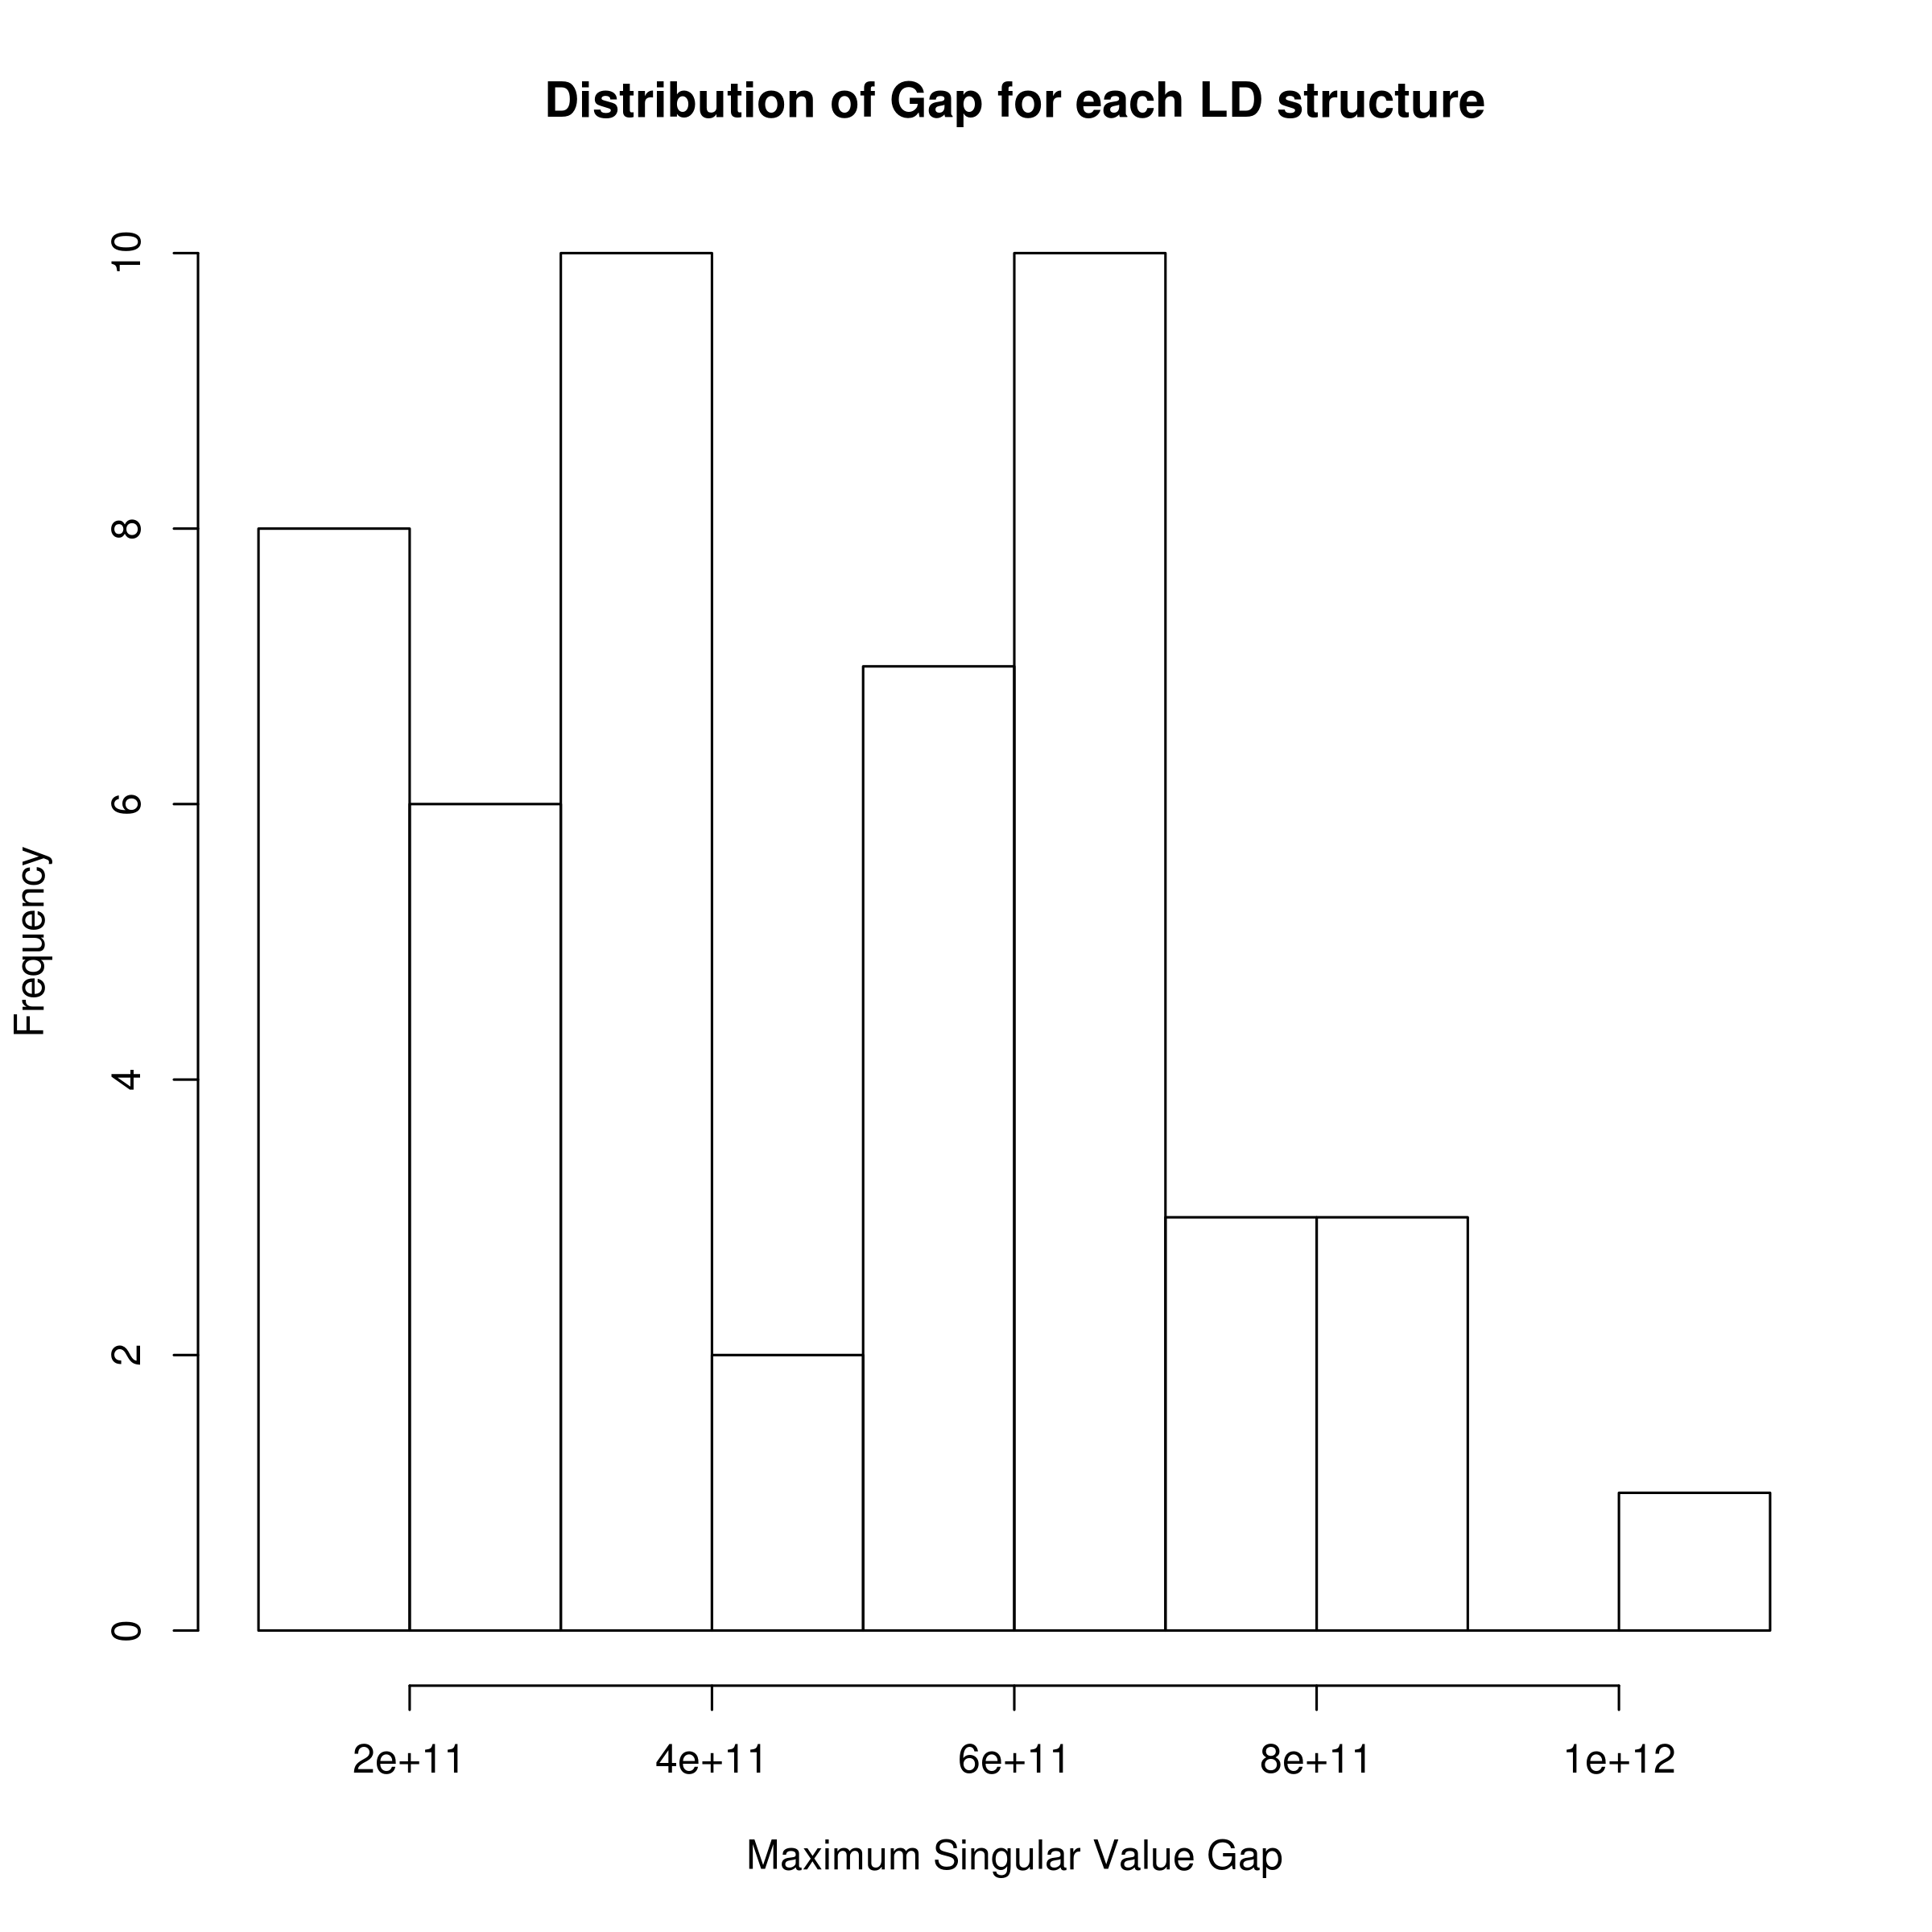
\includegraphics[width=0.5\textwidth]{figure/singular_value_distribution.png}
				\label{fig:singularValueDist}
				\vspace{-20pt}
			\end{figure}
			%\end{wrapfigure}
			In this study, we adopt the threshold as defined in MATLAB, NumPy and GNU Octave: $t=\epsilon\times\mathrm{max}(m,n)\times\mathrm{max}(\boldsymbol{\Sigma})$ where $\epsilon$ is the machine epsilon (the smallest number a machine can define as non-zero). 
			And we perfomed a simulation study to investigate the performance of \gls{tSVD} under the selected threshold.
			Ideally, if the ``gap'' is large under the selected threshold, then \gls{tSVD} will provide a good regularization to the equation. 
			
			1,000 samples were randomly simulated from the HapMap\citep{Altshuler2010} \acrshort{CEU} population with
			1,000 \glspl{SNP} randomly select from chromosome 22. 
			The \gls{LD} matrix and its corresponding singular value were calculated. 
			The whole process were repeated 50 times and the cumulative distribution of the ``gap'' of singular values were plotted (\cref{fig:singularValueDist}). 
			It is clearly show that the \gls{LD} matrix has a well-defined rank with a mean of maximum ``gap'' of 466,198,939,298.
			Therefore the choice of \gls{tSVD} for the regularization is appropriate.
			
			By employing the \gls{tSVD} as a method for regularization, we were able to solve the ill-posed \cref{eq:shrekEq}, and obtain the estimated heritability.
		\subsection{Implementation}
			Our algorithm was implemented using C++ programming languages (version C++11) and the matrix algebra was performed using the EIGEN C++ header library \citep{eigenweb}.
			Although the Armadillo library \citep{Sanderson2010} is much faster in the calculation of \gls{SVD} when compared to EIGEN \citep{Ho2011}, it is dependent on additional libraries such as OpenBLAS. 
			The use of EIGEN therefore simplify the programme installation, making it more user friendly. 
			
			Although \gls{tSVD} allow one to approximate the ill-posed \cref{eq:shrekEq}, it is an $\mathrm{O}(n^3)$ algorithm, making the computation run time prohibitive when the number of \glspl{SNP} is large.
			Unfortunately, the number of \glspl{SNP} in a \gls{GWAS} is generally large, making it impossible for one to calculate the \gls{tSVD} of the whole genome at once. 
			
			If we consider \cref{eq:svd}, the matrix $\boldsymbol{U}$ and $\boldsymbol{V}$ are the eigenvectors of $\boldsymbol{AA}^t$ and $\boldsymbol{A}^t\boldsymbol{A}$ respectively. 
			So for any symmetric matrix such as that of the \gls{LD} matrix, $\boldsymbol{U}$ and $\boldsymbol{V}$ should be the same except for their direction. 
			Thus \cref{eq:svd} reduce into the problem of eigenvalue decomposition where the singular values are the magnitude of the eigenvalues. 
			Although the eigenvalue decomposition is still an $\mathrm{O}(n^3)$ algorithm, it has a smaller constant, therefore has a faster run time when compared to the computation of \gls{SVD}. 
			
			However, even with the use of eigenvalue decomposition in place of \gls{SVD}, the large matrix size is still making the computation of \cref{eq:shrekEq} impossible. 
			Given that it is unlikely inter chromosomal \gls{LD} or for \glspl{SNP} to be in \gls{LD} if they are more than 1 \gls{mb} apart, one can safely assume \glspl{SNP} more than 1\gls{mb} apart are independent of each other. 
			We therefore separate \glspl{SNP} into 1\gls{mb} bins where start of each bin are at least 1\gls{mb} away from each other. 
			Three bins are then combined to form one window, and we perform the decomposition on each windows using \cref{eq:shrekEq} and only update the $\boldsymbol{\hat{h^2}}$ for the bin forming the center of the window.
			We then transverse the genome with step size of 1 bin until $\boldsymbol{\hat{h^2}}$ for all bins were computed. 
			By breaking down the genome into windows, we were able to reduce the matrix dimension which makes the analysis believable.
			Users can also choose distance other than 1\gls{mb} as the distance between bins, allowing for a more flexible usage of the algorithm.
			
		\subsection{Comparing with \glsentrylong{ldsc}}
			% main difference 
			Conceptually, the fundamental hypothesis of \gls{ldsc} and our algorithm were quite different.
			\gls{ldsc} were based on the ``global'' inflation of test statistic and its relationship to the \gls{LD} pattern.
			\gls{ldsc} hypothesize that the larger the \gls{LD} score, the more likely will the \gls{SNP} be able to ``tag'' the causal \gls{SNP} and the heritability can then be estimated through the regression between the \gls{LD} score and the test statistic.
			
			On the other hand, our algorithm focuses more on the per-\gls{SNP} level.
			Our main idea was that the individual test statistic of each \glspl{SNP} is a combination of its own effect and effect from \glspl{SNP} in \gls{LD} with it. 
			Thus, based on this concept, our algorithm aimed to ``remove'' the inflation of test statistic introduced through the \gls{LD} between \glspl{SNP} and the heritability can be calculated by adding the test statistic of all \glspl{SNP} after ``removing'' the inflation. 
			
			Mathematically, the calculation of \gls{ldsc} and our algorithm were also very different. 
			\gls{ldsc} take the sum of all $R^2$ within a 1cM region as the LD score and regress it against the test statistic to obtain the slope and intercept which represent the heritability and amount of confounding factors respectively. 
			In their model, \gls{ldsc} assume that each \glspl{SNP} will explain the same portion of heritability
			\begin{align}
			 \mathrm{Var}(\beta)&=\frac{h^2}{M}\boldsymbol{I}\\
			 M &= \text{number of SNPs}\notag\\
			 \beta &= \text{vector containing per normalized genotype effect sizes}\notag\\
			 I &= \text{identity matrix}\notag\\
			 h^2 &= \text{heritability}\notag
			\end{align}
			
			As for our algorithm, the whole \gls{LD} matrix were used and inverted to decompose the \gls{LD} from the test statistic. 
			There were no assumption of the amount of heritability explained by each \glspl{SNP}. 
			However, our algorithm does assumed that the null should be 1 and therefore cannot detect the amount of confounding factors.  
			
	\section{Comparing Different LD correction Algorithms}
		\label{sec:ldSim}
		% Might want to remove this section as we no longer use this correction
		Another important consideration in our algorithm is the bias in \gls{LD}.
		In reality, one does not have the population \gls{LD} matrix, instead we have to estimate he \gls{LD} based on various reference panels such as those from the 1000 genome project\citep{Project2012} or the HapMap project\citep{Altshuler2010}.
		These reference panels were a subsamples from the whole population and therefore \gls{LD} estimated from the reference panels usually contains sampling bias.
		Under normal circumstances, because the symmetric nature of sampling error, one would expect there to be little to no bias in the estimated \gls{LD}.
		However, in our algorithm , the $R^2$ is required for the estimation of heritability (\cref{eq:fullShrek}).
		Because we were using the squared \gls{LD}, the sampling error will also be squared, generating a positive bias. 
		
		On average, there were around 500 samples for each super population from the 1000 genome project reference panel.
		Given the relatively small sample size, the sampling bias might be high, therefore lead to systematic bias in the heritability estimation in our algorithm.
		
		To correct for the bias, we would like to apply a \gls{LD} correction algorithm to correct for the bias in the sample \gls{LD}.
		Different authors \citep{Weir1980,Wang2007} have proposed methods for the correction of sample $R^2$ and can be applied for the correction of sample bias in \gls{LD}.
		Therefore we considered the following $R^2$ correction algorithms:
		\begin{align}
		\text{Ezekiel}: \tilde{R^2}&= 1-\frac{n-1}{n-2}(1-\hat{R^2})\label{eq:ezekiel} \\
		\text{Olkin-Pratt}: \tilde{R^2}&=1-\frac{(n-3)(1-\hat{R^2})}{n-2}(1+\frac{2(1-\hat{R^2})}{n})\label{eq:okin} \\
		\text{Pratt}: \tilde{R^2}&=1-\frac{(n-3)(1-\hat{R^2})}{n-2}(1+\frac{2(1-\hat{R^2})}{n-3.3})\label{eq:pratt} \\
		\text{Smith}: \tilde{R^2}&=1-\frac{n}{n-1}(1-\hat{R^2}) \label{eq:smith}\\
		\text{Weir}: \tilde{R^2}&=\hat{R^2}-\frac{1}{2n} \label{eq:weir}
		\end{align}
		where $n$ is the number of samples used to calculate the $R^2$, $\hat{R^2}$ is the sample $R^2$ and $\tilde{R^2}$ is the corrected $R^2$.
		
		In order to assess the performance of each individual correction methods, we perform simulations to compare the performance of our algorithm using different \gls{LD} bias correction algorithms.
		Most importantly, we would like to assess the performance of different algorithms not only under one specific \gls{LD} range, but also under the complex \gls{LD} structure observed in real life scenarios.
		First, 5,000 \glspl{SNP} with \gls{maf} $\ge0.1$ were randomly selected from chromosome 22 from the 1000 genome \gls{CEU} haplotypes and were used as an input to HAPGEN2 \citep{Su2011} to simulate 1,000 individuals.
		HAPGEN2 is a simulation tools which simulates new haplotypes as an imperfect mosaic of haplotpyes from a reference panel and the haplotypes that have already been simulated using the \textit{Li and Stephens} (LS) model of \gls{LD} \citep{Li2003}.
		This allow us to simulate genotypes with \gls{LD} structures comparable to those observed in \gls{CEU} population. 
		Of those 5,000 \glspl{SNP}, 100 of them were randomly selected as the causal variant. 
		\citet{Orr1998} suggested that the exponential distribution can be used to approximate the genetic architecture of adaptation. 
		As a result of that, we used the exponential distribution with $\lambda=1$ as an approximation to the effect size distribution:
		\begin{align}
		\theta&=\mathrm{exp}(\lambda=1)\notag\\
		\beta&=\pm\sqrt{\frac{\theta \times h^2}{\sum \theta}}
		\label{eq:randomEffect}
		\end{align}
		with a random direction of effect.
		The simulated effects were then randomly distributed to each causal \glspl{SNP}.
			
		Using the normalized genotype matrix of the causal \glspl{SNP} of all individual ($\boldsymbol{X}$), the vector of effect size ($\boldsymbol{\beta}$) we can simulate a phenotype with target heritability of $h^2$ as
		\begin{align}
		\epsilon_i&\sim N(0,\mathrm{Var}(\boldsymbol{X\beta})\frac{1-h^2}{h^2} )\notag\\
		\boldsymbol{\epsilon} &= (\epsilon_1,\epsilon_2,...,\epsilon_n)^t\notag\\
		\boldsymbol{y} &= \boldsymbol{X\beta}+\boldsymbol{\epsilon}
		\label{eq:simulationOfPhenotype}
		\end{align}
		To simulate the whole spectrum of heritability, we varies the target $h^2$ from 0 to 0.9 with increment of 0.1.
		
		The test statistics of association between the genotype and phenotype were then calculated using PLINK \citep{Purcell2007}.
		Resulting test statistic were then input to our algorithm to estimate the heritability, using different \gls{LD} correction algorithms.
		An independent 500 samples, a size roughly correpsond to the average sample size of each super population form the 1,000 genome project,  were simulated as a reference panel for the calculation of \gls{LD} matrix.
		This is because in reality, one usually doesn't have assess to the sample genotype and has to rely on an independent reference panel for the calculation of \gls{LD} matrix. 
		Thus this simulation procedure should provide a realistic representation of how the algorithm was commonly used in real life scenario.
		
		The whole process will be repeated 50 times such that a distribution of the estimate can be obtained. 
		In summary, we simulate a large population of samples (e.g. $50\times1,000+500 = 50,500$) where 500 samples were randomly selected as a reference panel. 
		In the subsequent iteration of simulation, 1,000 samples were randomly selected from the population \textit{without replacement} and estimation were performed.
		\begin{enumerate}
			\item Randomly select 5,000 \glspl{SNP} with \gls{maf}$>0.1$ from chromosome 22
			\item Simulate 500 samples using HAPGEN2 and used as a reference panel
			\item Randomly generate 100 effect size with following \cref{eq:randomEffect}
			\item Randomly assign the effect size to 100 \glspl{SNP} with heritability from 0 to 0.9 (increment of 0.1)
			\item Simulate 1,000 samples using HAPGEN2 and calculate their phenotype according to \cref{eq:simulationOfPhenotype} 
			\item Perform heritability estimation using our algorithm with different ways of \gls{LD} correction
			\item Repeat step 5-6 50 times
		\end{enumerate}
		
		\section{Comparison with Other Algorithms}
		After identifying the optimal \gls{LD} correction algorithm, we would like to compare our algorithm to existing methods for the performance in estimating the narrow sense heritability.
		It is important for us to consider most if not all conditions in our simulation. 
		Therefore, we would like to simulate quantitative traits and case control studies with different number of causal \glspl{SNP}; quantitative traits with extreme effect sizes; and last but not least, quantitative traits with extreme phenotype sampling.
		
		Currently, the only other algorithm that is capable to estimate the narrow sense heritability using only test statistic is the \gls{ldsc} \citep{Bulik-Sullivan2015}. 
		On the other hand, \gls{gcta} \citep{Yang2011} is commonly used for heritability estimation in \gls{GWAS} data. 
		Therefore, we choose to compare the performance of our algorithm to that of \gls{ldsc} and \gls{gcta}.
		It is important to note that as we are assessing the performance of the algorithms through controlled simulation, there should be little confounding factors. 
		For \gls{ldsc}, the default intercept estimation function allows it to estimate and correct for confounding factors with an increase in \gls{se}. 
		The simulation will therefore be unfair to \gls{ldsc} with intercept estimation, as the \gls{se} is increased yet there are little confounding factors for it to correct.
		Thus, we also simulate \gls{ldsc} with a fixed intercept (-{}-no-intercept) parameters to avoid bias against \gls{ldsc}.	
		
		\subsection{Sample Size}
			One important consideration in our simulation was the number of sample simulated. 
			The sample size was the most important parameter in determining the standard error of the heritability estimation. 
			As sample size increases, study will be more representative of the true population. 
			The increased number of information also means a better estimation of parameters, therefore a smaller \acrfull{se}.
			% awk -F "\t" '{print $2"\t"$9}' full | uniq | sed -e 's/[^0-9[:space:]]//g' | awk '{for(i=2;i<=NF;++i)j+=$i; print $1" "j; j=0}' | sort | uniq  %script for text mining
			Based on information from \gls{GWAS} catalog\citep{Welter2014}, we calculate the sample size distribution using simple text mining and exclude studies with conflicting sample size information in multiple entries. 
			The average sample size for all \gls{GWAS} recorded on the \gls{GWAS} catalog was 7,874, with a median count of 2,506 and a lower quartile at 940 (\cref{fig:gwasCata}). 
			We argue that if the algorithm works for studies with a small sample size (e.g lower quartile sample size), then it should perform even better when the sample size is larger. 
			Thus, we only simulate 1,000 samples in our simulation, which roughly represent the lower quartile sample size range.
				
			\begin{wrapfigure}{R}{8cm}
				\centering
				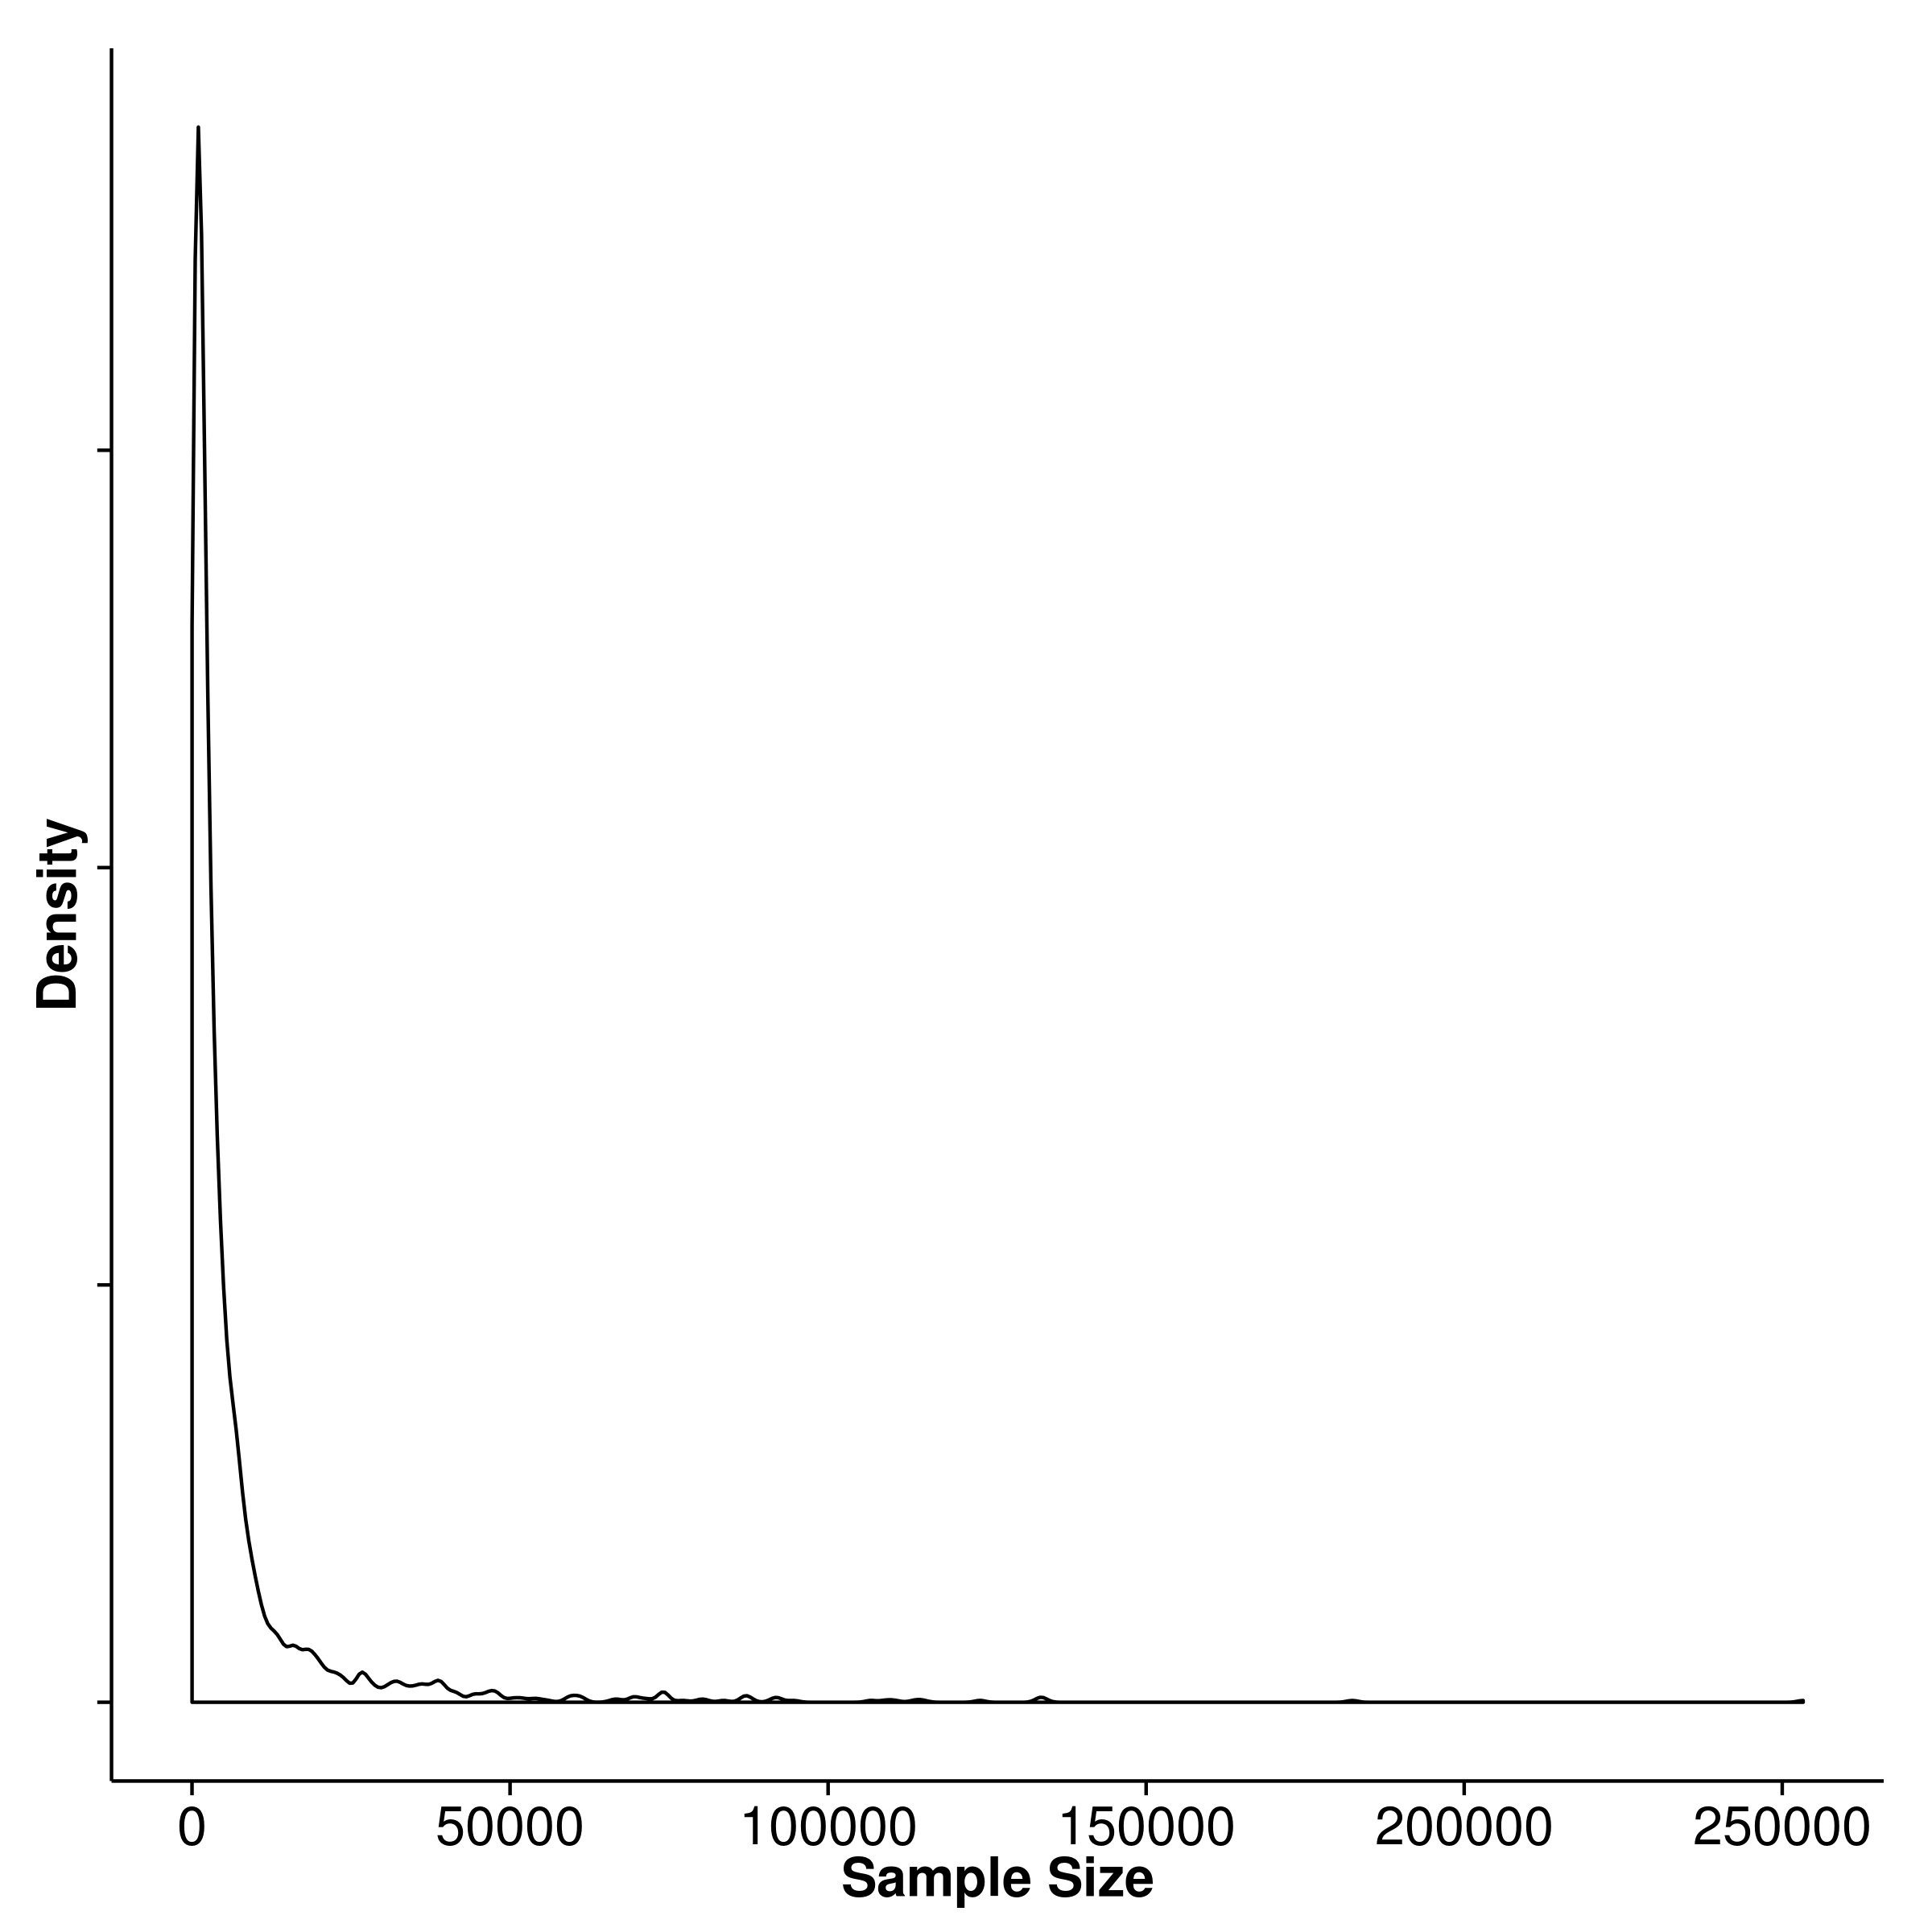
\includegraphics[width=0.5\textwidth]{figure/gwasSampleSize.png}
				\caption[GWAS Sample Size distribution]{
					\gls{GWAS} sample size distribution.
				}
				\label{fig:gwasCata}
			\end{wrapfigure}
		\subsection{Number of SNPs in Simulation}
			Another consideration in the simulation was the number of \glspl{SNP} included.
			In a typical \gls{GWAS} study, there are usually a larger number of \glspl{SNP} when compared to the sample size. 
			For example, in the \gls{pgc} \glng{scz} \gls{GWAS}, more than 9 million \glspl{SNP} were included, with around 700,000 \glspl{SNP} on chromosome 1.
			In reality, the estimation of heritability based on 700,000 \glspl{SNP} can be done quickly.
			However, in our simulation, we will repeat the calculation $50(\text{iteration})\times10(\text{number of heritability})=500$ times for \emph{each} condition tested. 
			The time required to finish all the simulation quickly becomes infeasible given the large amount of \glspl{SNP}.
			To compromise, we simulate a total of 50,000 \glspl{SNP} from chromosome 1 as a balance between run time of simulation and the total \glspl{SNP} simulated.
			With 50,000 \glspl{SNP}, there are roughly 200 \glspl{SNP} within a 1 \gls{mb} region.
		\subsection{Genetic Architecture}
			Of all simulation parameter, the genetic architecture was the most complicated and important parameter. 
			The \gls{LD} pattern, the number of causal \glspl{SNP}, the effect size of the causal \glspl{SNP} and the heritability of the trait were all important factors contribute to the genetic architecture of a trait. 
		
			First and foremost, because the aim of the algorithm was to estimating the heritability of the trait, it is important that the algorithm works for traits from different heritability spectrum.
			We therefore simulate traits with heritability ranging from 0 to 0.9, with increment of 0.1.
		
			Secondly, in real life scenario, the ``causal'' variant might not be readily included on the \gls{GWAS} chip and were only ``tagged'' by \glspl{SNP} included on the \gls{GWAS} chip.
			However, to simplify our simulation, all ``causal'' variants were included in our simulation (e.g. perfectly ``tagged'')
		
			Thirdly, to obtain a realistic \gls{LD} pattern, we simulate the genotypes using the HAPGEN2 programme\citep{Su2011}, using the 1000 genome \gls{CEU} haplotypes as an input.
			In a typical \gls{GWAS} , one usually only have power in detecting ``common variants'', defined as variants with \gls{maf} $\ge 0.05$.
			We therefore only consider scenario with ``common'' variants and only use \glspl{SNP} with \gls{maf} $\ge0.05$ in the \gls{CEU} haplotypes as an input to HAPGEN2 to simulate 1,000 samples.
			
			Finally, we would like to simulate traits with different inheritance model such as oligogenic traits and polygenic traits.
			We therefore varies the number of causal \glspl{SNP} ($k$) with $k\in\{5, 10, 50, 100, 500\}$.
			The effect size were then simulated using \cref{eq:randomEffect} and the phenotype were simulated using \cref{eq:simulationOfPhenotype}.
			
			For \gls{gcta}, the sample genotypes were provided to calculate the genetic relationship matrix and the sample phenotype were used in combination with the genetic relationship matrix to estimate the heritability.
			
			On the other hand, for \gls{ldsc} and our algorithm, an independent 500 samples were simulated as the reference panel for the calculation of \gls{LD} scores and \gls{LD}matrix, mimicking real life scenario where an independent reference panel were used. 
			The genotype association test statistics calculated from PLINK and the \gls{LD} score / \gls{LD} matrix were then used for the estimation of heritability for \gls{ldsc} and our algorithm respectively. 
			
			The whole process will be repeated 50 times such that a distribution of the estimate can be obtained.
			10 independent population were simulated and the whole processed were repeated.
			In summary, the simulation follows the following procedures:
			\begin{enumerate}
				\item Randomly select 50,000 \glspl{SNP} with \gls{maf}$>0.05$ from chromosome 1
				\item Simulate 500 samples using HAPGEN2 and used as a reference panel
				\item Randomly generate $k$ effect size with $k \in \{5,10,50,100,500\}$ following \cref{eq:randomEffect}, with heritability ranging from 0 to 0.9 (increment of 0.1)
				\item Randomly assign the effect size to $k$ \glspl{SNP}
				\item Simulate 1,000 samples using HAPGEN2 and calculate their phenotype according to \cref{eq:simulationOfPhenotype}
				\item Perform heritability estimation using our algorithm, \gls{gcta}, \gls{ldsc} with fixed intercept and \gls{ldsc} with intercept estimation.
				\item Repeat step 5-6 50 times
				\item Repeat step 1-7 10 times
			\end{enumerate}
		
		\subsection{Extreme Effect Size}
		On top of the original quantitative trait simulation, another condition we were interested in was the performance of the algorithms when there is a small amount of \glspl{SNP} with a much larger effect size.
		This can be observed in disease such as Hirschsprung's disease.
		The Hirschsprung's disease is a congenital disorder where deleterious mutations on \textit{RET} account for $\approx$50\% of the familial cases yet there is still missing heritability, suggesting that there might be more variants with small effects that have not been identified \citep{Gui2013}.
		
		To simulate extreme effect size, we consider scenarios where $m$ \glspl{SNP} accounts 50\% of all the effect size with $m\in\{1,5,10\}$.
		The effect size was then calculated as
		\begin{align}
		\beta_{eL} &= \pm\sqrt{\frac{0.5h^2}{m}} \notag\\
		\beta_{eS} &= \pm\sqrt{\frac{0.5h^2}{100-m}} \notag\\
		\beta &= \{\beta_{eL}, \beta_{eS}\}
		\label{eq:extremEffect}
		\end{align}
		The effect size were then randomly assigned to 100 causal \glspl{SNP} and phenotype will be calculated as in \cref{eq:simulationOfPhenotype}.
		The simulation procedure then becomes
		\begin{enumerate}
			\item Randomly select 50,000 \glspl{SNP} with \gls{maf}$>0.1$ from chromosome 1
			\item Simulate 500 samples using HAPGEN2 and used as a reference panel
			\item Randomly generate 100 effect size where $m$ has extreme effect, following \cref{eq:extremEffect}, with $m\in\{1,5,10\}$
			\item Randomly assign the effect size to 100 \glspl{SNP}
			\item Simulate 1,000 samples using HAPGEN2 and calculate their phenotype according to \cref{eq:simulationOfPhenotype}
			\item Perform heritability estimation using our algorithm, \gls{ldsc} with fixed intercept, \gls{ldsc} with intercept estimation and \gls{gcta}
			\item Repeat step 5-6 50 times
			\item Repeat step 1-7 10 times
		\end{enumerate}
		
		\subsection{Case Control Studies}
		The simulation of case control studies was similar to the simulation of quantitative trait. 
		However, there were two additional parameters to consider: the population prevalence and the observed prevalence.
		These parameters were required to simulate the samples under a liability model for case control studies.

		Although there were only two additional parameter, it is significantly more challenging for to simulate when compared to the simulation of quantitative traits.
		It is mainly because of the number of samples required to simulate adequate samples under the liability threshold model.
		Take for example, if one like to simulate a trait with population prevalence of $p$ and observed prevalence of $q$ and would like to have $n$ cases in total, one will have to simulate $\min(\frac{n}{p}, \frac{n}{q})$ samples.
		Considering the scenario where the observed prevalence is 50\%, the population prevalence is 1\%, if we want to simulate 1,000 cases, a minimum of 100,000 samples will be required.
		
		Given limited computer resources, it will be infeasible for us to simulate 1,000 cases with 50,000 \glspl{SNP} when the population prevalence is small.
		To simplify the simulation and reduce the burden of computation, we limited the observed prevalence to 50\% and varies the population prevalence $p$ such that $p\in\{0.5, 0.1, 0.05, 0.01\}$.
		Most importantly, we reduce the number of \glspl{SNP} simulated to 5,000 on chromosome 22 instead of 50,000 \glspl{SNP} on chromosome 1. 
		The change from chromosome 1 to chromosome 22 allow us to reduce the number of \glspl{SNP} without changing much of the \gls{SNP} density. 
		We acknowledged that the current simulation was relatively brief, however, it should serves as a prove of concept simulation to study the performance of the algorithms under the case control scenario.
		
		In the case control simulation, we randomly select 5,000 \glspl{SNP} from chromosome 22 with \gls{maf} $\ge0.1$ in the \gls{CEU} haplotypes as an input to HAPGEN2. 
		We then randomly select $k$ \glspl{SNP} where $k\in\{10,50,100,500\}$, each with effect size simulated based on \cref{eq:randomEffect}.
		In order to simulate a case control samples with 1,000 cases, we then simulate $\frac{1,000}{p}$ samples and calculate their phenotype using \cref{eq:simulationOfPhenotype}.
		The phenotype was then standardized and cases were defined as sample with phenotype passing the liability threshold with respect to $p$.
		An equal amount of samples were then randomly selected from samples with phenotype lower than the liability threshold and defined as controls.
			
		Finally, the case control simulation were performed as:
		\begin{enumerate}
			\item Randomly select 5,000 \glspl{SNP} with \gls{maf}$>0.1$ from chromosome 22
			\item Simulate 500 samples using HAPGEN2 and used as a reference panel
			\item Randomly generate $k$ effect size following \cref{eq:randomEffect} where $k\in\{10,50,100,500\}$
			\item Randomly assign the effect size to $k$ \glspl{SNP}
			\item Simulate $\frac{1,000}{p}$ samples using HAPGEN2 and calculate their phenotype according to \cref{eq:simulationOfPhenotype}
			\item Define case control status using the liability threshold and randomly select same number of case and controls for subsequent simulation
			\item Perform heritability estimation using our algorithm, \gls{ldsc} with fixed intercept, \gls{ldsc} with intercept estimation and \gls{gcta}
			\item Repeat step 5-7 50 times
			\item Repeat step 1-8 10 times
		\end{enumerate}
		
		\subsection{Extreme Phenotype Sampling}
		In the pharmacogenetic studies, it is usually difficult to obtain adequate sample size, lead to studies with insufficient power.
		A possible approach was to perform the extreme phenotype sampling which only select samples with phenotypes on the extreme end of the distribution.
		It is therefore interesting to see how will the selection of extreme phenotype affect the performance of the heritability estimation.
		
		Herein, we performed simulations on extreme phenotype sampling which was very similar to the quantitative trait simulation.
		50,000 \glspl{SNP} with \gls{maf} $>0.05$ were selected from chromosome 1 and were used as an input for HAPGEN2.
		500 samples were first simulated to serves as the reference panel. 
		
		From the 50,000 \glspl{SNP} we randomly select 100 as the causal \glspl{SNP} and their effect was simulated based on \cref{eq:randomEffect}.
		We then simulate $\frac{1000}{K\times2}$ samples where $K$ is the portion of extreme samples selected (e.g. 0.1 or 0.2).
		Phenotype of the individuals were then simulated using \cref{eq:simulationOfPhenotype} and were standardized.
		500 samples were selected at both end of the phenotype distribution (500 top and 500 bottom, total of 1,000) and were used for the statistical analysis. 
		To compare the performance of extreme phenotype sampling and the general random sampling strategies, we also drawn 1,000 samples from the $\frac{1000}{K\times2}$ samples at random and perform statistic analysis on them.
		At the end, we compare the heritability estimated from samples using the two different strategies and the whole procedure was repeated 50 times. 
		
		It was noted that the extreme phenotype sampling were not supported by the \gls{ldsc} and \gls{gcta}.
		To allow comparison in such scenario, we apply the extreme phenotype adjustment from \citet{Sham2014} to the estimation obtained from \gls{ldsc} and \gls{gcta}.
		In summary, the following simulation procedures were used:
		\begin{enumerate}
			\item Randomly select 50,000 \glspl{SNP} with \gls{maf}$>0.05$ from chromosome 1
			\item Simulate 500 samples using HAPGEN2 and used as a reference panel
			\item Randomly generate 100 effect size following \cref{eq:randomEffect}, with heritability ranging from 0 to 0.9 (increment of 0.1)
			\item Randomly assign the effect size to 100 \glspl{SNP}
			\item Simulate $\frac{1,000}{K\times2}$ samples using HAPGEN2 where $K$ is the portion of extreme samples selected and $K\in\{0.1,0.2\}$
			\item Phenotype of the samples were calculated according to \cref{eq:simulationOfPhenotype} and were standardized
			\item Top 500 and bottom 500 samples (ranked by phenotype) were selected, representing the extreme phenotype sample selection strategy
			\item 1,000 samples were also randomly selected to represent the general random sampling strategy
			\item Perform heritability estimation using our algorithm, \gls{gcta}, \gls{ldsc} with fixed intercept and \gls{ldsc} with intercept estimation.
			\item Adjust the estimation from \gls{ldsc} and \gls{gcta} by the extreme phenotype adjustment factor as proposed by \citet{Sham2014}
			\item Repeat step 5-10 50 times
			\item Repeat step 1-11 10 times
		\end{enumerate}
		
		
%	\section{Simulation with Real Data}
	% Reason of not simulated with real data = variance
%	Although HAPGEN2 helps us to simulate realistic samples, it is also important for us to test the performance of the algorithms in real data. 
%	To performing simulations on real data, we used the 2,025 Han Chinese control samples obtained form \citet{Wong2014} for the simulation.
%	The genomic coordinates were first converted to hg19 using liftover \citep{Hinrichs2006} such that it is compatible with the reference genome.
%	As the samples were mostly originated from southern China, we used the southern Chinese (CHS) samples from the 1000 genome project \citep{Project2012} as the reference panel.
	
%	By assuming there is no \gls{LD} for \glspl{SNP} located on different chromosomes, we only perform the simulation of chromosome 22. 
%	From chromosome 22, we first randomly select $k$ \glspl{SNP} with $k\in\{5,10,50,100,500\}$ as causal \glspl{SNP} and randomly select effect size using \cref{eq:randomEffect}.
%	Again, we would like to investigate the performance of the tools with traits of different heritability thus we varies $h^2$ from $0$ to $0.9$ with increment of $0.1$.
%	Then the phenotype of each individuals were simulated based on \cref{eq:simulationOfPhenotype}.
%	From the 2,025 samples, we randomly select 1,000 samples for the estimation of heritability.
%	For each sets of causal \glspl{SNP} we repeats the analysis 50 times, then we randomly draw a different set of causal \glspl{SNP} and repeat the whole process 10 times. 
%	To summarize
%	\begin{enumerate}
%		\item Extract \glspl{SNP} from chromosome 22 from data of \citet{Wong2014}
%		\item Liftover the coordinates to hg19
%		\item Randomly generate $k$ effect sizes and assign them to $k$ random \glspl{SNP}, with $k\in\{5,10,50,100,500\}$
%		\item Simulate the phenotype using \cref{eq:simulationOfPhenotype}
%		\item 1,000 samples were randomly selected for subsequent analysis
%		\item Perform heritability estimation using our algorithm, \gls{gcta}, \gls{ldsc} with fixed intercept and \gls{ldsc} with intercept estimation.
%		\item Repeat step 5-6 50 times
%		\item Repeat step 3-7 10 times
%	\end{enumerate}
	
	\section{Application to Real Data}
	To test the performance of our algorithm under real life scenario, we apply our algorithm to the \gls{pgc} data, including Bipolar \citep{PsychiatricGWASConsortiumBipolarDisorderWorkingGroup2011}, Major depression disorder \citep{Ripke2013b}, Autism (Unpublished) and \glng{scz} \citep{Ripke2013}.
	We also performed \gls{ldsc} alongside our algorithm to compare the results from the two algorithm.
	Unfortunately, as the sample genotypes were not provided, we cannot perform \gls{gcta} analysis, therefore we only considered our algorithm and \gls{ldsc}.
	For the bipolar and major depression data, we performed liftover \citep{Hinrichs2006} to convert the genomic coordinates to genome version hg19 such that it is compatible with the data from 1000 genome.
	
	The reference genome were downloaded from 1000 genome \citep{Project2012} and were converted to plink binaries using plink -{}-vcf function. 
	We used the European super population which contain a total of 503 samples where singleton and non-biallelic \glspl{SNP} were filtered out.
	To filter related samples, genotypes were first pruned before the \gls{ibd} were calculated.
	Samples pairs with pi hat larger than 0.125 were considered related, which roughly correspond to third degree relativeness. 
	Samples were removed on a stepwise fashion where samples related to most samples were removed first, until none of the samples were related. 
	In total, 57 samples were removed, leaving us with 446 reference samples. 
	For \gls{ldsc}, we calculated the \gls{LD} score based on the 446 samples using a 1\gls{mb} window size and filter out \glspl{SNP} with \gls{maf} $<0.1$.
	To allow for the adjustment of confounding factors, we performed the intercept estimation with \gls{ldsc}.
	
	As only test statistics were available, there is no way for us to determine the male to female ratio in the samples. 
	This makes the analysis on the sex chromosome problematic, thus we only performed the heritability estimation on the autosomal chromosomes.
	
	As all the studies were case control \gls{GWAS}, the population prevalence of the trait has to be provided in order to adjust for the attenuation bias. 
	Therefore we used prevalence of 0.15 for major depression disorder and 0.01 for \glng{scz}, bipolar disorder and autism.

	Unfortunately, the density of the \glspl{SNP} in the \gls{pgc} \glng{scz} samples were too high, making it  impossible for \gls{shrek} to finish the analysis with the current available computation resources using the default window size even if we separate the analysis to individual chromosome.
	To facilitates the analysis, we reduce the distance between each bin into 50,000 bp instead of the original 1\gls{mb} distance. 
	This might leads to inflation in the estimates and therefore the heritability estimates from \gls{shrek} should only be considered as an upper bound of the true heritability.
	
	
	\section{Result}
		The heritabilibty estimation were implemented in \gls{shrek} and is available on \url{https://github.com/choishingwan/shrek}.  
		\subsection{LD Correction}
		\begin{figure}[t]
			\centering
			\subfloat[Mean Estimation]{
				\scalebox{.4}{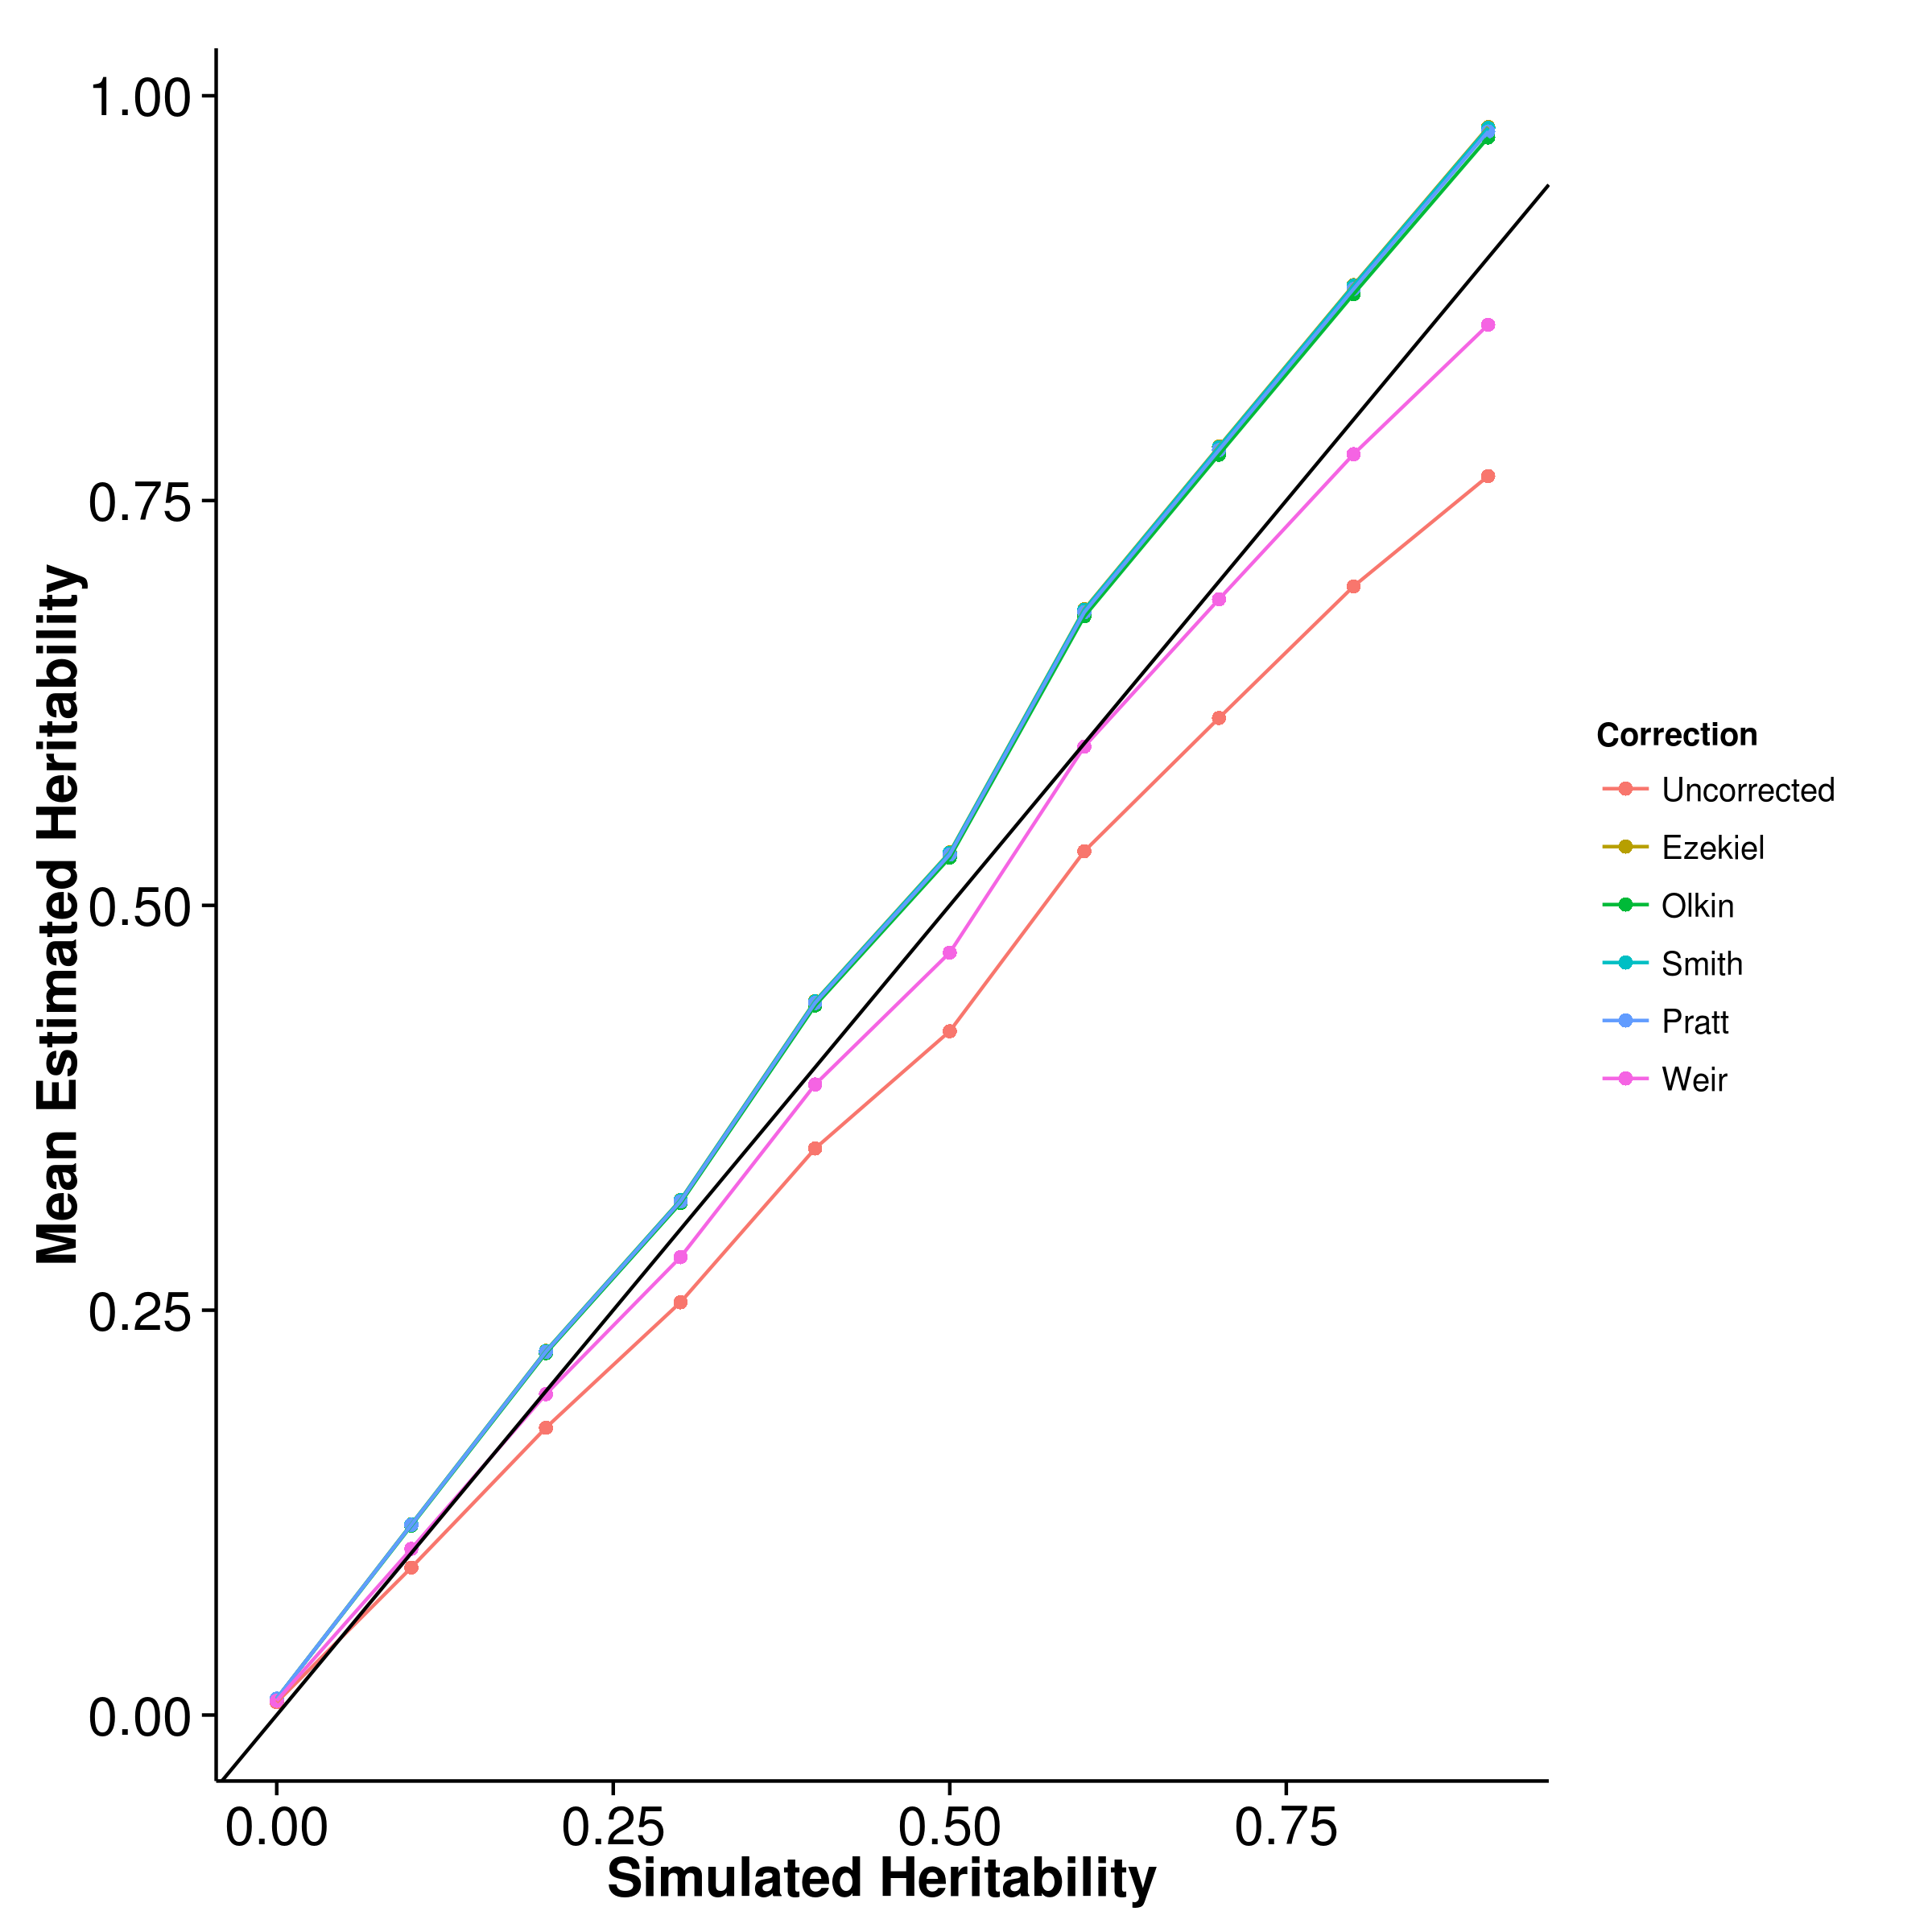
\includegraphics{figure/quantitative/ld_correct/ldCom_mean.png}}
				\label{fig:meanLDCor}
			}
			\subfloat[Empirical Variance]{
				\scalebox{.4}{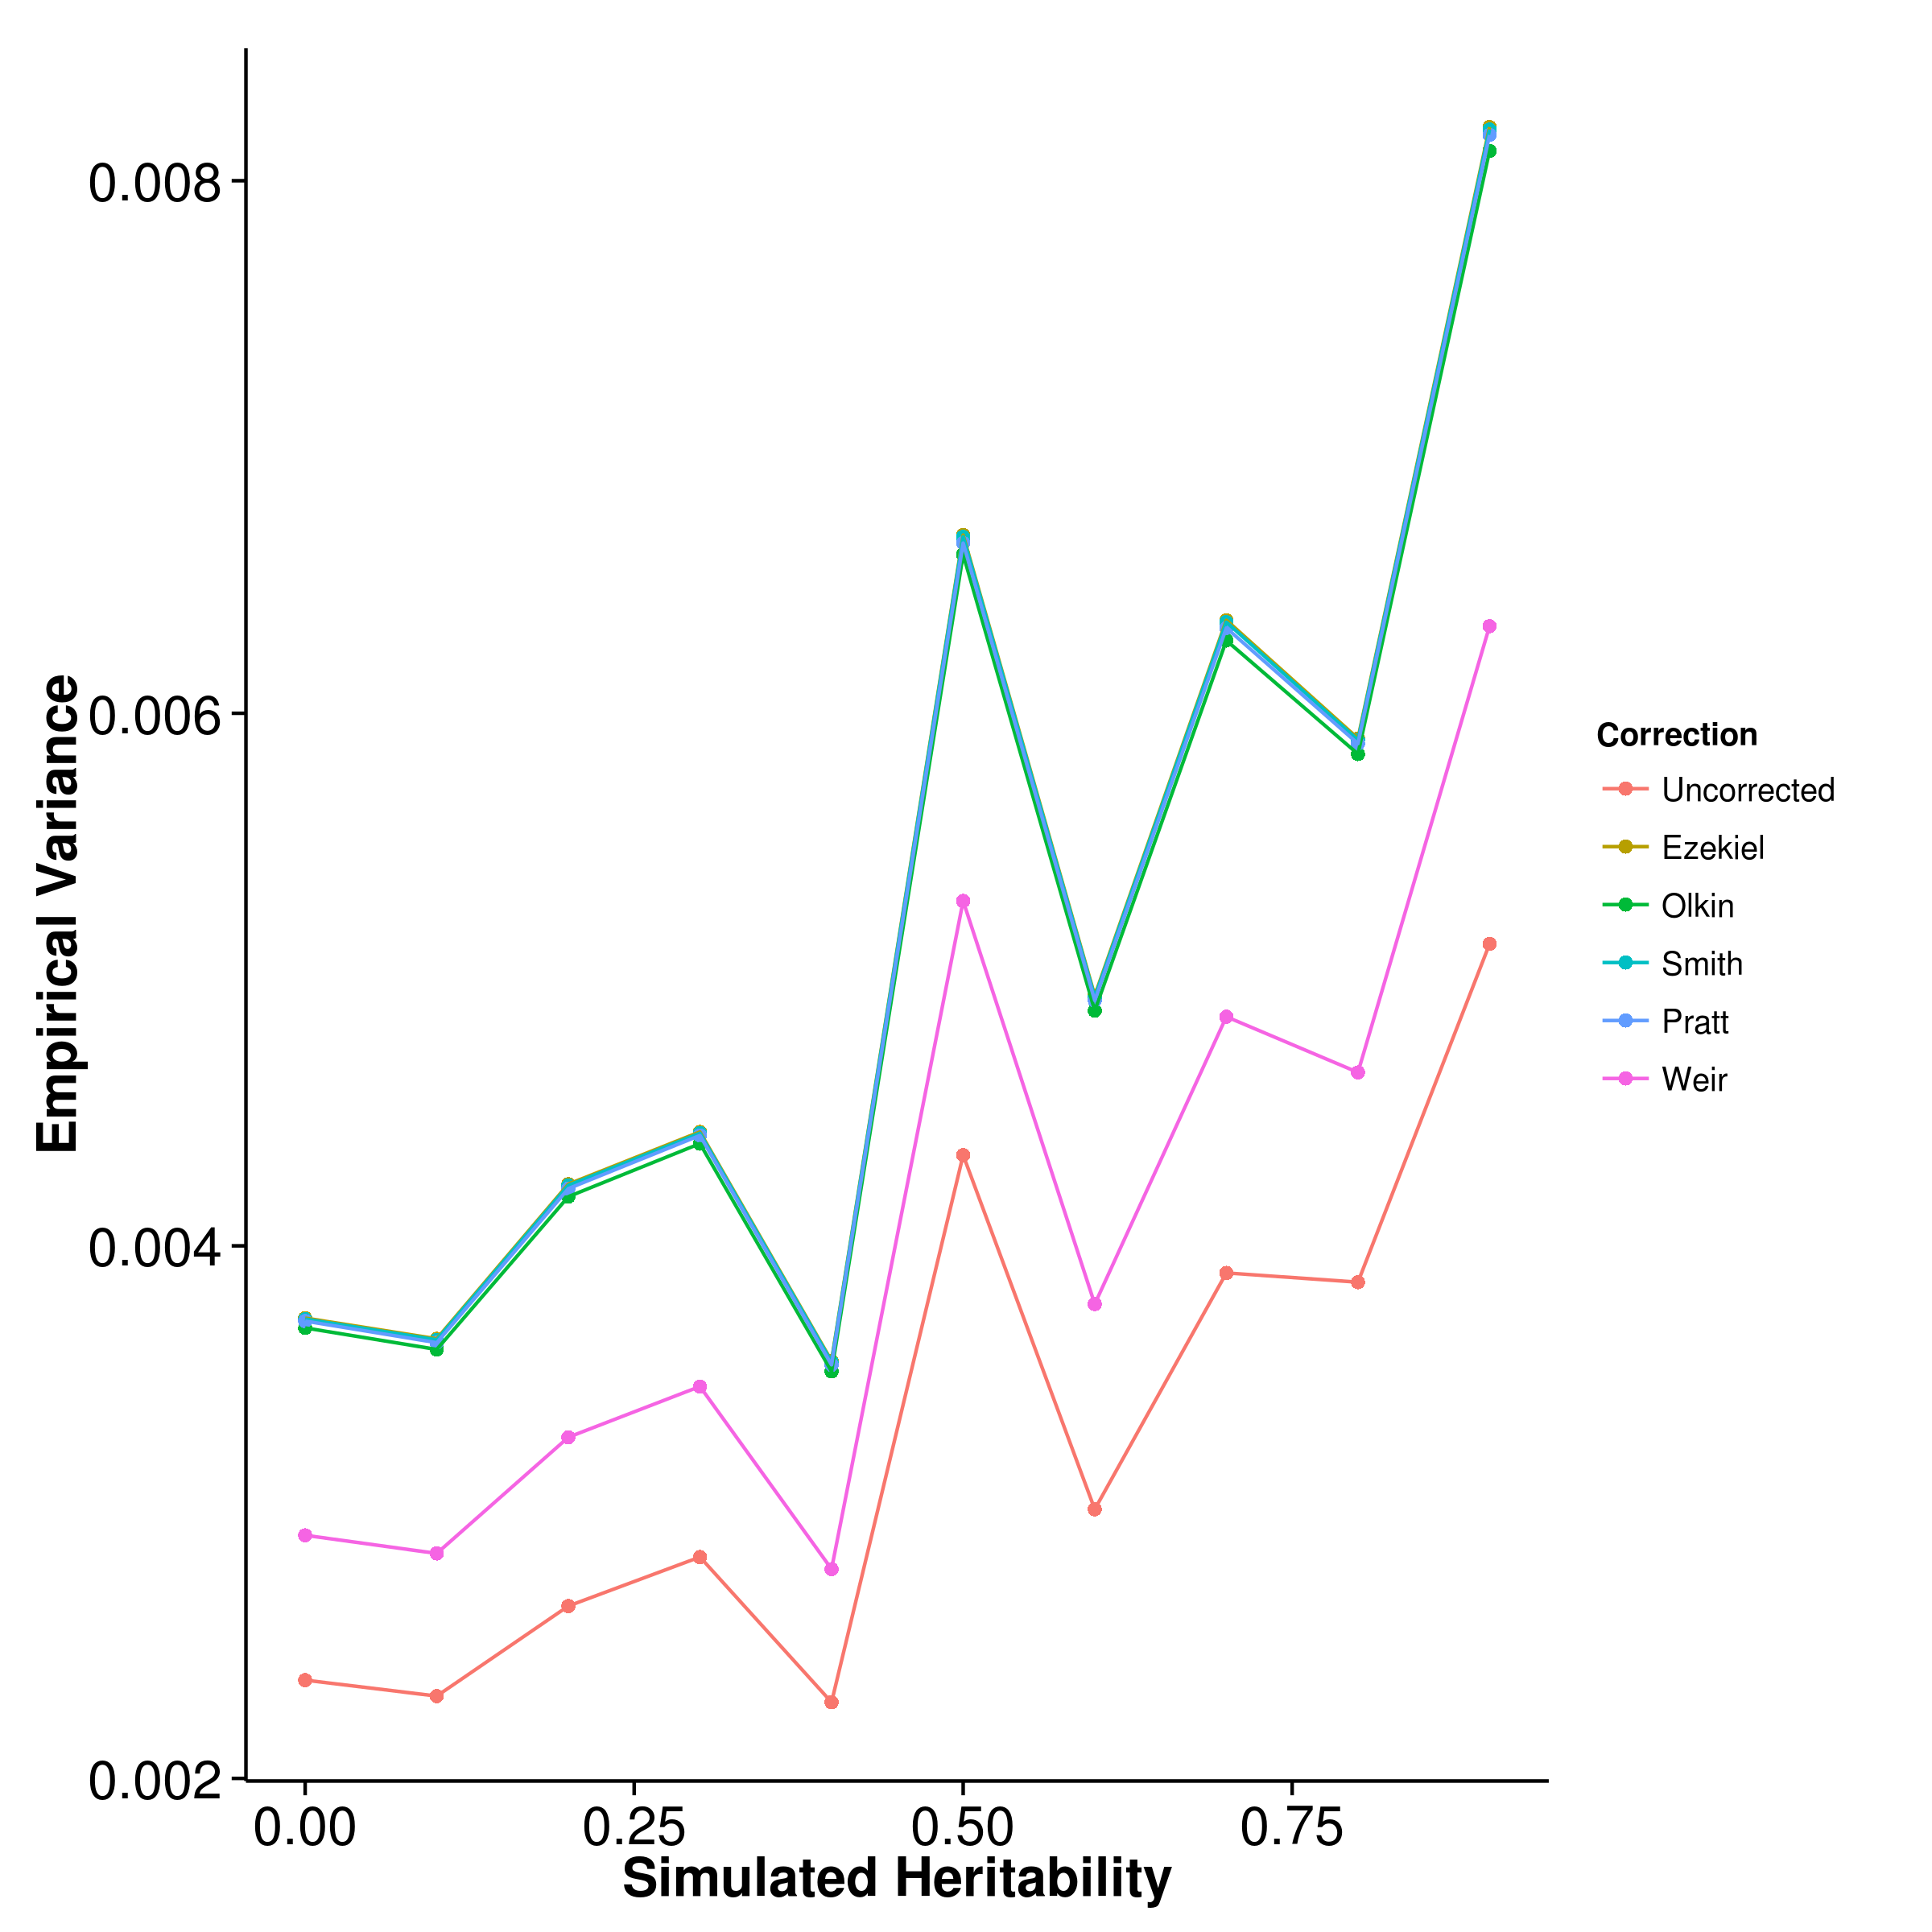
\includegraphics{figure/quantitative/ld_correct/ldCom_var.png}}
				\label{fig:varLDCor}
			}
			\caption[Effect of LD correction to Heritability Estimation]
			{Effect of LD correction to Heritability Estimation.
				We compared the performance of our algorithm when different $R^2$ bias correction algorithm was used.
				When no bias correction was carried out, a downward bias was observed. 
				After the application of the bias correction algorithms, the mean estimations of all except in the case of Weir \cref{eq:weir} algorithms leads to an overestimation of heritability.
				On the other hand, the corrections all lead to increase in variance of the estimation.
			} 
			\label{fig:ldCorCom}
		\end{figure}
		First, we would like to assess the effect of \gls{LD} correction on the heritability estimation and the impact of different bias correction algorithms. 
		By performing the simulation using HAPGEN2, we were able to simulate sample with \gls{LD} structure comparable to the \gls{LD} of the 1000 genome \gls{CEU} samples.
		
		First, we would like to compare the performance of \gls{shrek} when different bias correction algorithms were applied (\cref{fig:meanLDCor}).
		From the graph, it was observed that when no bias correction was applied, the mean estimation were in general downwardly biased.
		This was consistent with our expectation of a general upward bias in sample $R^2$ which will downwardly penalize the resulting heritability estimation.
		On the other hand, the bias correction algorithms all worked as expected where they increases the mean estimation of heritability.
		By removing the upward bias in the sample $R^2$, the heritability estimation should increase.
		However for most algorithms except for Weir's formula (\cref{eq:weir}) an over adjustment were observed, leading to a general upward bias in the estimation.
		Taking into account of the variance of estimation (\cref{fig:varLDCor}), Weir's formula were the most suitable for \gls{shrek} where not only it reduces the bias in the final heritability estimation, it does not introduce too much additional variance into the estimation.
		As a result of that, we selected the Weir's formula as our default \gls{LD} correction algorithm.
		
		\subsection{Comparing with Other Algorithms}
		Having selected the optimal \gls{LD} correction algorithm, we then compared the performance of \gls{shrek} with existing algorithms to understand the relative of these algorithms under different conditions.
		First, we examined the performance of the algorithms under the quantitative trait scenario where we varies the trait heritability and the number of causal \glspl{SNP}.
		
		\subsubsection{Quantitative Trait Simulation}
			\begin{figure}
			\centering
			\subfloat[SHREK]{
				\scalebox{.4}{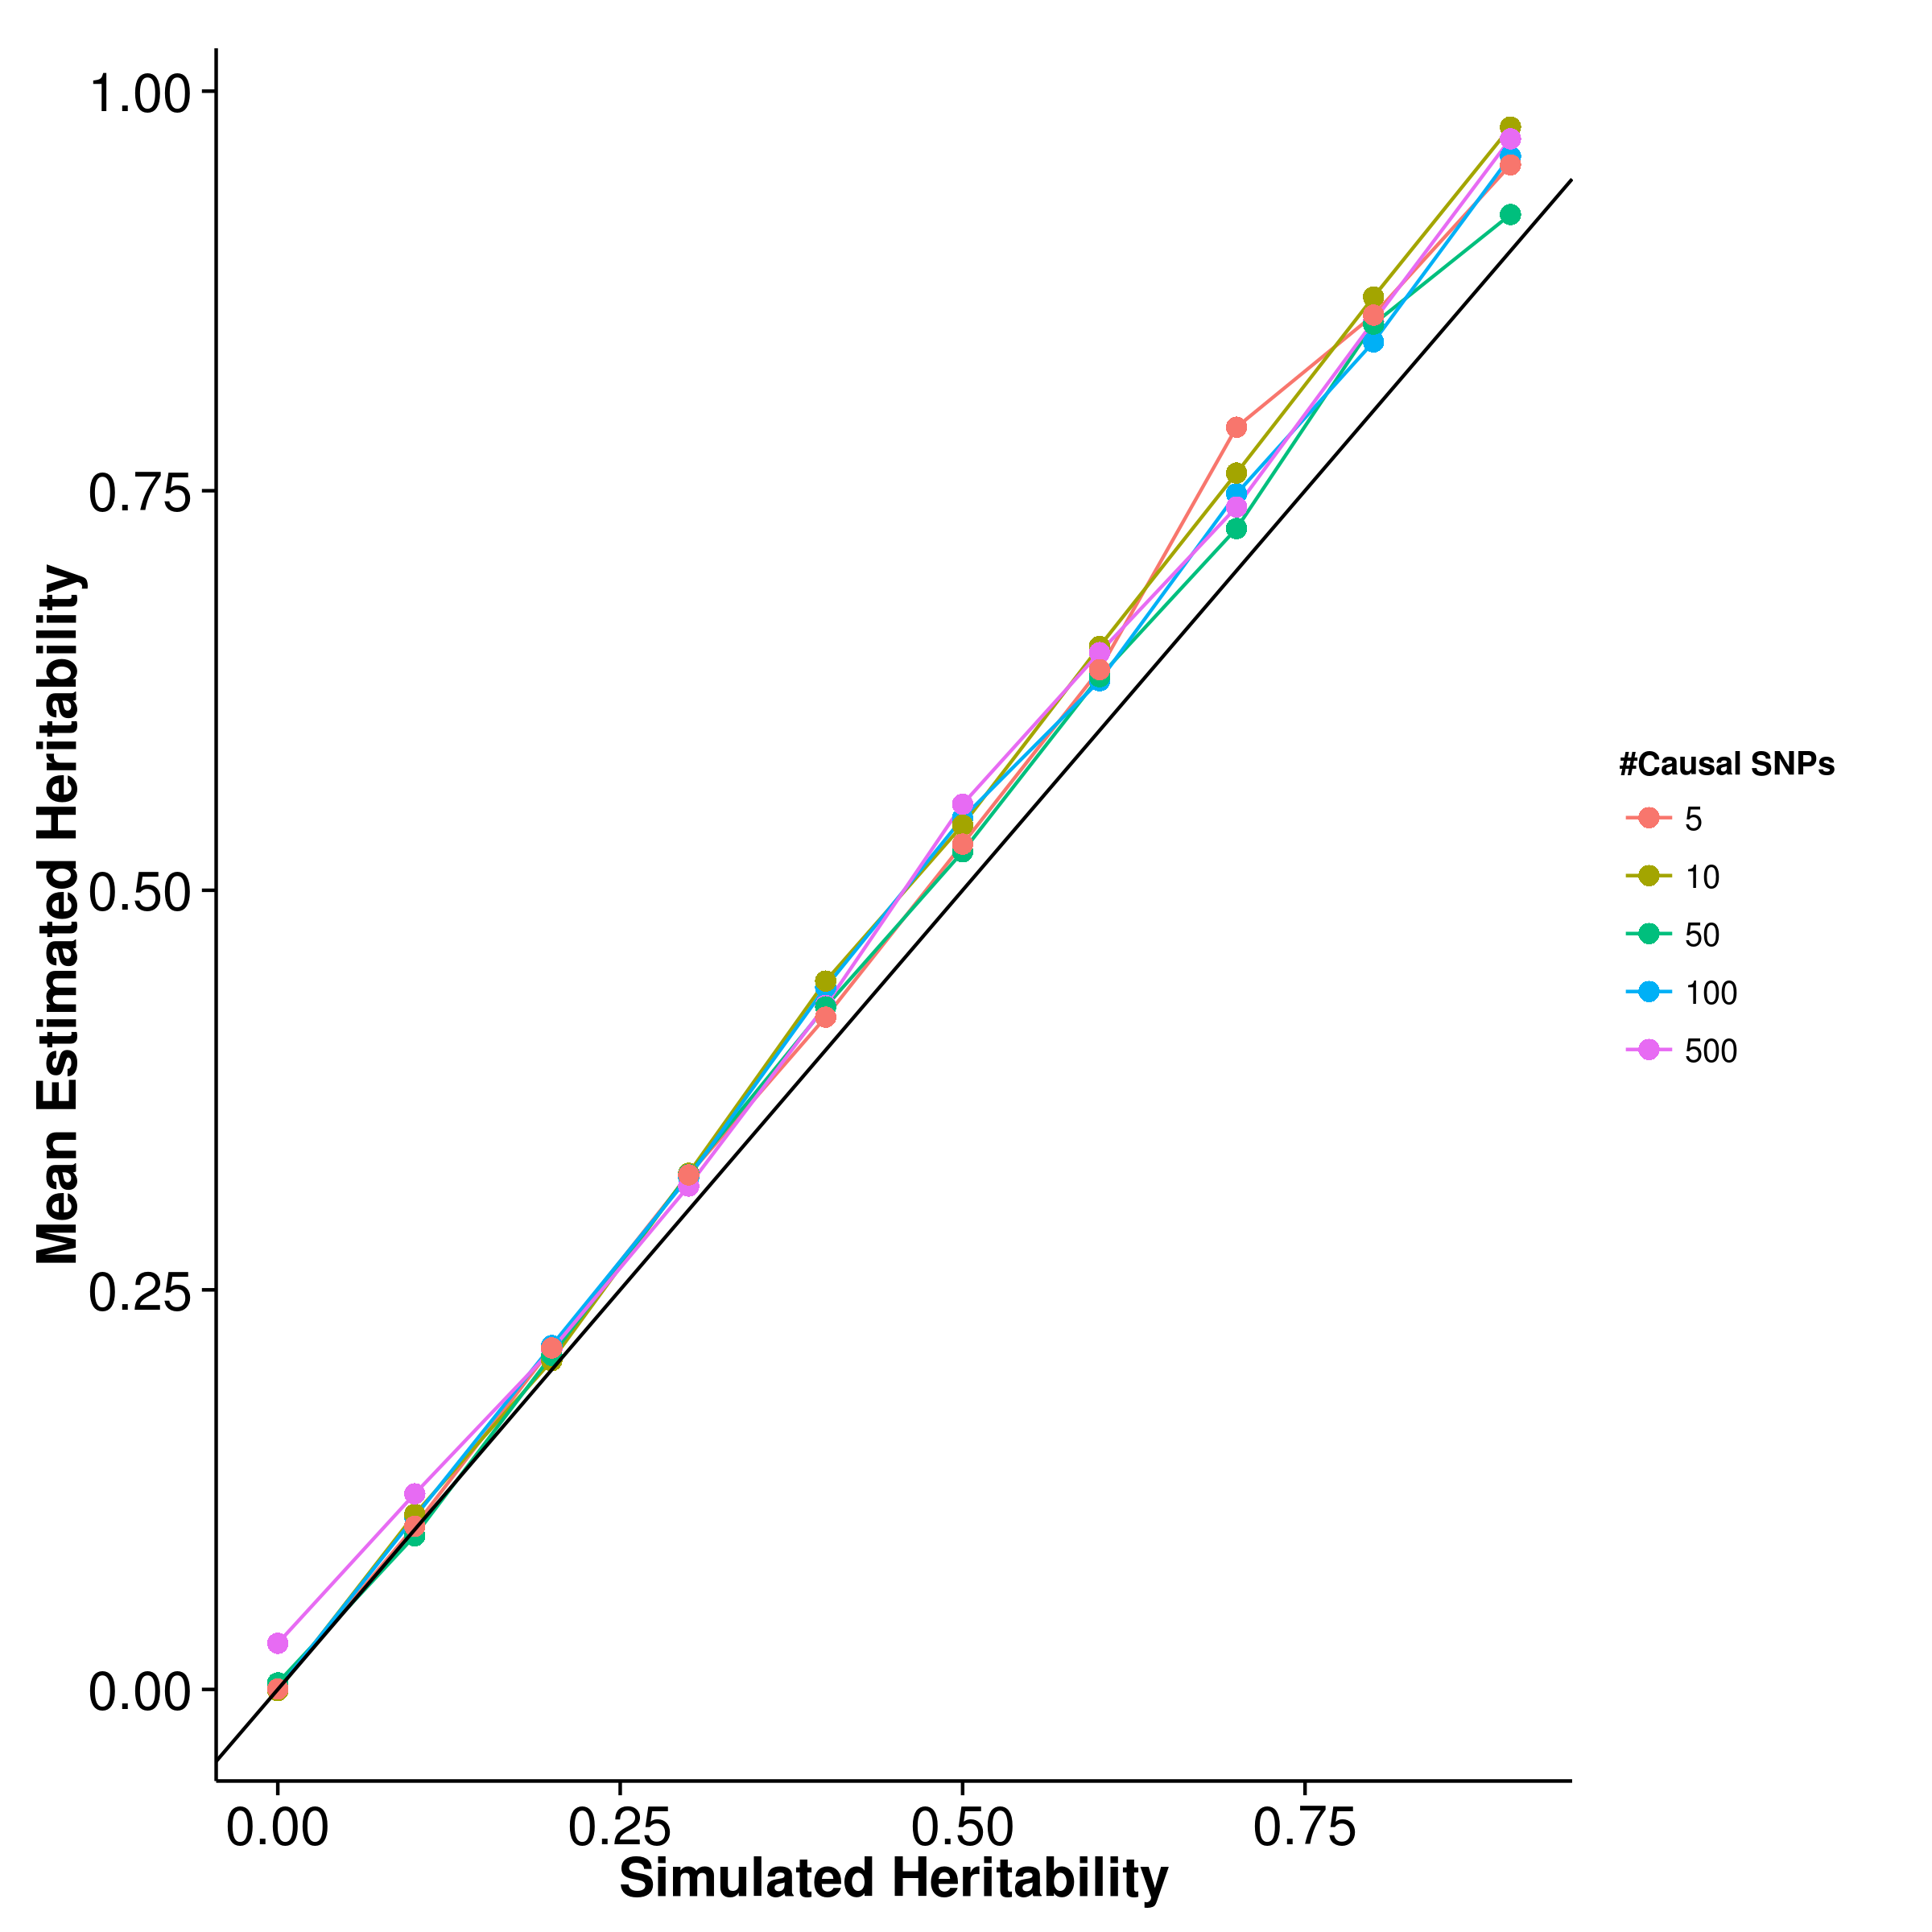
\includegraphics{figure/he_summary/random/shrek_Qt_Rand_mean.png}}
				\label{fig:shrekQtRandMean}
			}
			\subfloat[GCTA]{
				\scalebox{.4}{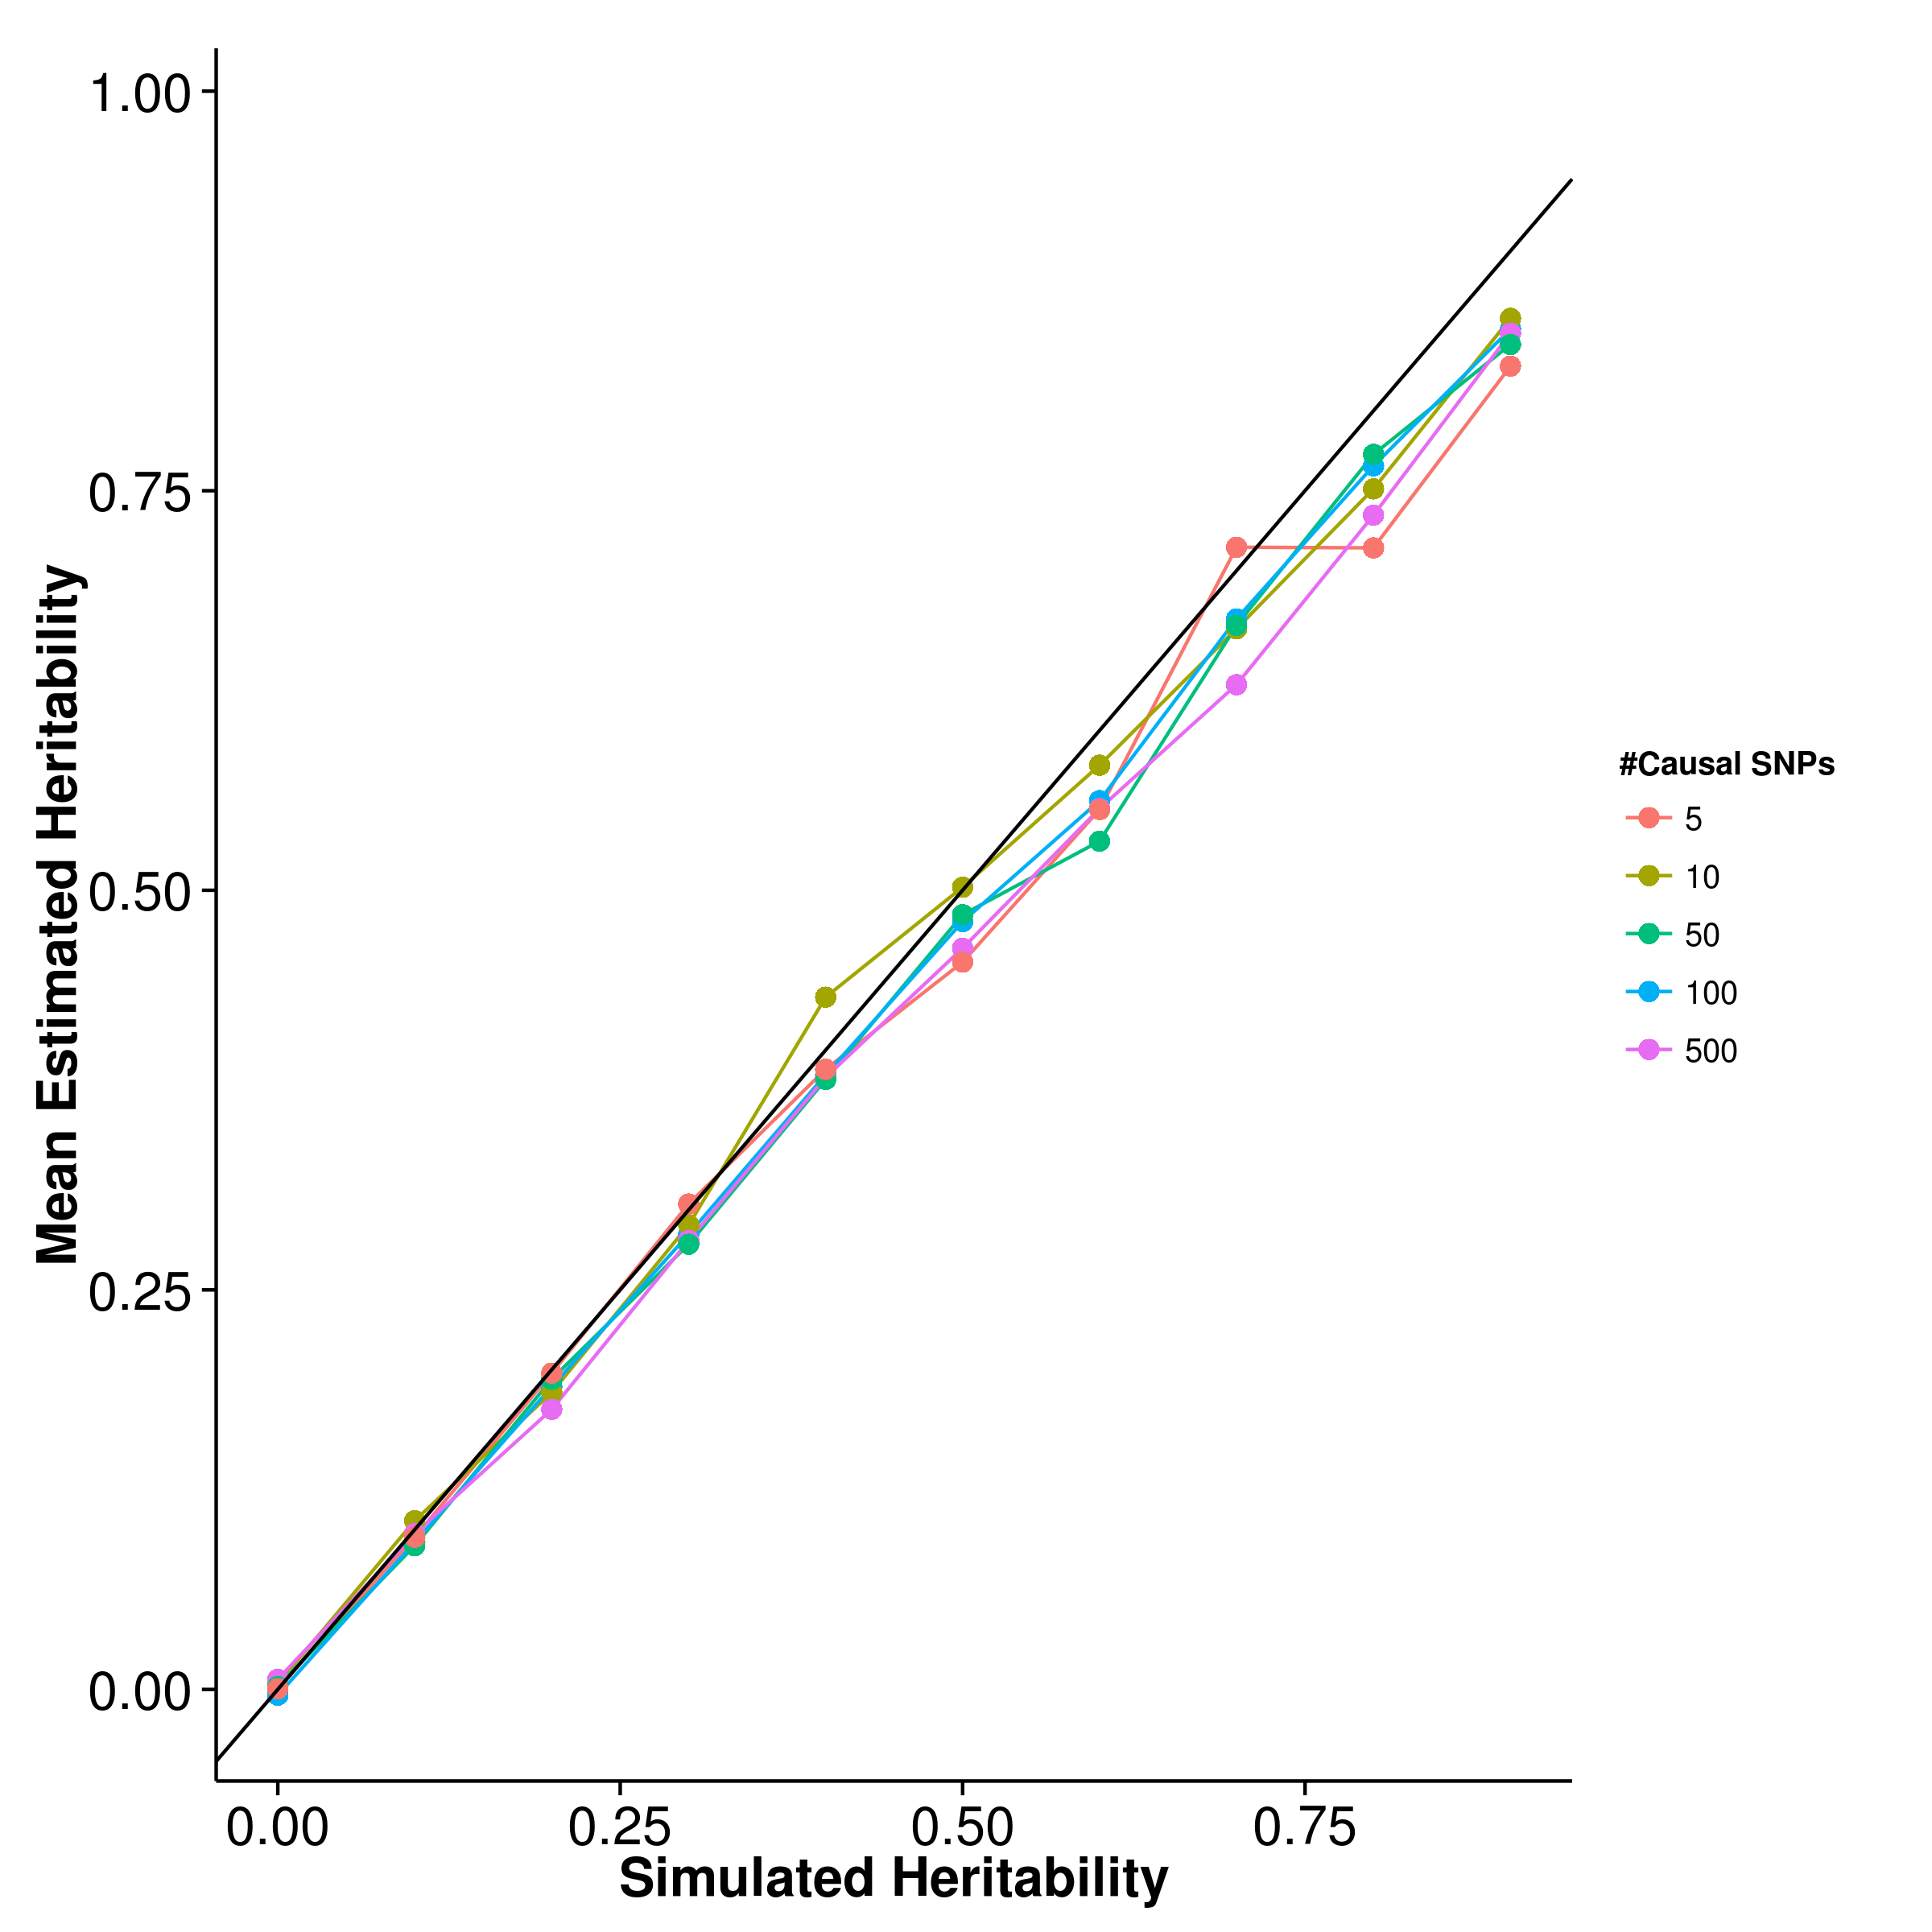
\includegraphics{figure/he_summary/random/gcta_Qt_Rand_mean.png}}
				\label{fig:gctaQtRandMean}
			}\\
			\subfloat[LDSC with fix intercept]{
				\scalebox{.4}{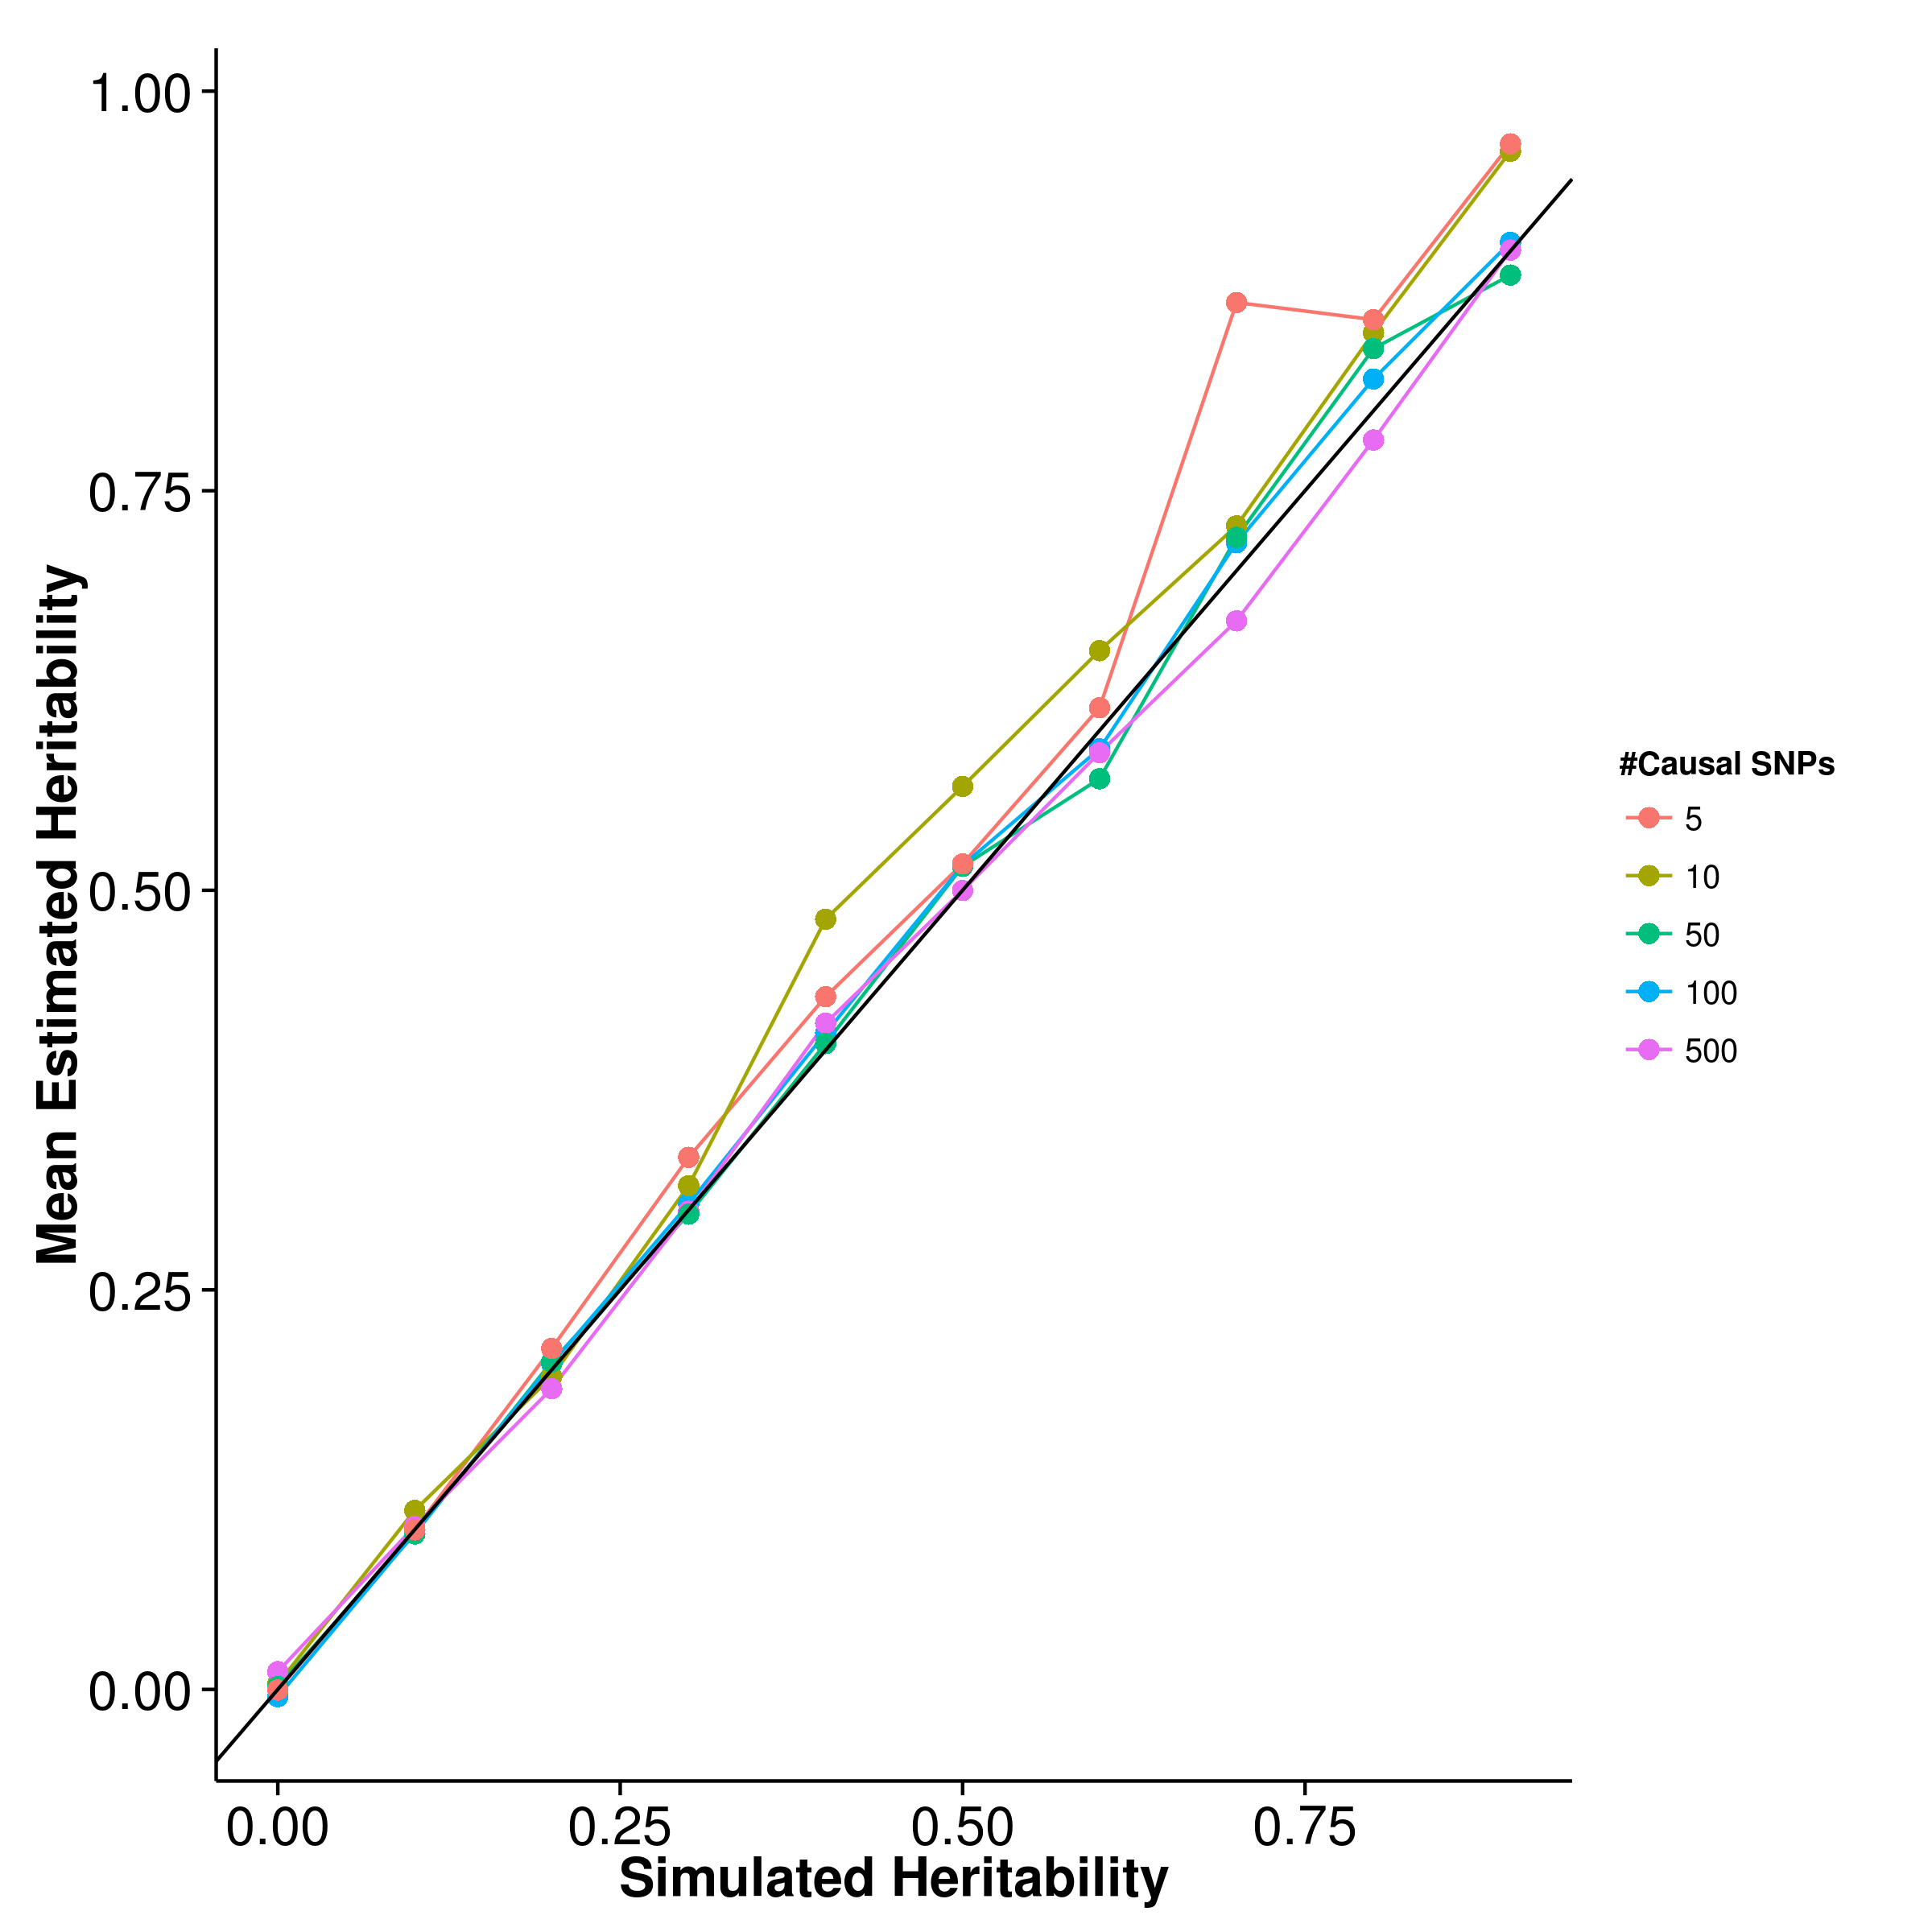
\includegraphics{figure/he_summary/random/ldsc_Qt_Rand_mean.png}}
				\label{fig:ldscQtRandMean}
			}
			\subfloat[LDSC with intercept estimation]{
				
				\scalebox{.4}{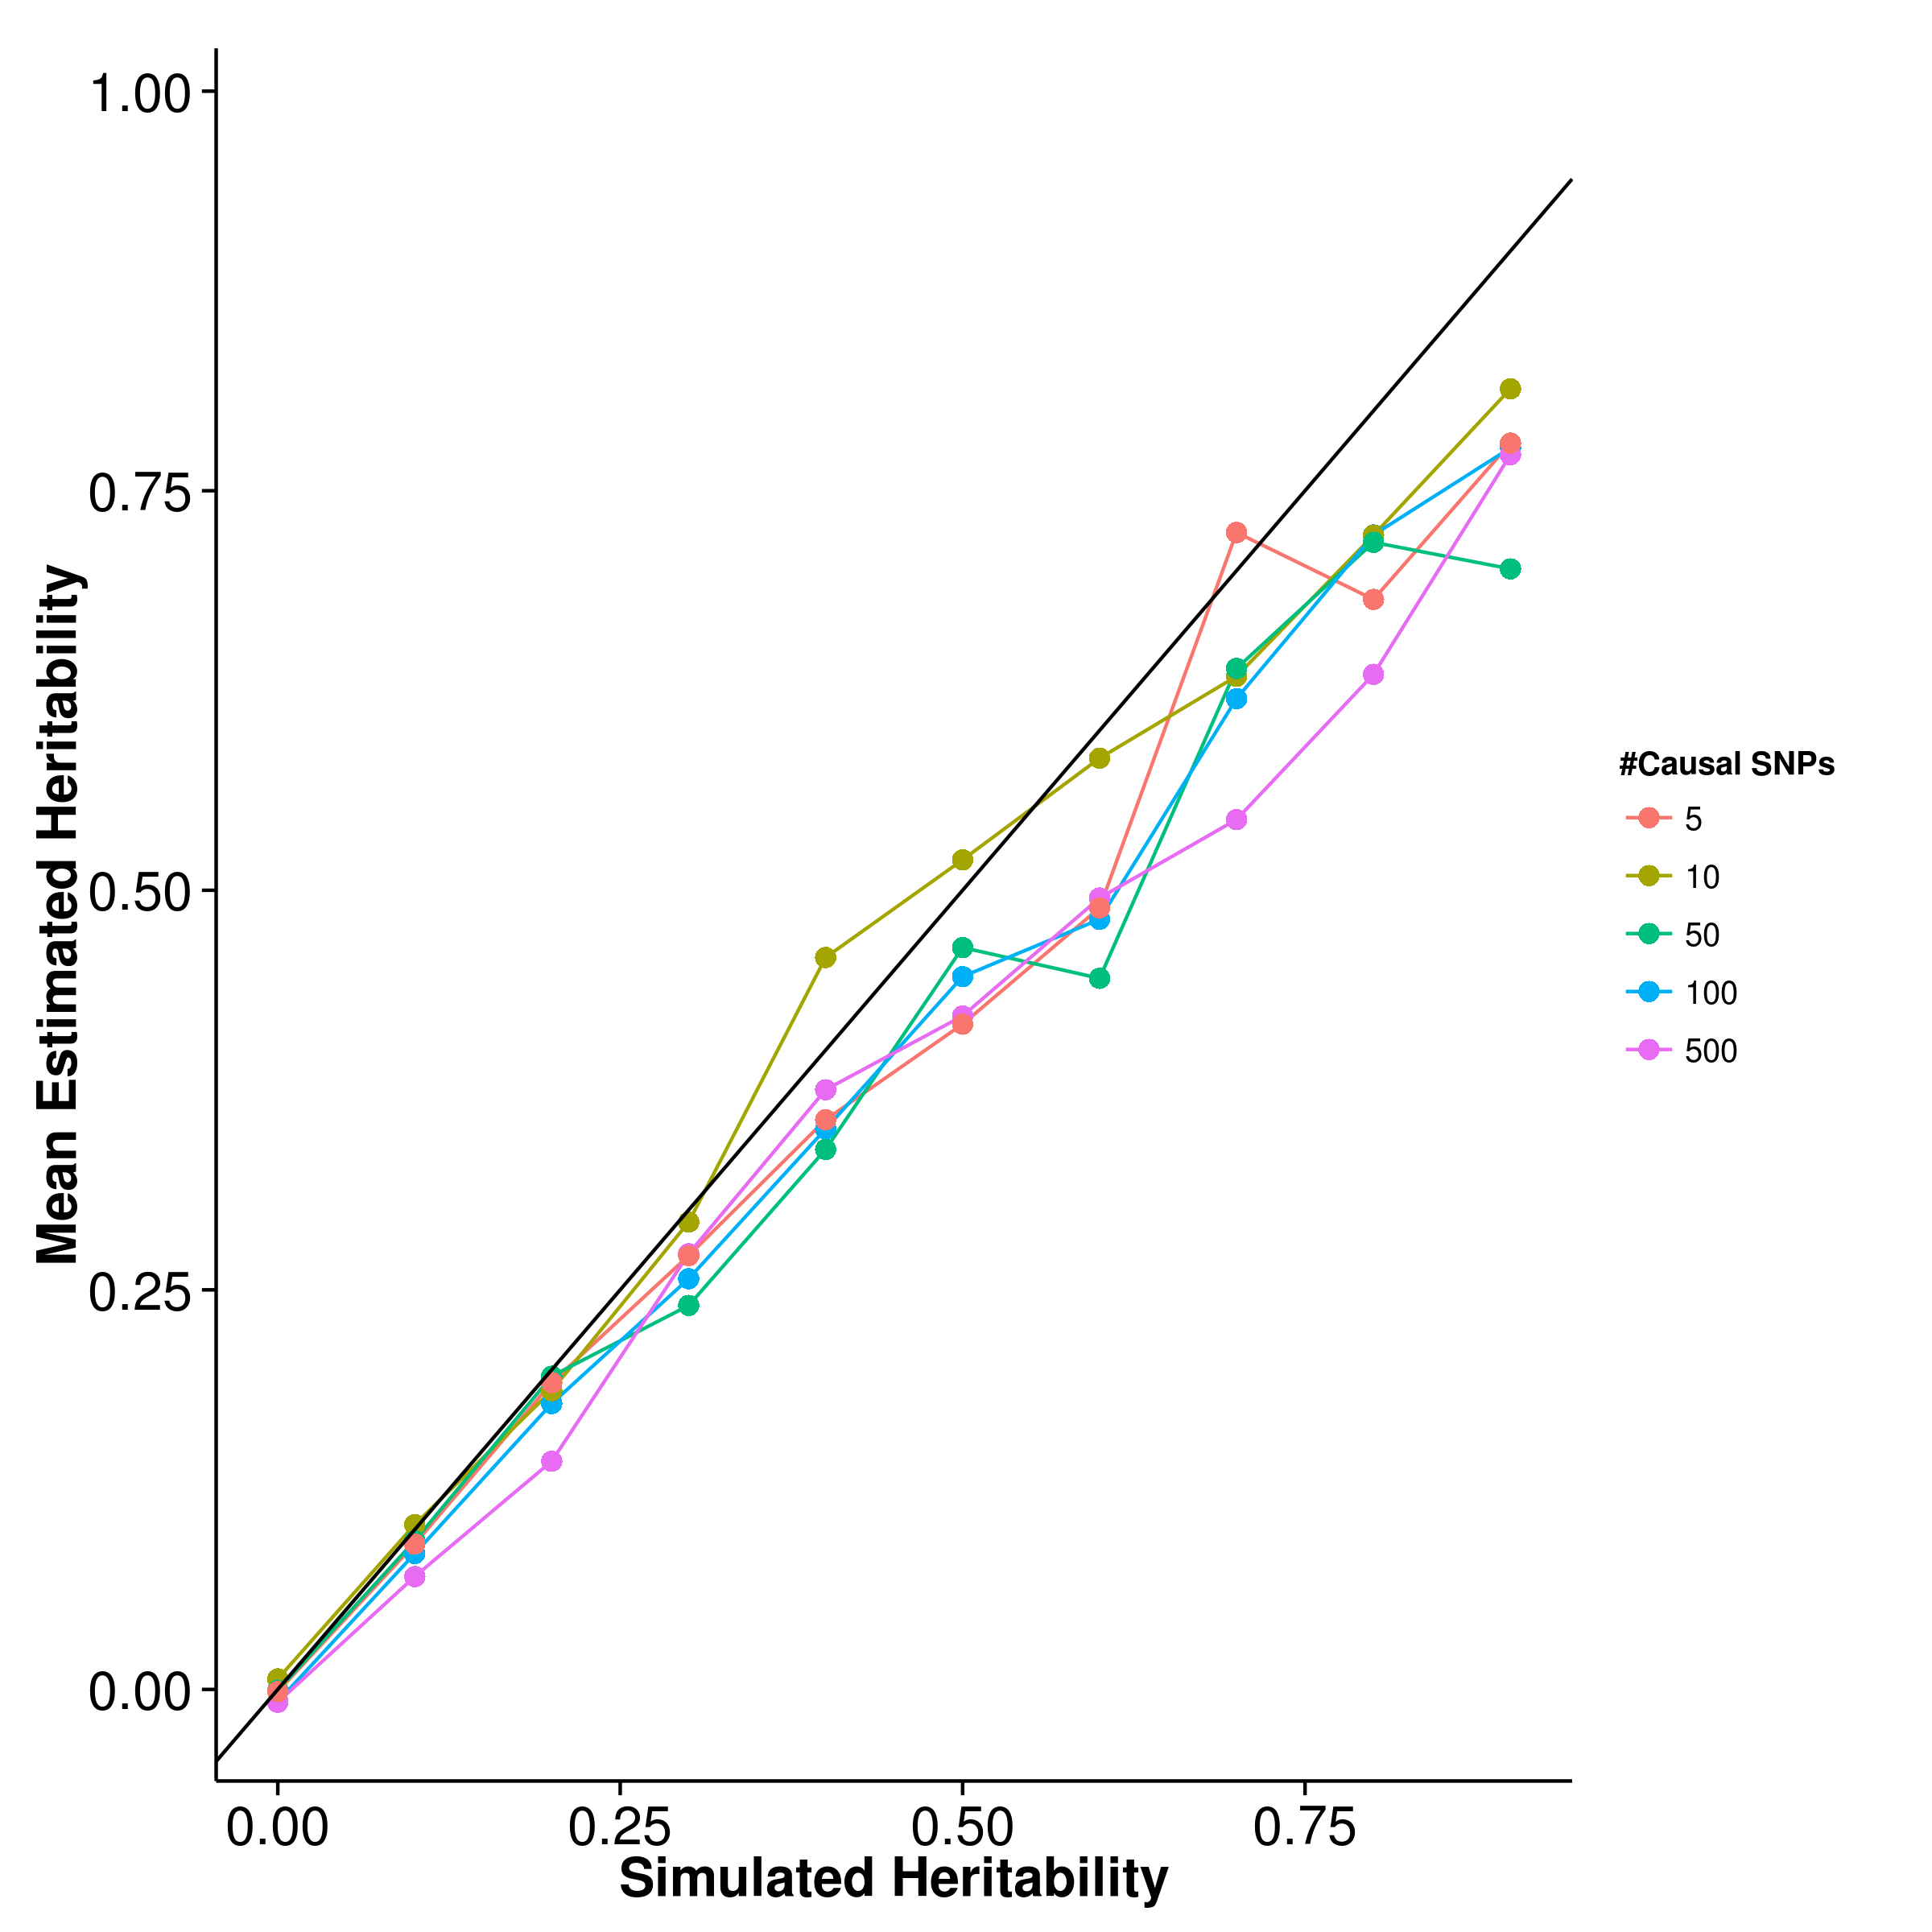
\includegraphics{figure/he_summary/random/ldscIn_Qt_Rand_mean.png}}
				\label{fig:ldscInQtRandMean}
			}
			\caption[Mean of Quantitative Trait Simulation Results]
			{Mean of results from quantitative trait simulation with random effect size simulation.
				Estimations form \gls{shrek} were slightly biased upwards whereas \gls{gcta} and \gls{ldsc} with intercept estimations both biased downwards.
				On the other hand, \gls{ldsc} with fixed intercept provides least biased estimates under polygenic conditions. 
				However, when the number of causal \glspl{SNP} is small (e.g. 5 or 10), an upward bias was observed.} 
			\label{fig:QtRandMean}
		\end{figure}
		
		\begin{figure}
			\centering
			\subfloat[SHREK]{
				\scalebox{.4}{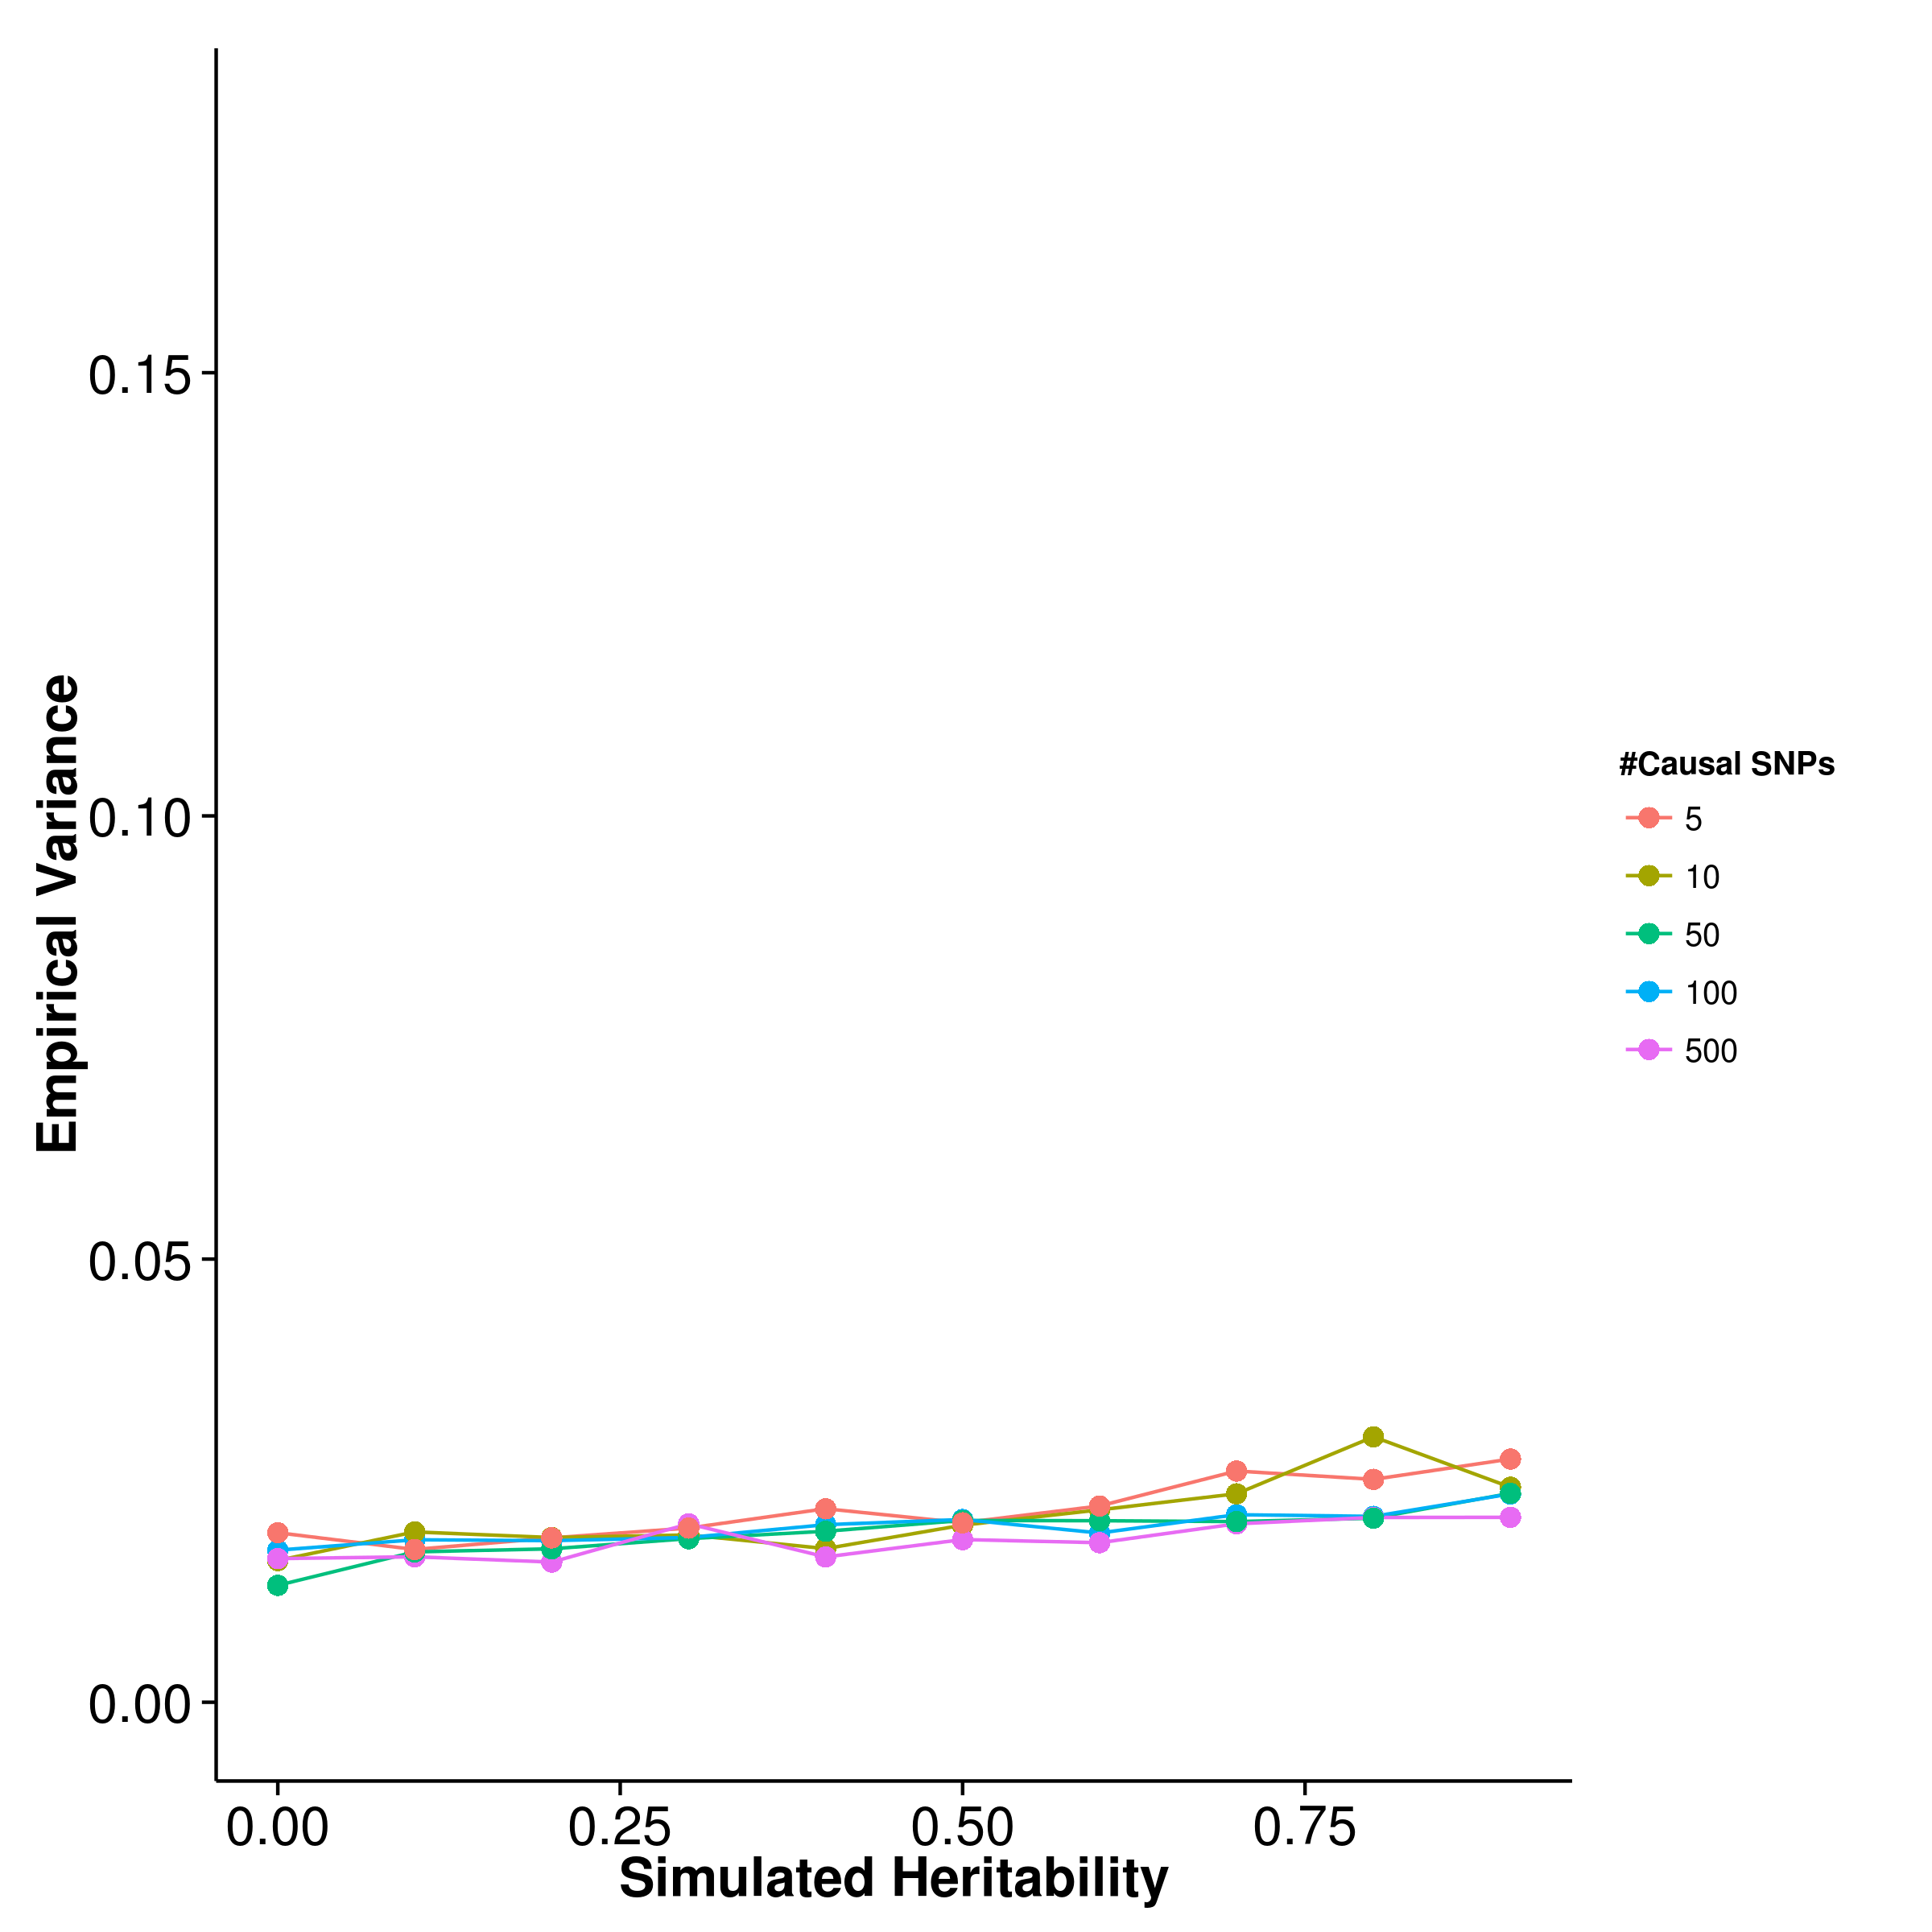
\includegraphics{figure/he_summary/random/shrek_Qt_Rand_sd.png}}
				\label{fig:shrekQtRandVar}
			}
			\subfloat[GCTA]{
				\scalebox{.4}{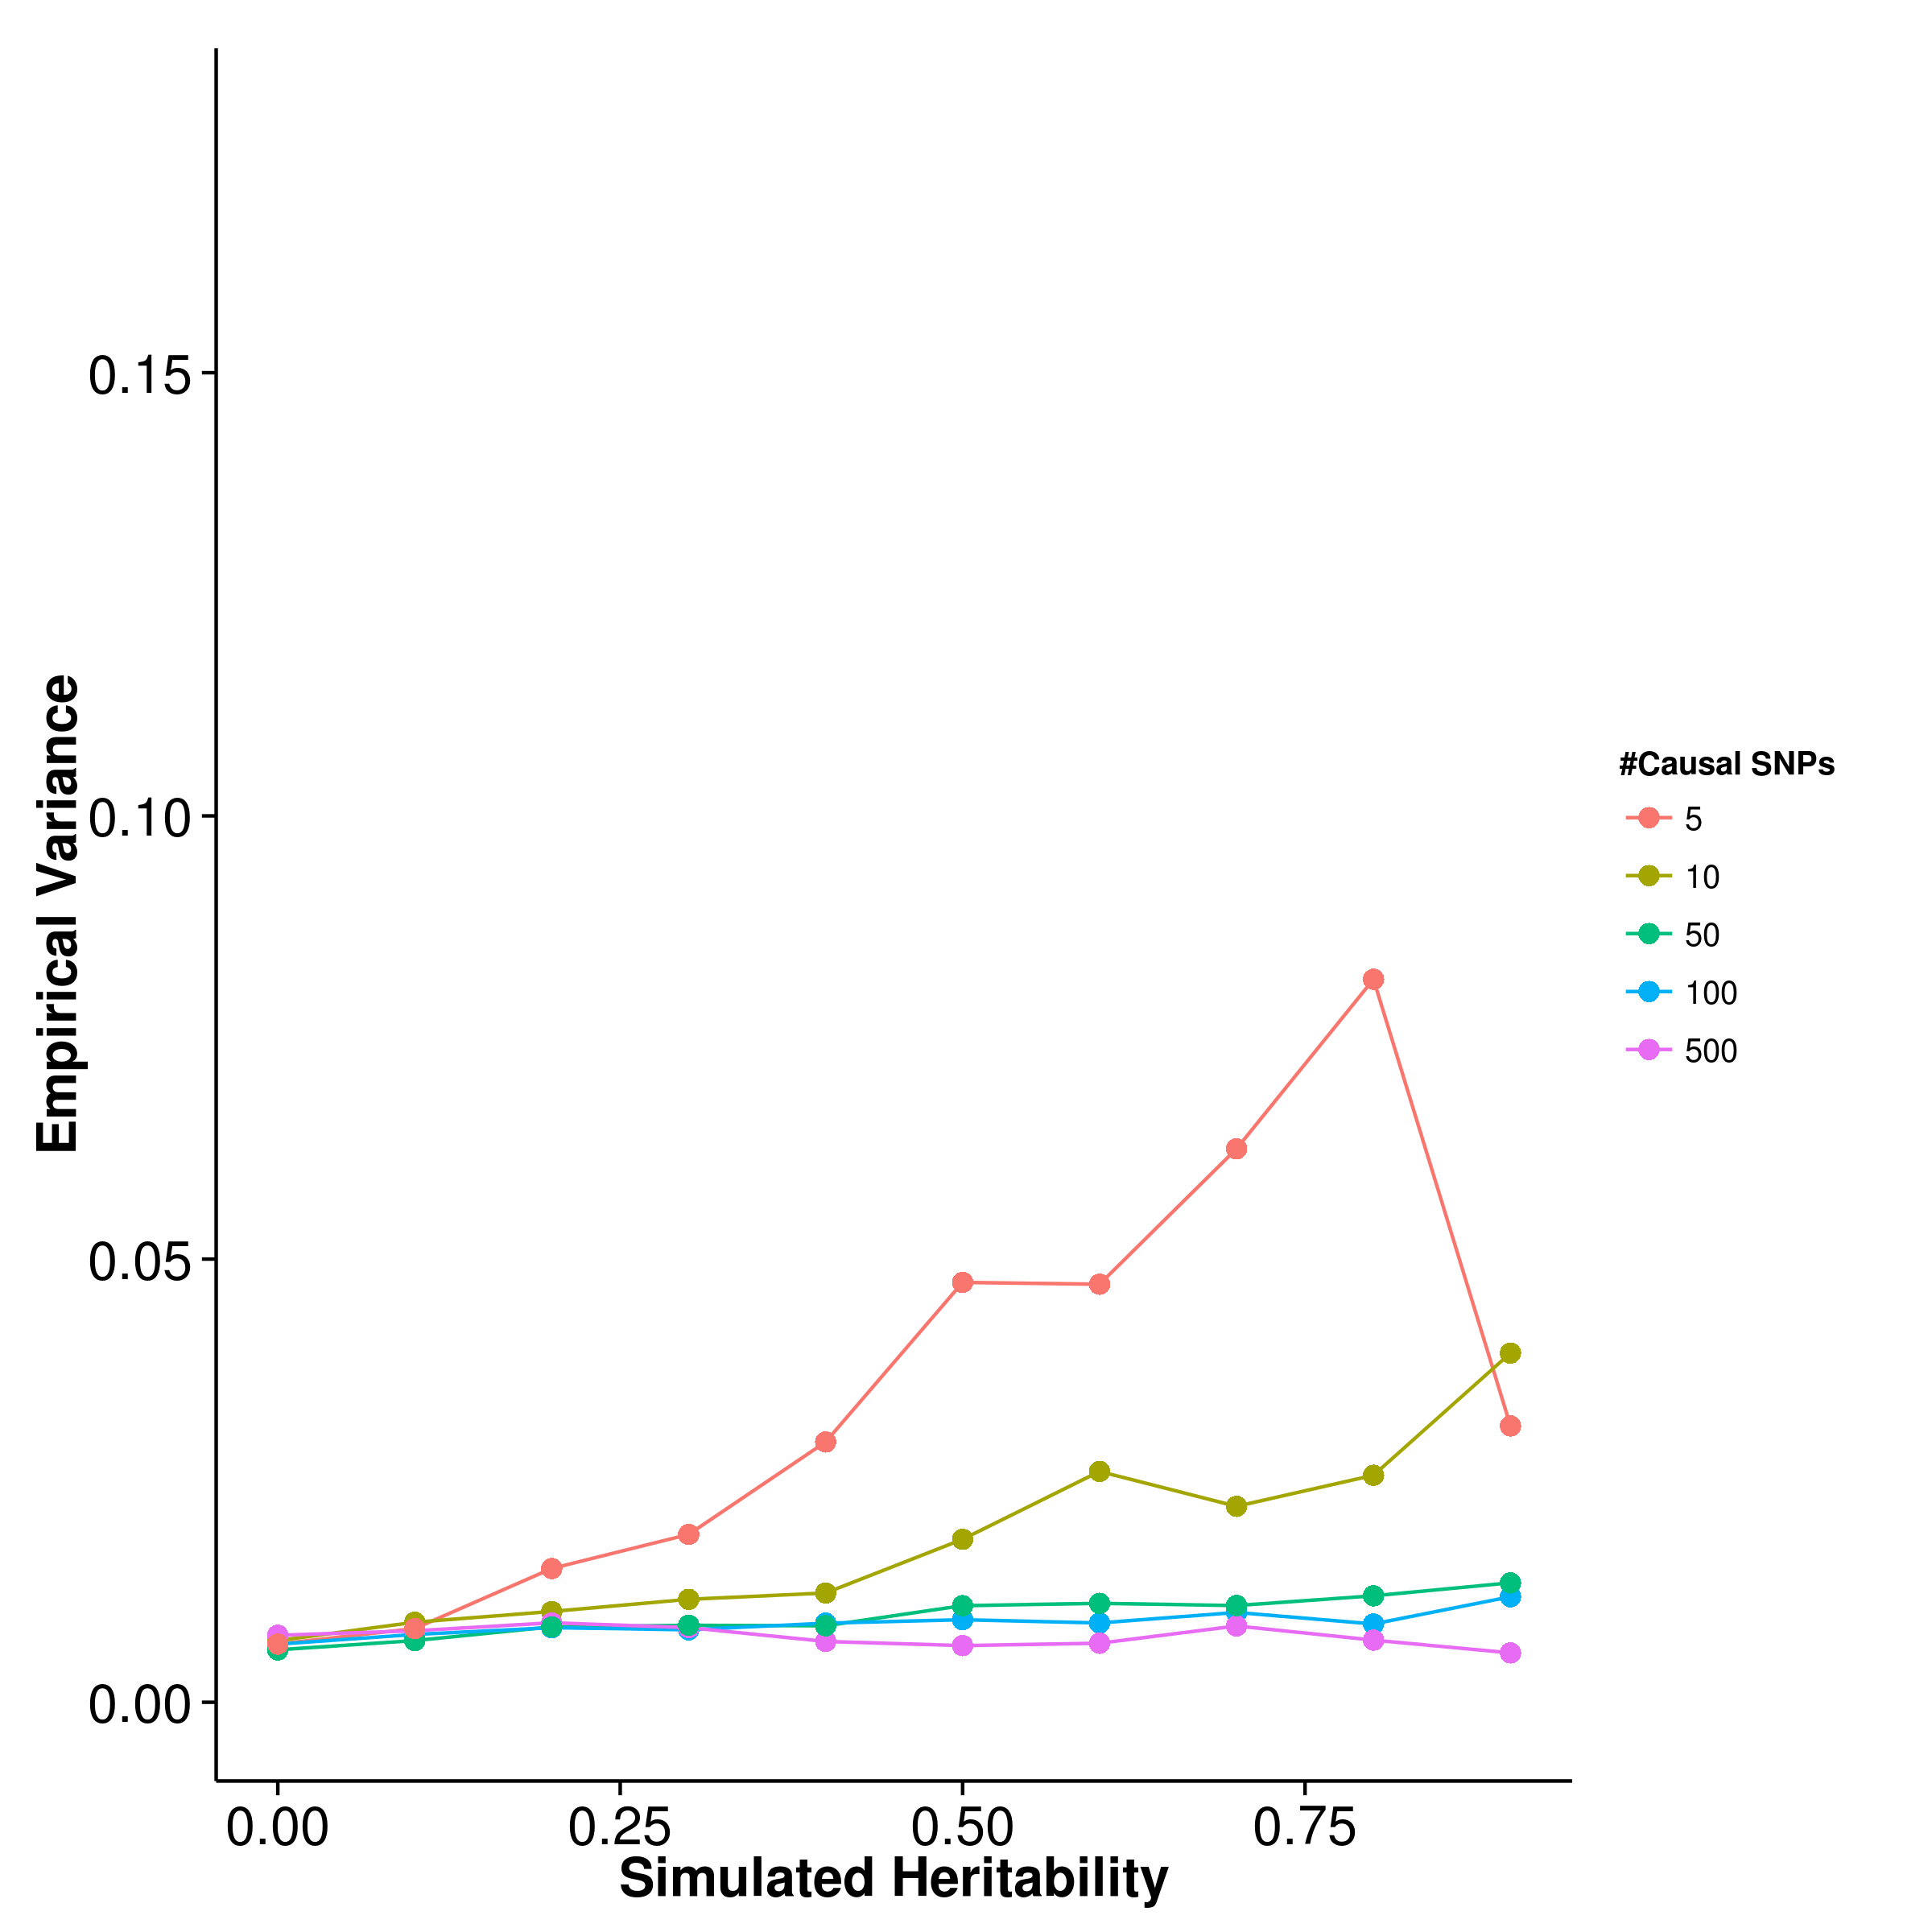
\includegraphics{figure/he_summary/random/gcta_Qt_Rand_sd.png}}
				\label{fig:gctaQtRandVar}
			}\\
			\subfloat[LDSC with fix intercept]{
				\scalebox{.4}{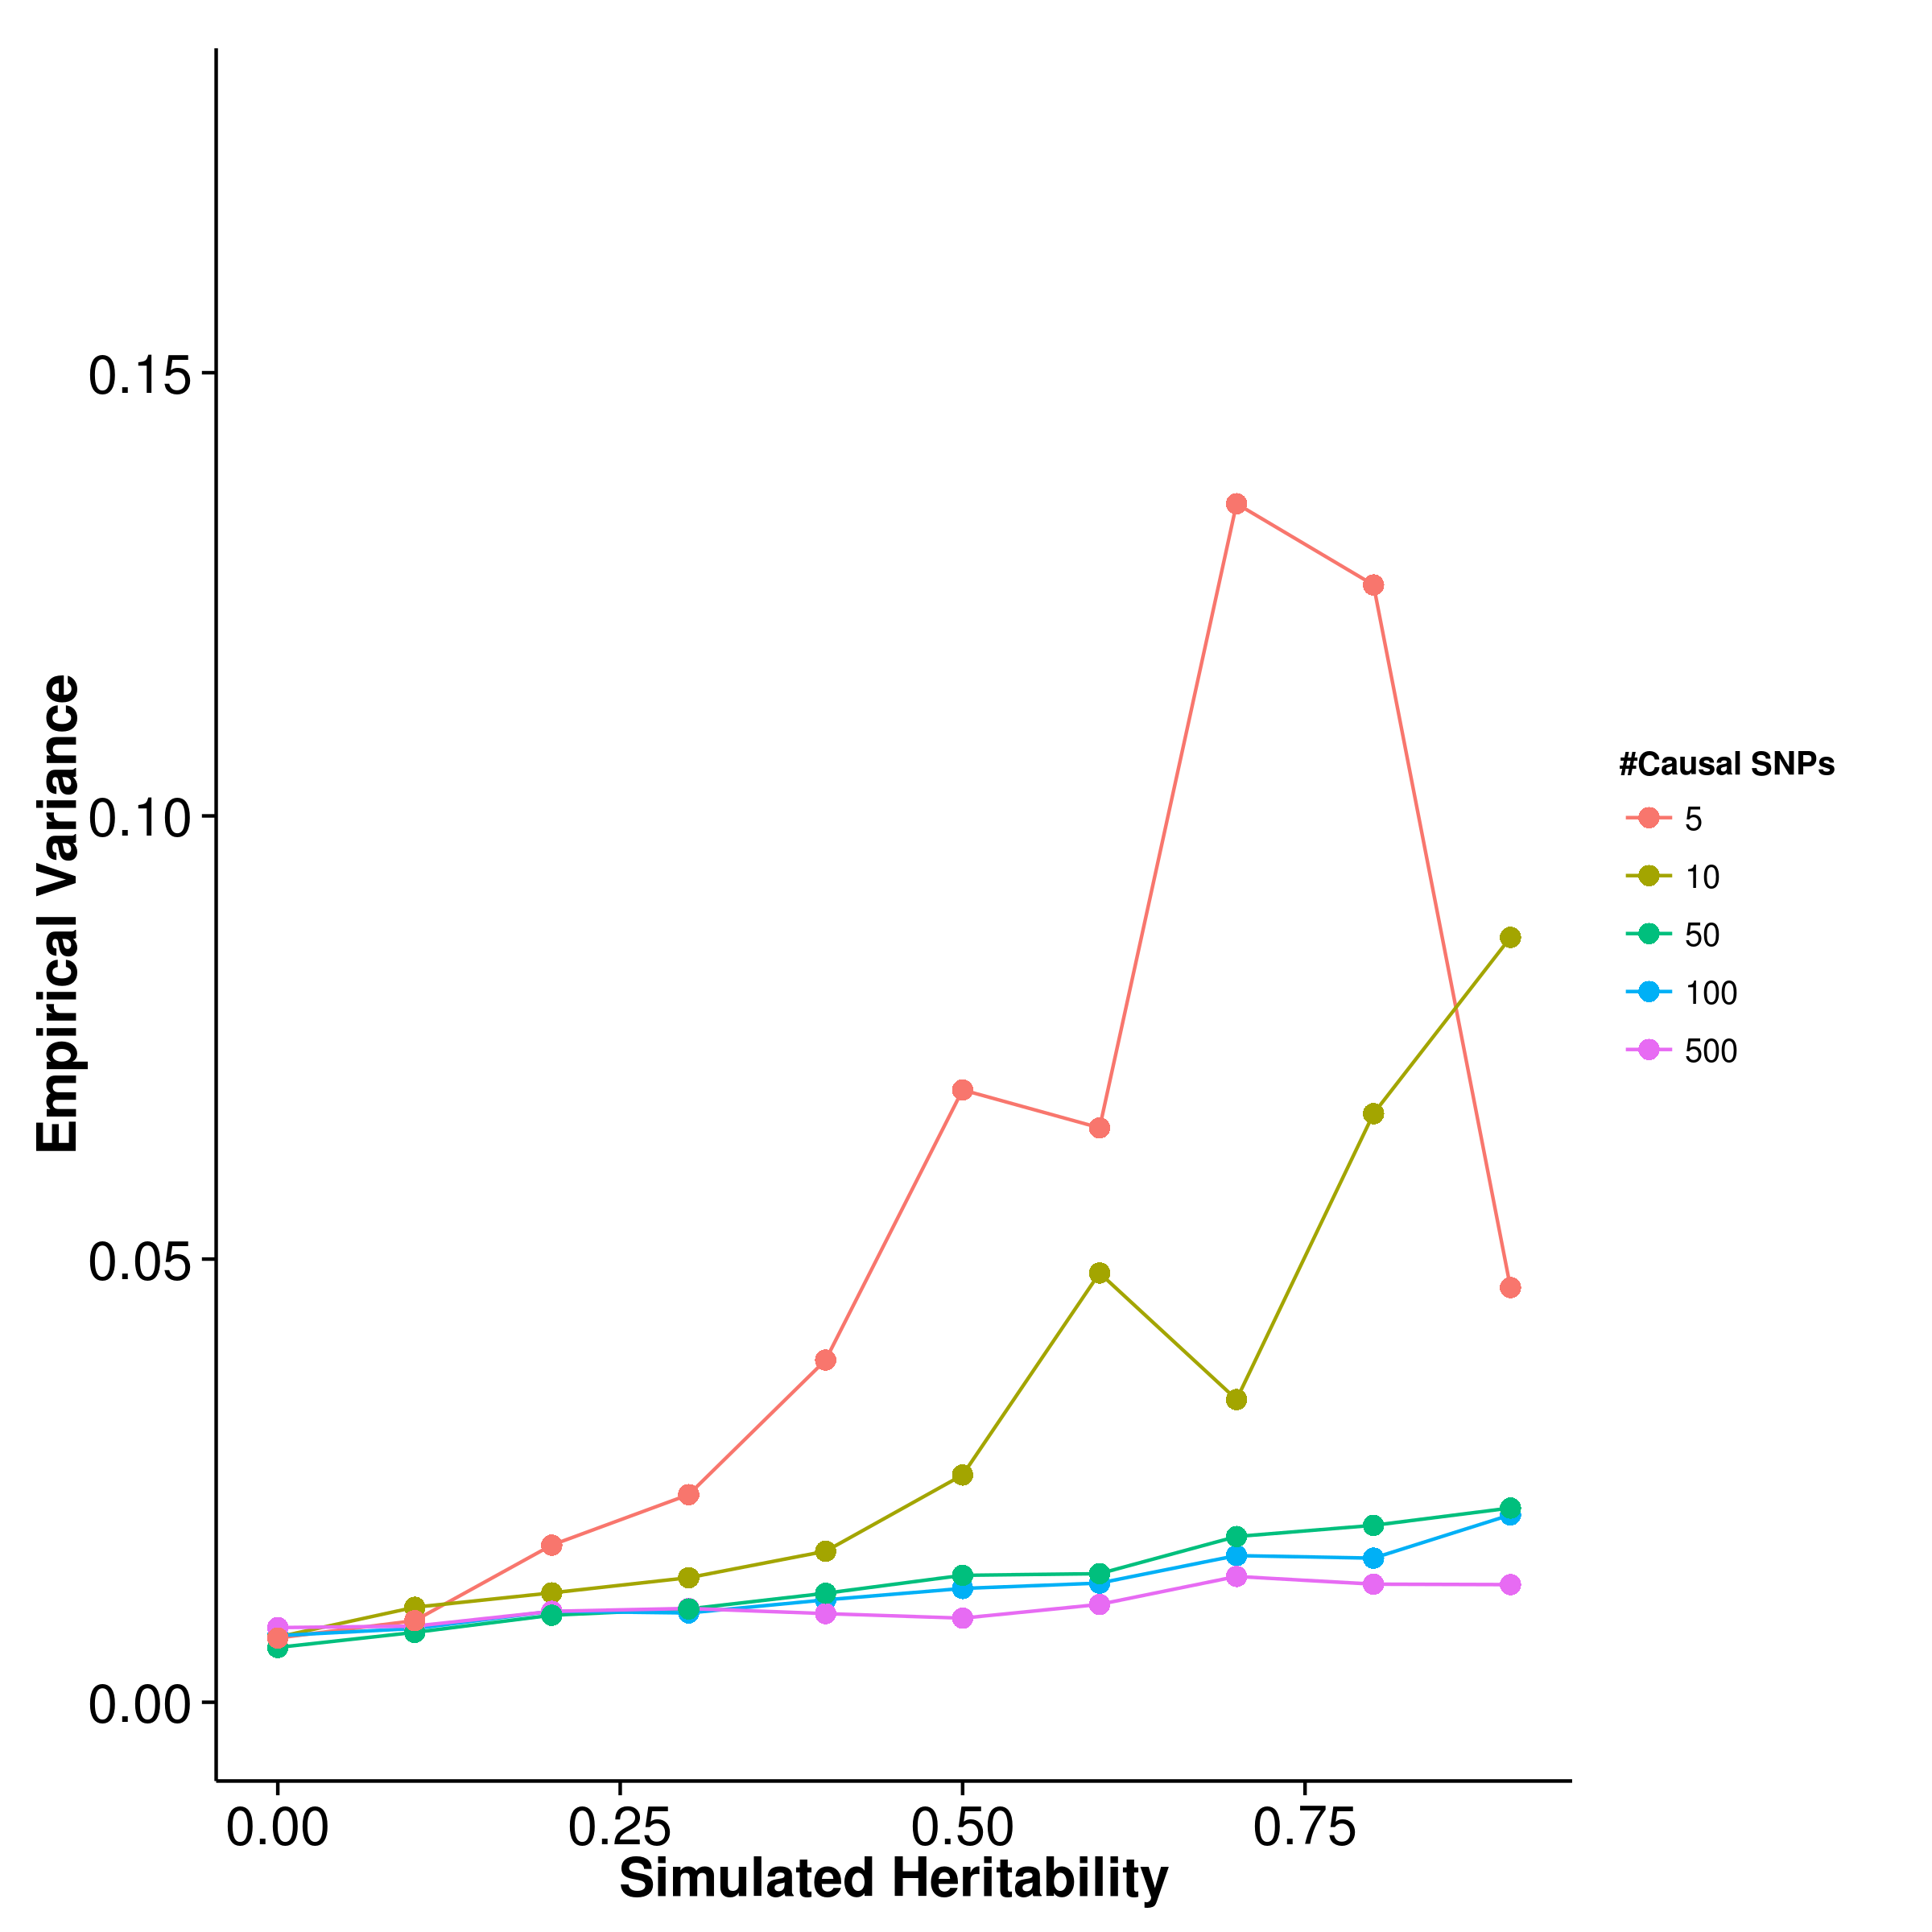
\includegraphics{figure/he_summary/random/ldsc_Qt_Rand_sd.png}}
				\label{fig:ldscQtRandVar}
			}
			\subfloat[LDSC with intercept estimation]{
				
				\scalebox{.4}{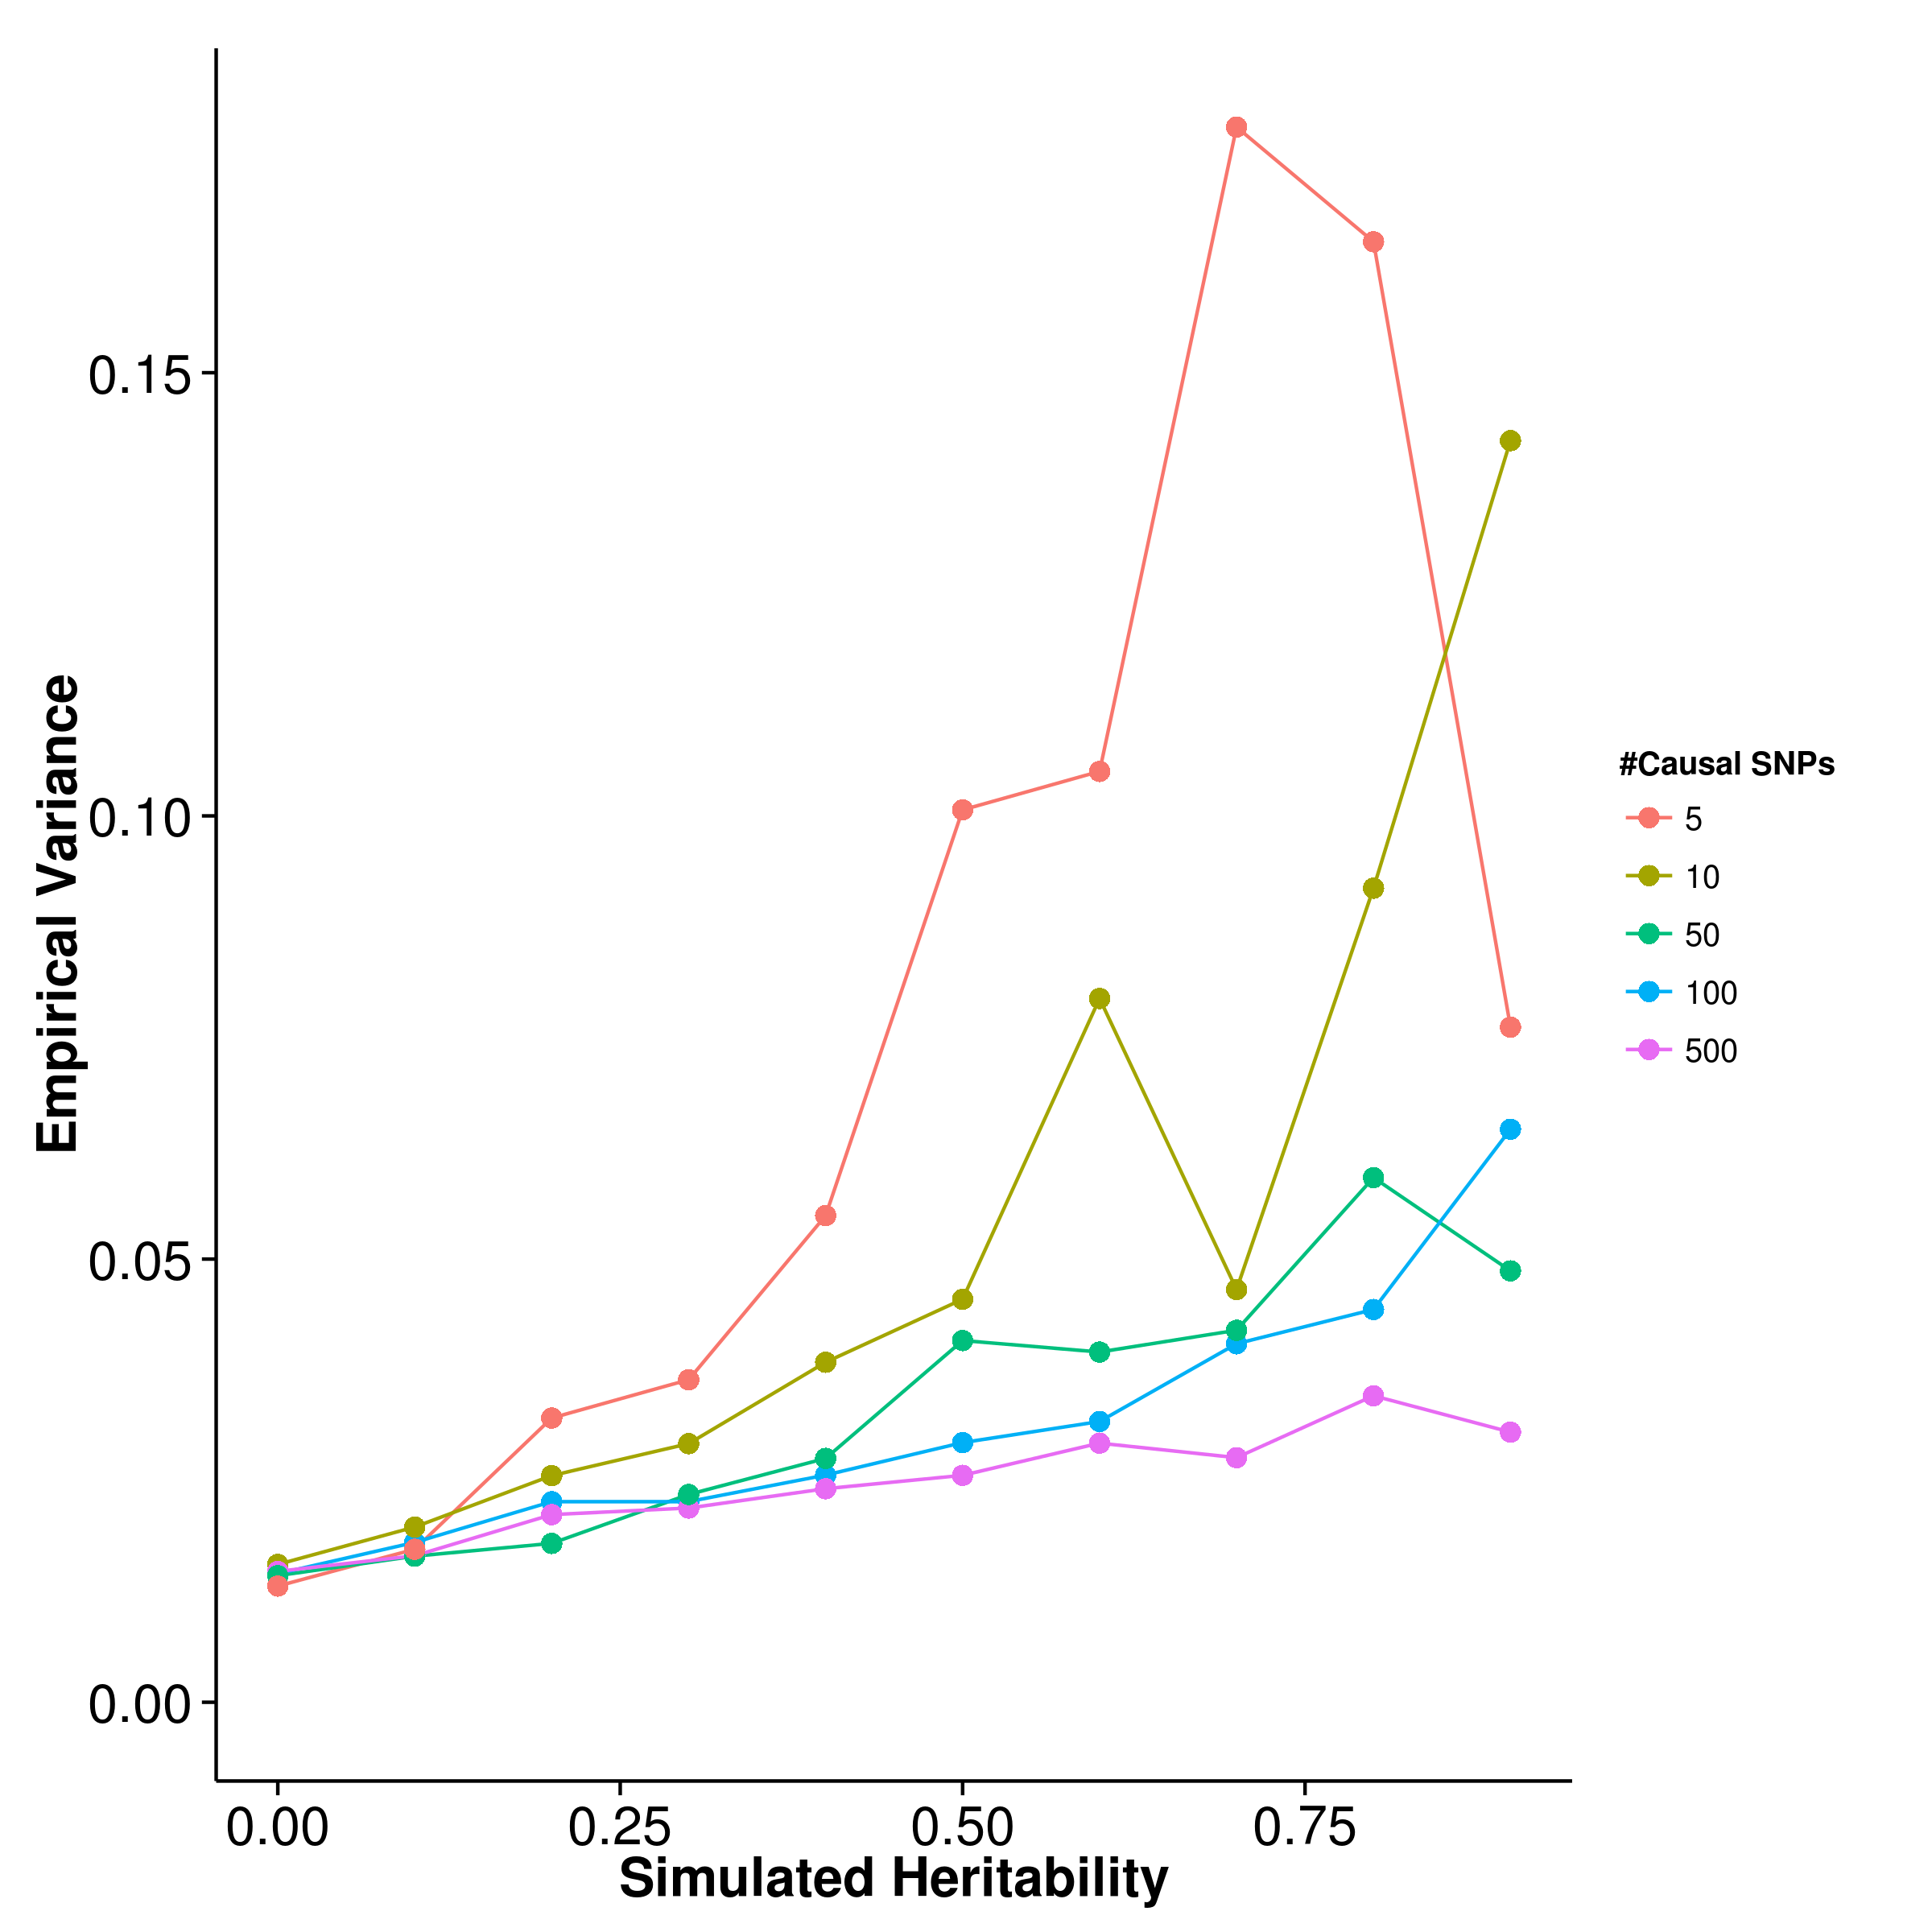
\includegraphics{figure/he_summary/random/ldscIn_Qt_Rand_sd.png}}
				\label{fig:ldscInQtRandVar}
			}
			\caption[Variance of Quantitative Trait Simulation Results]
			{Variance of results from quantitative trait simulation with random effect size simulation.
				Under the polygenic conditions, \gls{gcta} has the smallest variance, follow by \gls{ldsc}. 
				However, it was observed when the number of causal \glspl{SNP} decreases, the variance of the estimation increases for all algorithm, with variance of the \gls{shrek} estimate being the least affected.
				In fact, under oligogenic conditions, \gls{shrek} has a lower empirical variance when compared to \gls{ldsc}.
			} 
			\label{fig:QtRandVar}
		\end{figure}
		
		\begin{figure}
			\centering
			\subfloat[SHREK]{
				\scalebox{.4}{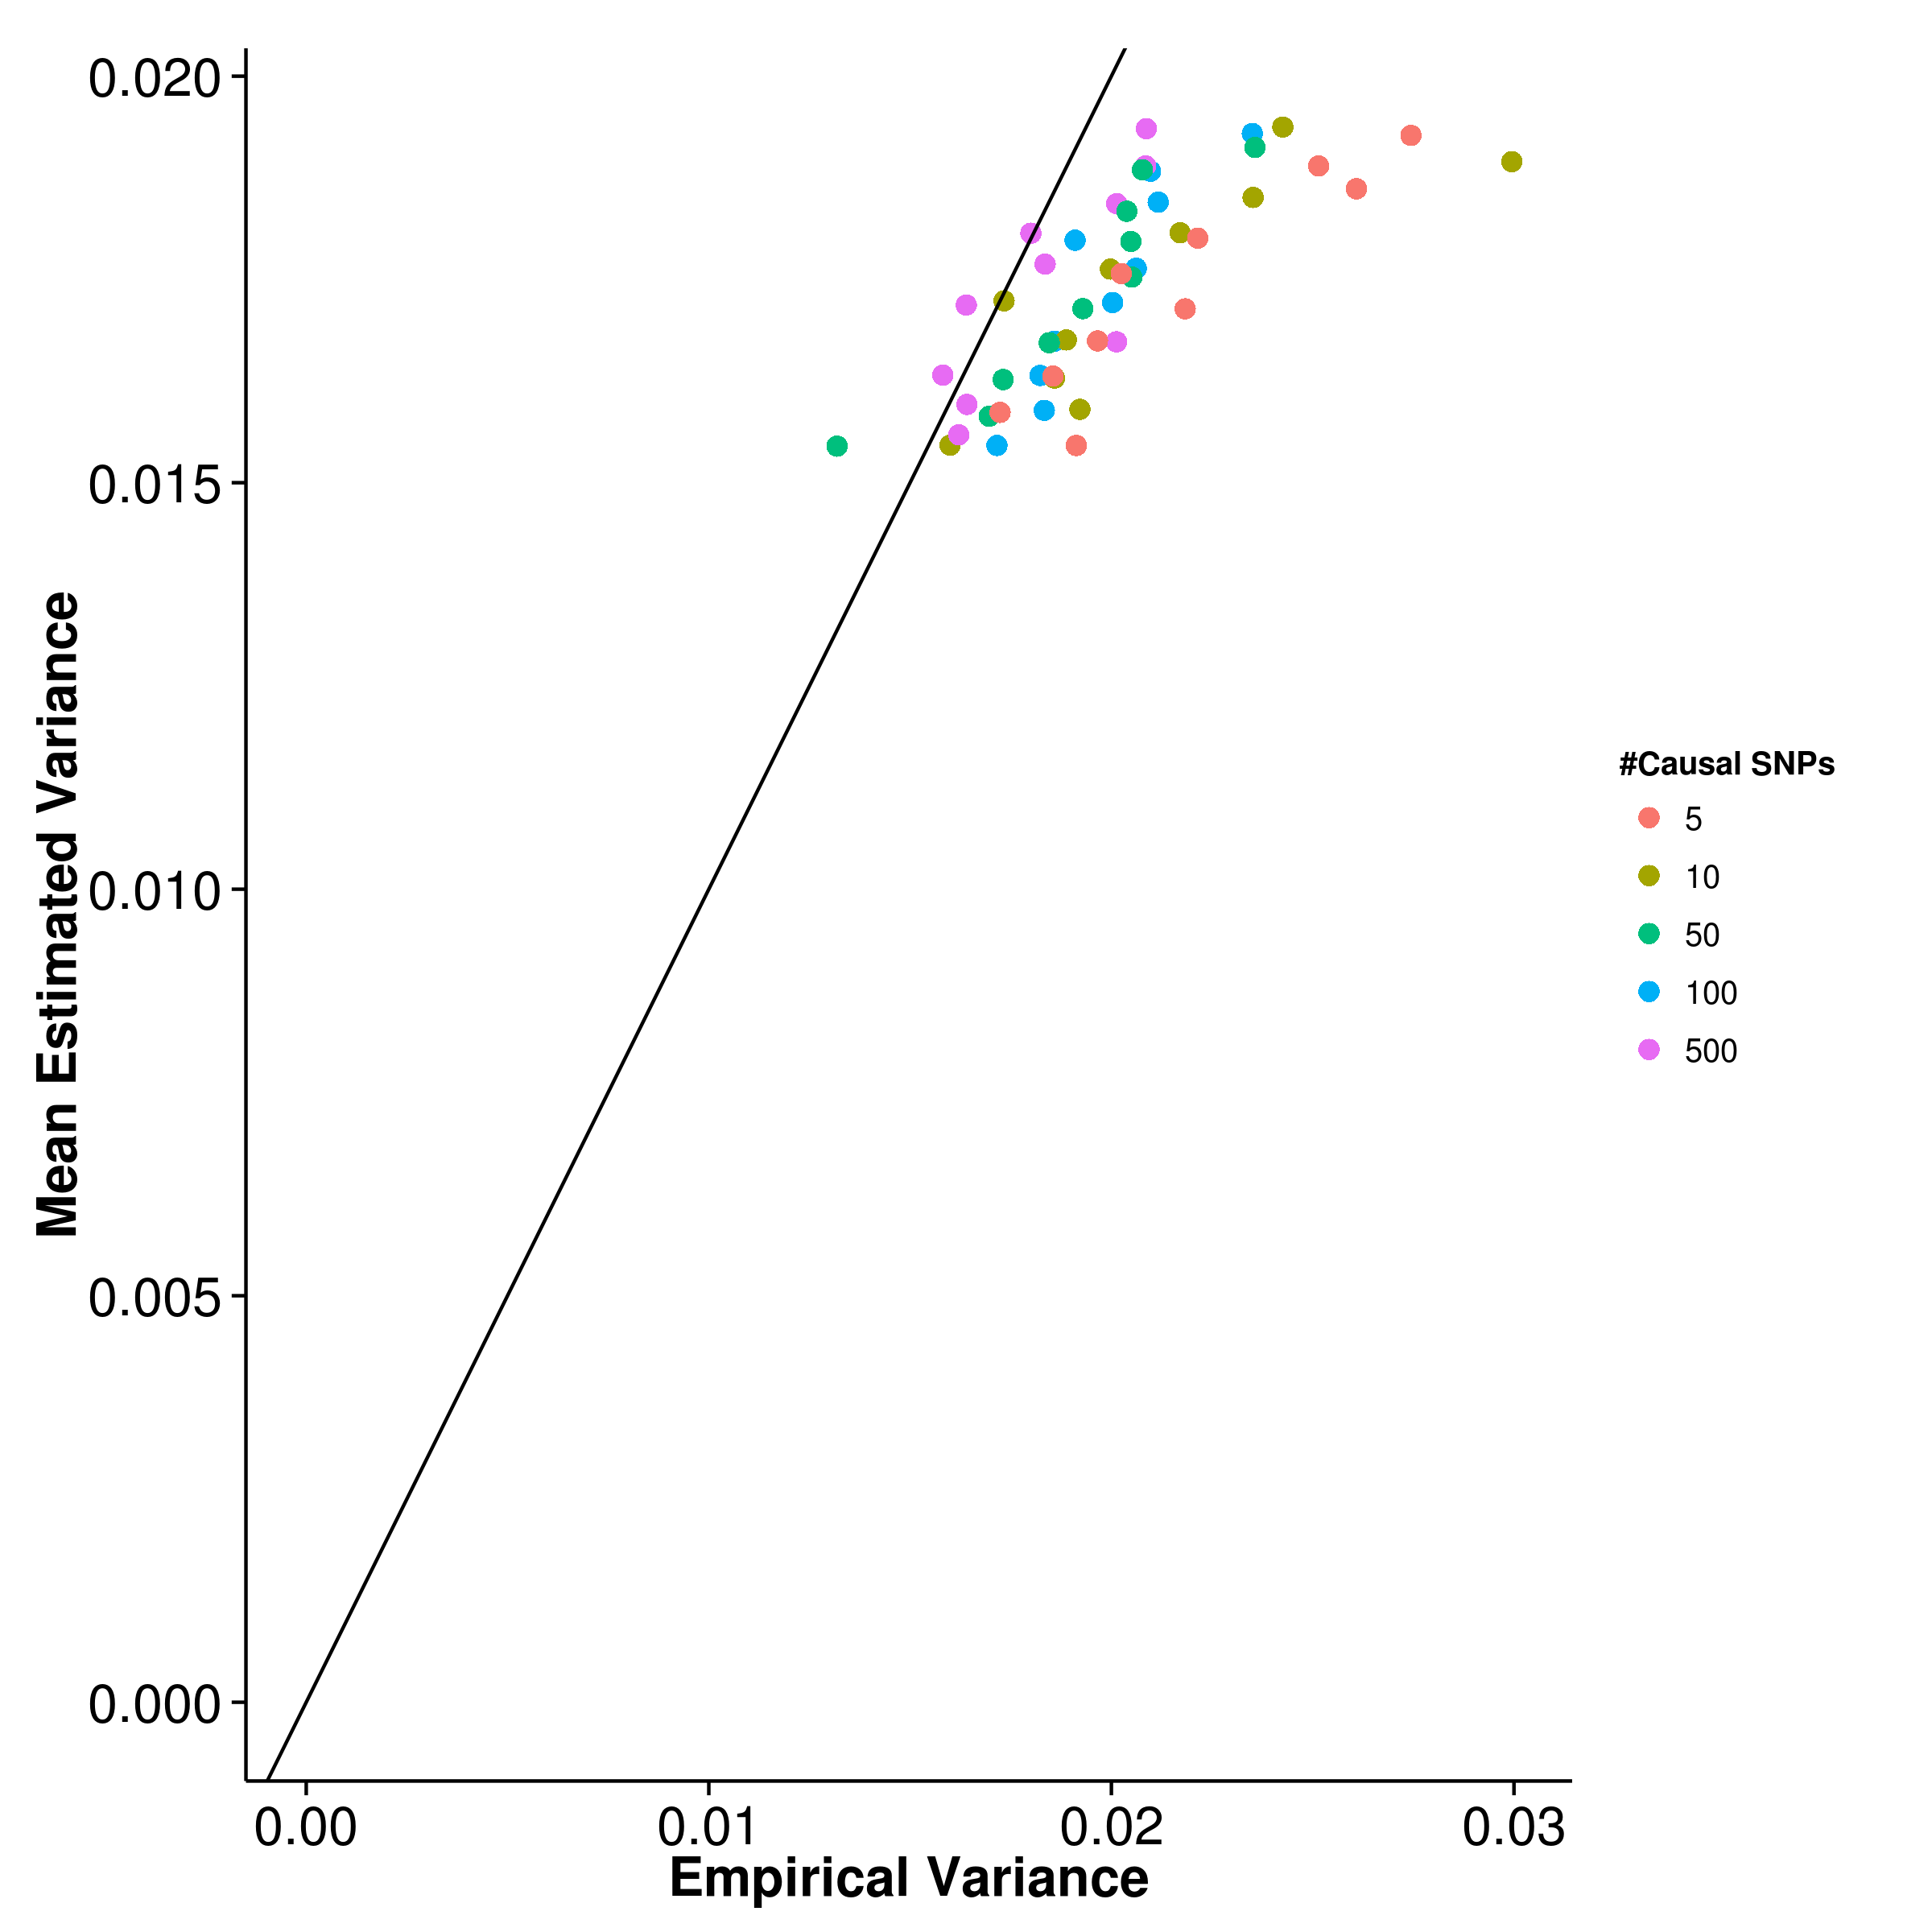
\includegraphics{figure/he_summary/random/shrek_Qt_Rand_sdCom.png}}
				\label{fig:shrekQtRandVarCom}
			}
			\subfloat[GCTA]{
				\scalebox{.4}{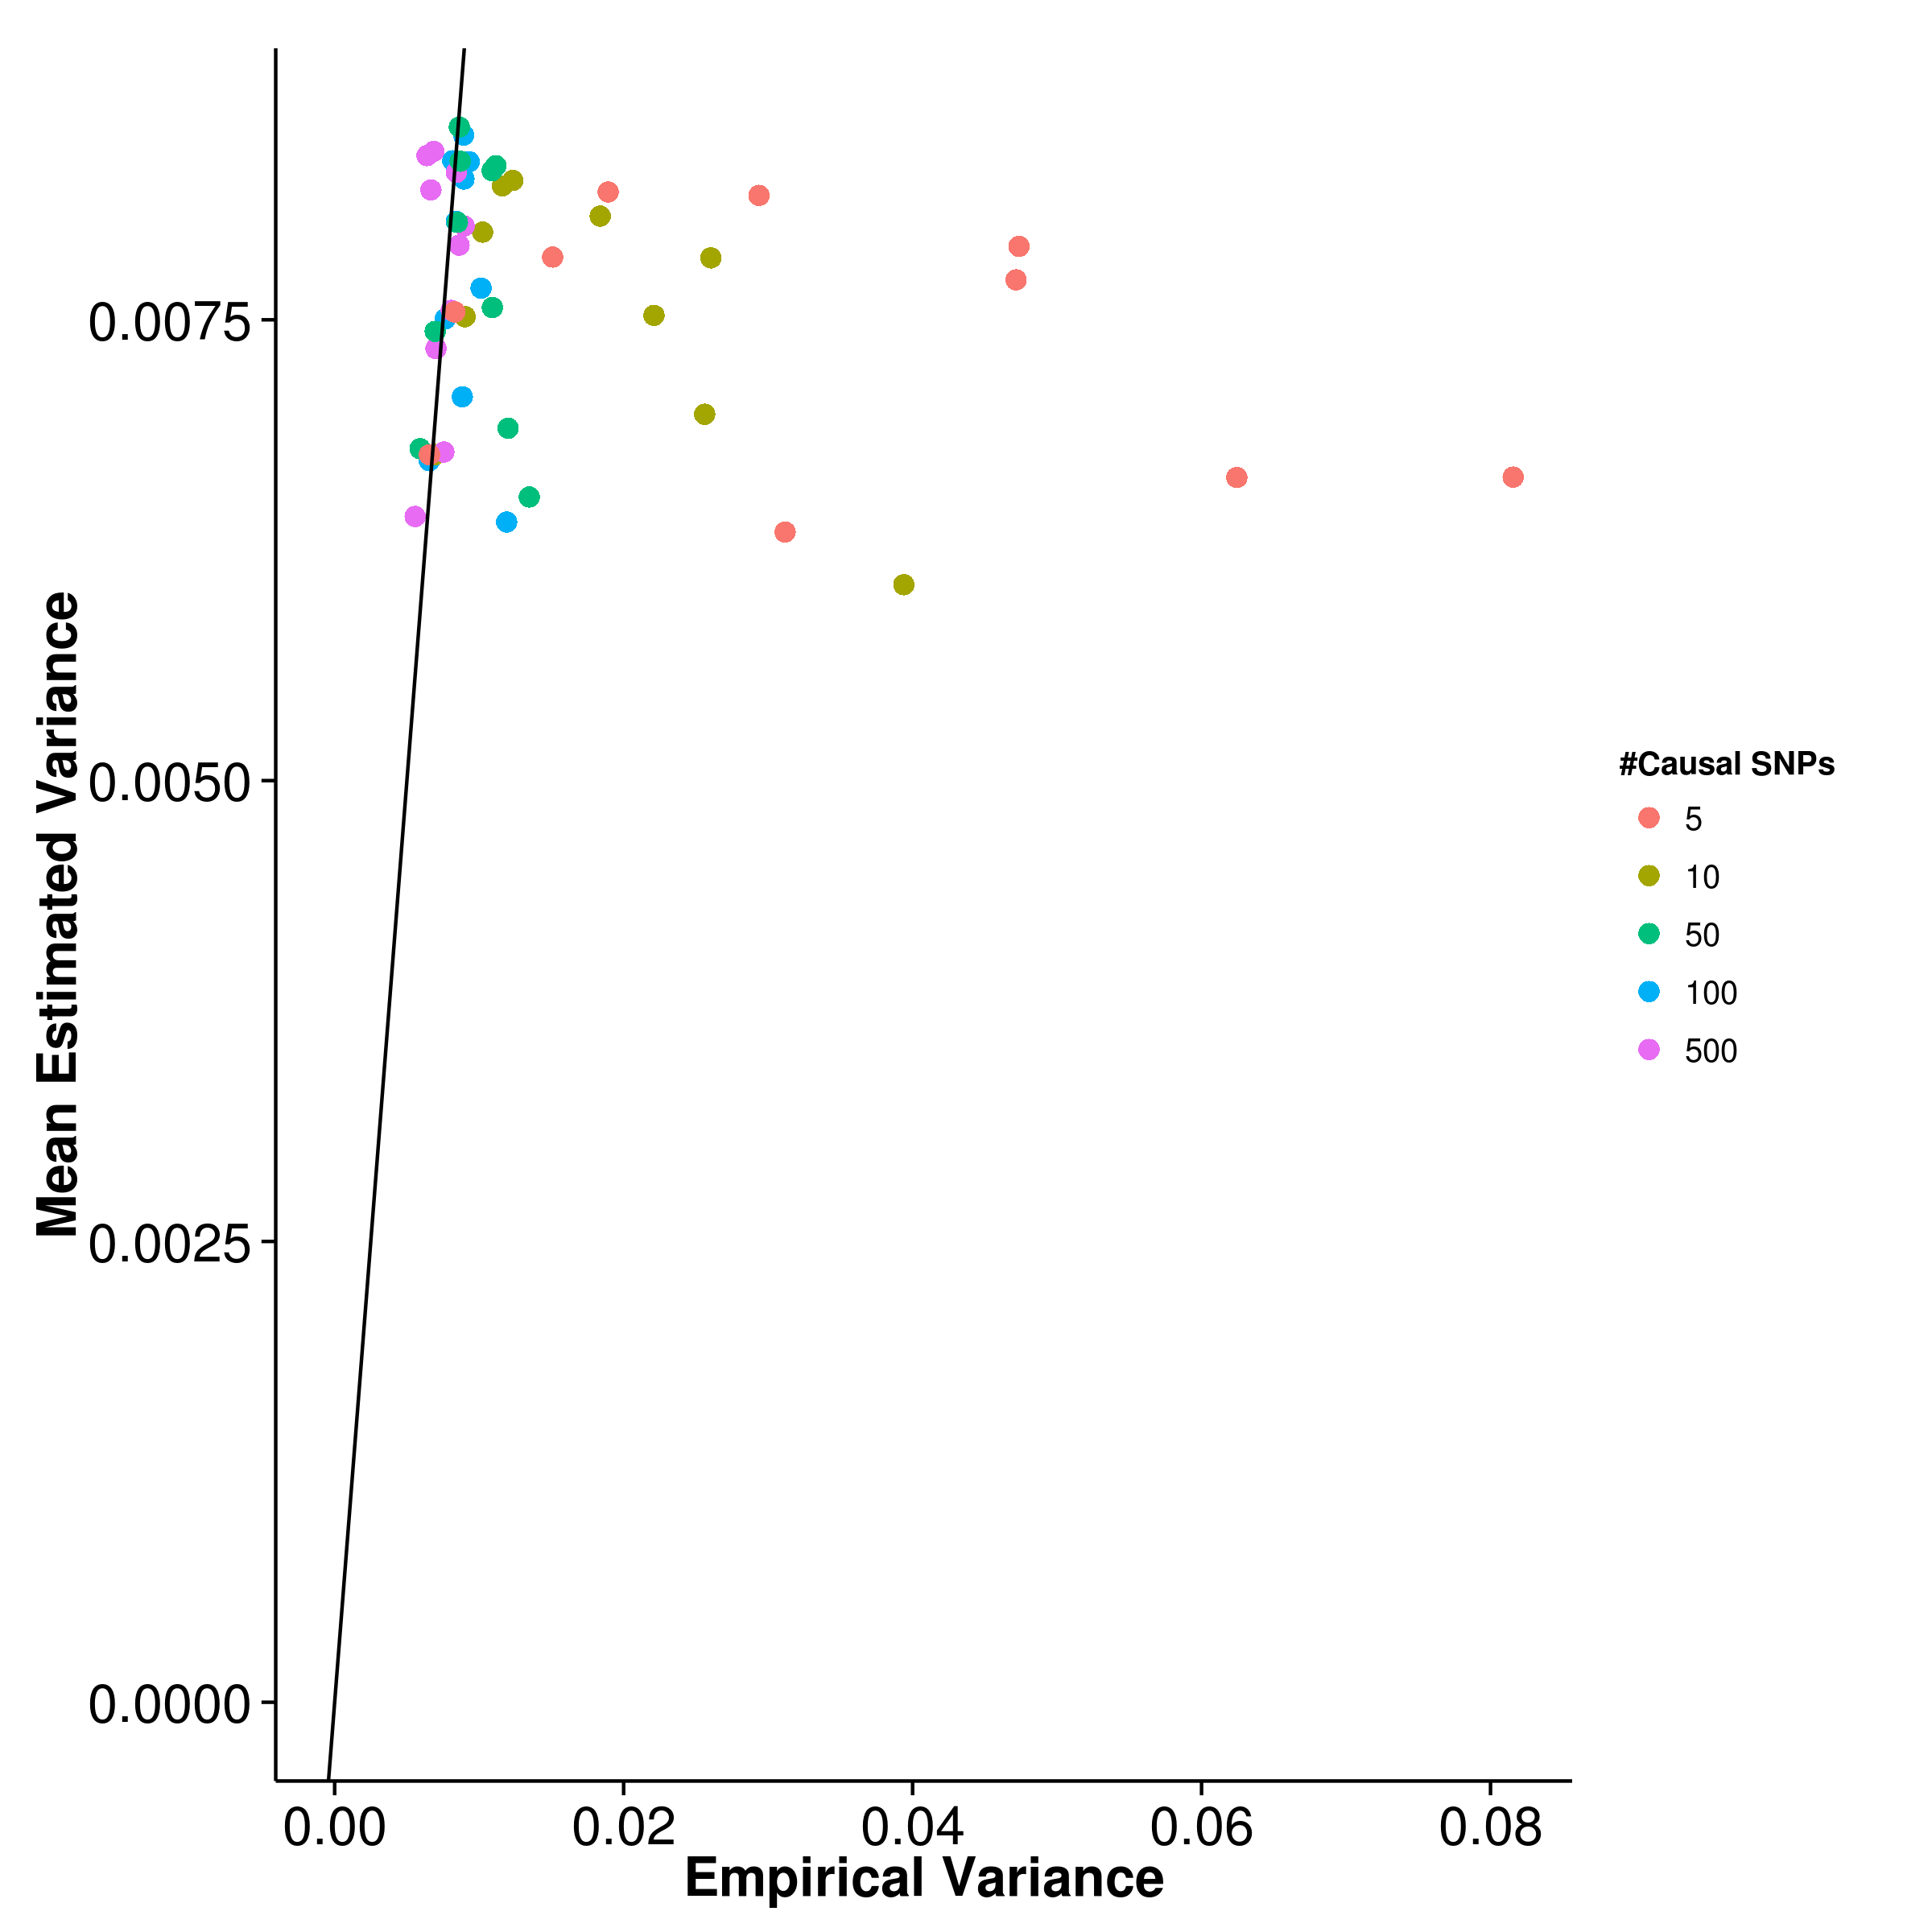
\includegraphics{figure/he_summary/random/gcta_Qt_Rand_sdCom.png}}
				\label{fig:gctaQtRandVarCom}
			}\\
			\subfloat[LDSC with fix intercept]{
				\scalebox{.4}{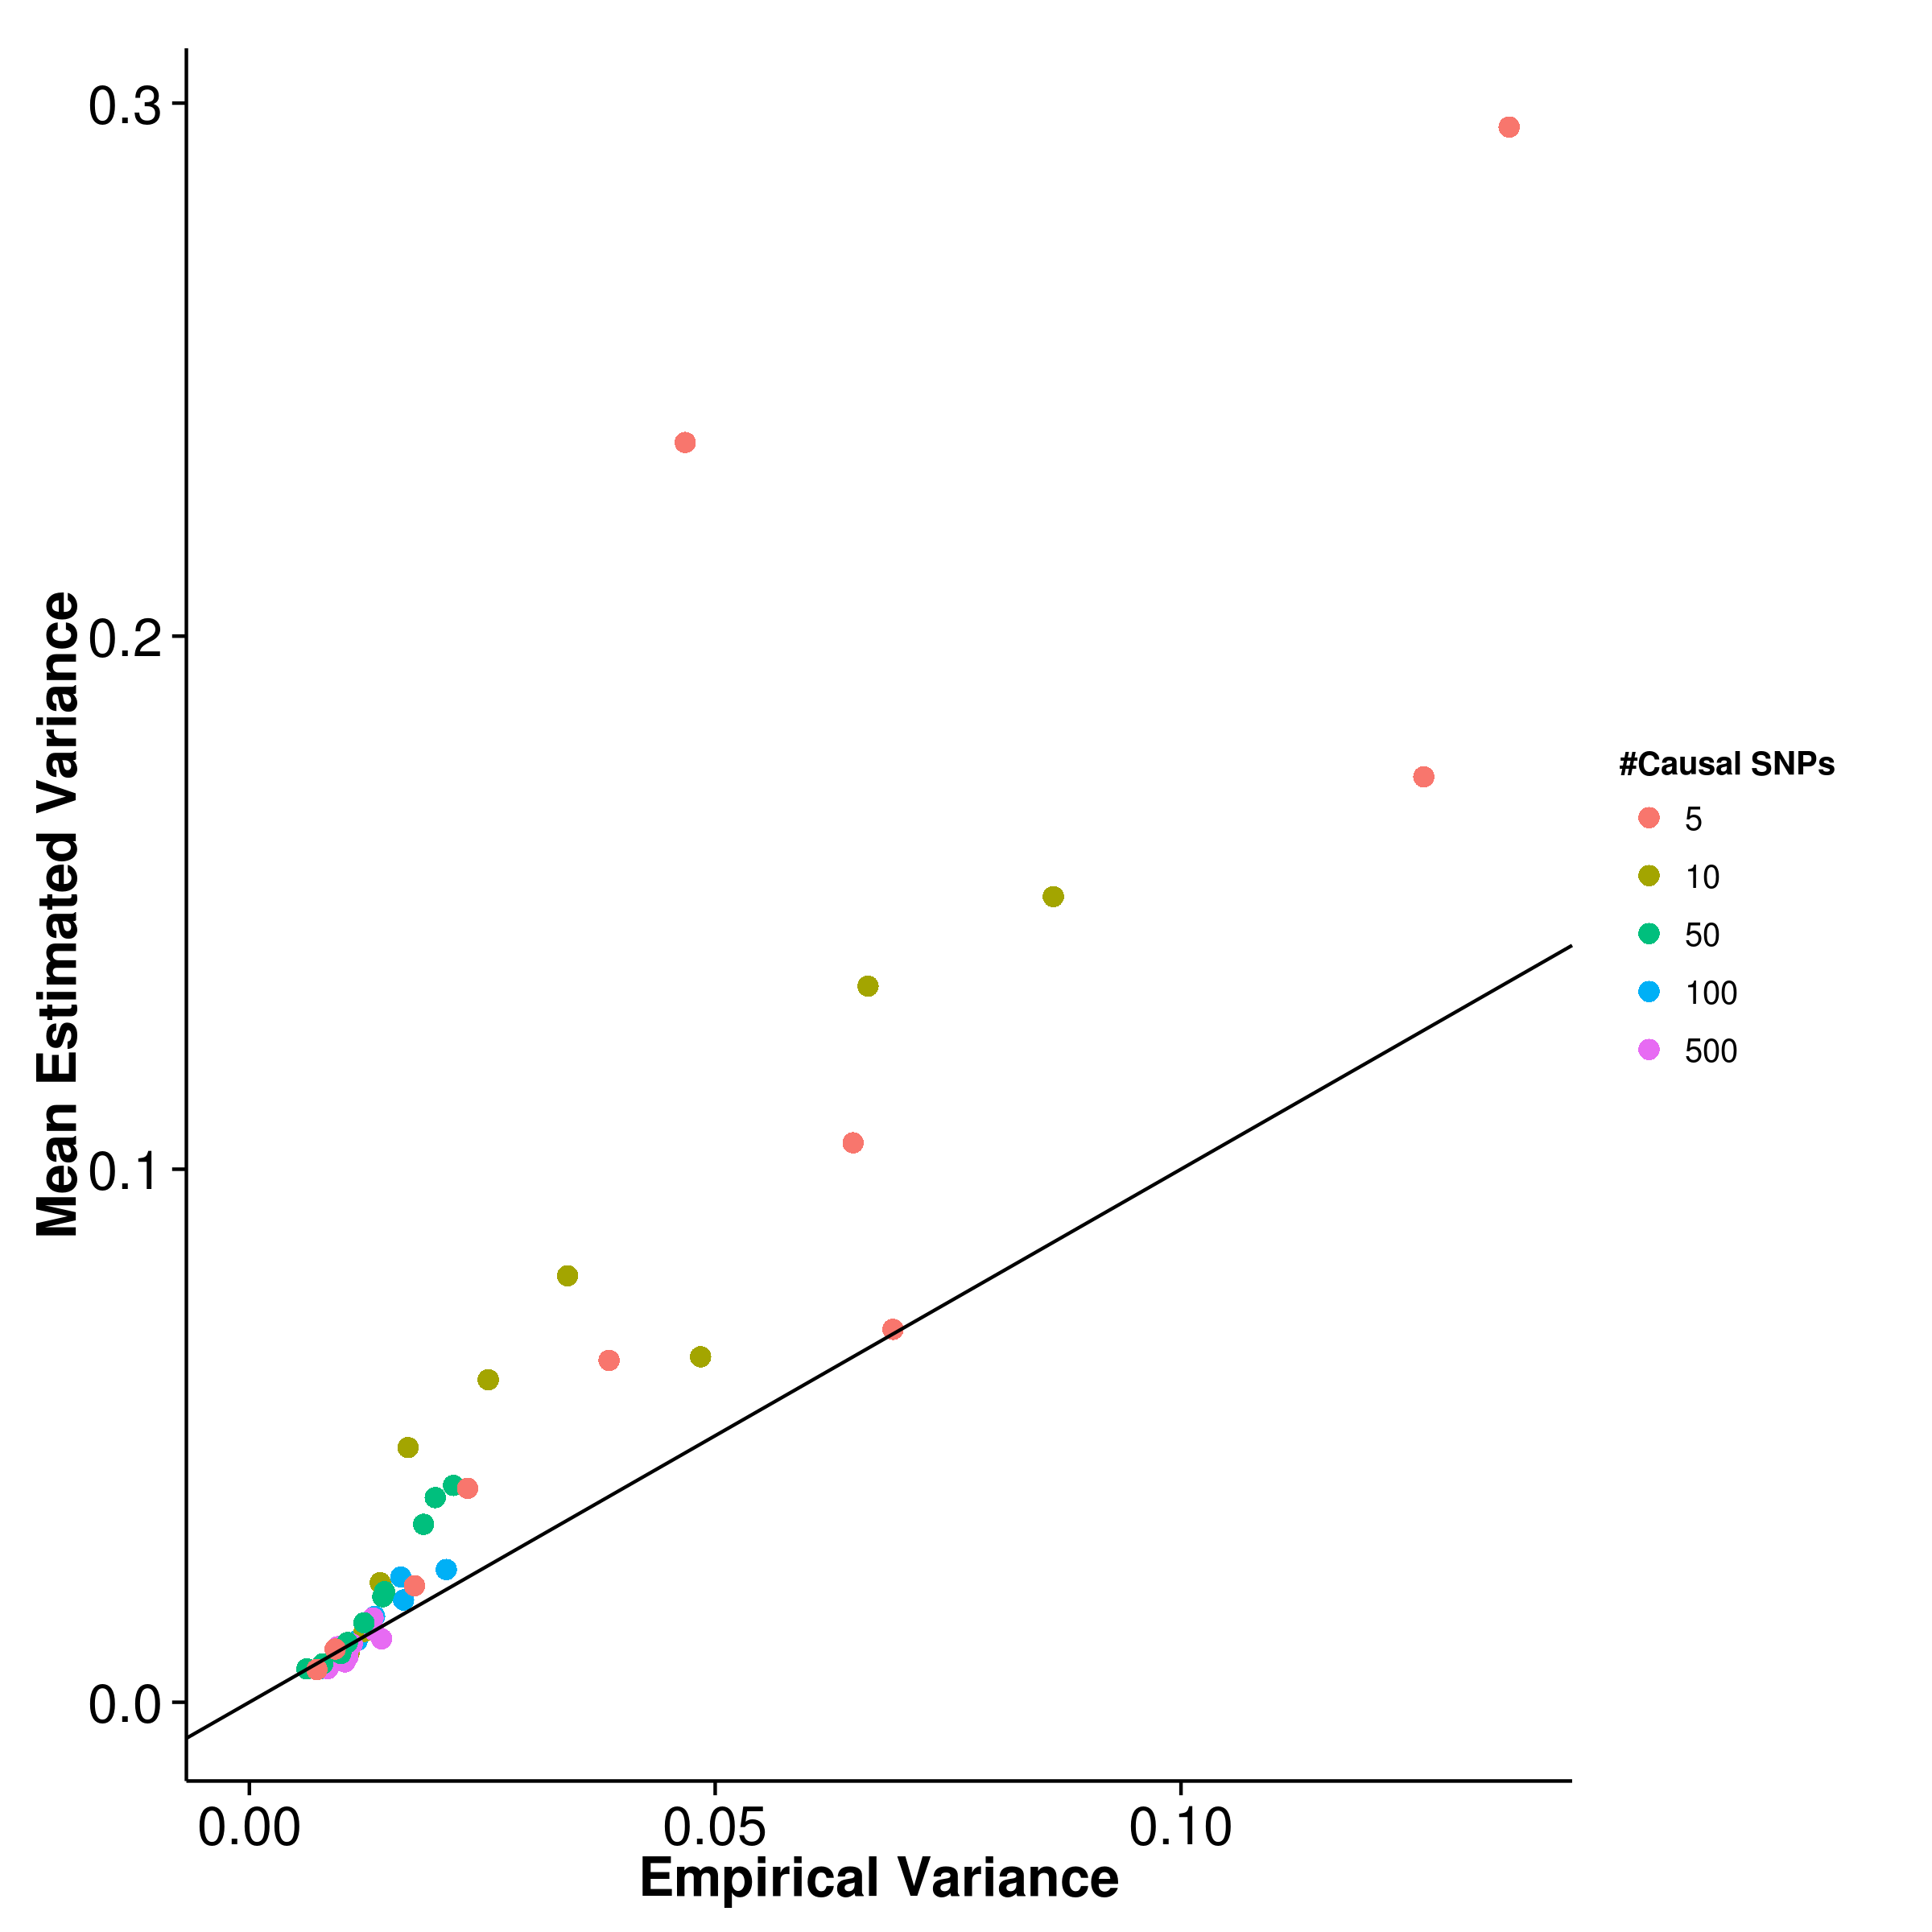
\includegraphics{figure/he_summary/random/ldsc_Qt_Rand_sdCom.png}}
				\label{fig:ldscQtRandVarCom}
			}
			\subfloat[LDSC with intercept estimation]{
				
				\scalebox{.4}{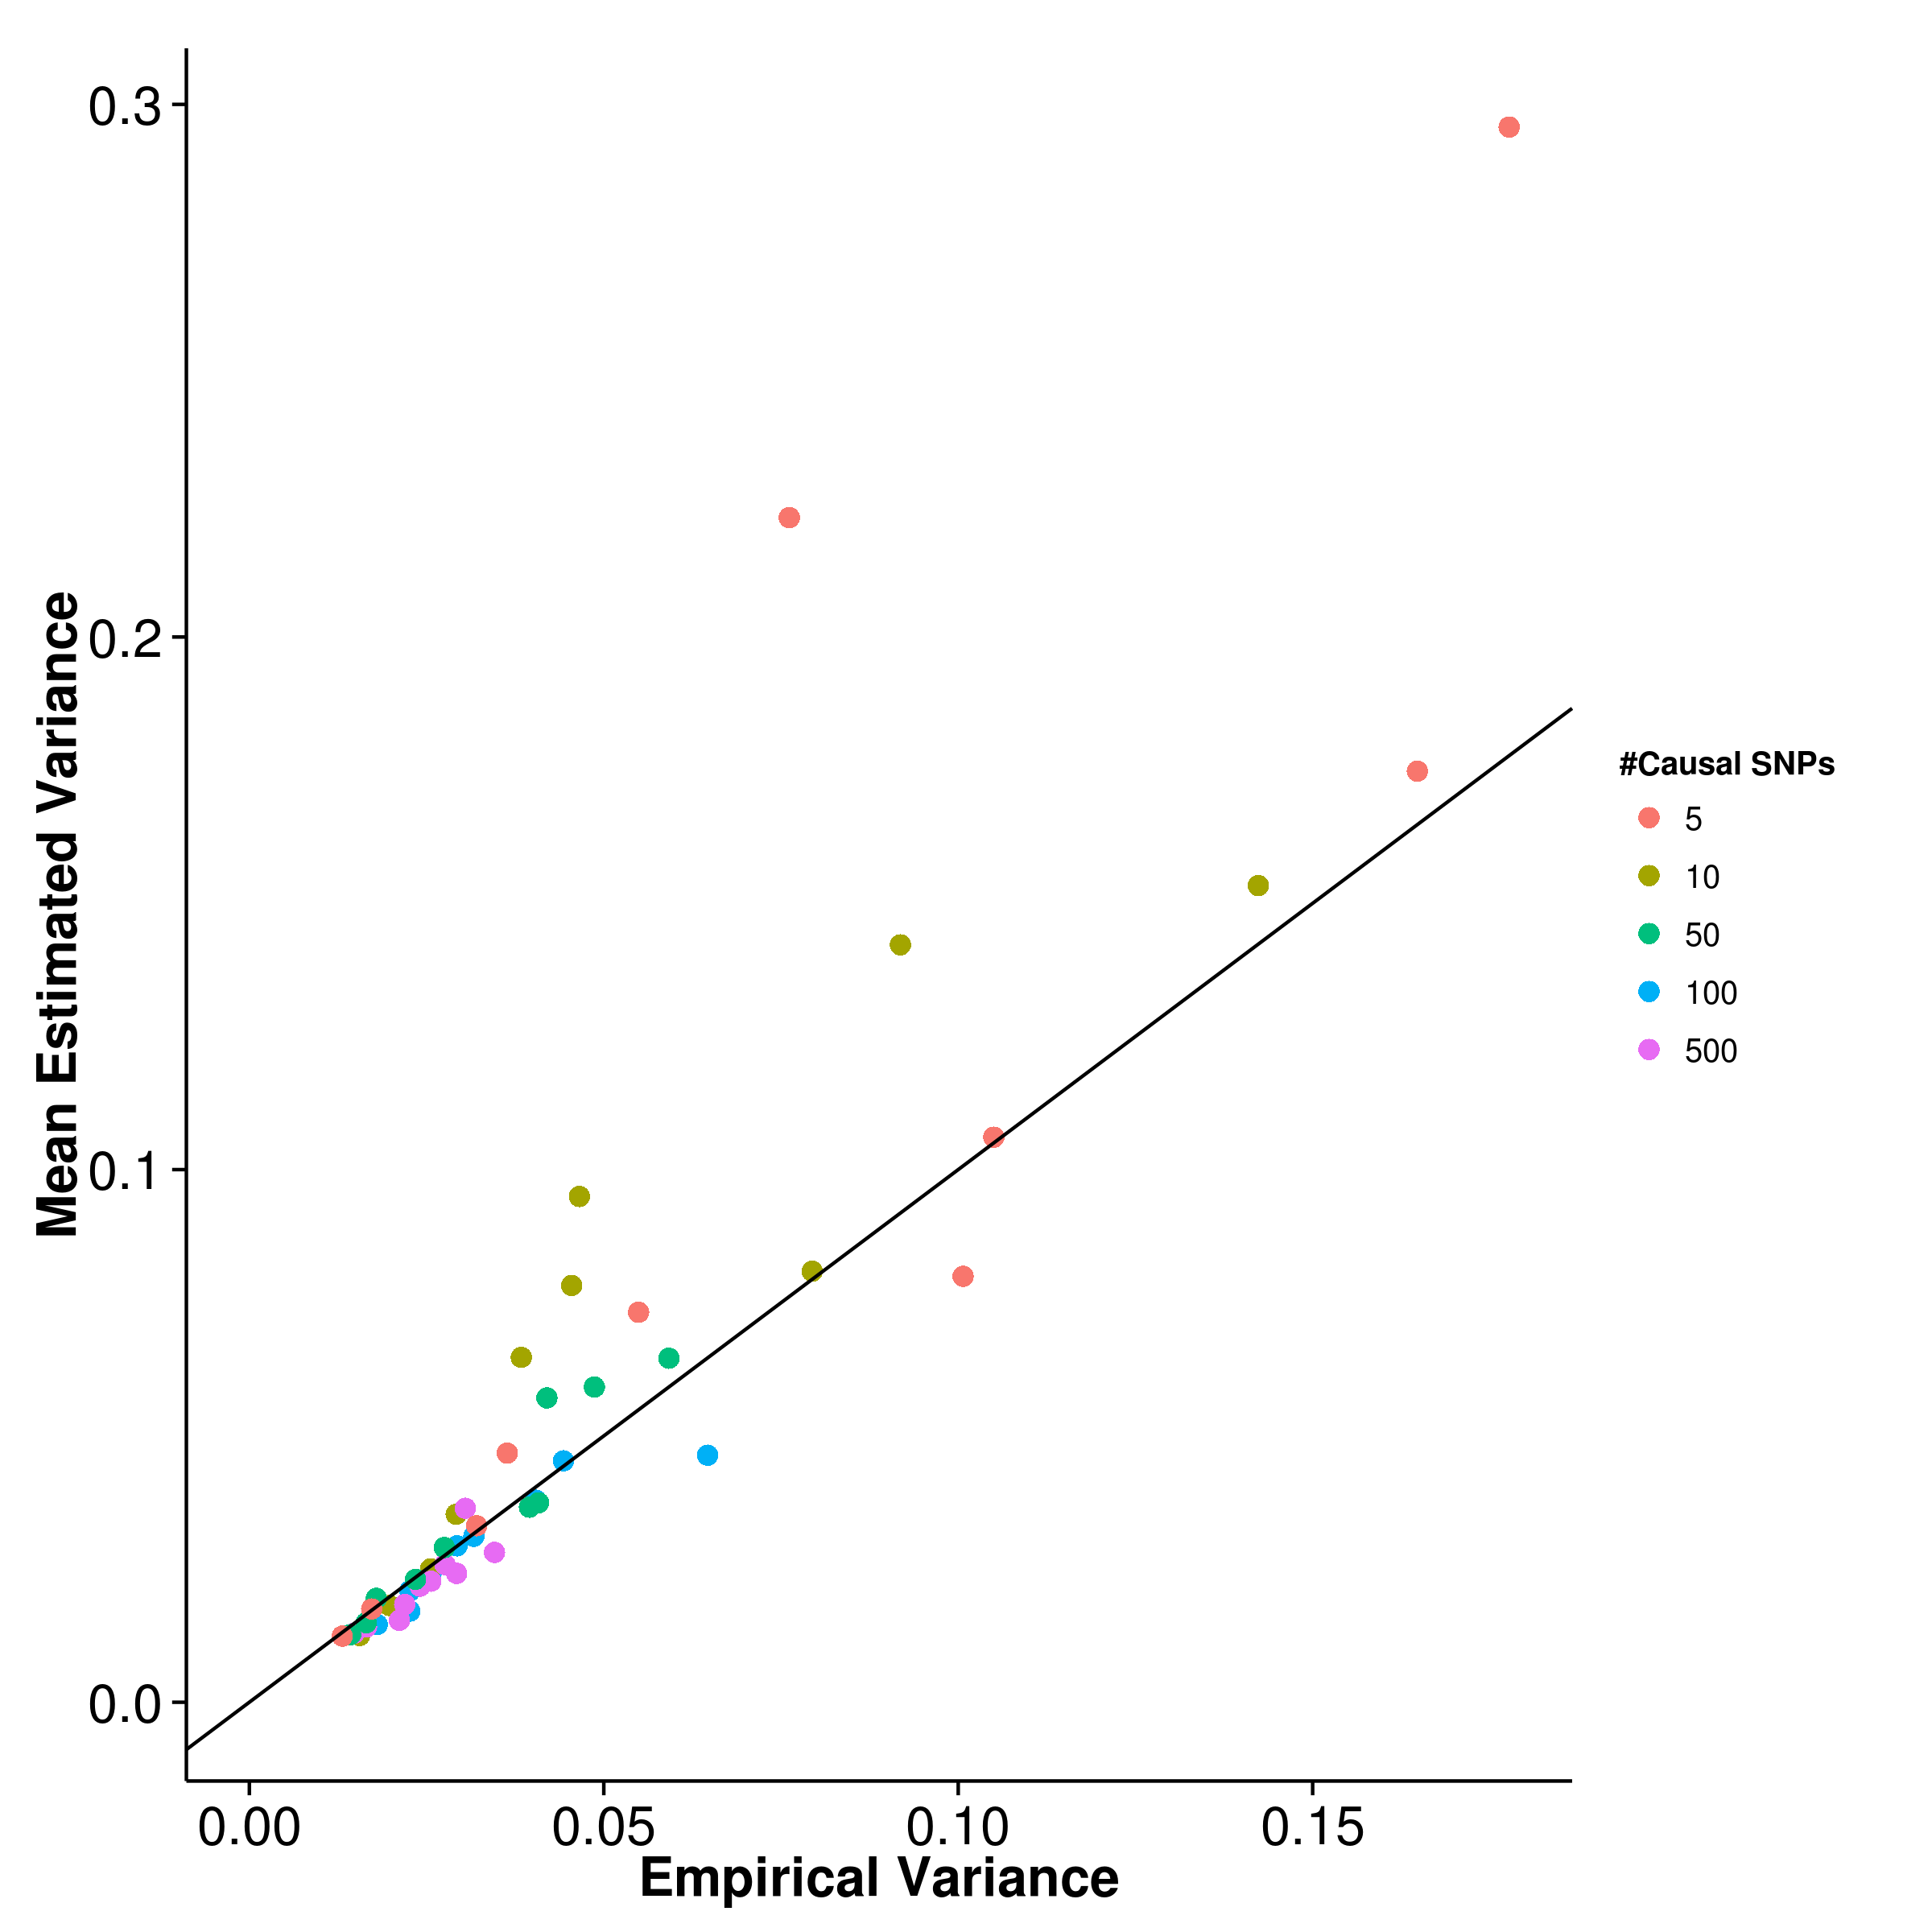
\includegraphics{figure/he_summary/random/ldscIn_Qt_Rand_sdCom.png}}
				\label{fig:ldscInQtRandVarCom}
			}
			\caption[Estimation of Variance in Quantitative Trait Simulation]
			{Estimated variance of results from quantitative trait simulation with random effect size simulation when compared to the empirical variance.
			\gls{gcta} has the best estimate of its empirical variance under the polygenic conditions whereas \gls{shrek} tends to under-estimate its empirical variance.
			On the other hand, \gls{ldsc} to over-estimate the variance especially when the number of causal \glspl{SNP} is small.
				} 
			\label{fig:QtRandVarCom}
		\end{figure} 
		In the simulation of quantitative trait scenario, the effect size were randomly drawn from the exponential distribution with $\lambda=1$ and traits with different number of causal \glspl{SNP} and different narrow sense heritability were simulated.
		The main aim of this simulation was to assess the effect of number of causal \glspl{SNP} and trait heritability on the power of estimation of different algorithms.
		
		First, the mean heritability estimation were compared to the simulated heritability in order to identify the bias in estimation for each algorithms.
		From the graph (\cref{fig:QtRandMean}), it was observed that the mean estimations of \gls{shrek} has a small upward bias (\cref{fig:shrekQtRandMean}).
		However, the bias was insensitive to the change in number of causal \glspl{SNP} suggesting that \gls{shrek} is relatively robust to trait complexity.
		On the other hand, estimations form \gls{gcta} were moderately biased downward (\cref{fig:gctaQtRandMean}), similar to the estimations from \gls{ldsc} with intercept estimation (\cref{fig:ldscInQtRandMean}), but with a smaller variability.
		Finally, when the intercept is fixed, \gls{ldsc} has the smallest bias when the trait is polygenic but an upward bias is also observed when the number of causal \glspl{SNP} is small.
		
		
		Furthermore, while comparing the empirical variance of the estimates (\cref{fig:QtRandVar}), variance of estimations from \gls{ldsc} were sensitive to the number of causal \glspl{SNP} where as the number of causal \glspl{SNP} decreases (\cref{fig:ldscQtRandVar,fig:ldscInQtRandVar}), the variance increases, similar to what was reported by \citet{Bulik-Sullivan2015}.
		The variance were also higher when intercept estimation was performed. 
		On the other hand, although the variance of \gls{shrek} was relatively higher when compared to \gls{ldsc} when the intercept was fixed, the variation of its estimations was insensitive to the number of causal \glspl{SNP}, when the number of causal \glspl{SNP} was small, the variance of estimation from \gls{shrek} can be even be lower than \gls{ldsc} (\cref{fig:shrekQtRandVar}).
		Finally, of all the algorithms, the estimations from \gls{gcta} has the lowest variation when compared to other algorithm (\cref{fig:gctaQtRandVar}), except when it was the case of 5 causal \glspl{SNP} where it has a slightly higher variance when compared to \gls{shrek} when the simulated heritability was high (e.g. $\ge 0.8$).
		

		Another important factor to consider was the estimation of the \gls{se}. 
		Of all the algorithms, \gls{gcta} (\cref{fig:gctaQtRandVarCom}) has the best estimate, follow by \gls{shrek} (\cref{fig:shrekQtRandVarCom}).
		However, it was noted that a consistent underestimation of variance was observed with \gls{shrek} whereas \gls{gcta} only underestimate the variance when the number of causal \glspl{SNP} is small.
		On the other hand, when the intercept was fixed (\cref{fig:ldscQtRandVarCom}), \gls{ldsc} cannot accurately estimate its variance and tends to overestimate, especially when the number of causal \glspl{SNP} were small. 
		When intercept estimations was performed (\cref{fig:ldscInQtRandVarCom}), the estimation of variance was relatively better yet the overestimation were still observed when the number of causal \glspl{SNP} is small. 
		
		By taking into consideration of both the bias and variance of the estimates, \gls{gcta} has the best overall performance. 
		Under the oligogenic condition (e.g. number of causal \glspl{SNP} $\le10$), \gls{shrek} has relatively better performance when compared to \gls{ldsc}.
		Whereas under the polygogenic condition, \gls{ldsc} has better performance. 
		%An interesting feature of \gls{shrek} is its relatively robustness towards different genetic structure where the change in number of causal \glspl{SNP} has minimum impact to its performance. 
		%If one is uncertain whether if their trait is polygenic, \gls{shrek} might serves as an alternative to \gls{ldsc}.
		
		\begin{table}
			\centering
			\begin{tabular}{rrrrr}
				\toprule
				Number of Causal SNPs&	SHREK&	LDSC&	LDSC-In&	GCTA \\
				\midrule
				5	&	0.0235	&	0.0576	&	0.0828	&	0.0365\\
				10	&	0.0231	&	0.0343	&	0.0555	&	0.0189\\
				50	&	0.0196	&	0.0157	&	0.0494	&	0.0114\\
				100	&	0.0210	&	0.0129	&	0.0363	&	0.00961\\
				500	&	0.0205	&	0.0115	&	0.0308	&	0.00887\\
				\bottomrule
			\end{tabular}
			\caption[MSE of Quantitative Trait Simulation with Random Effect Size]{
				\Gls{mse} of quantitative trait simulation with random effect size.
				Of all the algorithms, \gls{gcta} has the lowest \gls{mse} except when there is only 5 causal \glspl{SNP}.
				When comparing the performance of \gls{shrek} and \gls{ldsc} with fixed intercept, the performance of \gls{shrek} is better under the oligogenic condition whereas \gls{ldsc} with fixed intercept excels under the polygenic condition. 
				On the other hand, when intercept estimation were performed, the \gls{mse} of \gls{ldsc} increases, mainly due to the increased \gls{se}. 
				Therefore \gls{shrek} out perform \gls{ldsc} with intercept estimation when there are minimal confounding variables.
				}
			\label{tab:mseQtRandom}
		\end{table}
		% Extreme with 100 causal
		
		\subsubsection{Quantitative Trait Simulation with Extreme Effect Size}
		
		\begin{figure}
			\centering
			\subfloat[SHREK]{
				\scalebox{.4}{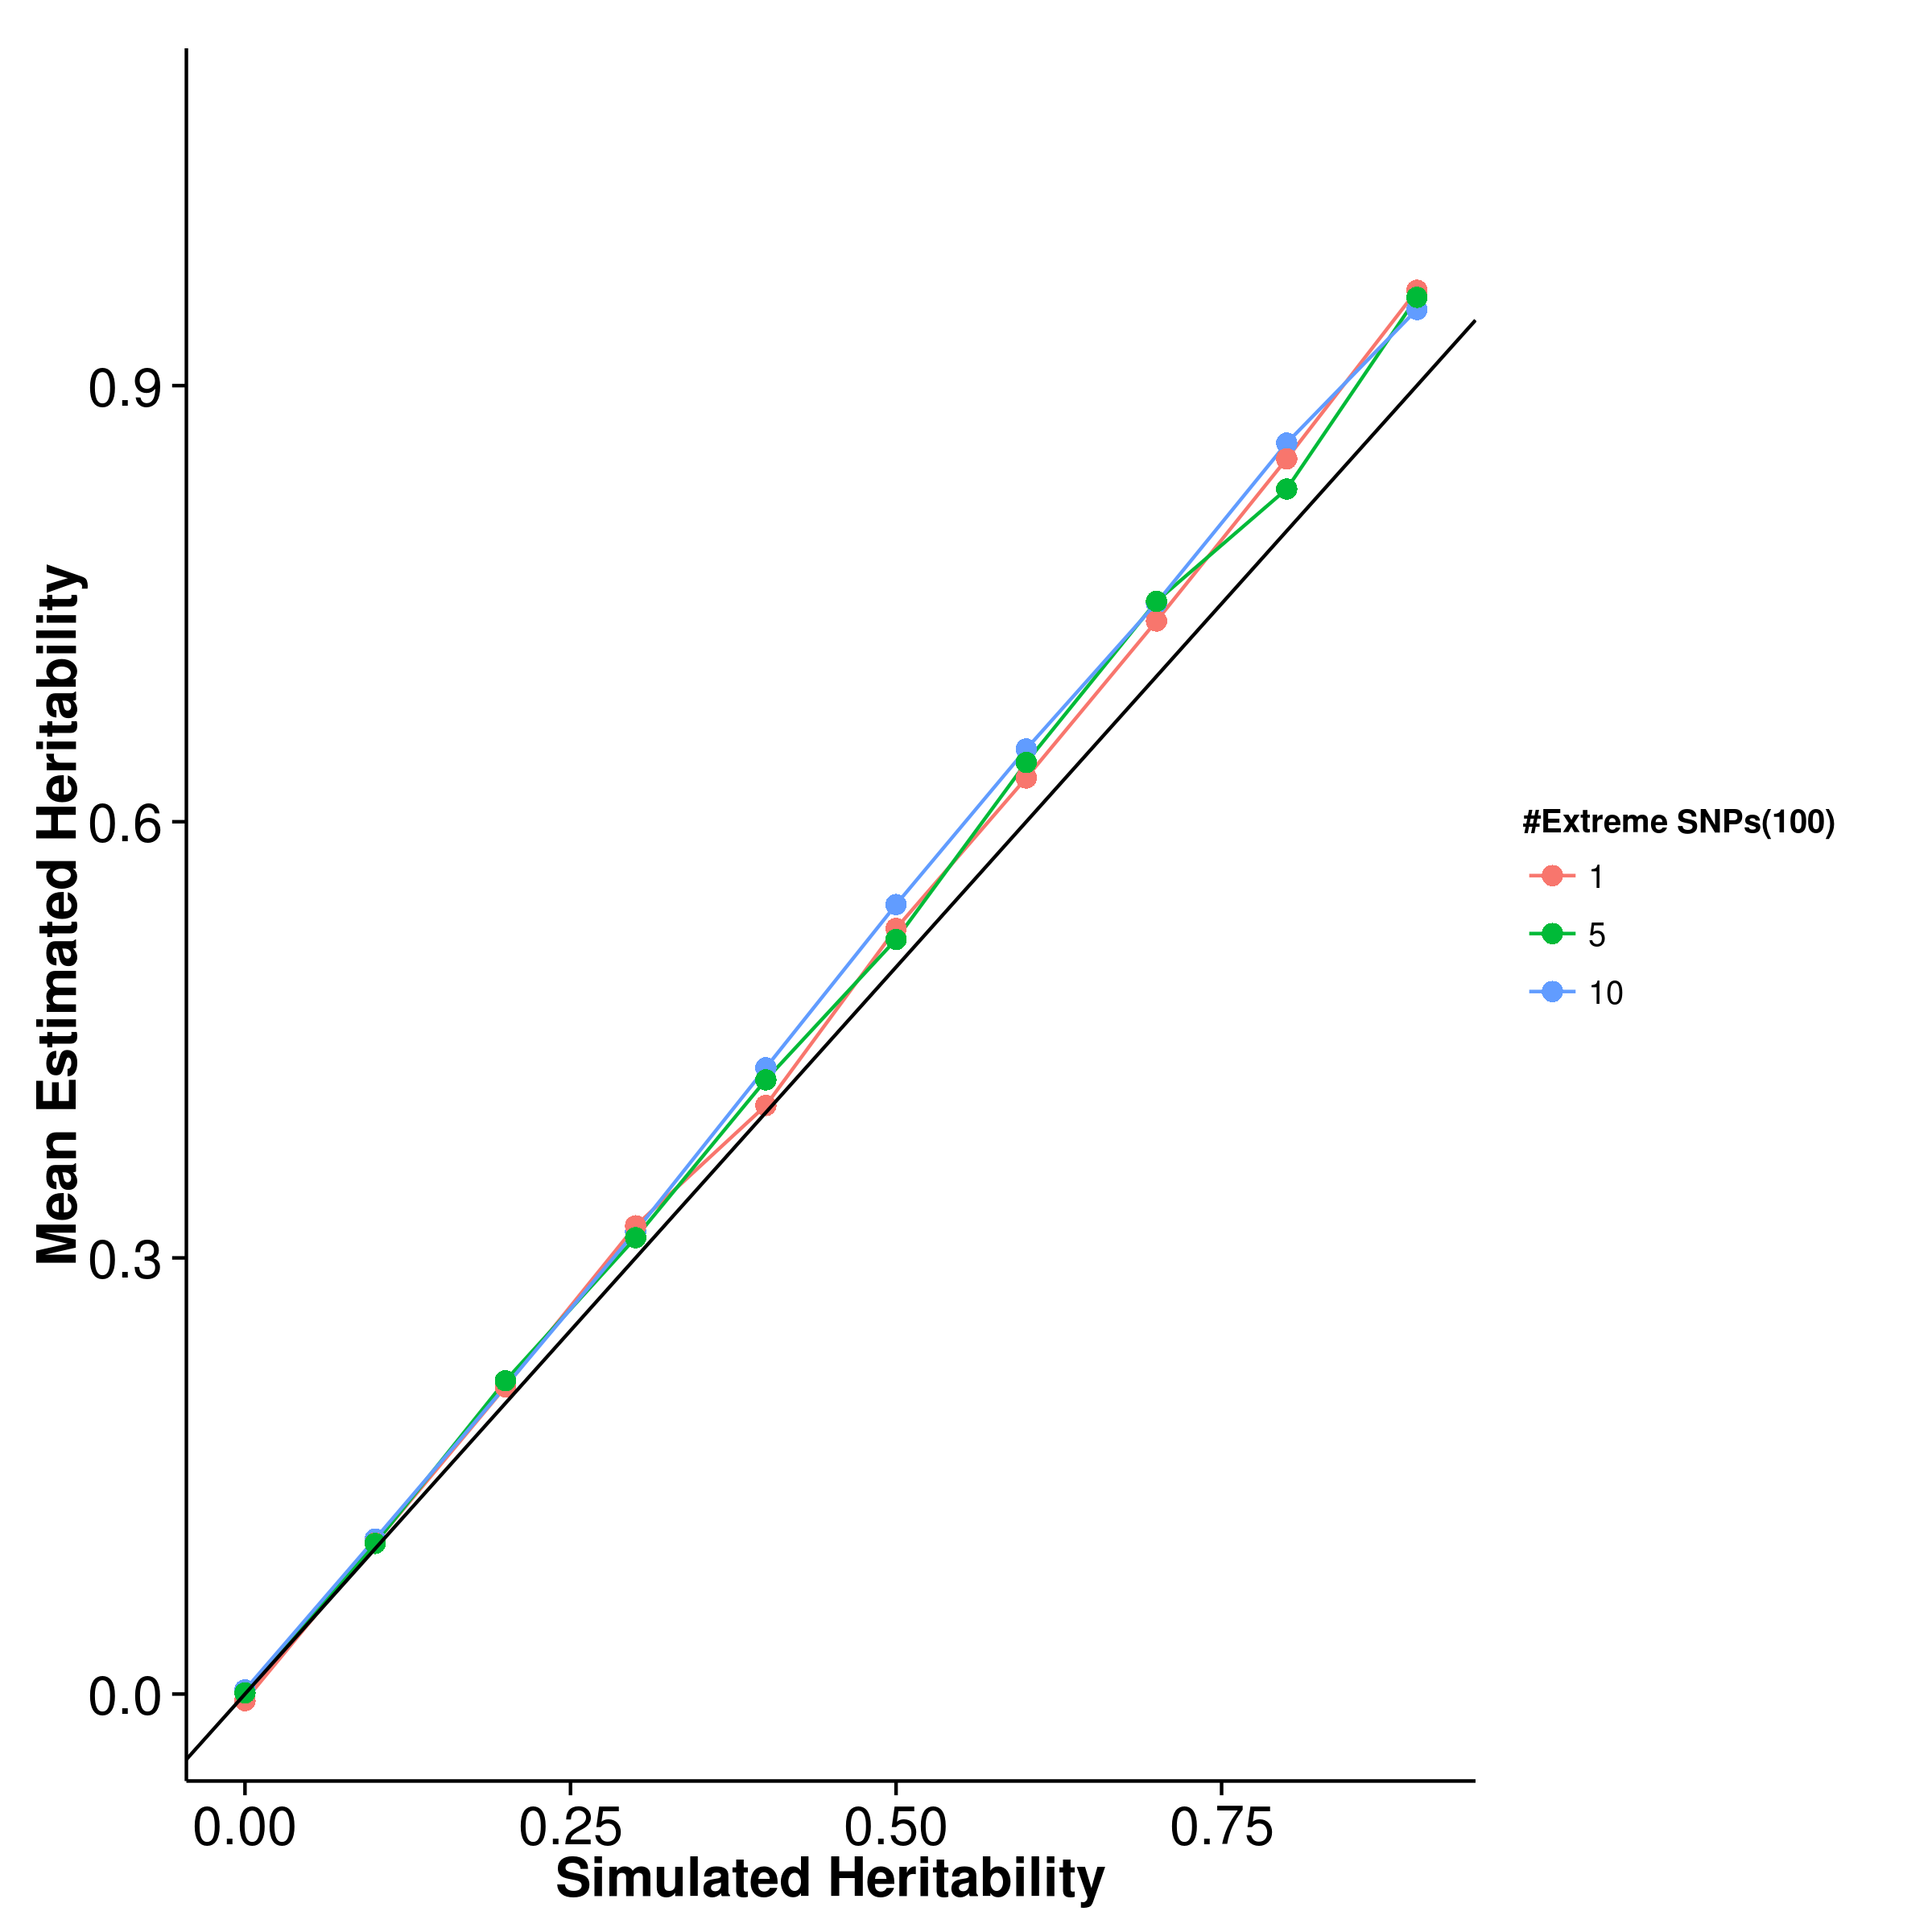
\includegraphics{figure/he_summary/extreme_100c/shrek_QtE_Rand_mean.png}}
				\label{fig:shrekQtEx100cMean}
			}
			\subfloat[GCTA]{
				\scalebox{.4}{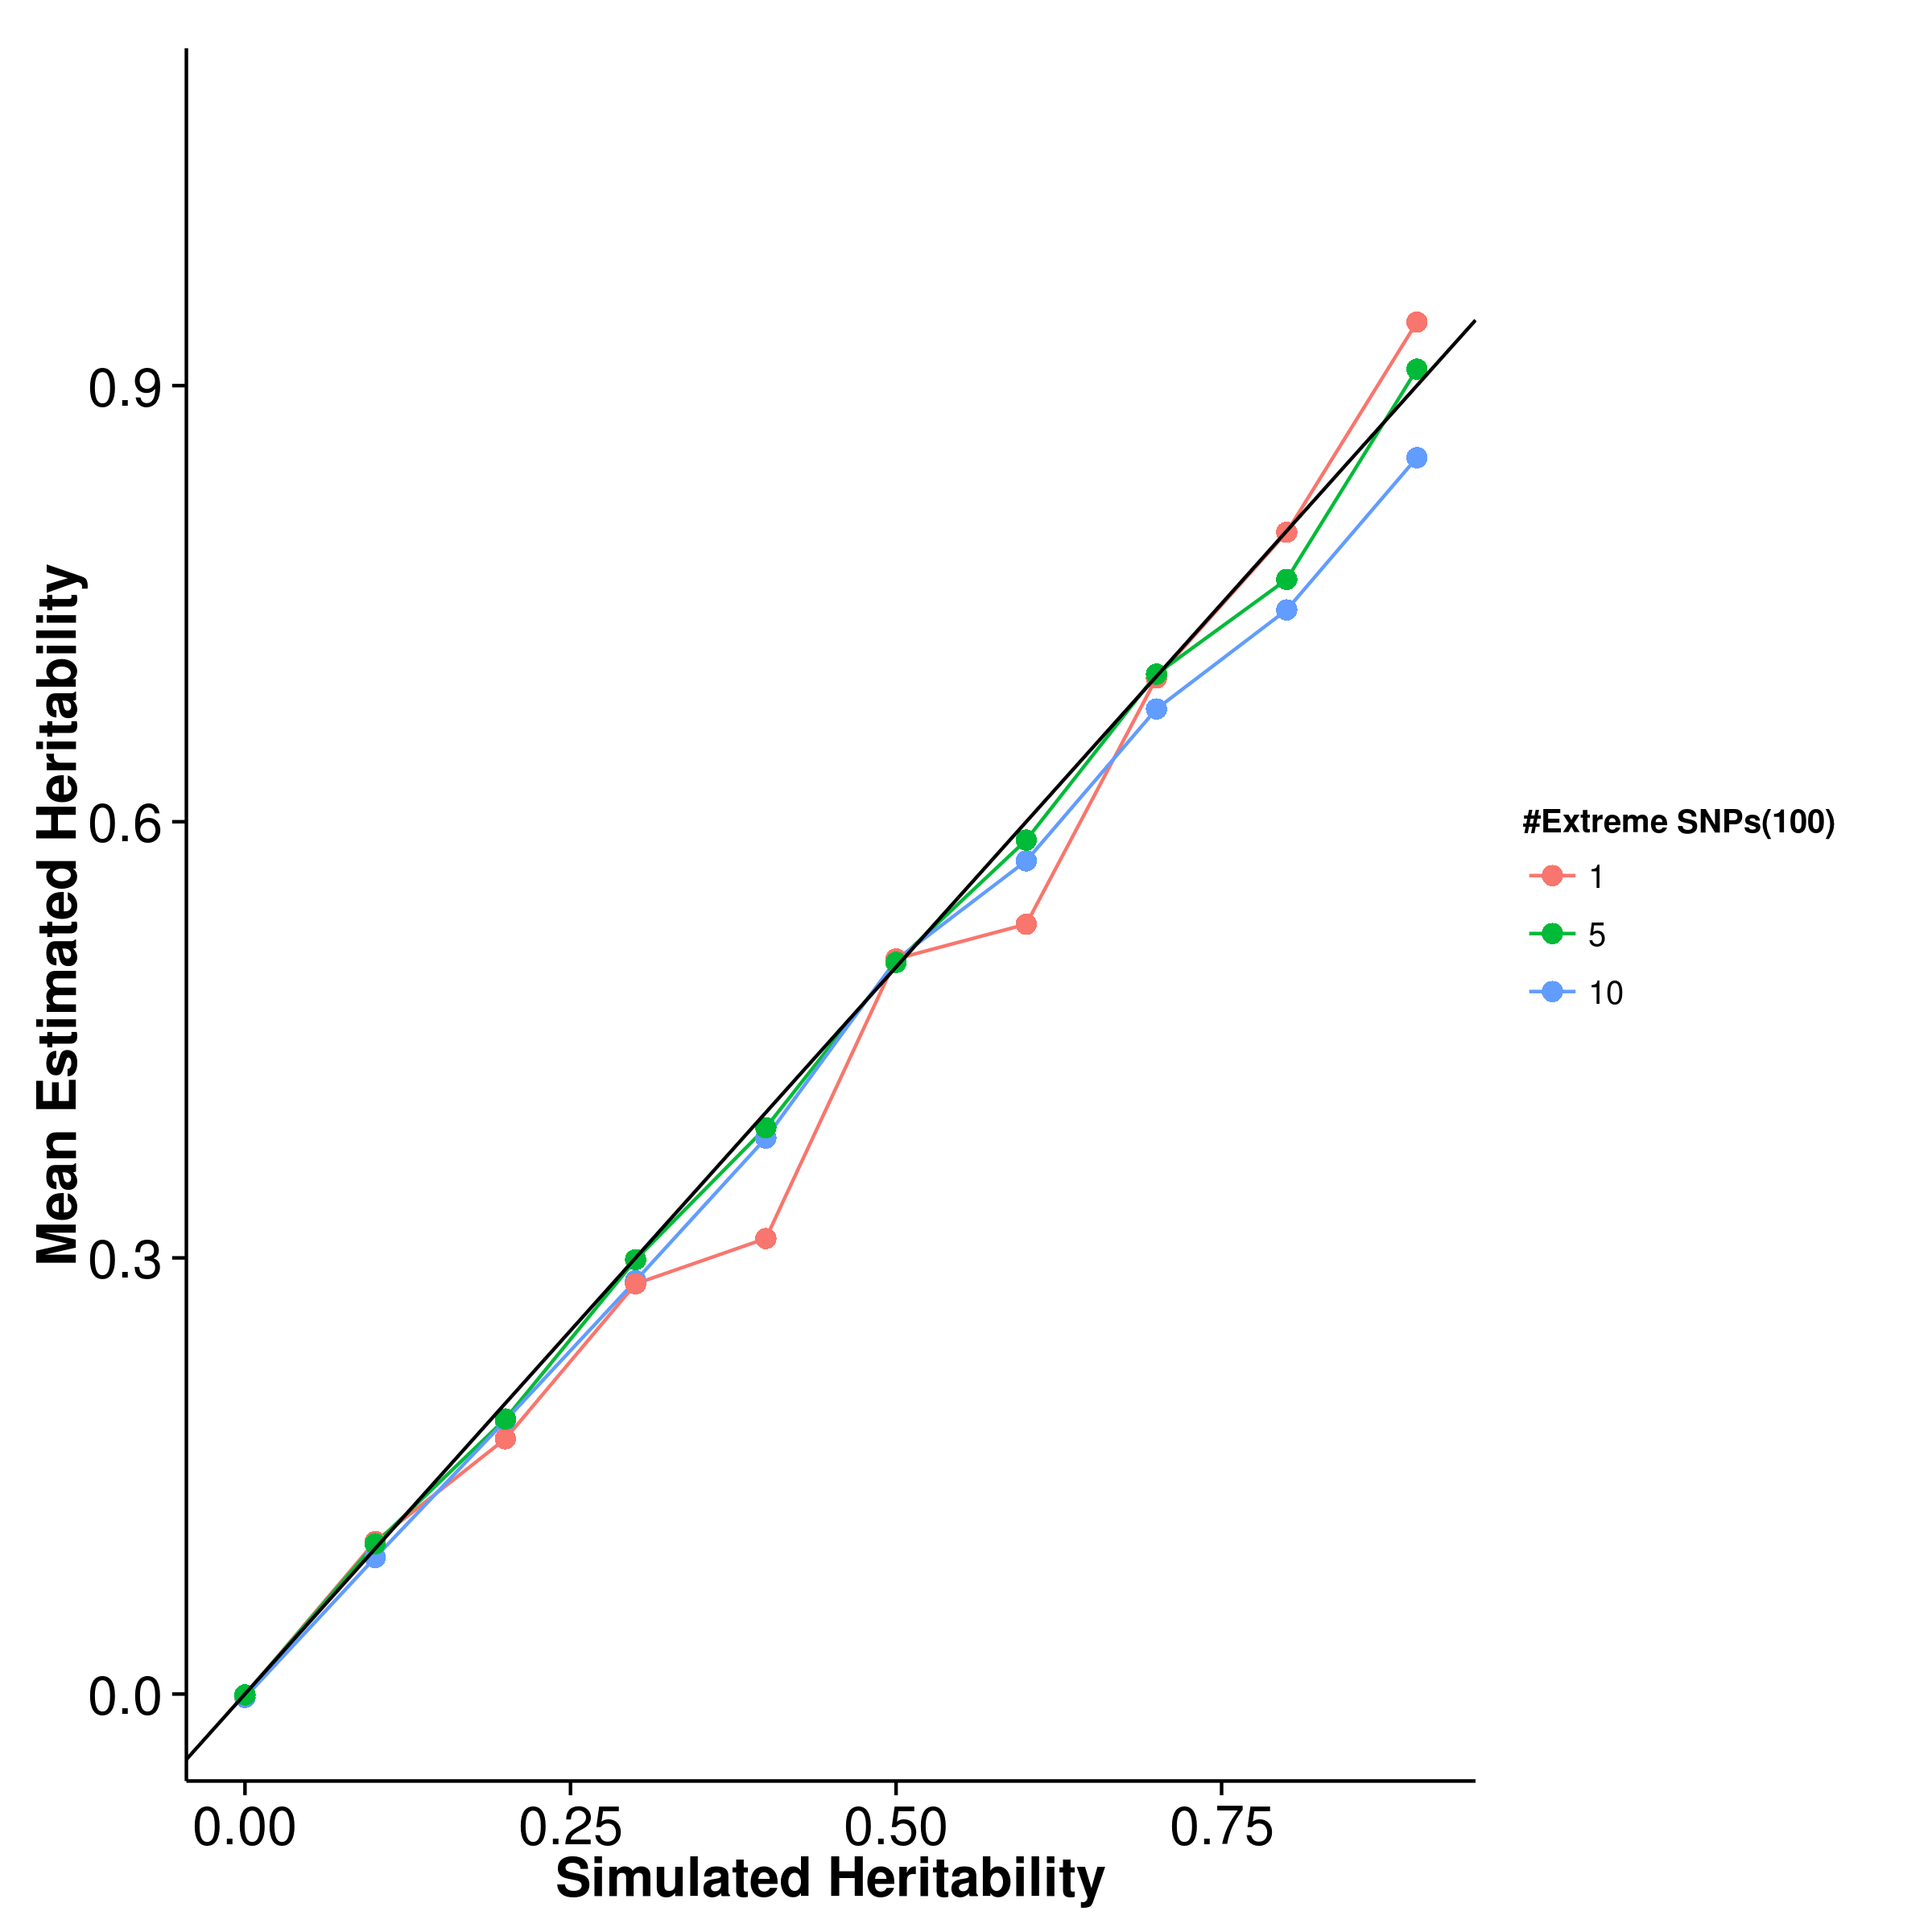
\includegraphics{figure/he_summary/extreme_100c/gcta_QtE_Rand_mean.png}}
				\label{fig:gctaQtEx100cMean}
			}\\
			\subfloat[LDSC with fix intercept]{
				\scalebox{.4}{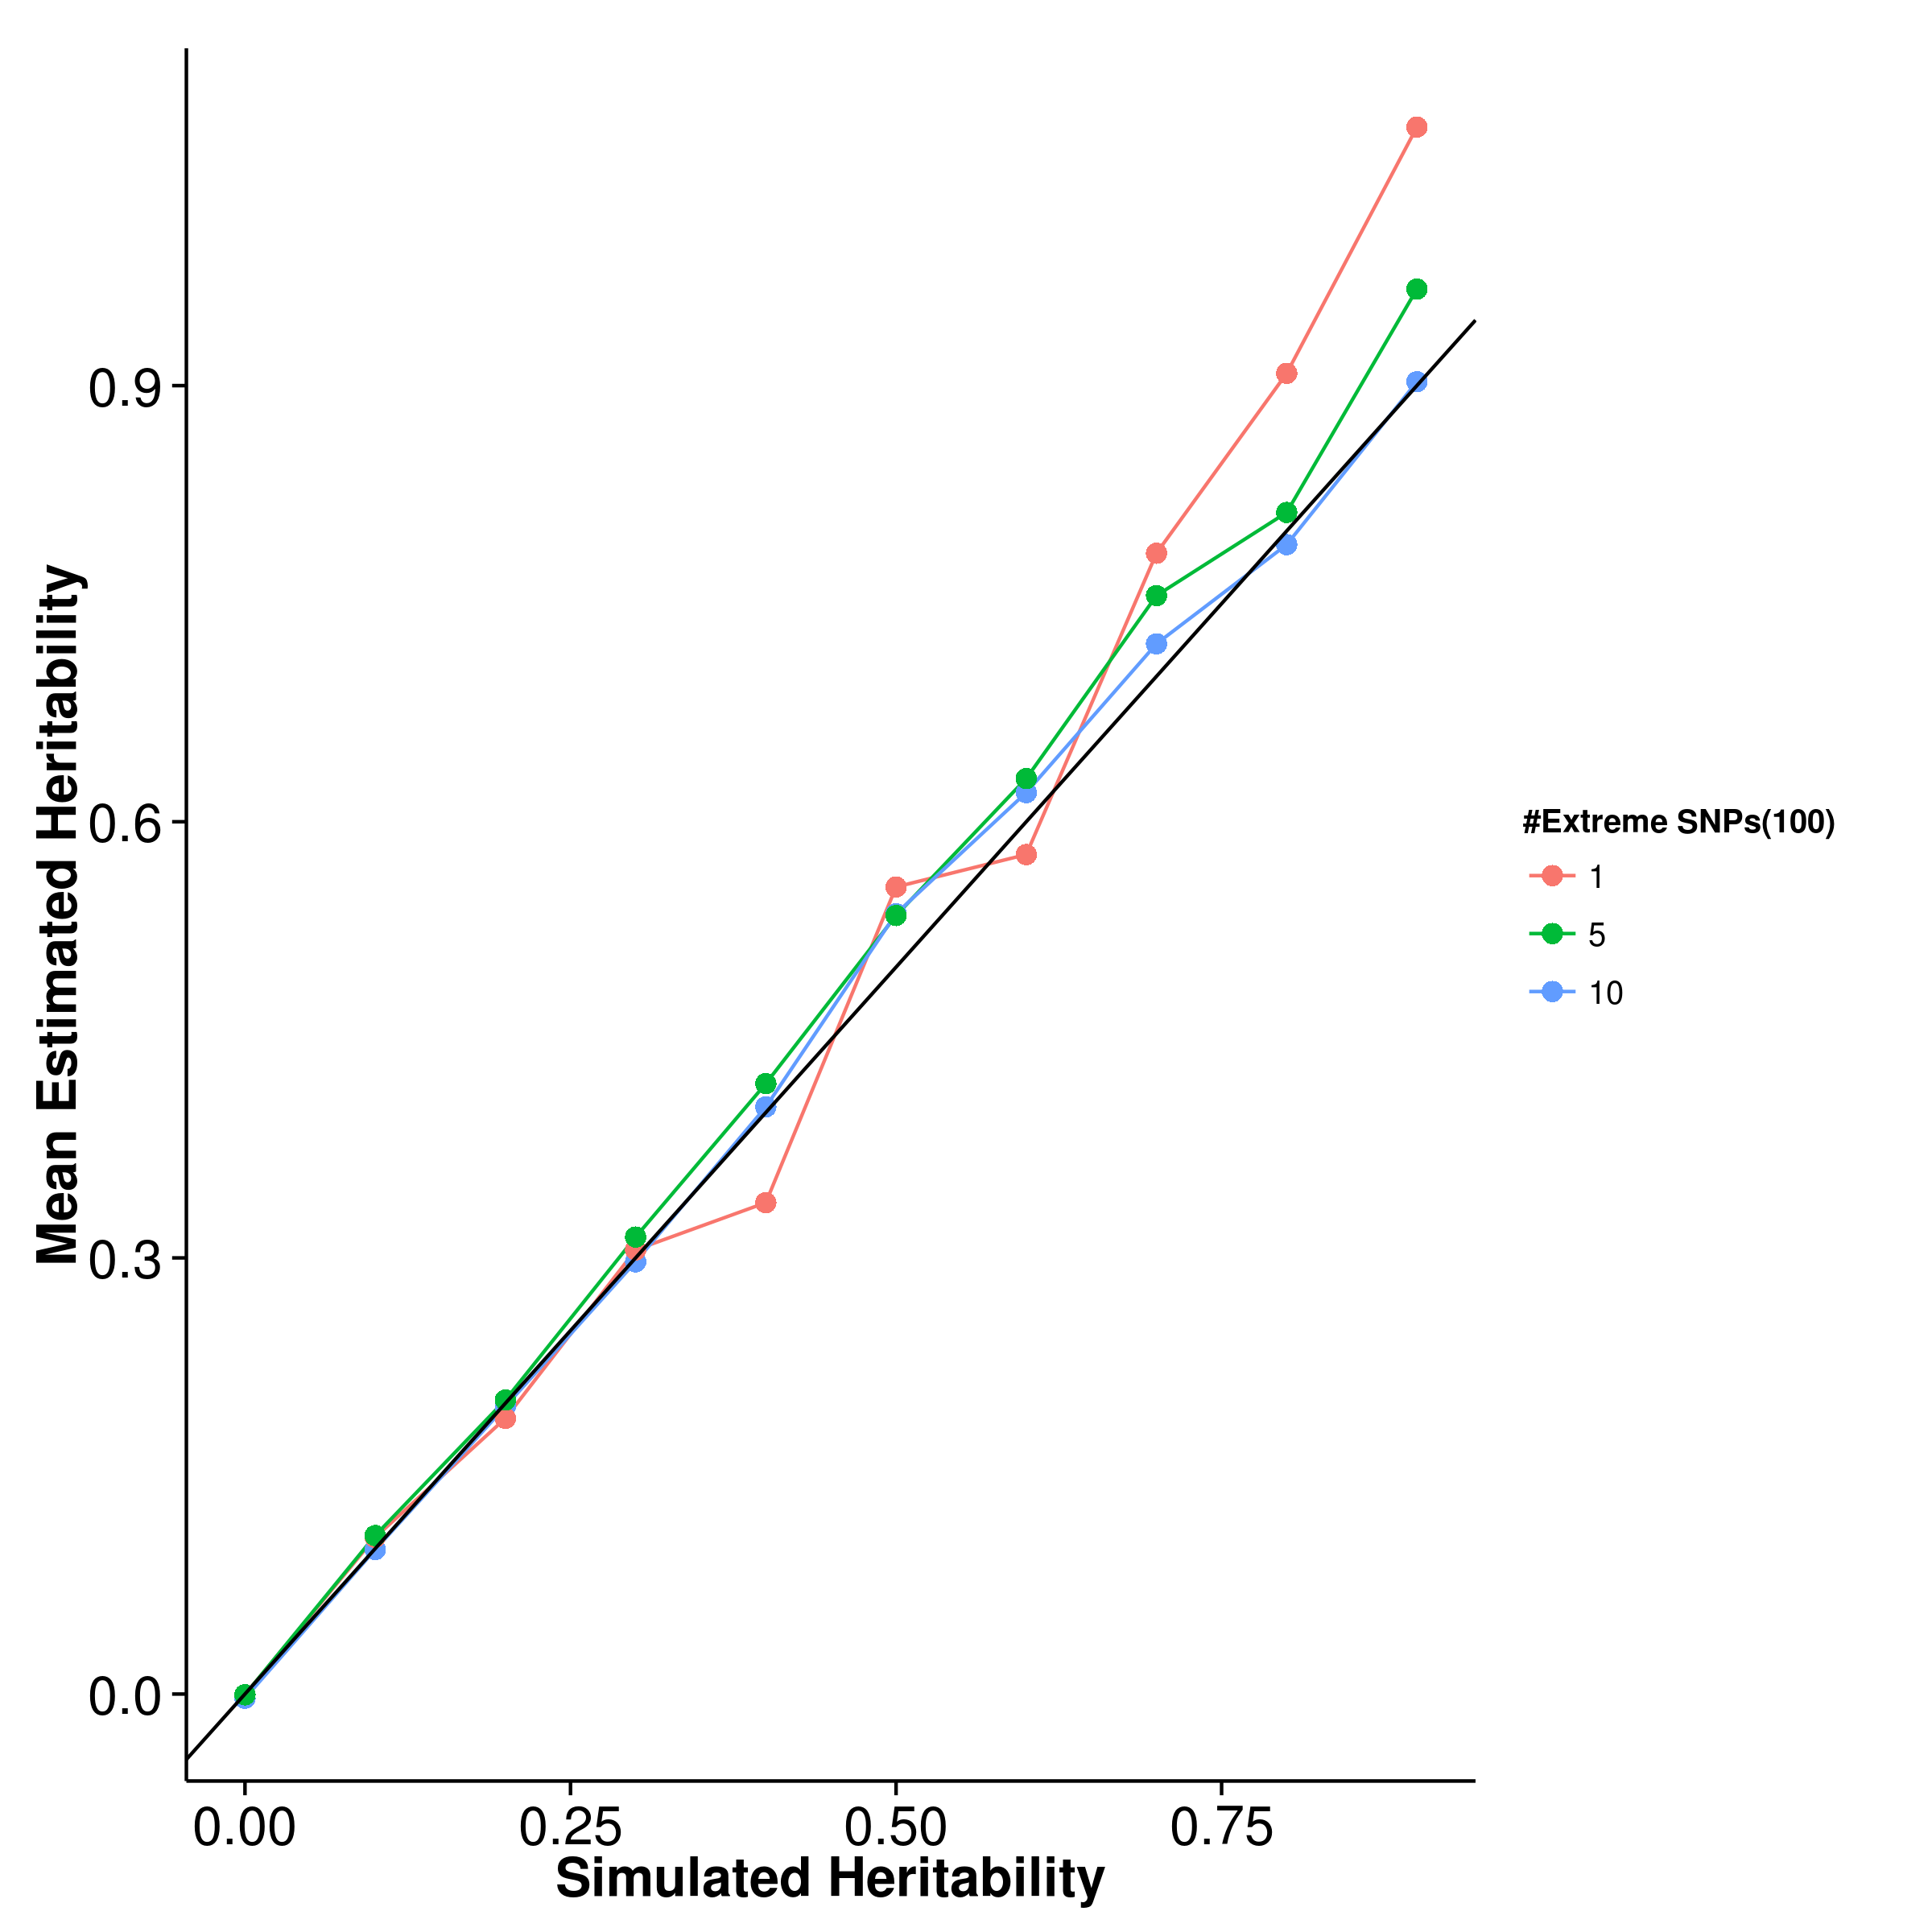
\includegraphics{figure/he_summary/extreme_100c/ldsc_QtE_Rand_mean.png}}
				\label{fig:ldscQtEx100cMean}
			}
			\subfloat[LDSC with intercept estimation]{
				
				\scalebox{.4}{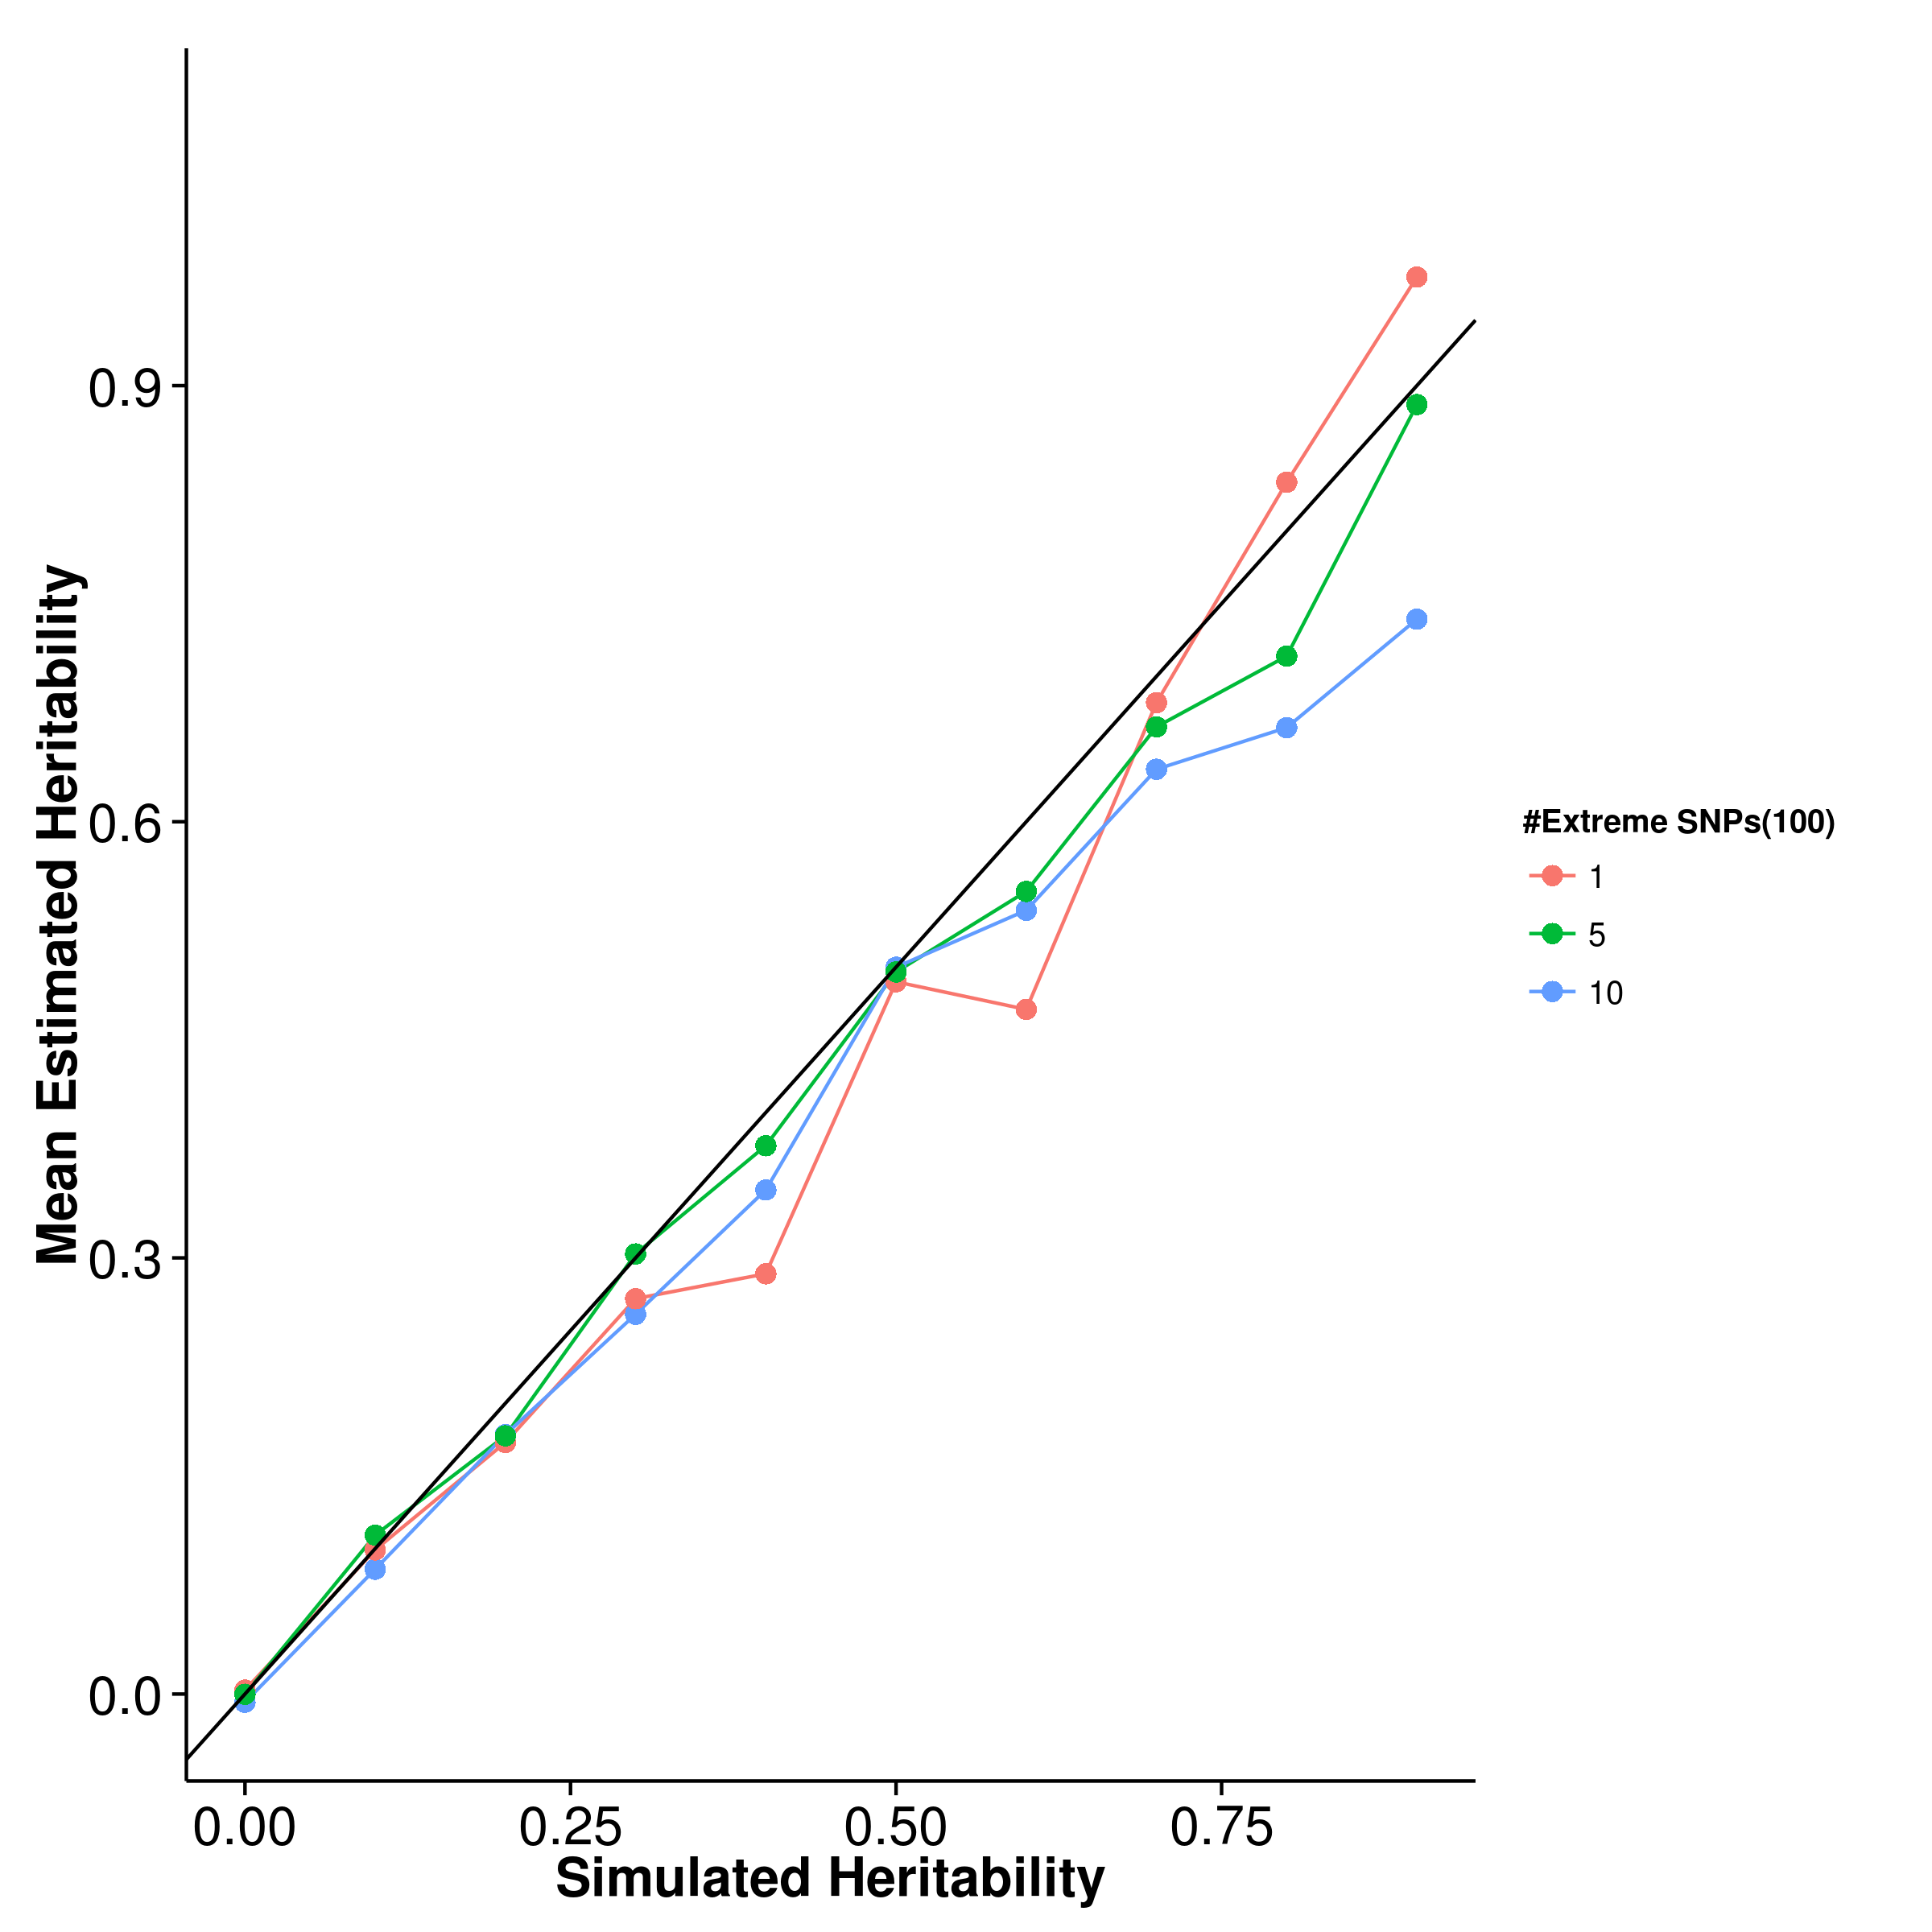
\includegraphics{figure/he_summary/extreme_100c/ldscIn_QtE_Rand_mean.png}}
				\label{fig:ldscInQtEx100cMean}
			}
			\caption[Mean of Extreme Effect Size Simulation Result]
			{Mean of results from quantitative trait simulation with extreme effect size simulation.
				It was observed that the mean estimation of heritability of \gls{shrek} is not affected by the number of \gls{SNP}(s) with large effect but with slight upward bias.
				On the other hand, the mean estimation of \gls{ldsc} and \gls{gcta} seems to fluctuate with respect to the simulated heritability.
				} 
			\label{fig:QtEx100cMean}
		\end{figure}
		
		\begin{figure}
			\centering
			\subfloat[SHREK]{
				\scalebox{.4}{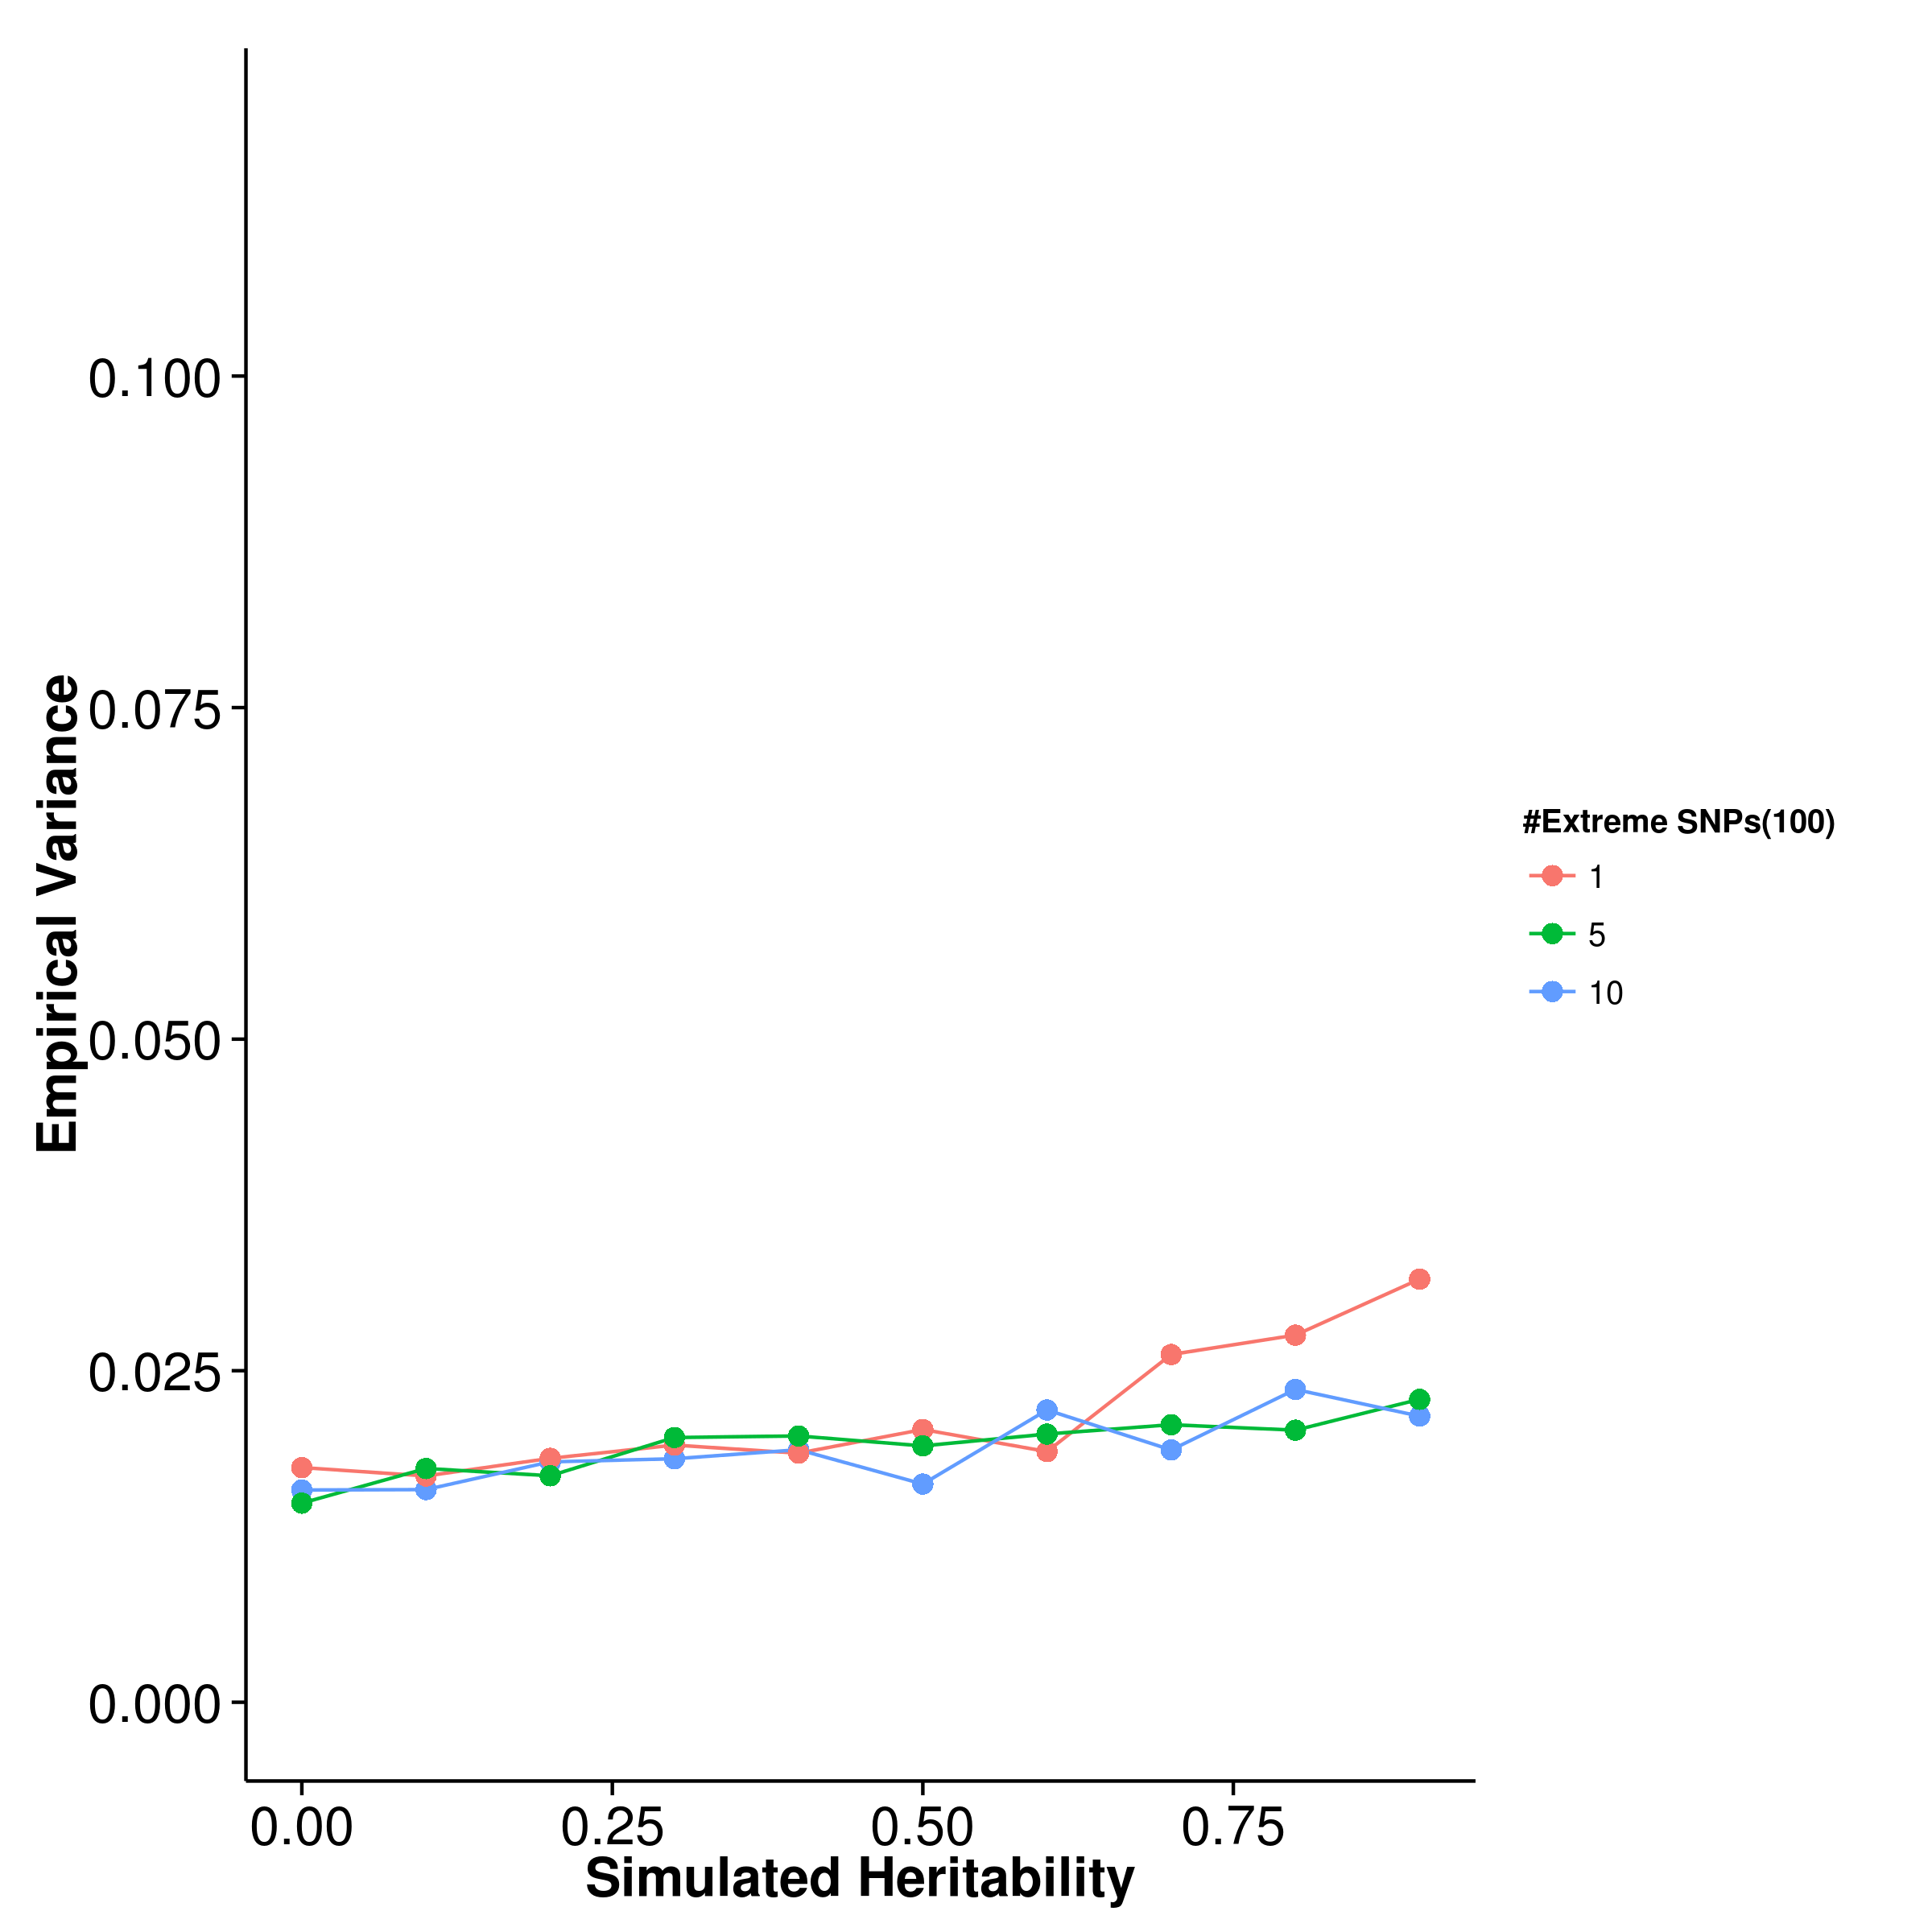
\includegraphics{figure/he_summary/extreme_100c/shrek_QtE_Rand_sd.png}}
				\label{fig:shrekQtEx100cVar}
			}
			\subfloat[GCTA]{
				\scalebox{.4}{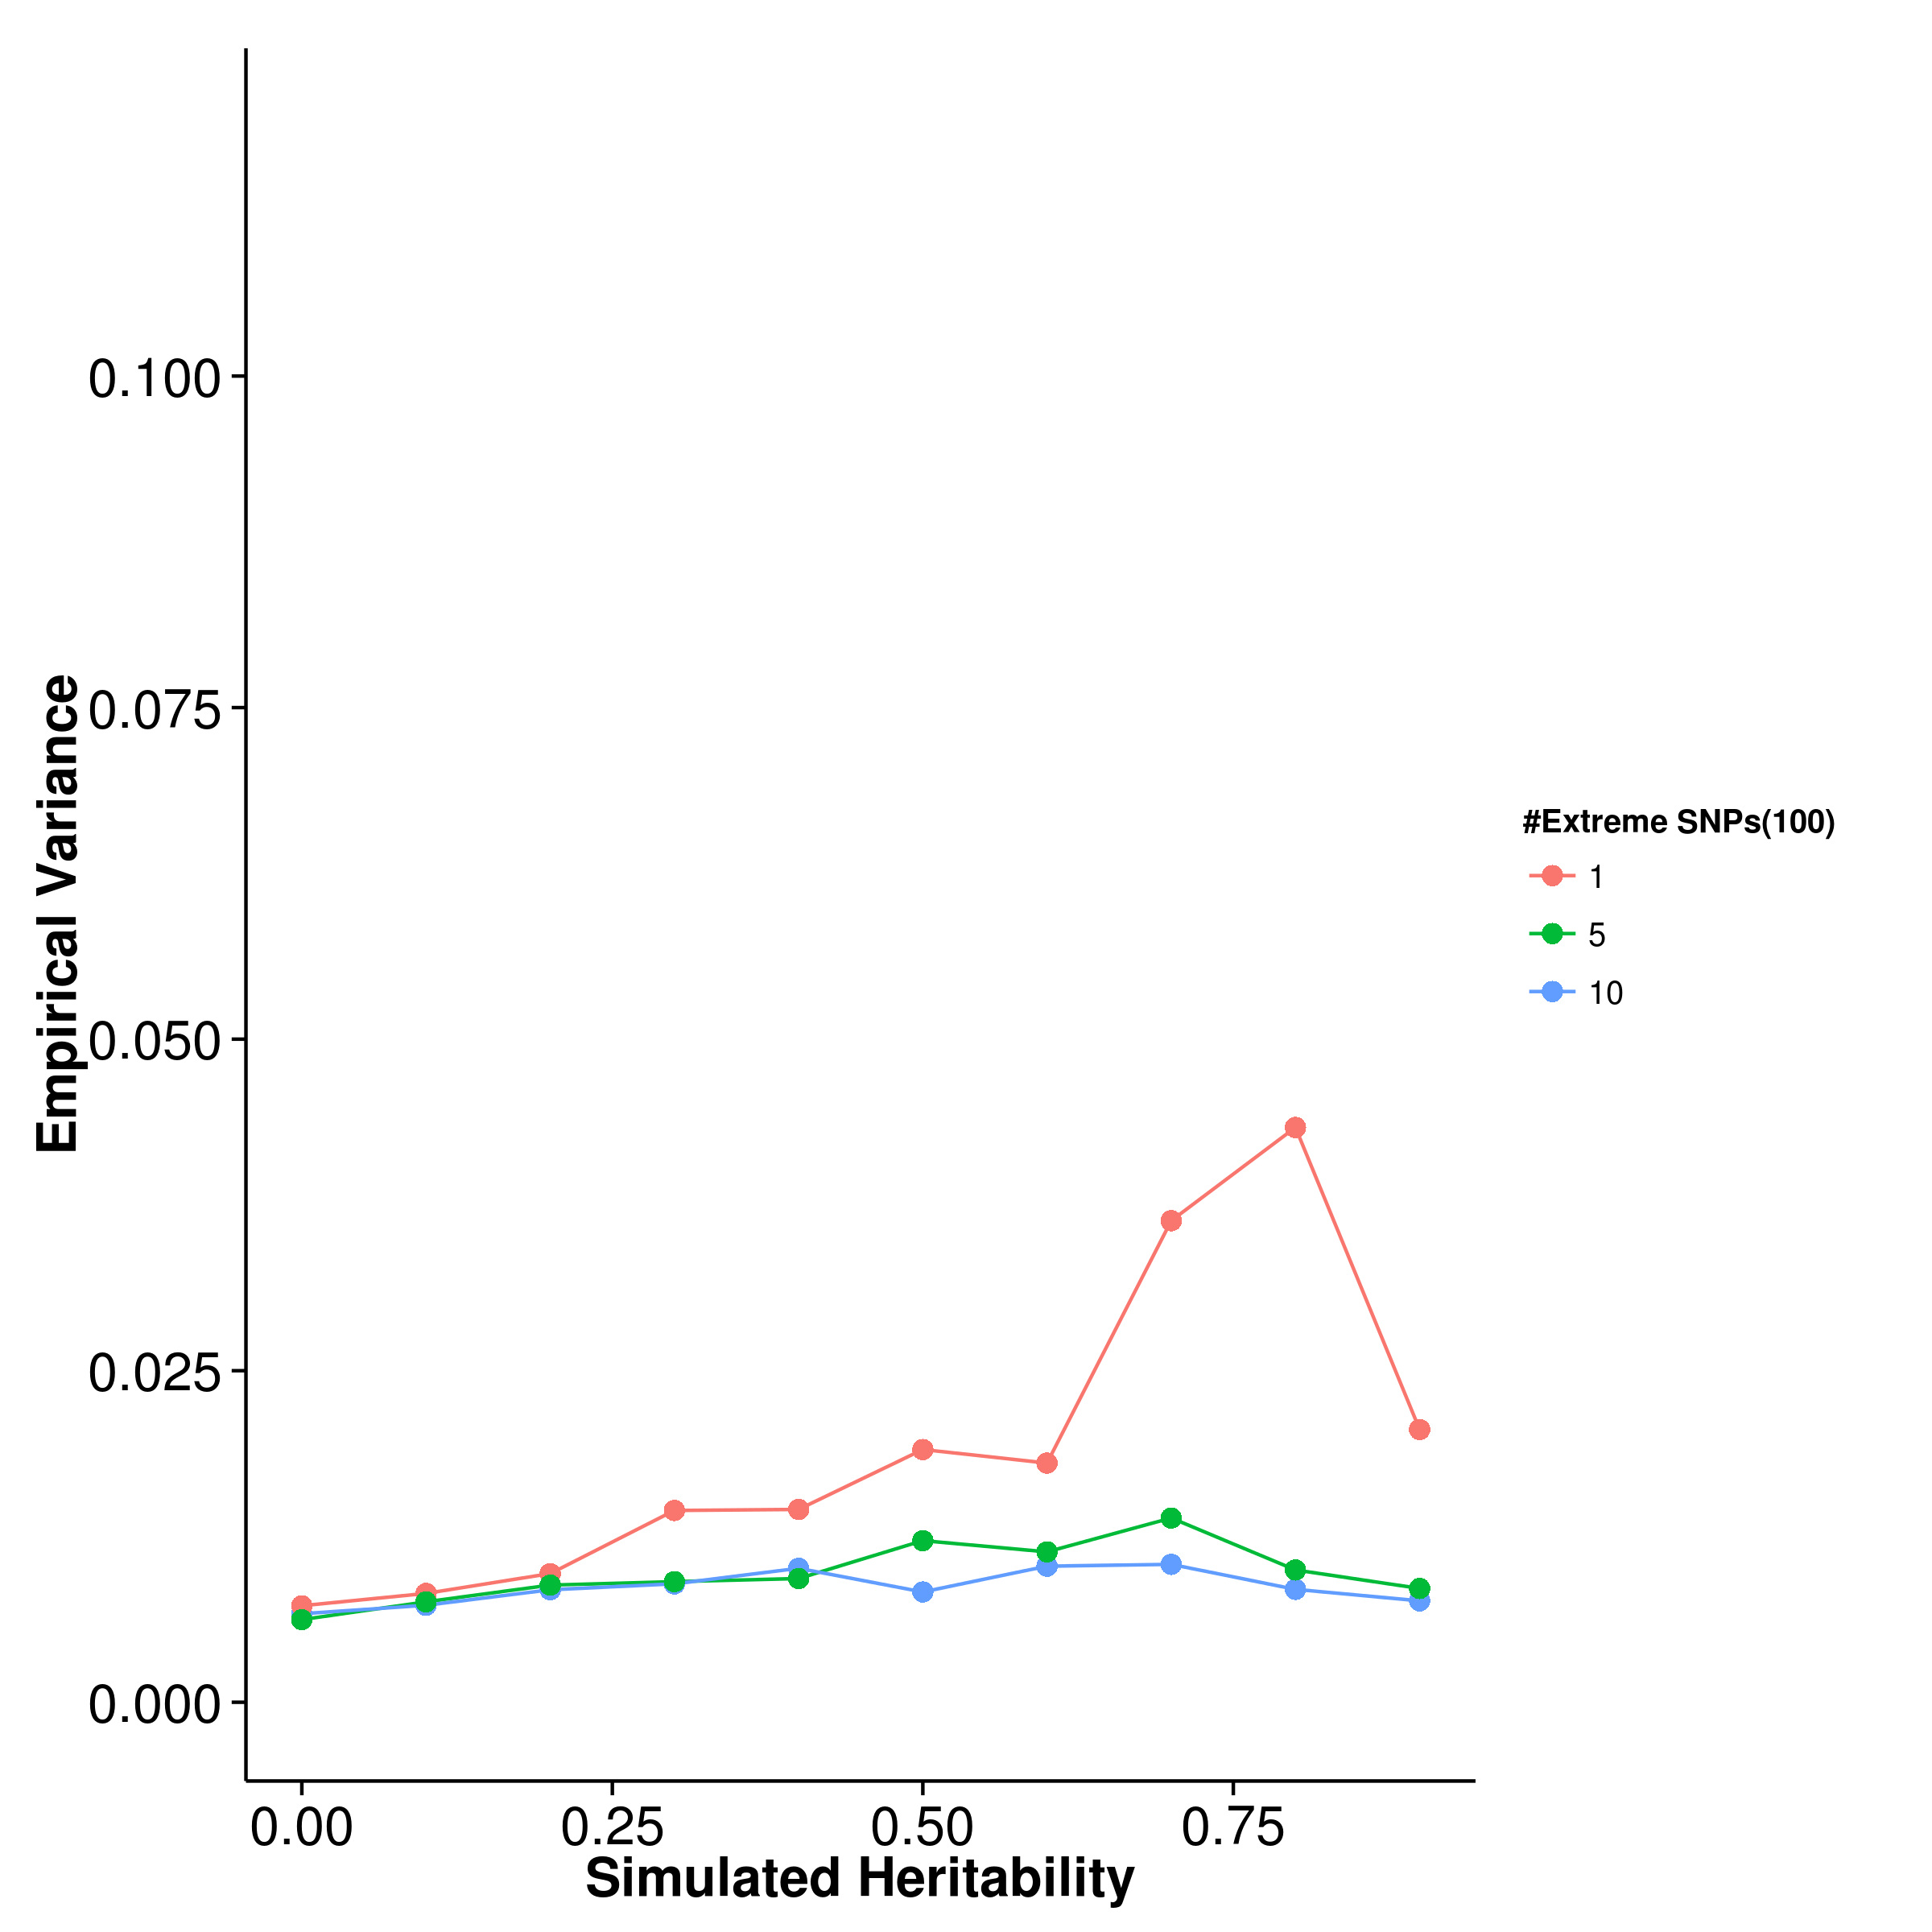
\includegraphics{figure/he_summary/extreme_100c/gcta_QtE_Rand_sd.png}}
				\label{fig:gctaQtEx100cVar}
			}\\
			\subfloat[LDSC with fix intercept]{
				\scalebox{.4}{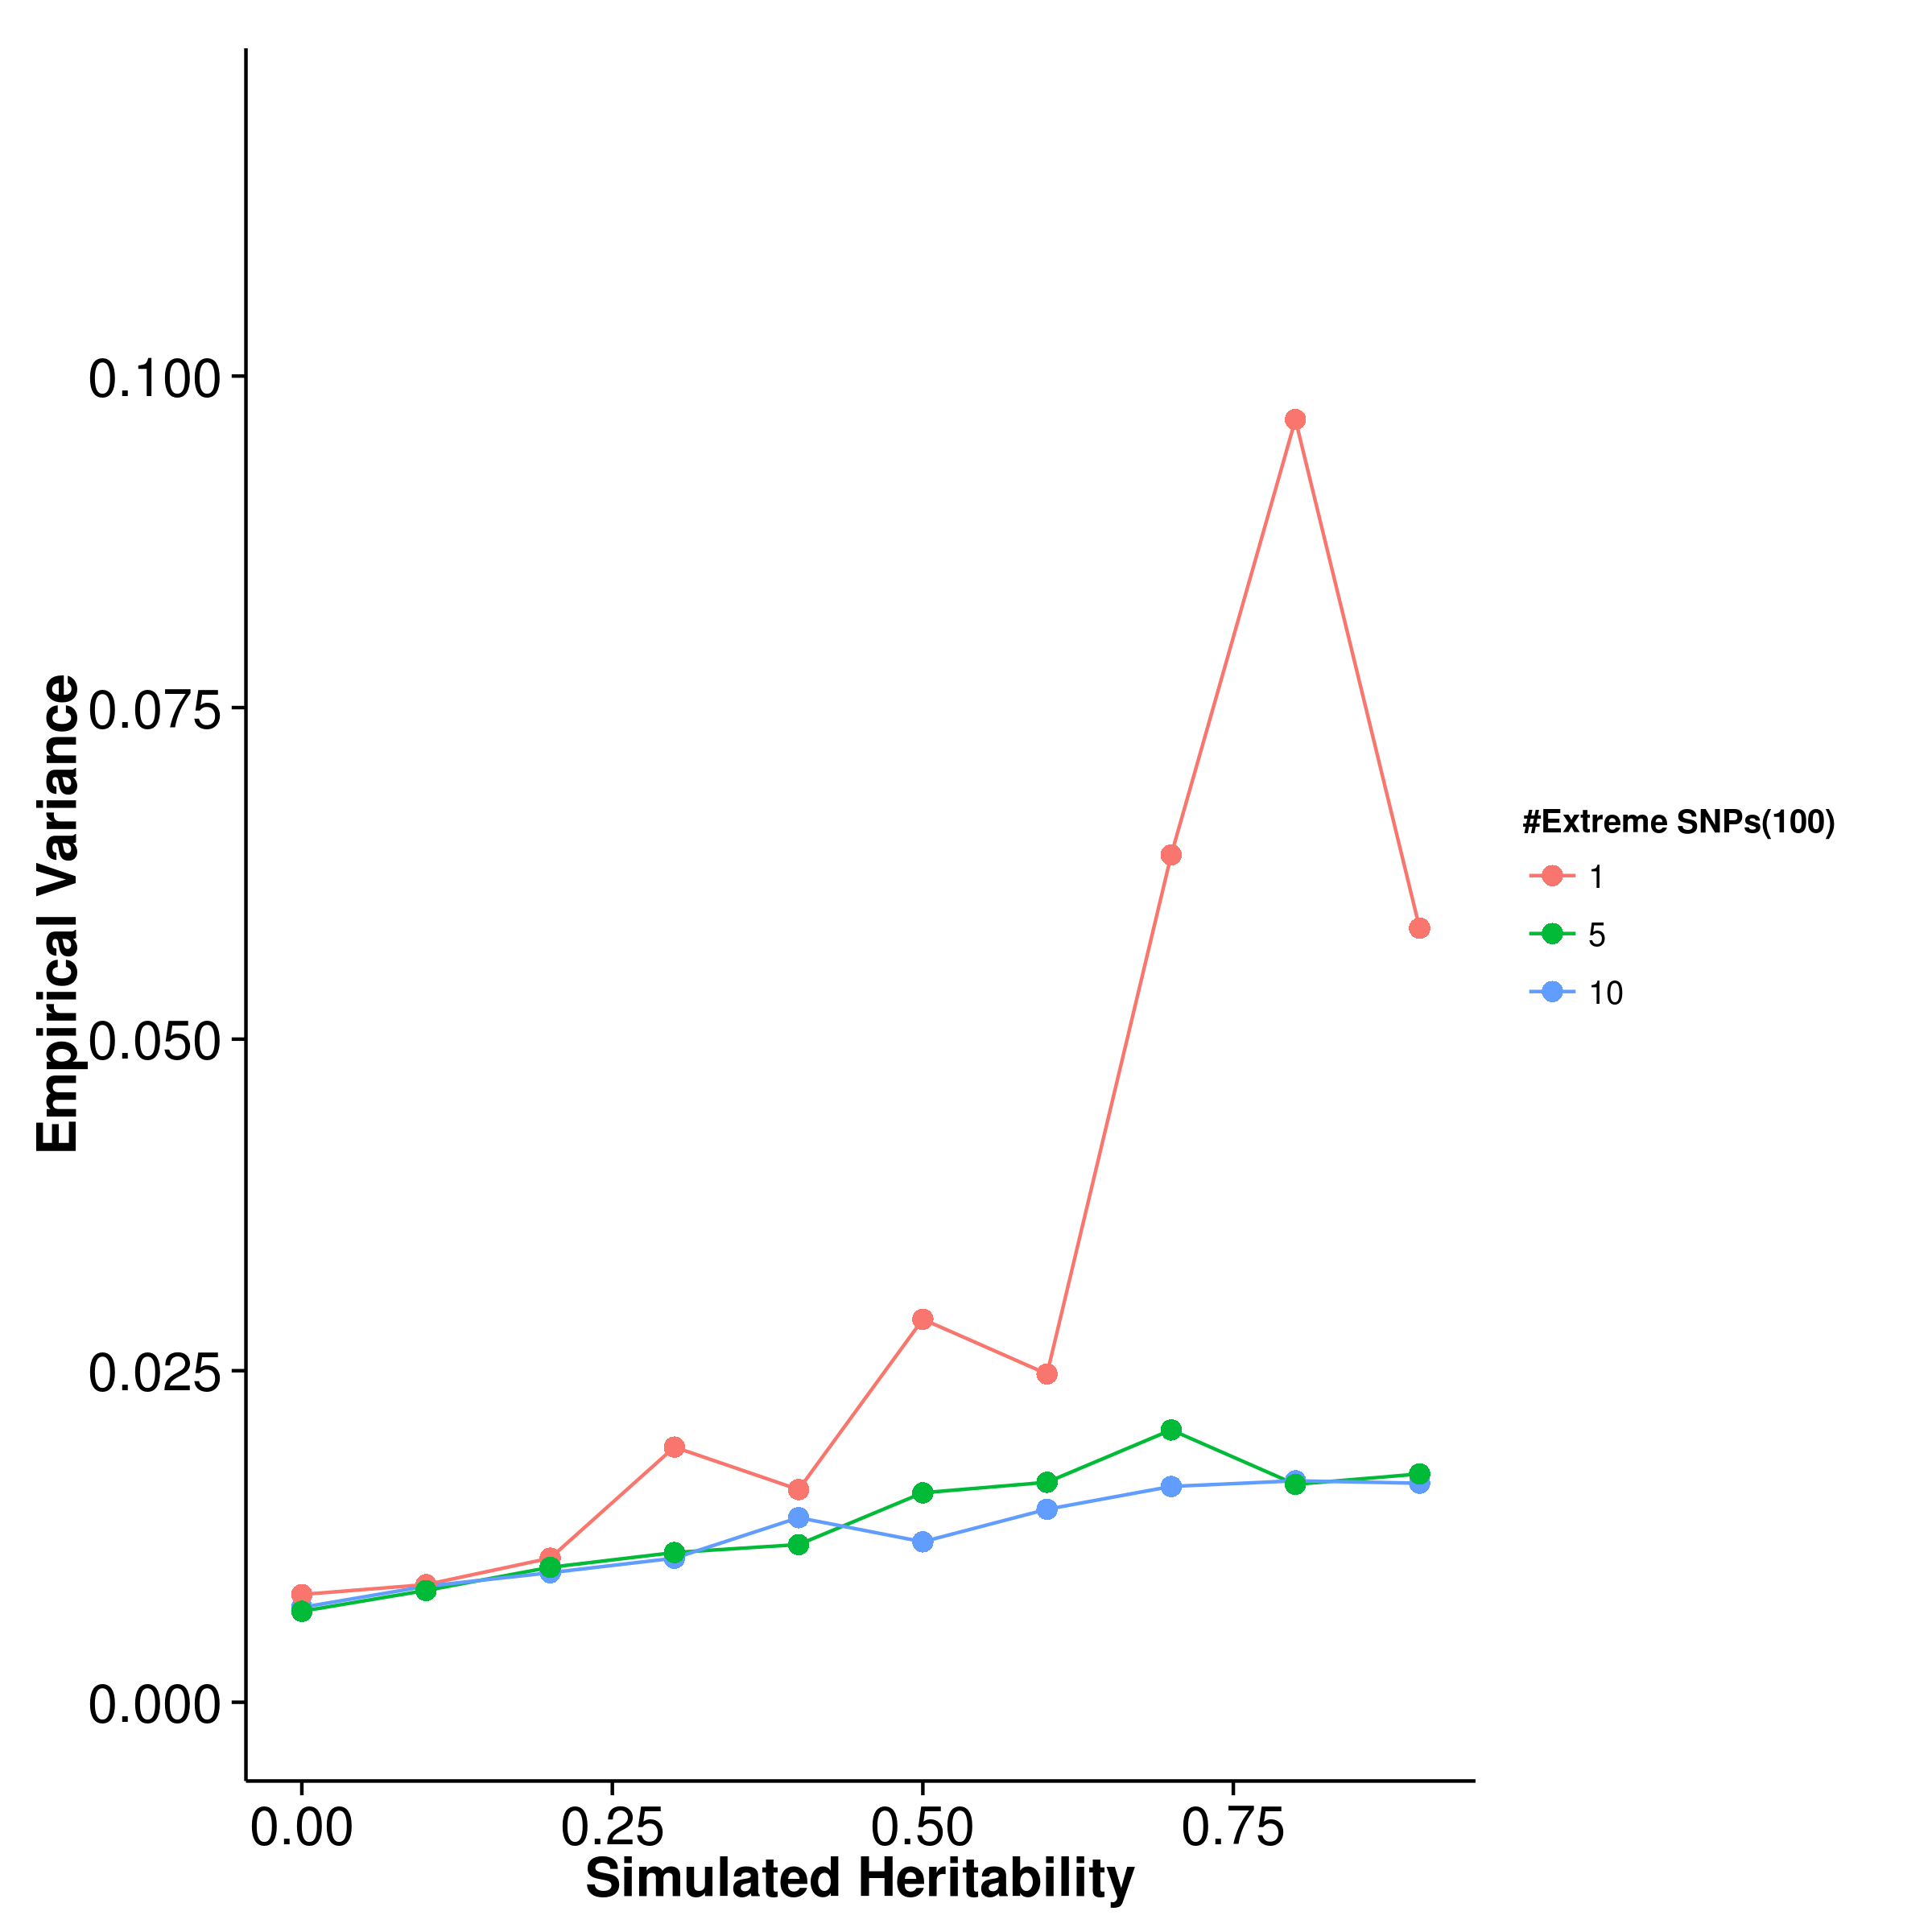
\includegraphics{figure/he_summary/extreme_100c/ldsc_QtE_Rand_sd.png}}
				\label{fig:ldscQtEx100cVar}
			}
			\subfloat[LDSC with intercept estimation]{
				
				\scalebox{.4}{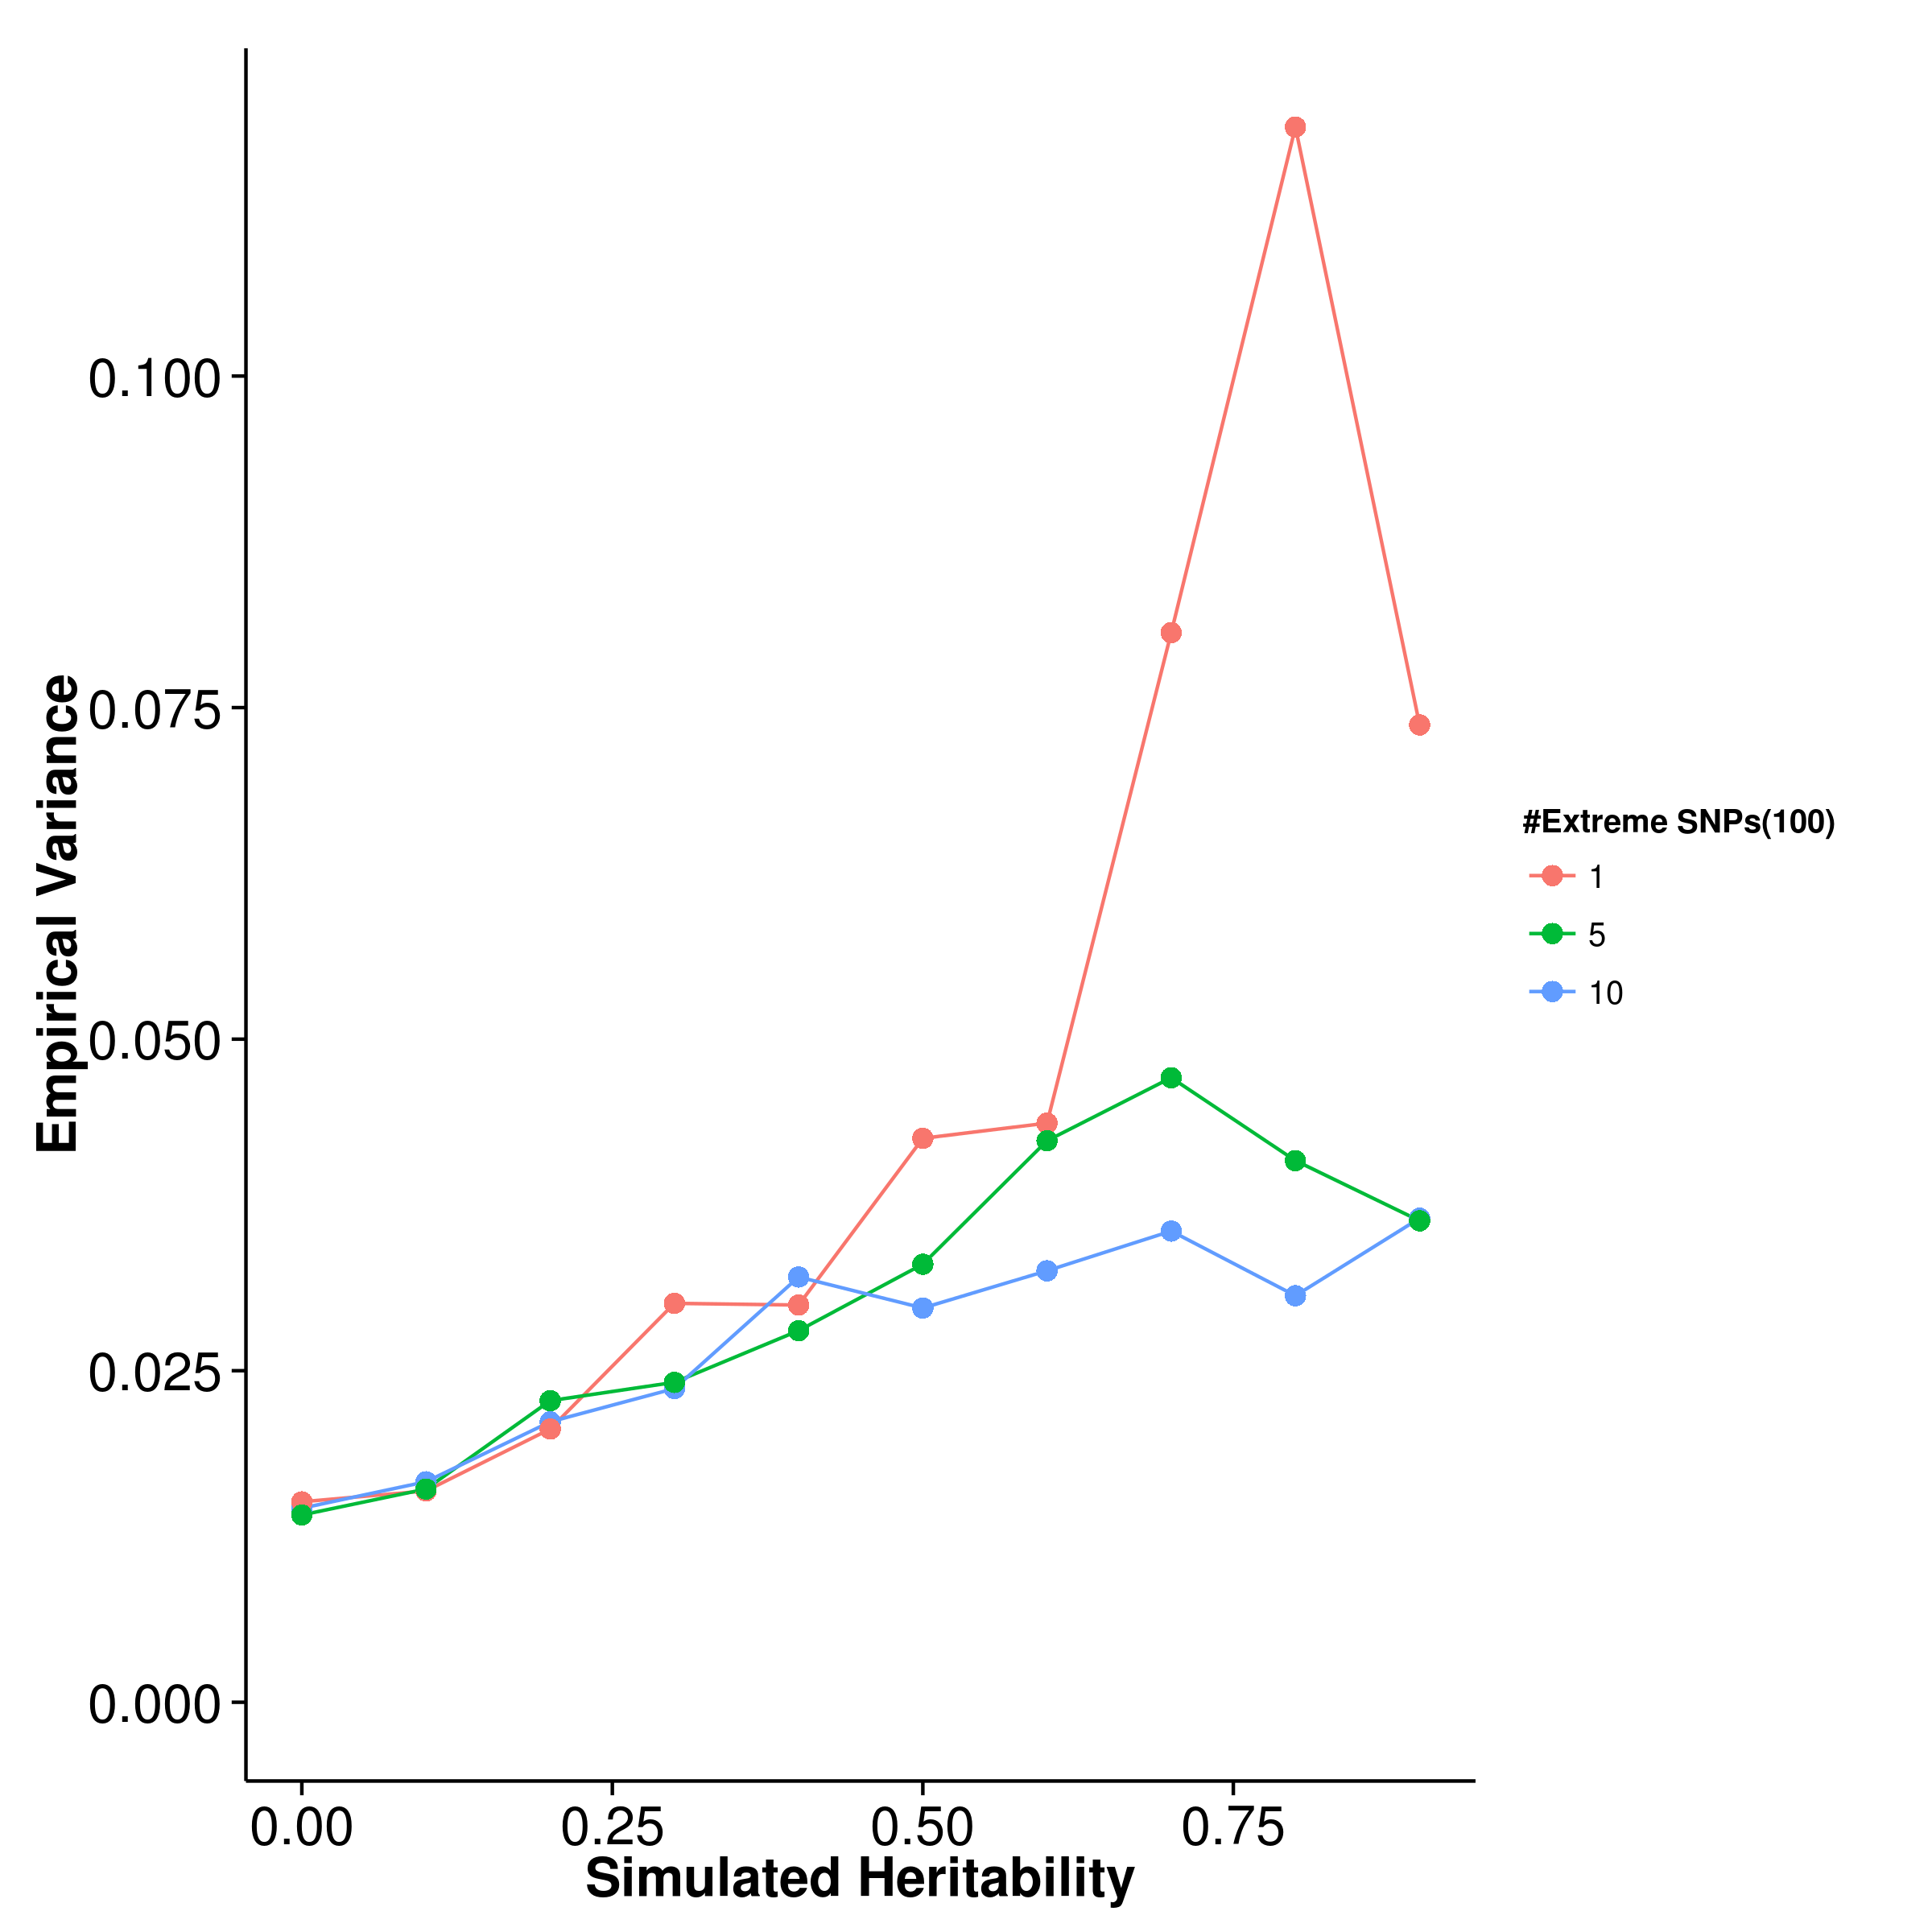
\includegraphics{figure/he_summary/extreme_100c/ldscIn_QtE_Rand_sd.png}}
				\label{fig:ldscInQtEx100cVar}
			}
			\caption[Variance of Extreme Effect Size Simulation Result]
			{Variance of results from quantitative trait simulation with extreme effect size simulation.
				100 causal \glspl{SNP} were simulated.
				When only 1 \gls{SNP} with extreme effect was simulated, the empirical variance of \gls{gcta} and \gls{ldsc} increases and a large fluctuation was observed.
				Whereas the empirical variance of \gls{shrek} only increase slightly when the simulated heritability is large and with only 1 \gls{SNP} with extreme effect.
				Suggesting that it is more robust to the change in number of extreme \gls{SNP}(s).
			} 
			\label{fig:QtEx100cVar}
		\end{figure}
		
		\begin{figure}
			\centering
			\subfloat[SHREK]{
				\scalebox{.4}{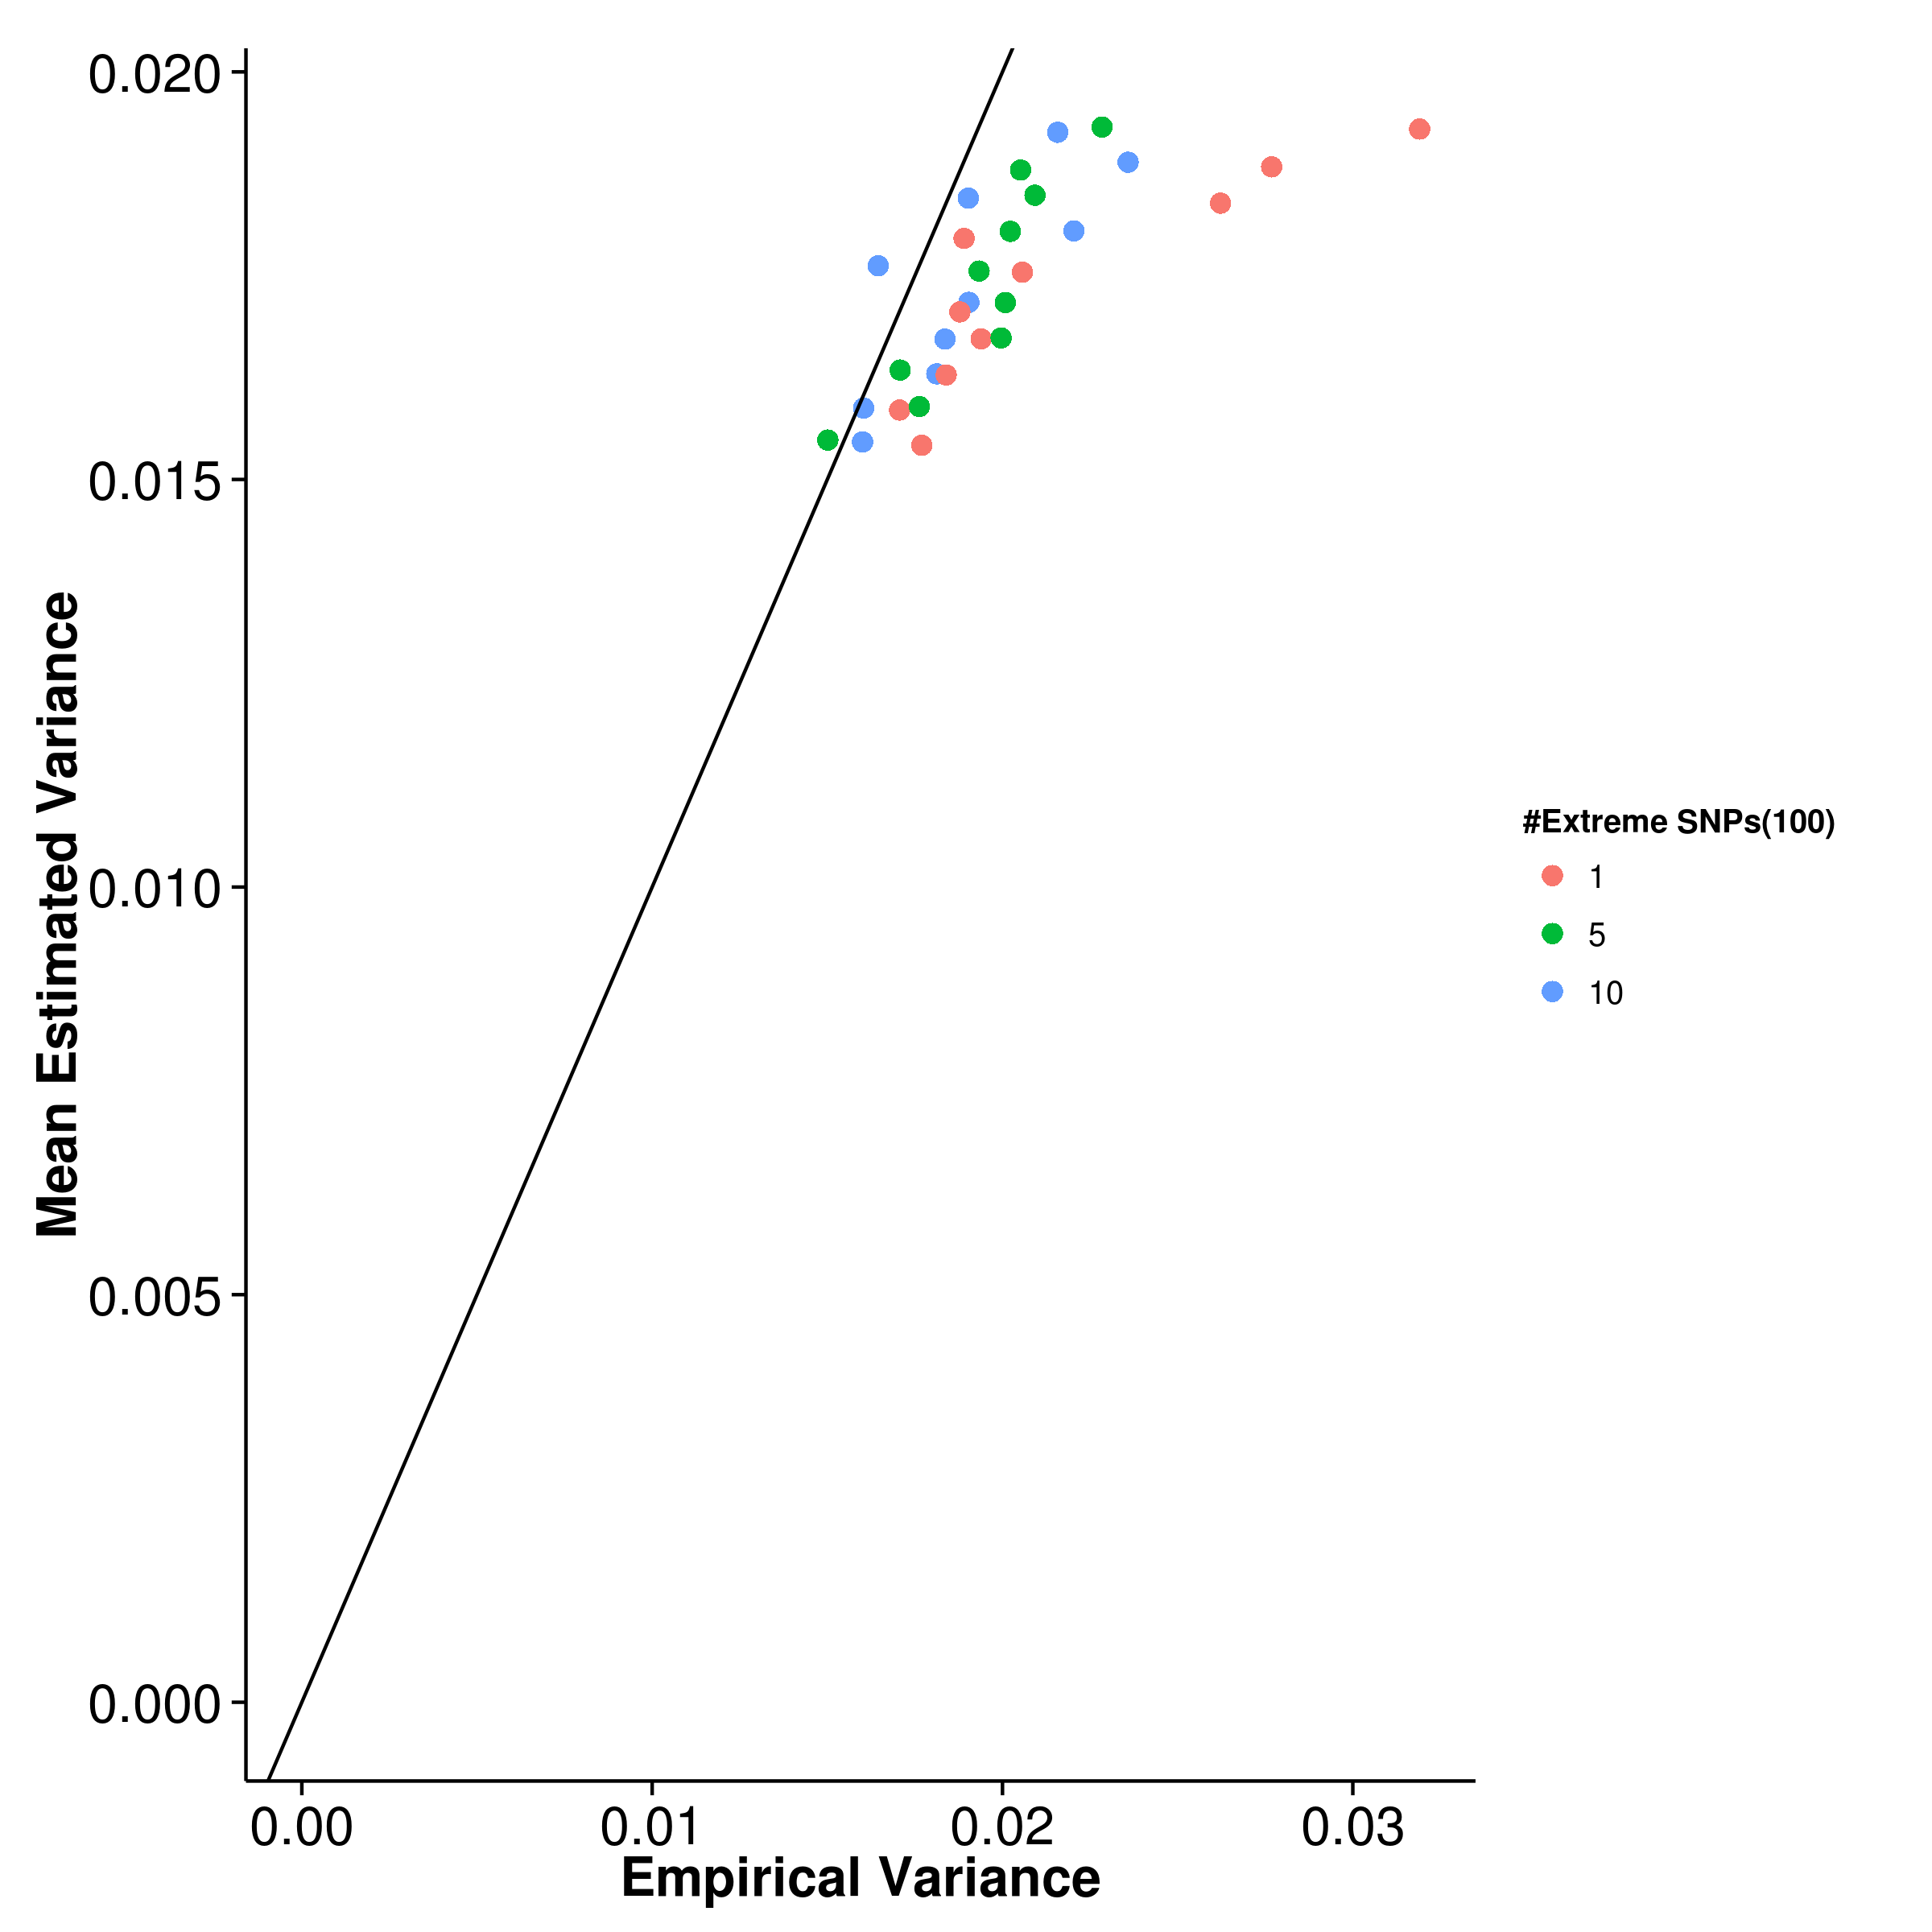
\includegraphics{figure/he_summary/extreme_100c/shrek_QtE_Rand_sdCom.png}}
				\label{fig:shrekQtEx100cVarCom}
			}
			\subfloat[GCTA]{
				\scalebox{.4}{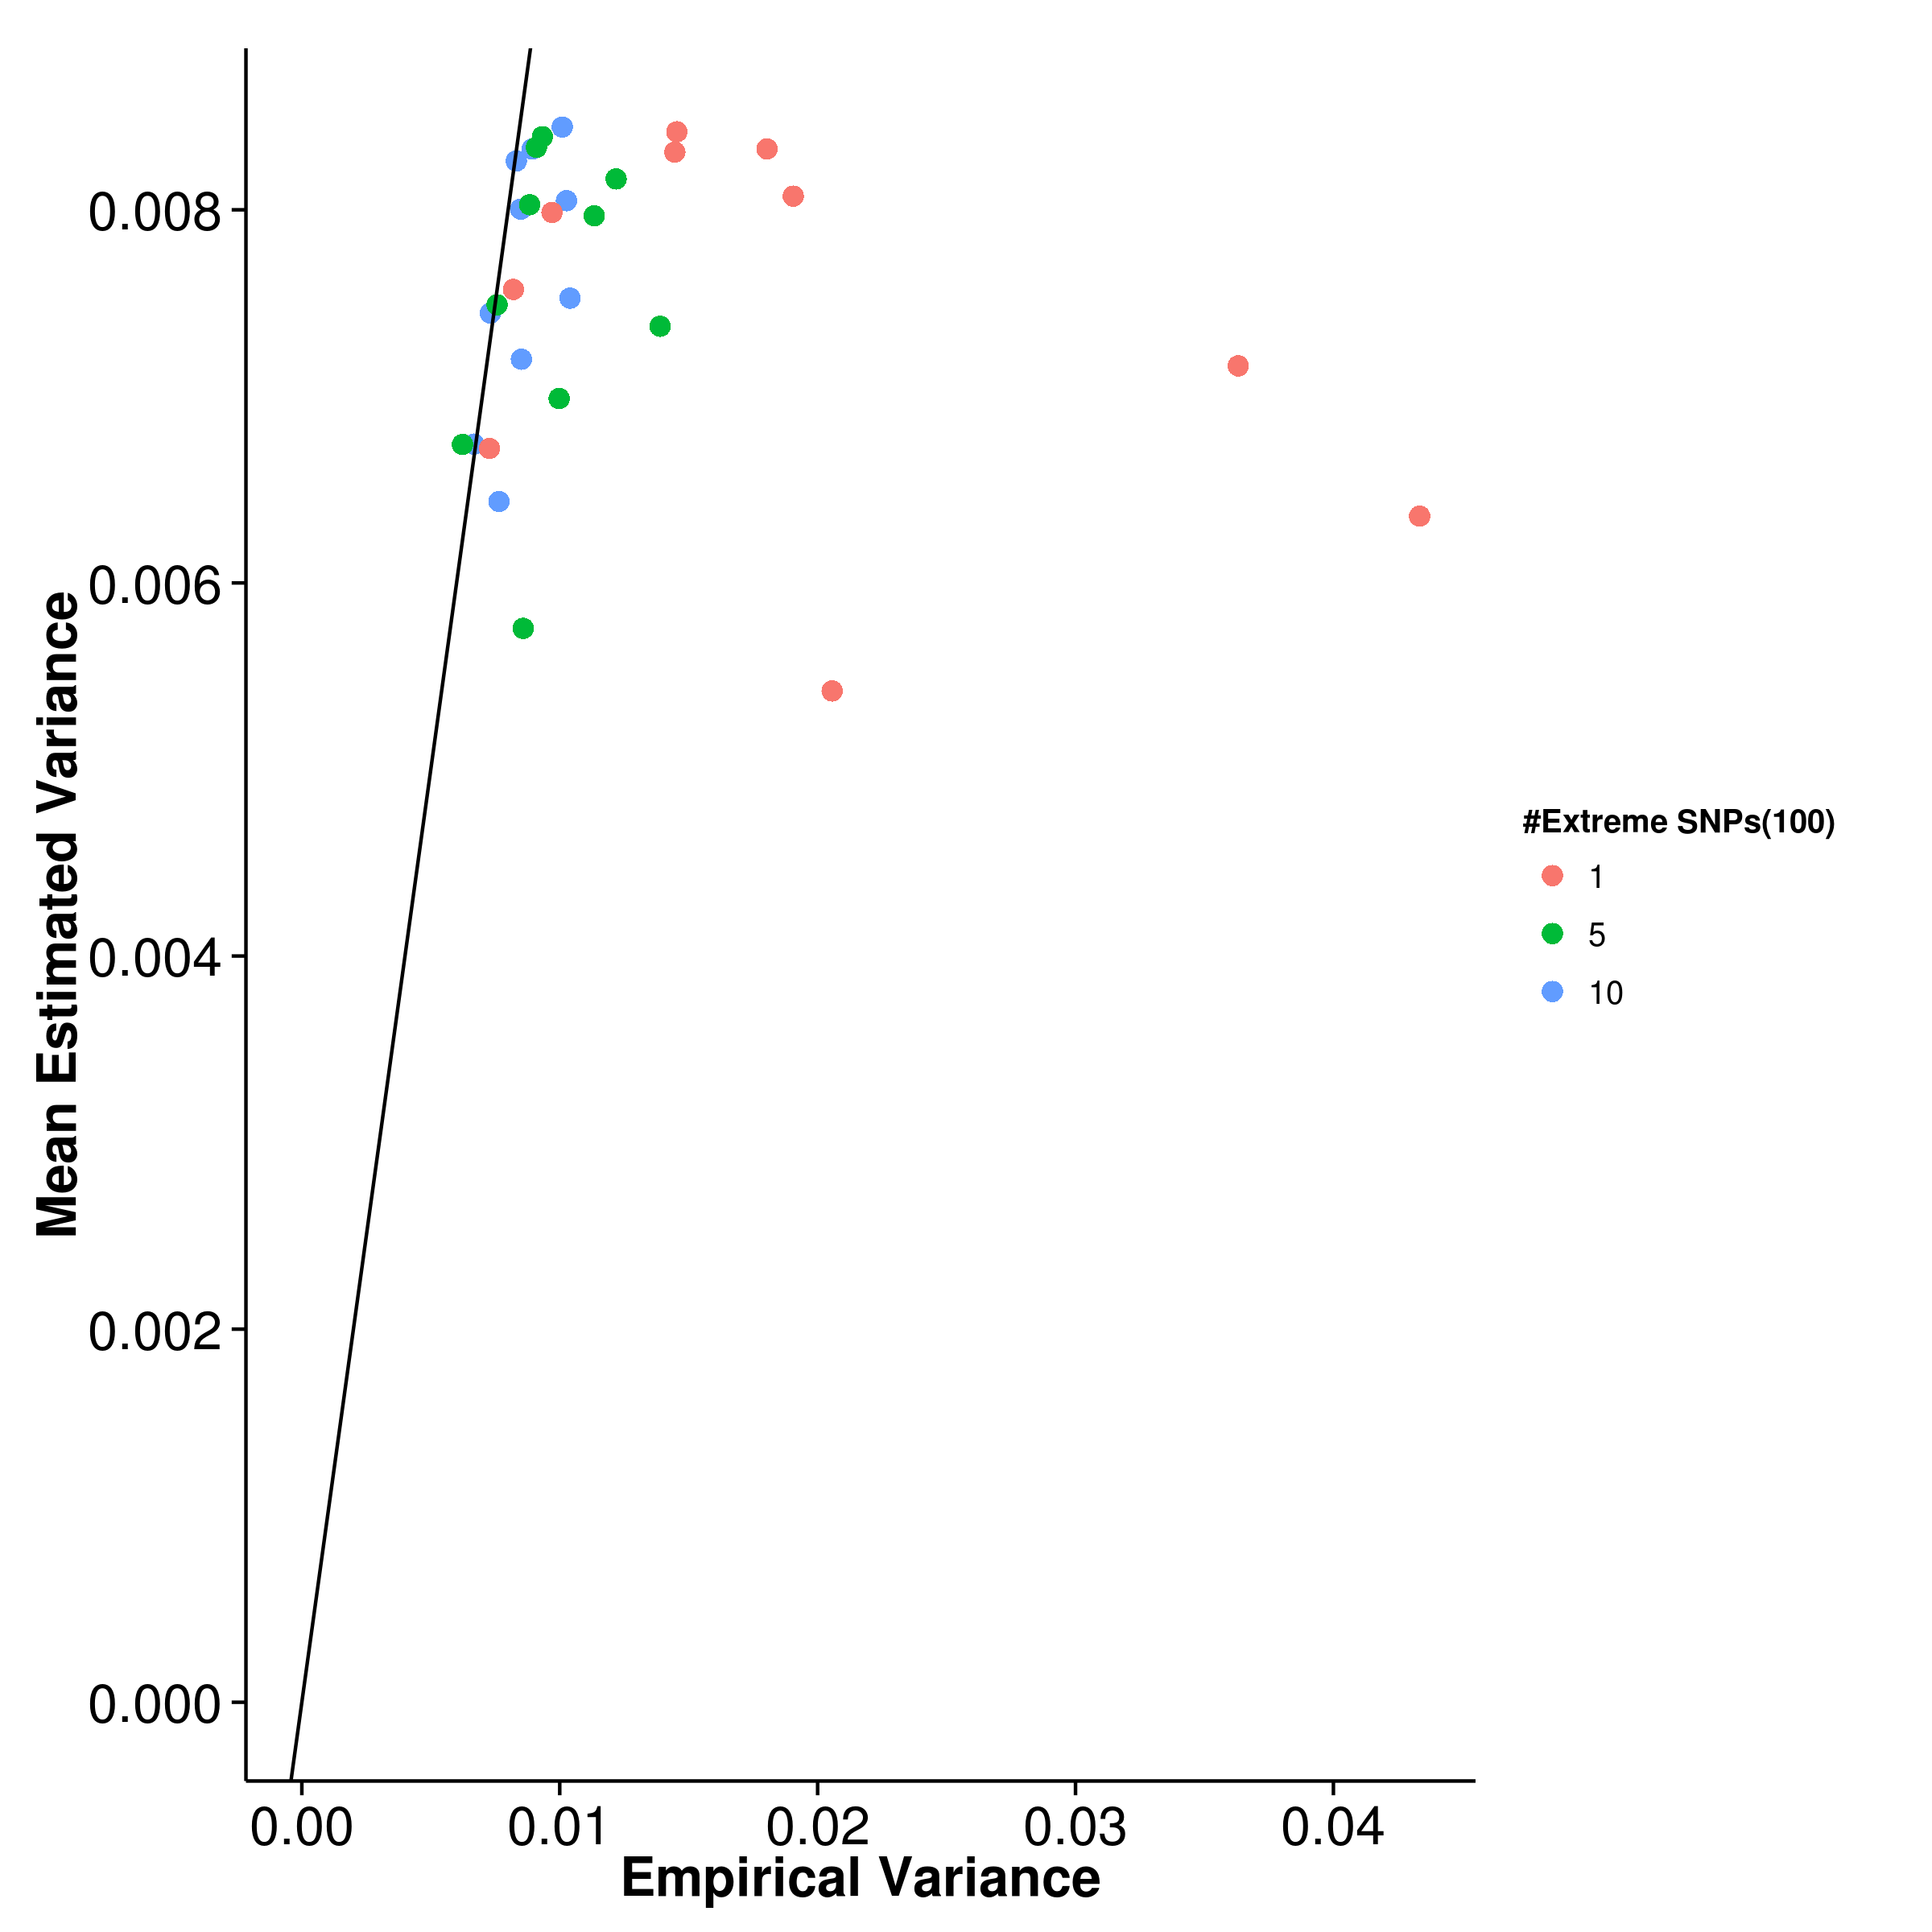
\includegraphics{figure/he_summary/extreme_100c/gcta_QtE_Rand_sdCom.png}}
				\label{fig:gctaQtEx100cVarCom}
			}\\
			\subfloat[LDSC with fix intercept]{
				\scalebox{.4}{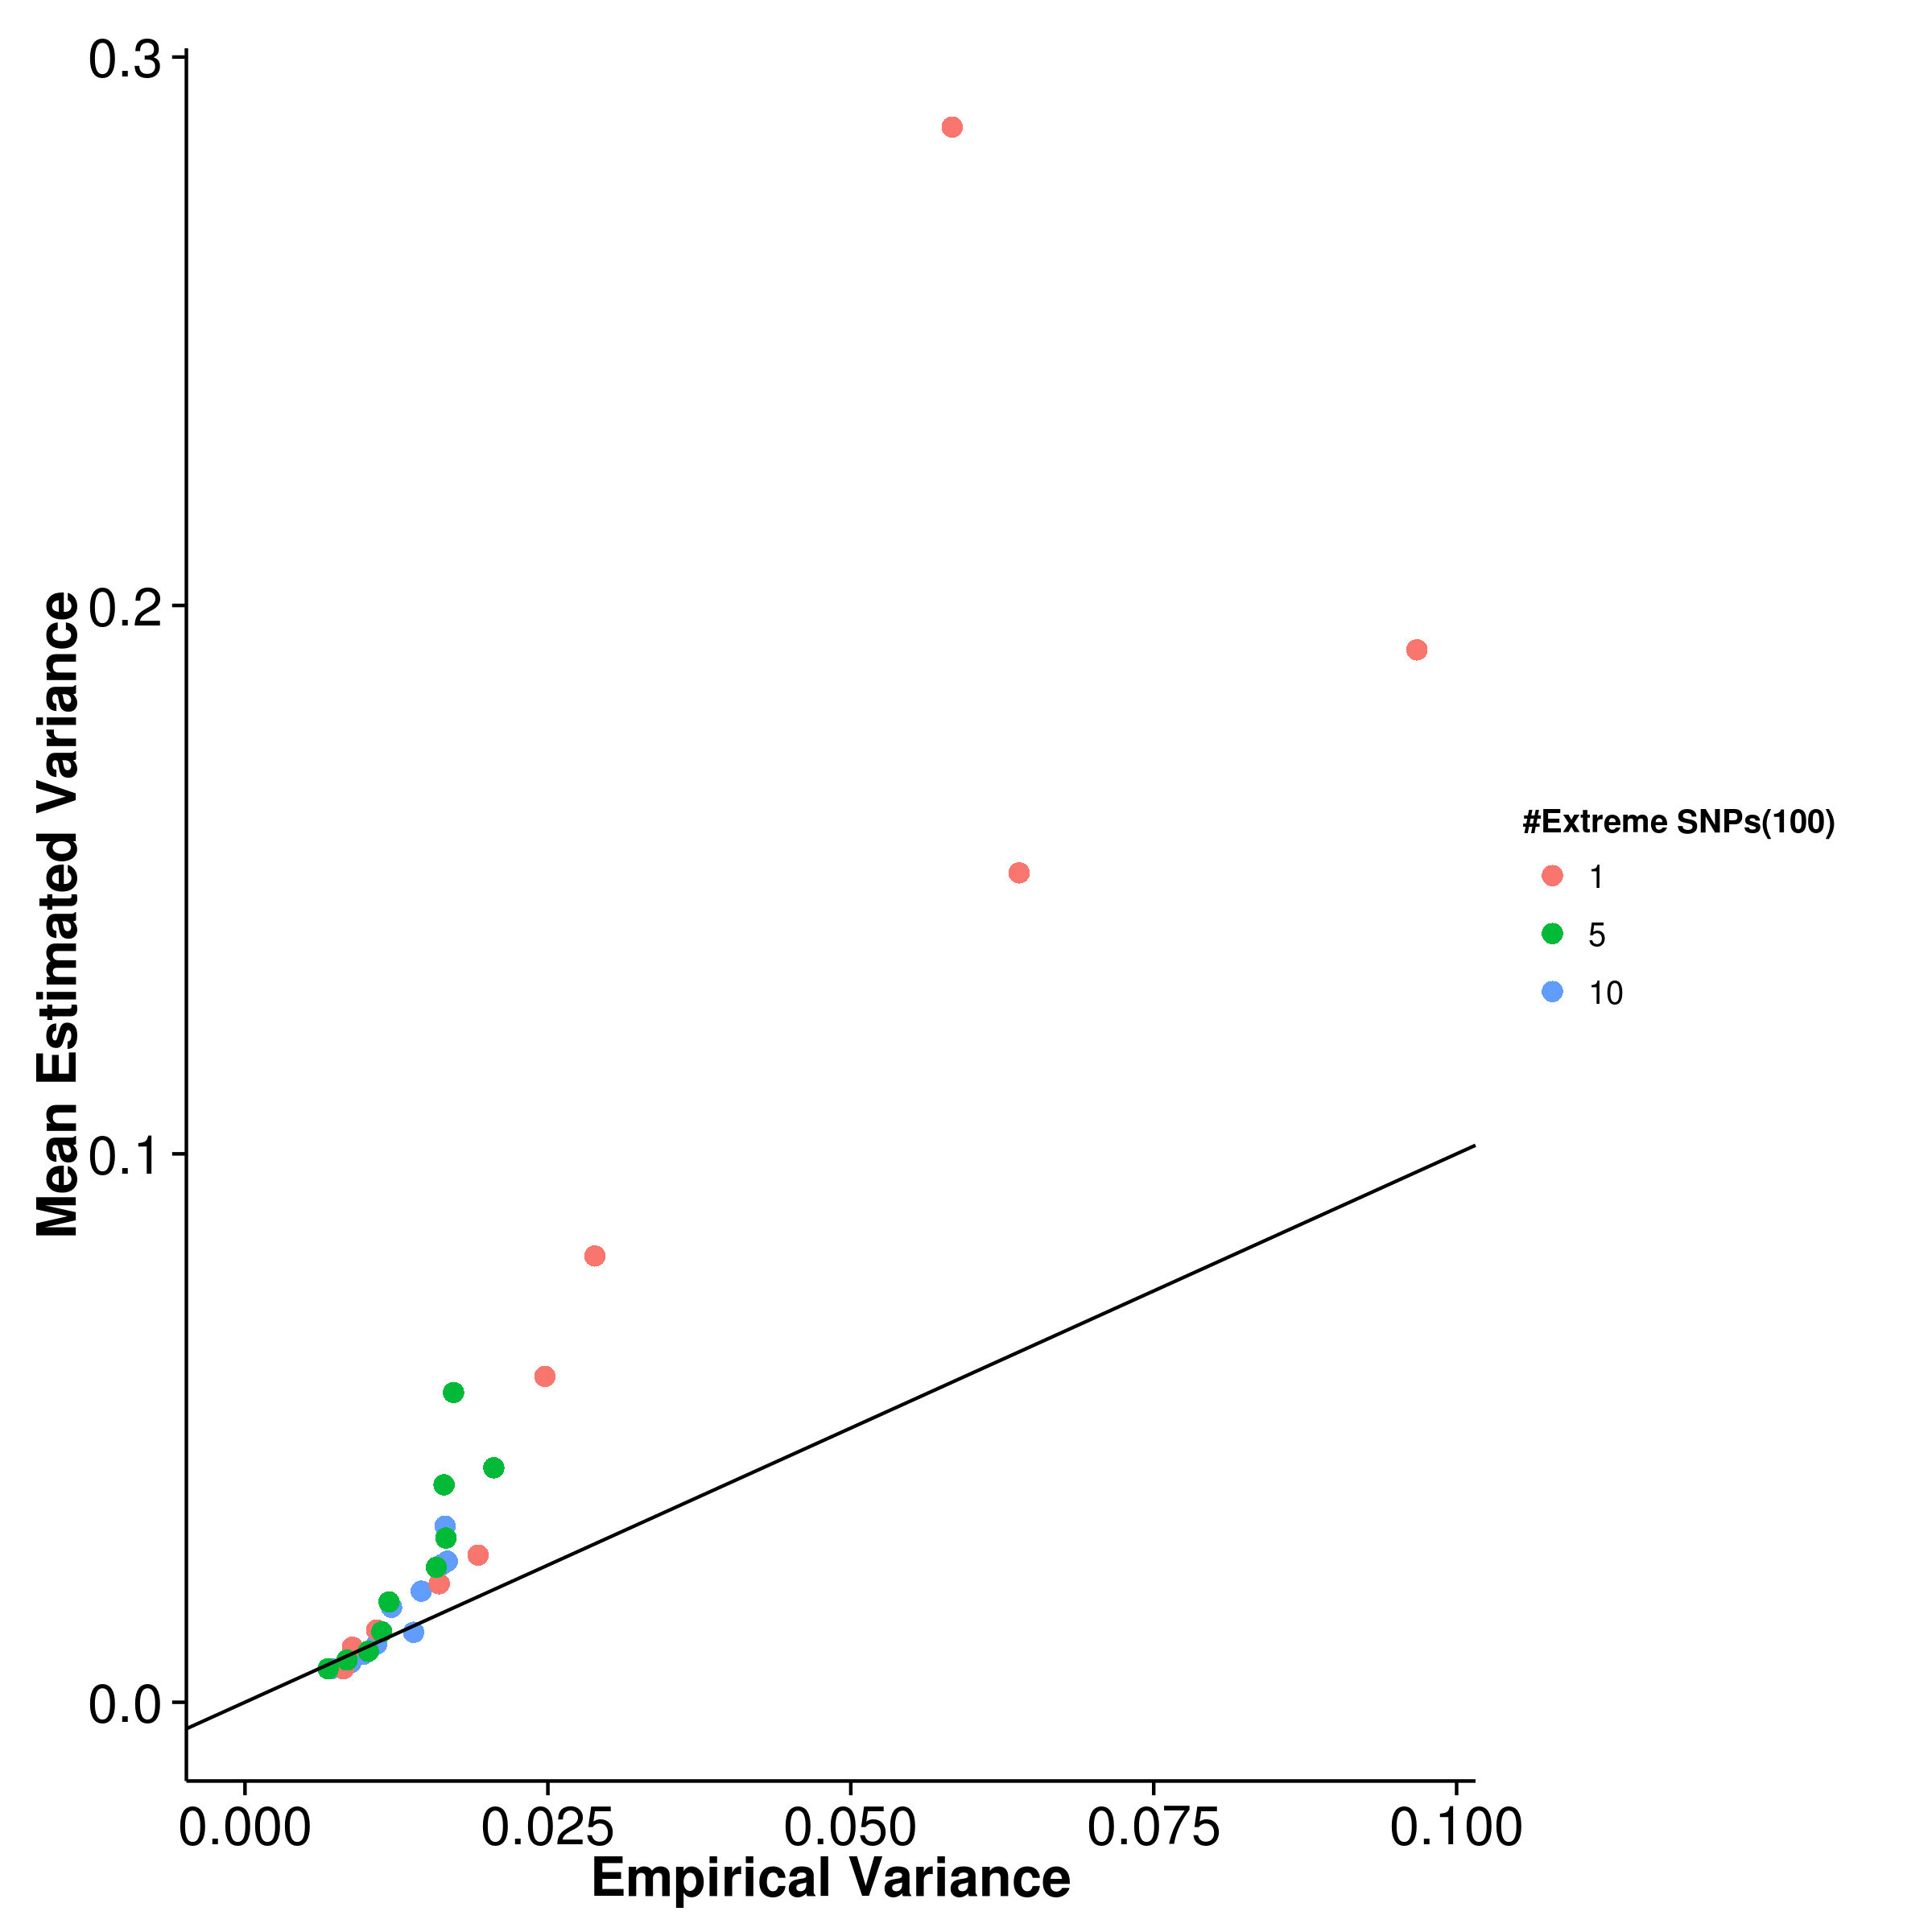
\includegraphics{figure/he_summary/extreme_100c/ldsc_QtE_Rand_sdCom.png}}
				\label{fig:ldscQtEx100cVarCom}
			}
			\subfloat[LDSC with intercept estimation]{
				
				\scalebox{.4}{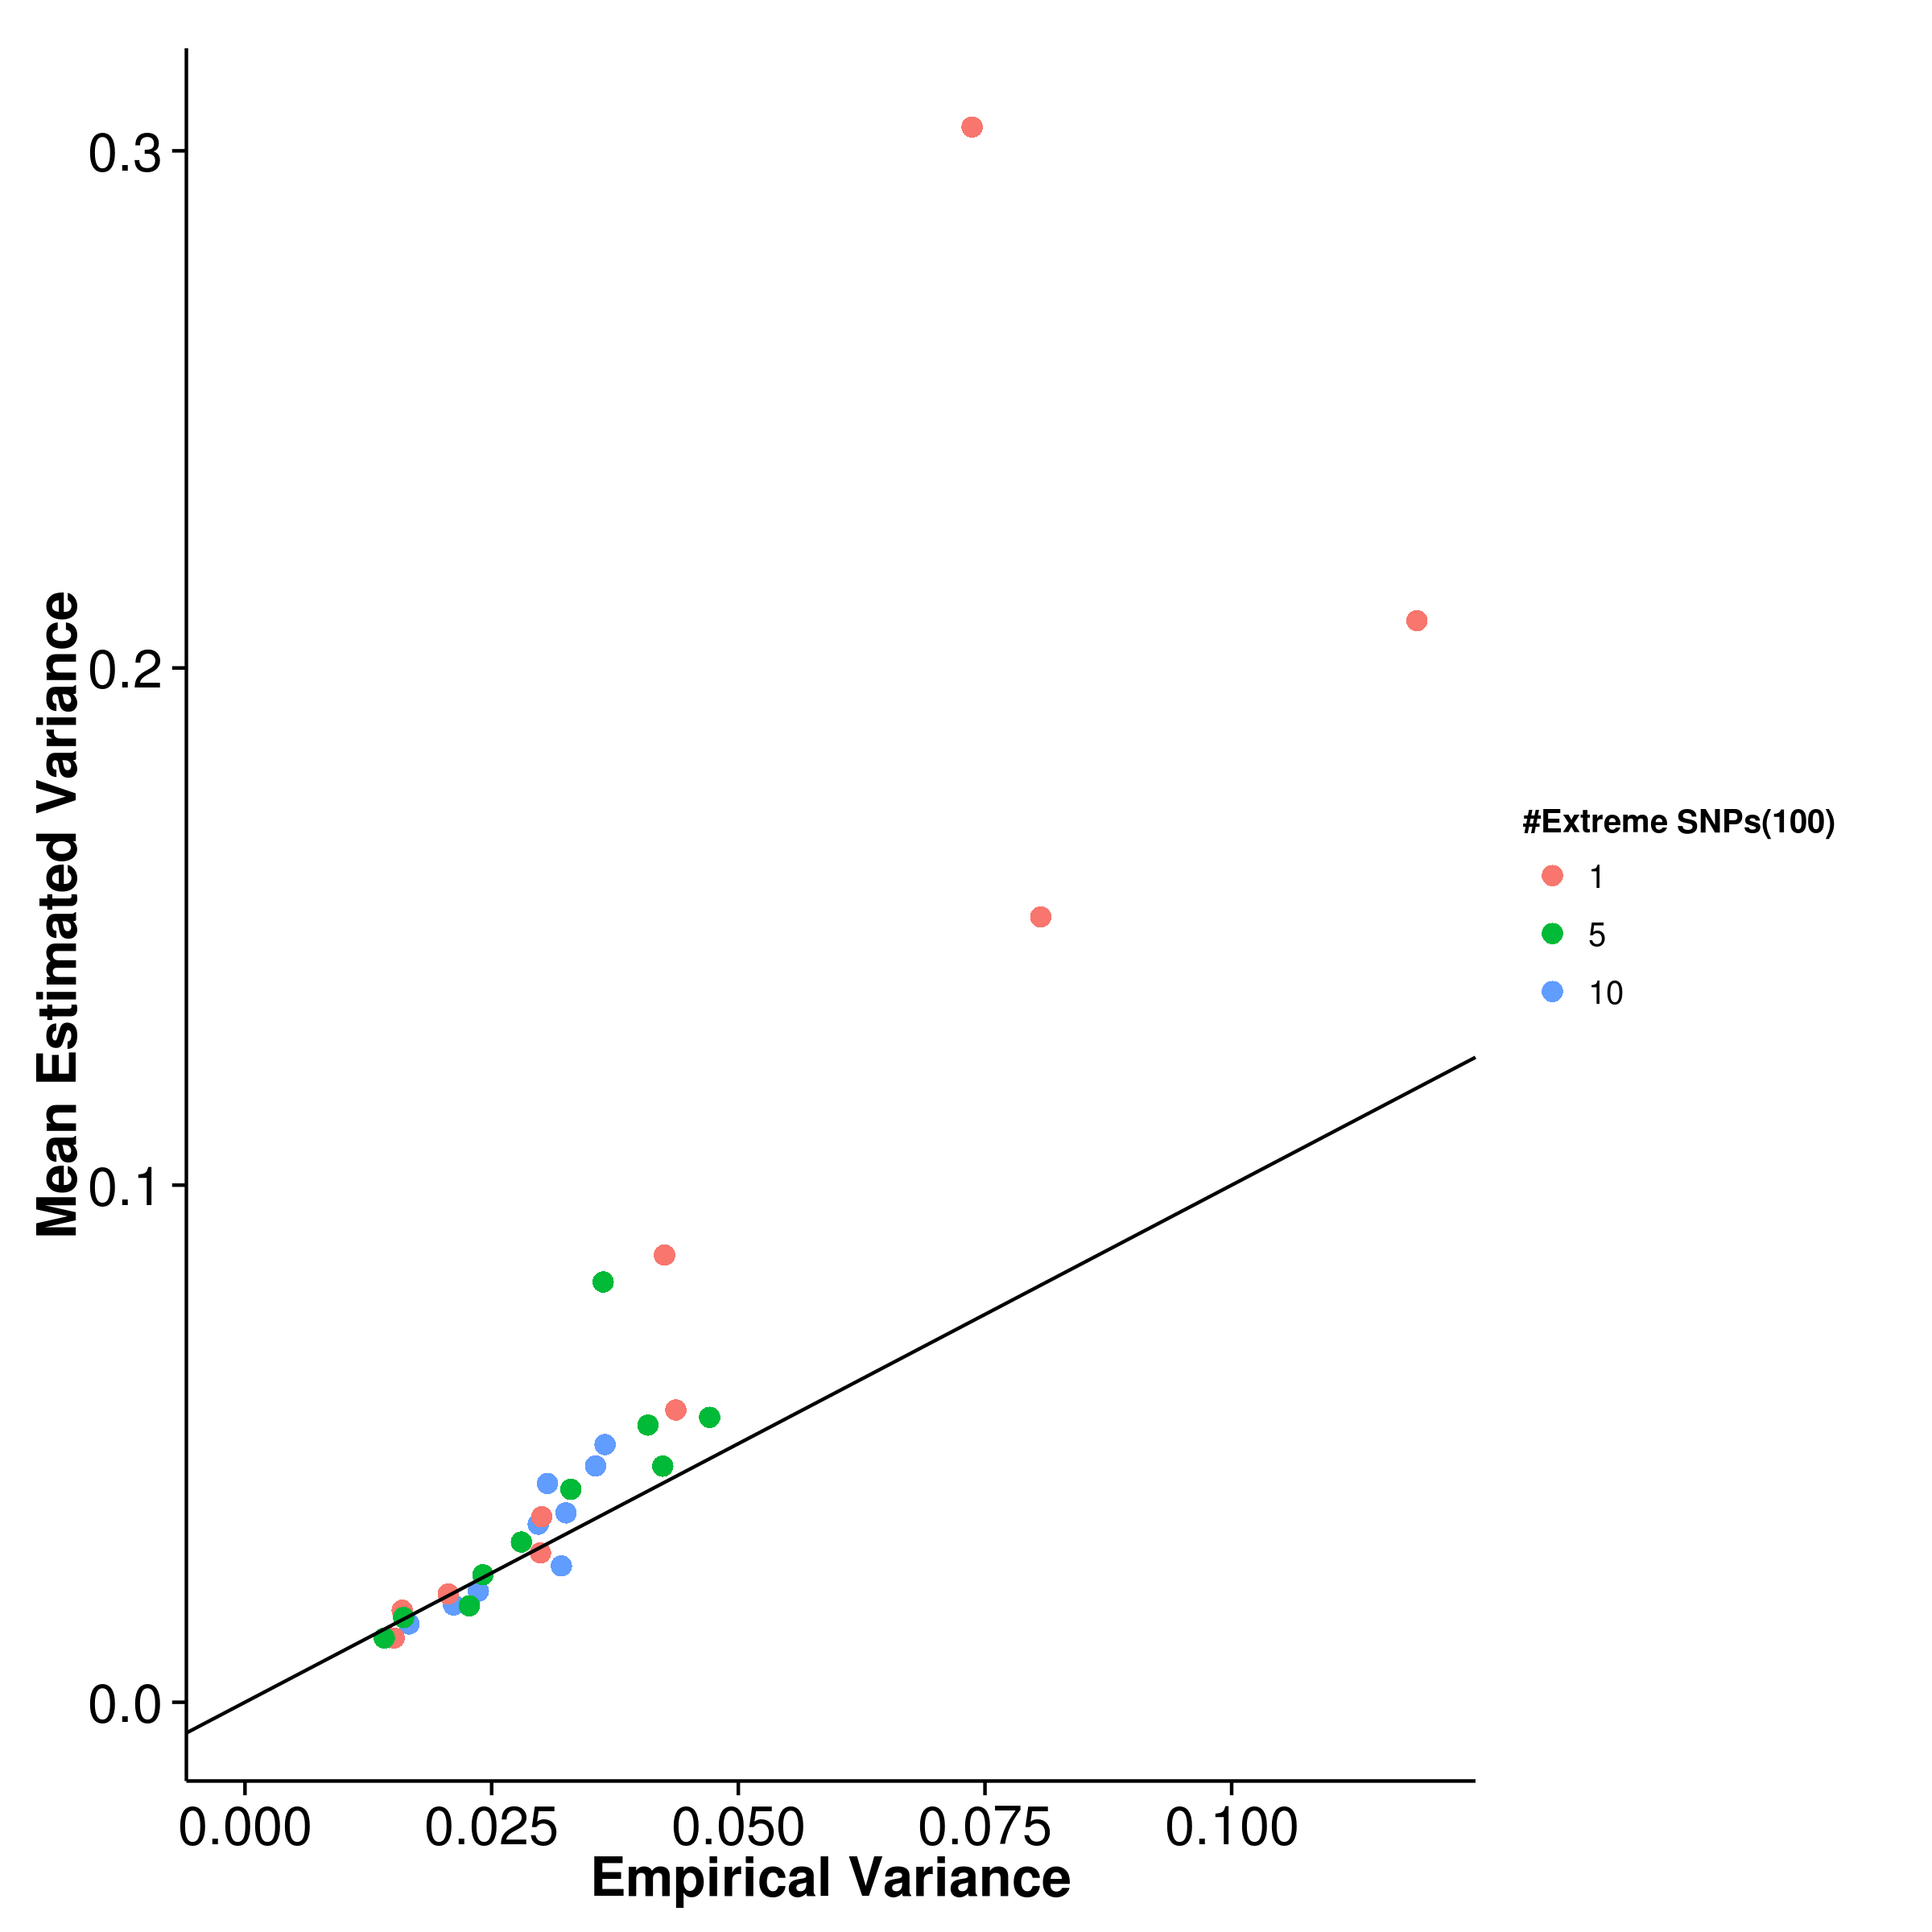
\includegraphics{figure/he_summary/extreme_100c/ldscIn_QtE_Rand_sdCom.png}}
				\label{fig:ldscInQtEx100cVarCom}
			}
			\caption[Estimation of Variance in Extreme Effect Size Simulation]
			{Estimated variance of results from quantitative trait simulation with extreme effect size simulation when compared to the empirical variance.
				100 causal \glspl{SNP} were simulated.
				\gls{shrek} and \gls{gcta} generally under-estimate the variance with the magnitude of bias being the highest when there is only 1 \gls{SNP} with extreme effect.
				On the other hand, \gls{ldsc} tends to over-estimate the variance and it can overestimate the variance by more than 3 folds when there is only 1 \gls{SNP} with extreme effect.
			} 
			\label{fig:QtEx100cVarCom}
		\end{figure}
		For some diseases such as Hirschsprung's disease, a small number of \glspl{SNP} can account for majority of the effect with a large number of \glspl{SNP} with small effect size. 
		Therefore we were interested to test the performance of heritability estimation in such scenario.
		We performaned the quantitative trait simulation with 100 causal \glspl{SNP} where 1,5 or 10 of those \gls{SNP}(s) has a large effect.
		
		When assessing the mean estimation of heritability (\cref{fig:QtEx100cMean}), the performance of the algorithms were similar to that in the quantitative trait simulation.
		The only exception was when 1 \gls{SNP} with large effect was simulated, the mean estimation of \gls{ldsc} and \gls{gcta} fluctuates (\cref{fig:gctaQtEx100cMean,fig:ldscQtEx100cMean,fig:ldscInQtEx100cMean}).
		The same fluctuation was not observed in \gls{shrek} (\cref{fig:shrekQtEx100cMean}). 
		Similarly, the empirical variance of the estimation (\cref{fig:QtEx100cVar}) from \gls{gcta} and \gls{ldsc} increases and fluctuates when only 1 \gls{SNP} with large effect was simulated.
		It was most obvious in the case of \gls{ldsc} where the variance increased drastically as the heritability is high (\cref{fig:ldscQtEx100cVar}).
		However, \gls{shrek} does not seems to be affected and were robust to the number of \glspl{SNP} with large effect. 
		
		The estimated variance were also affected by the number of \glspl{SNP} with large effect where the larges discrepancy between the estimated and empirical variance was observed when only 1 \gls{SNP} with large effect was simulated. 
		It was observed that both \gls{shrek} and \gls{gcta} tends to underestimates their empirical variance whereas \gls{ldsc} tends to overestimates the empirical variance. 
		The difference between the estimated and empirical variance for \gls{ldsc} with fixed effect can be as much as 3 fold. 
		
		To conclude, the performance of \gls{gcta} is superior to other algorithm(\cref{tab:mseEx100c}).
		However, if we only consider the algorithms using test statistic for heritability estimation, the performance of \gls{ldsc} is better than \gls{shrek} when there are more than 1 \gls{SNP} with large effect. 
		Again, as no confounding factors were simulated, \gls{ldsc} with fixed intercept outperforms \gls{ldsc} with intercept estimation.
		It was interesting to note that the \gls{mse} of \gls{shrek} was least affected by the number of \gls{SNP}(s) with large effect.
		   
		\begin{table}
			\centering
			\begin{tabular}{rrrrr}
				\toprule
				Number of Extreme SNPs&	SHREK&	LDSC&	LDSC-In&	GCTA \\
				\midrule
				1	&	0.0227	&	0.0393	&	0.0508	&	0.0206\\
				5	&	0.0203	&	0.0145	&	0.0316	&	0.00985\\
				10	&	0.0205	&	0.0129	&	0.0329	&	0.00939\\
				\bottomrule
			\end{tabular}
			\caption[MSE of Quantitative Trait Simulation with Extreme Effect Size]{
				\gls{mse} of quantitative trait simulation with extreme effect size.
				Of all the algorithms, \gls{gcta} has the lowest \gls{mse} in all situations.
				When comparing the performance of \gls{shrek} and \gls{ldsc}, \gls{shrek} only has a better performance when there is one \gls{SNP} with large effect. 
				For other scenarios, \gls{ldsc} with fixed intercept has better performance.
				However, we can observe that the performance of \gls{shrek} is very consistent and robust to the change in number of \glspl{SNP} with extreme effect size.
				}
			\label{tab:mseEx100c}
		\end{table}
		
		% CC Rand Effect
		\subsubsection{Case Control Simulation}
			\begin{figure}
			\centering
			\subfloat[SHREK]{
				\scalebox{.4}{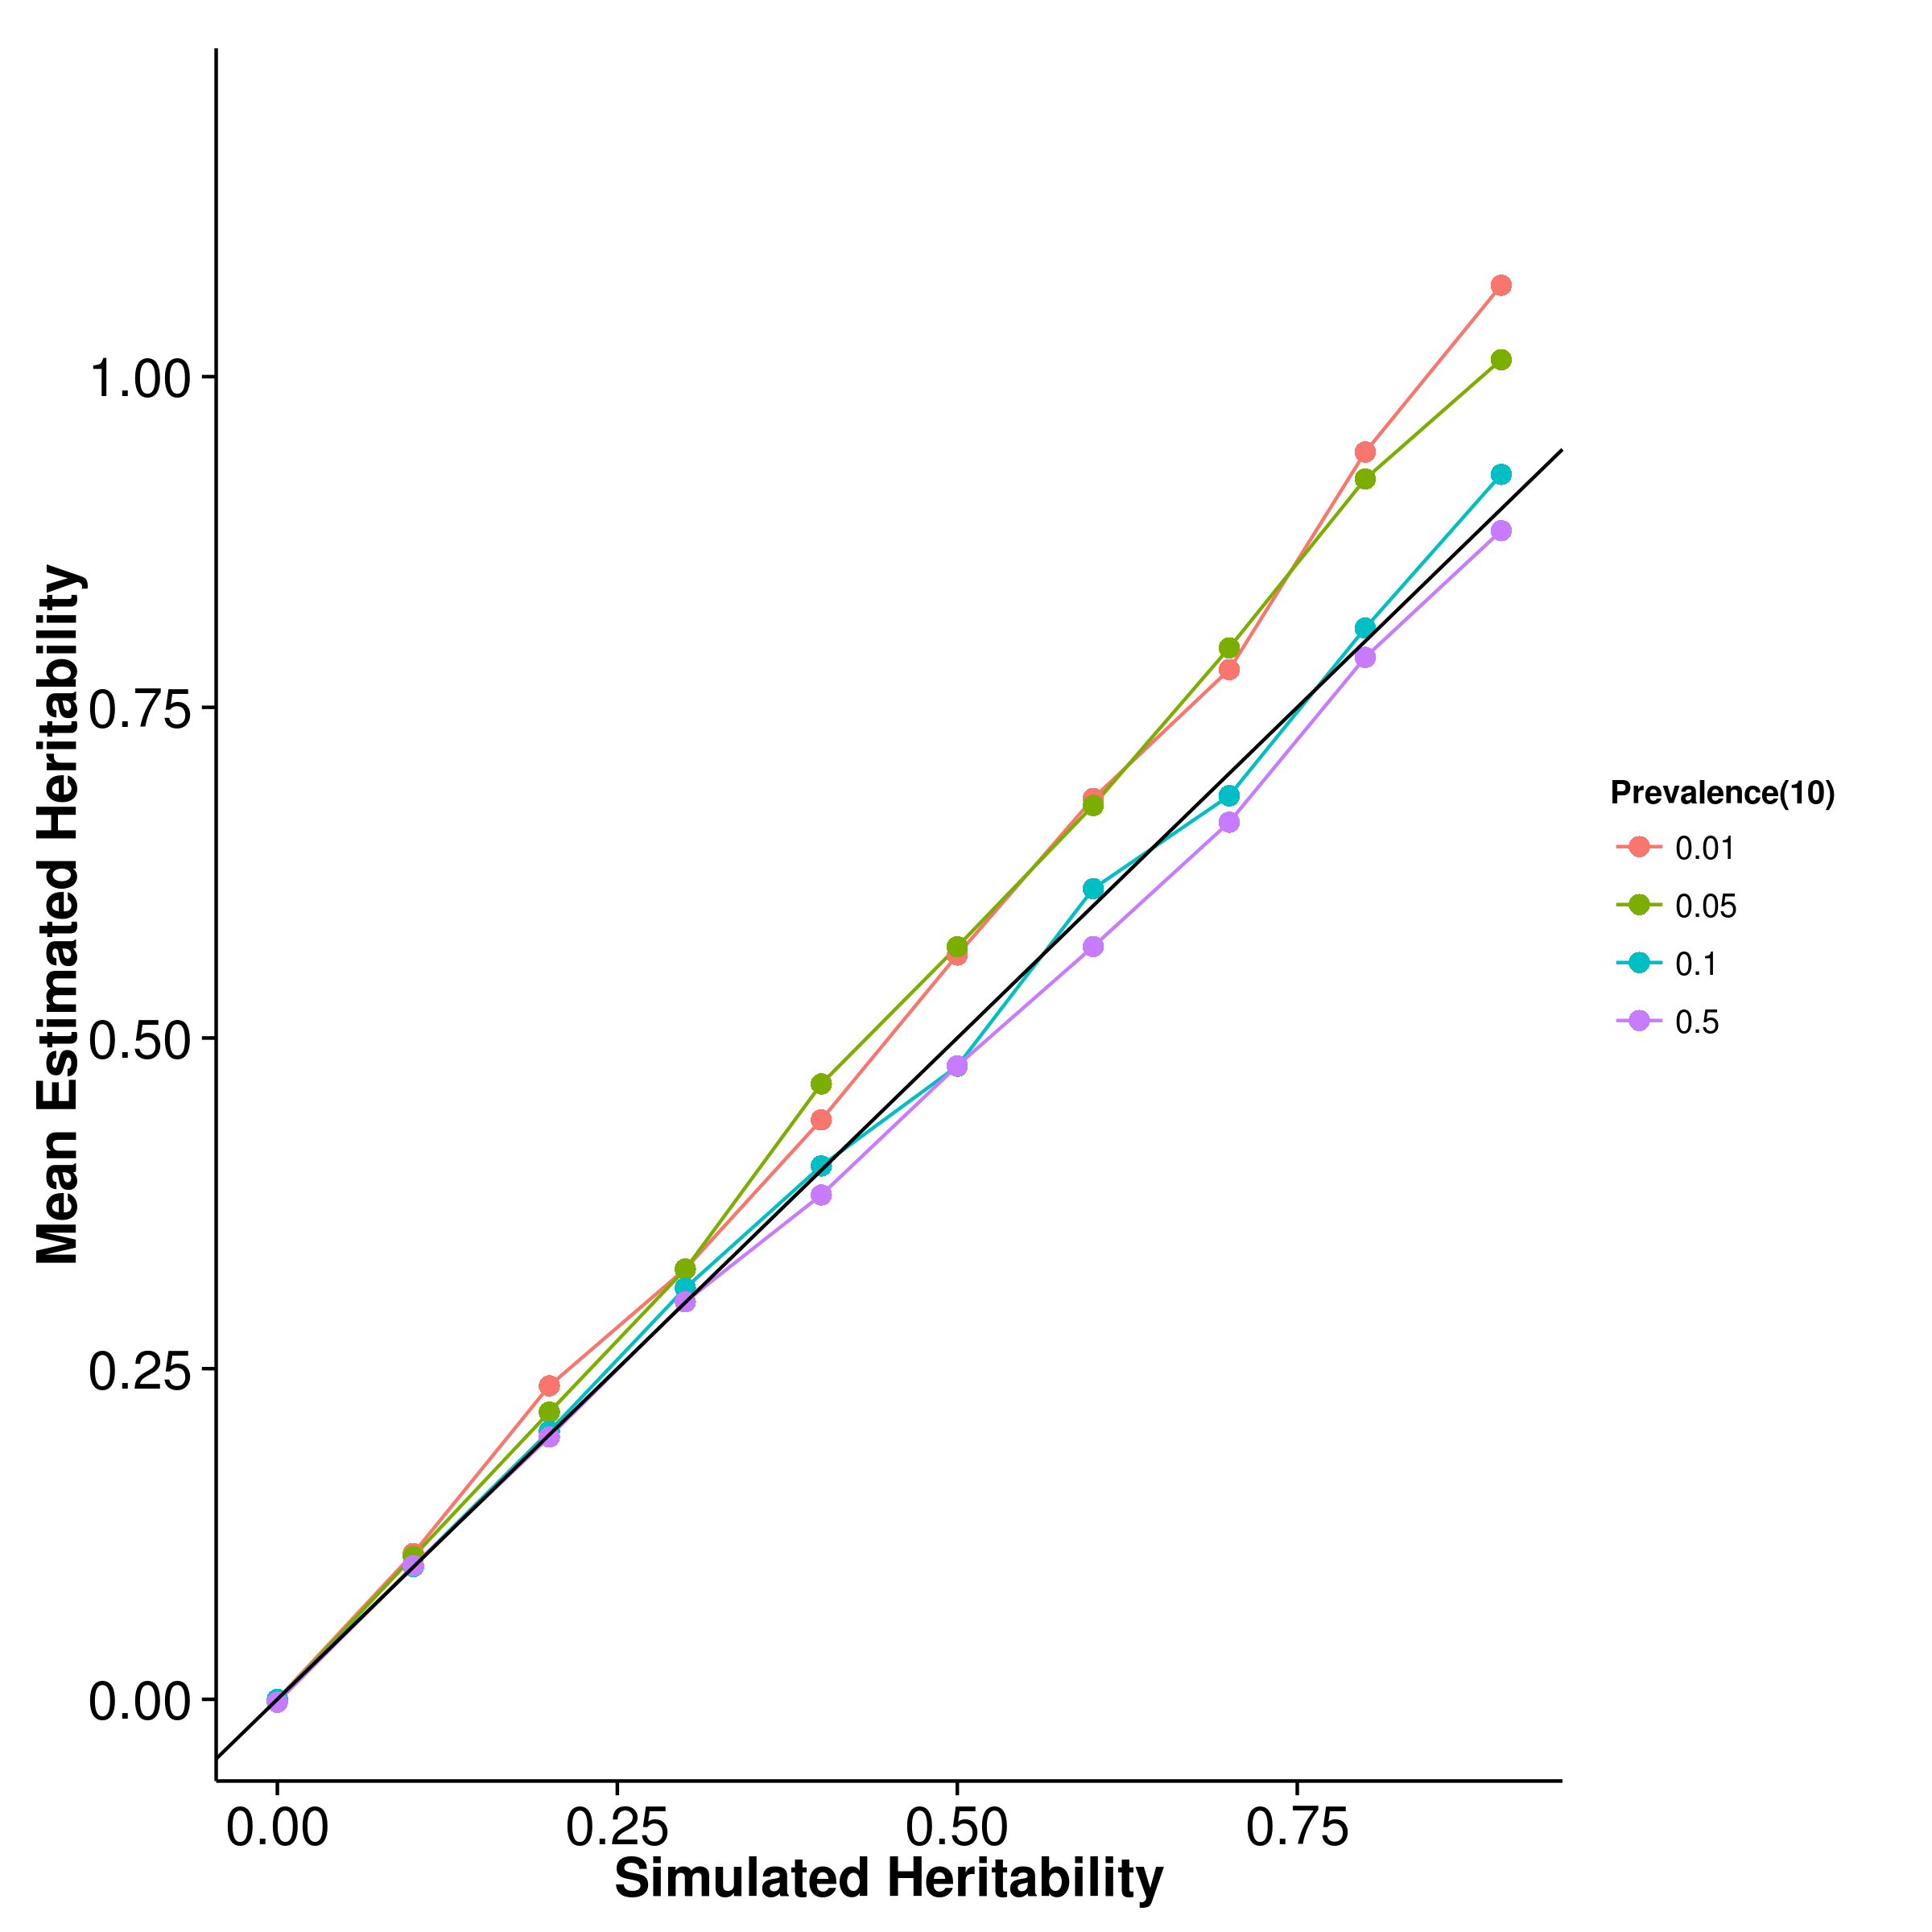
\includegraphics{figure/he_summary/cc_10c/shrek_CC_Rand_mean.png}}
				\label{fig:shrekCC10RandMean}
			}
			\subfloat[GCTA]{
				\scalebox{.4}{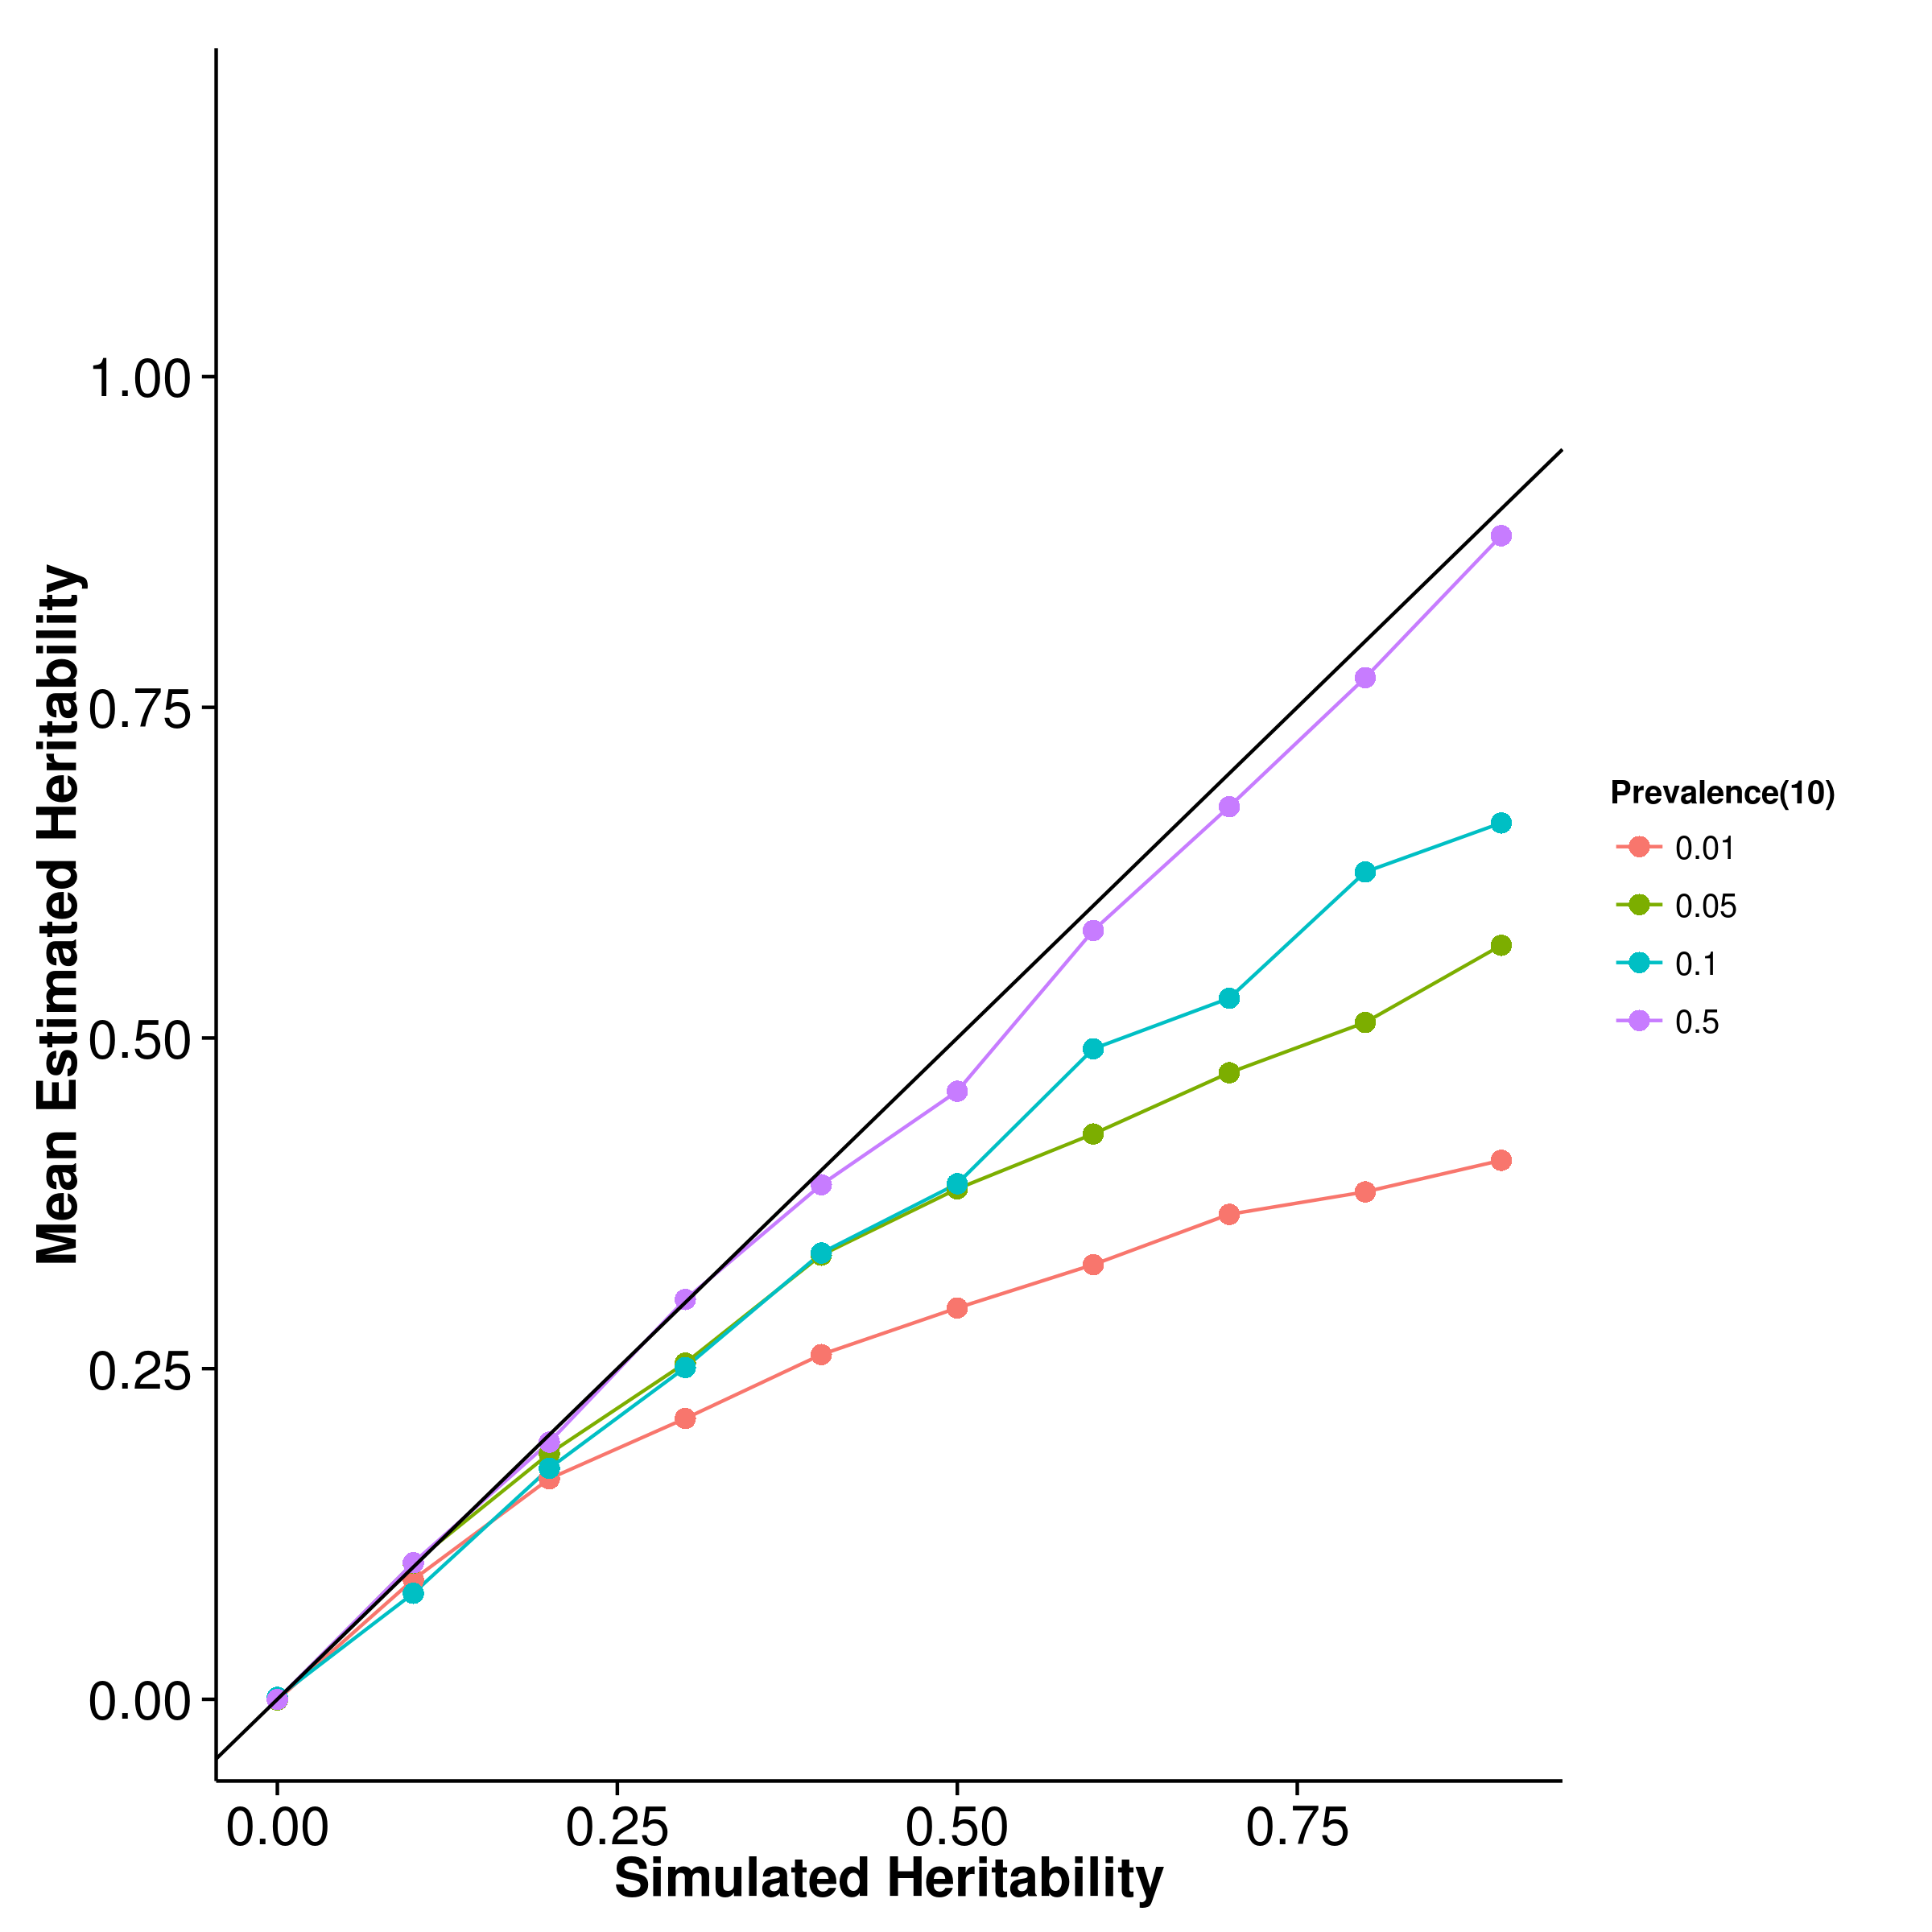
\includegraphics{figure/he_summary/cc_10c/gcta_CC_Rand_mean.png}}
				\label{fig:gctaCC10RandMean}
			}\\
			\subfloat[LDSC with fix intercept]{
				\scalebox{.4}{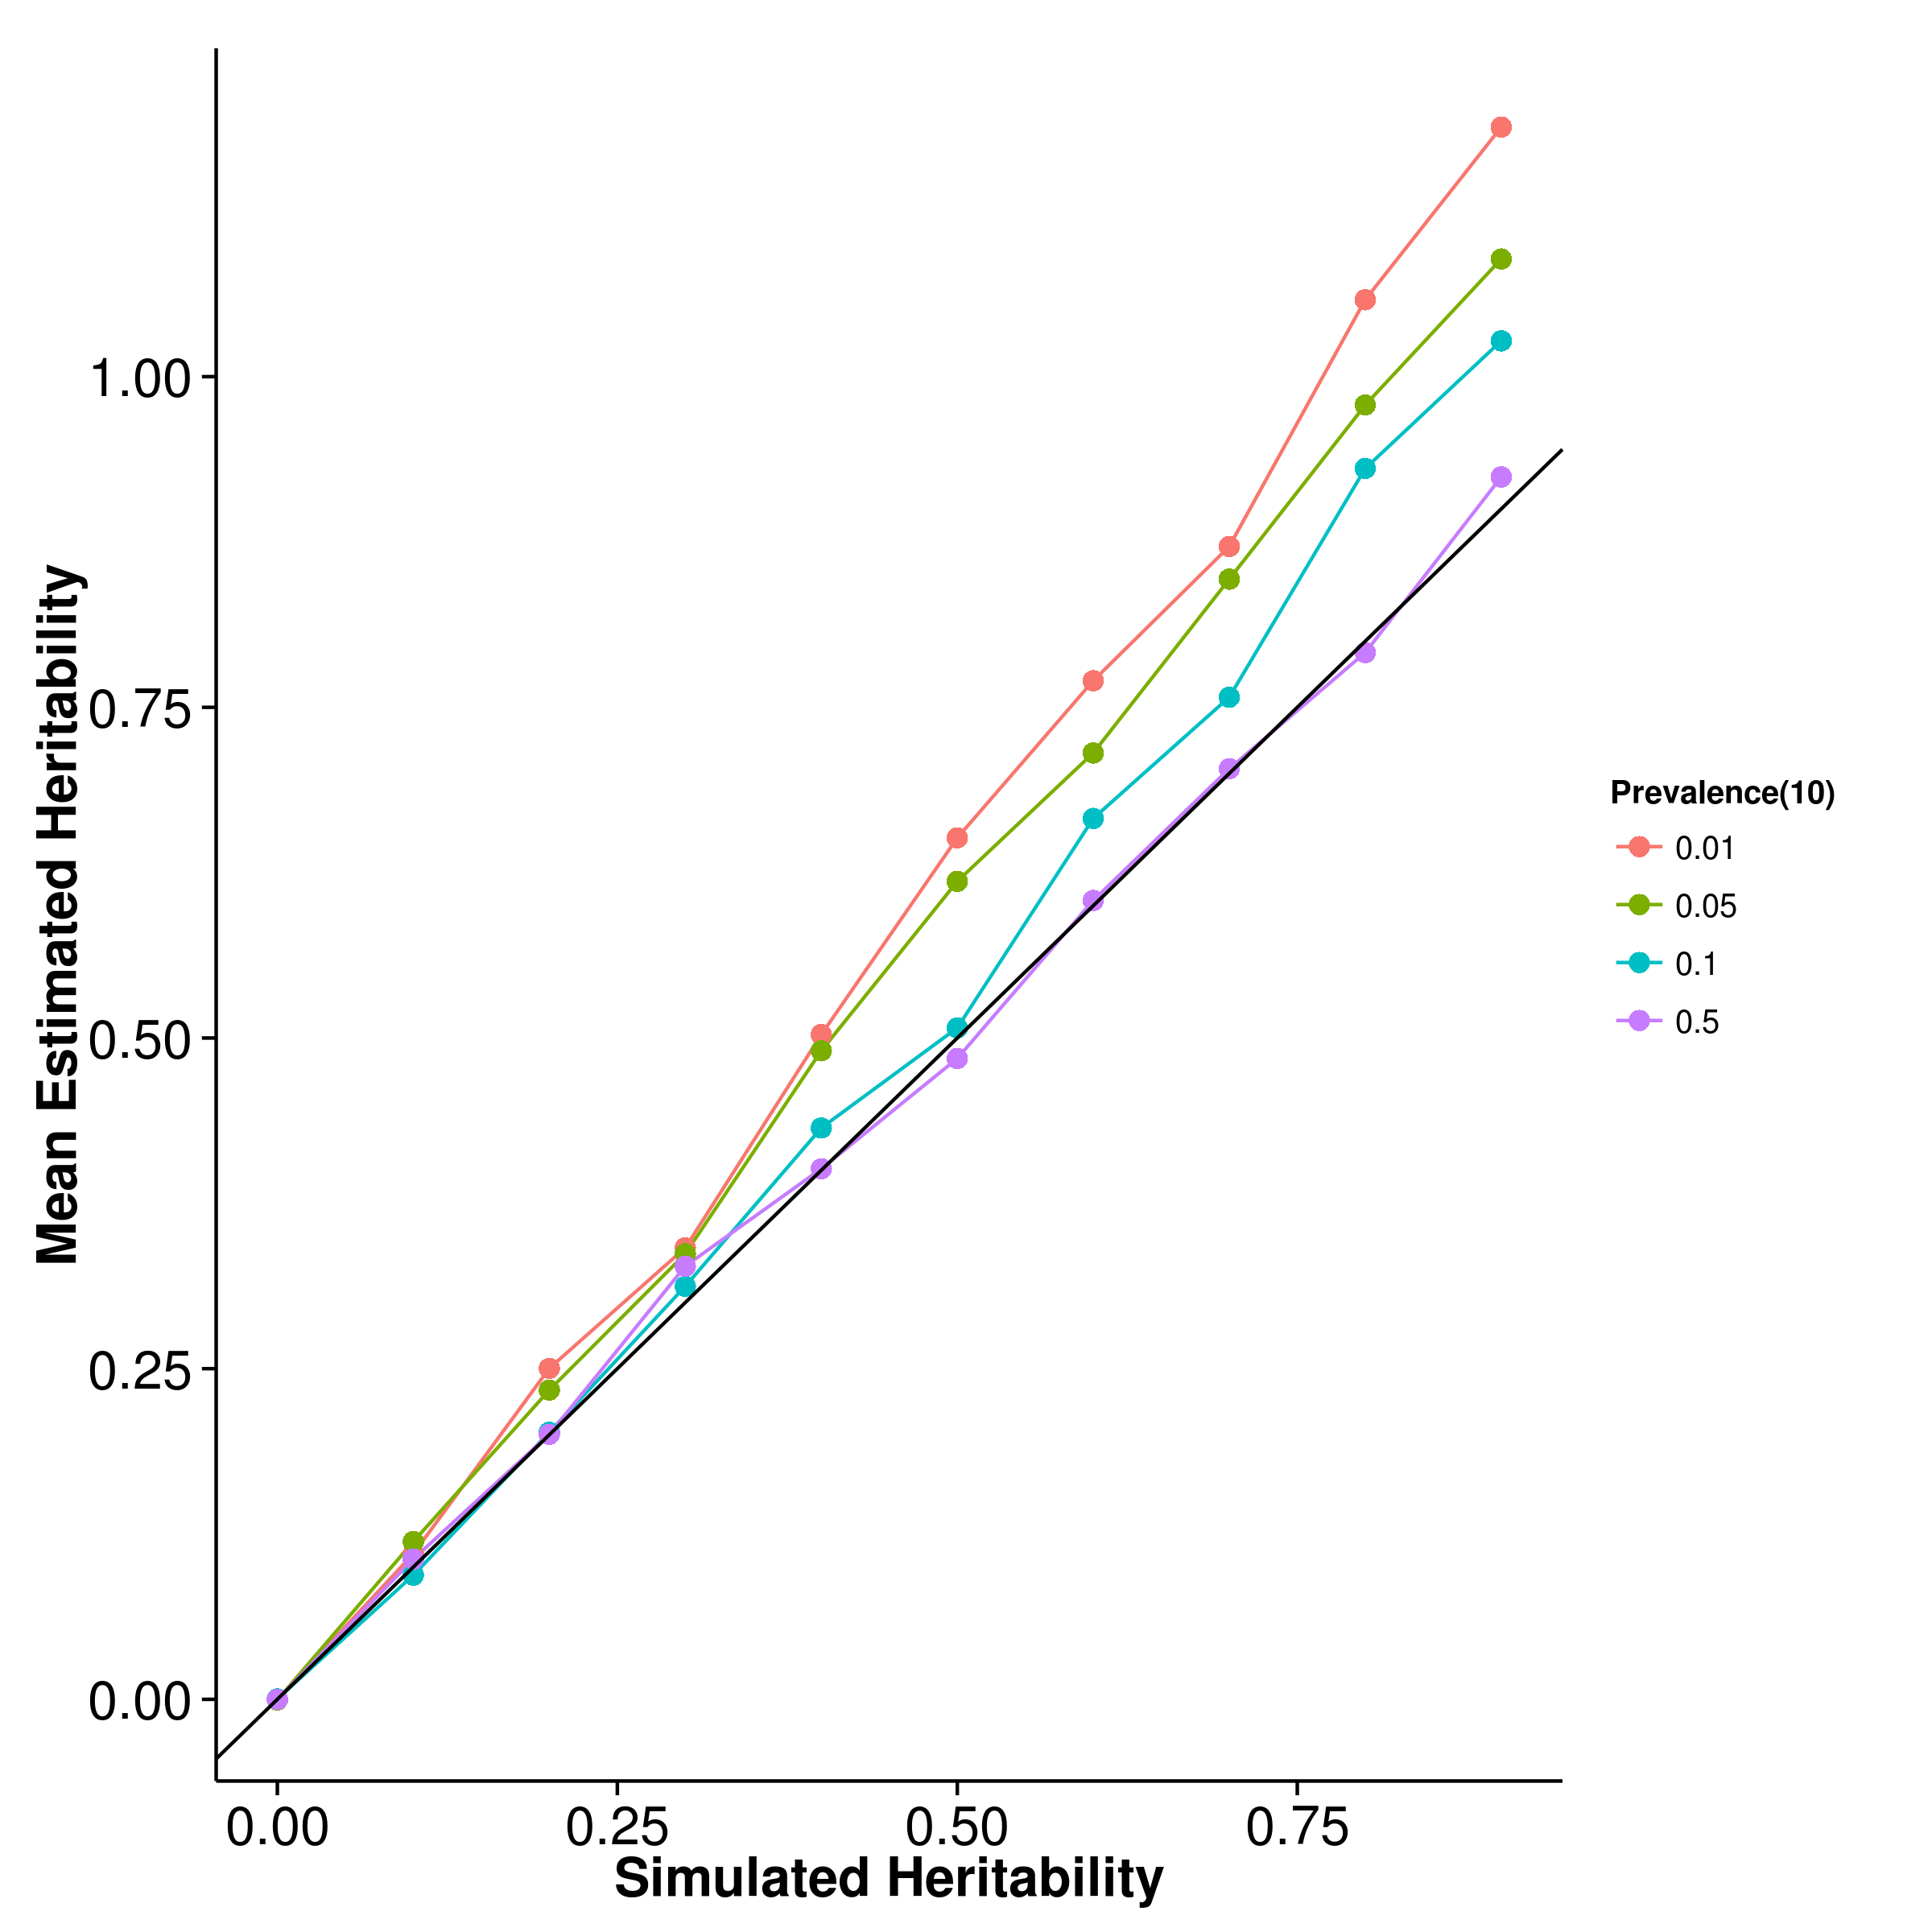
\includegraphics{figure/he_summary/cc_10c/ldsc_CC_Rand_mean.png}}
				\label{fig:ldscCC10RandMean}
			}
			\subfloat[LDSC with intercept estimation]{
				
				\scalebox{.4}{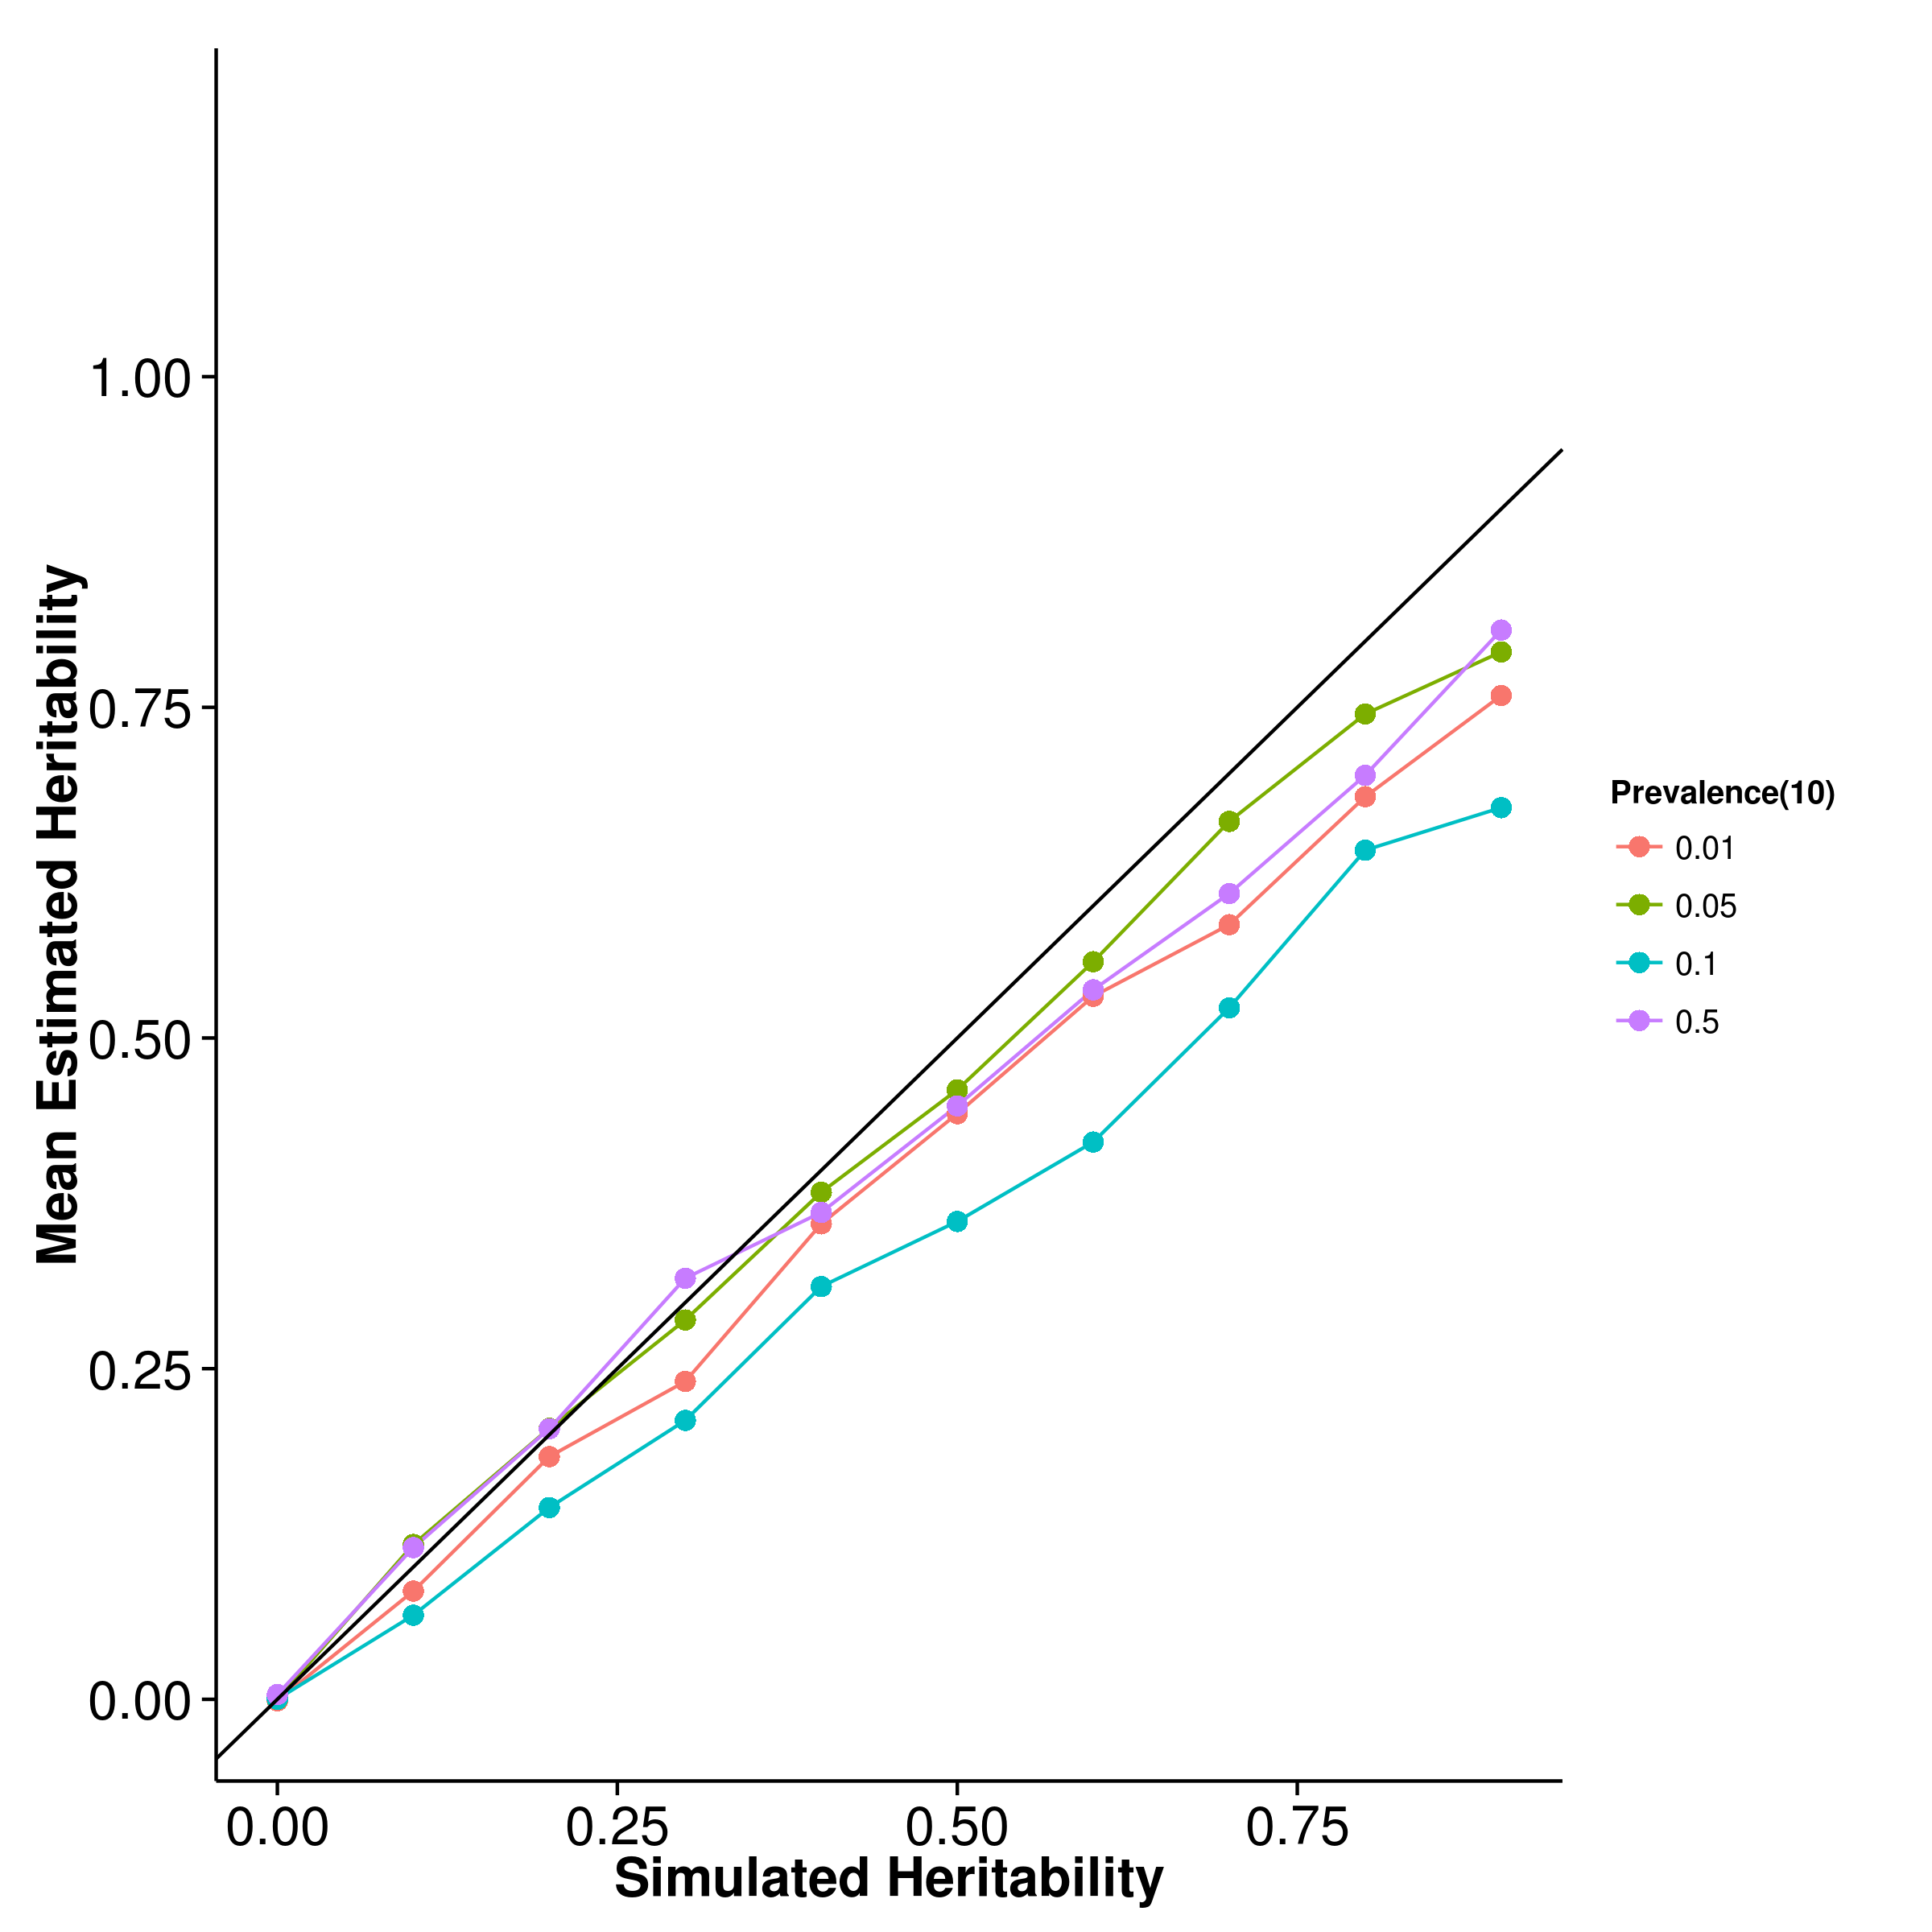
\includegraphics{figure/he_summary/cc_10c/ldscIn_CC_Rand_mean.png}}
				\label{fig:ldscInCC10RandMean}
			}
			\caption[Mean of Case Control Simulation Results (10 Causal)]
			{Mean of results from case control simulation with random effect size simulation with 10 causal \glspl{SNP}.
				The performance of \gls{gcta} was as suggested by \citet{Golan2014} where there was an underestimation as prevalence decreases.
				On the other hand, the upward bias of both \gls{ldsc} with fixed intercept and \gls{shrek} increases as the prevalence decreases whereas \gls{ldsc} with intercept estimation seems relatively robust to the change in prevalence.
				} 
			\label{fig:CC10RandMean}
		\end{figure}
		
		\begin{figure}
			\centering
			\subfloat[SHREK]{
				\scalebox{.4}{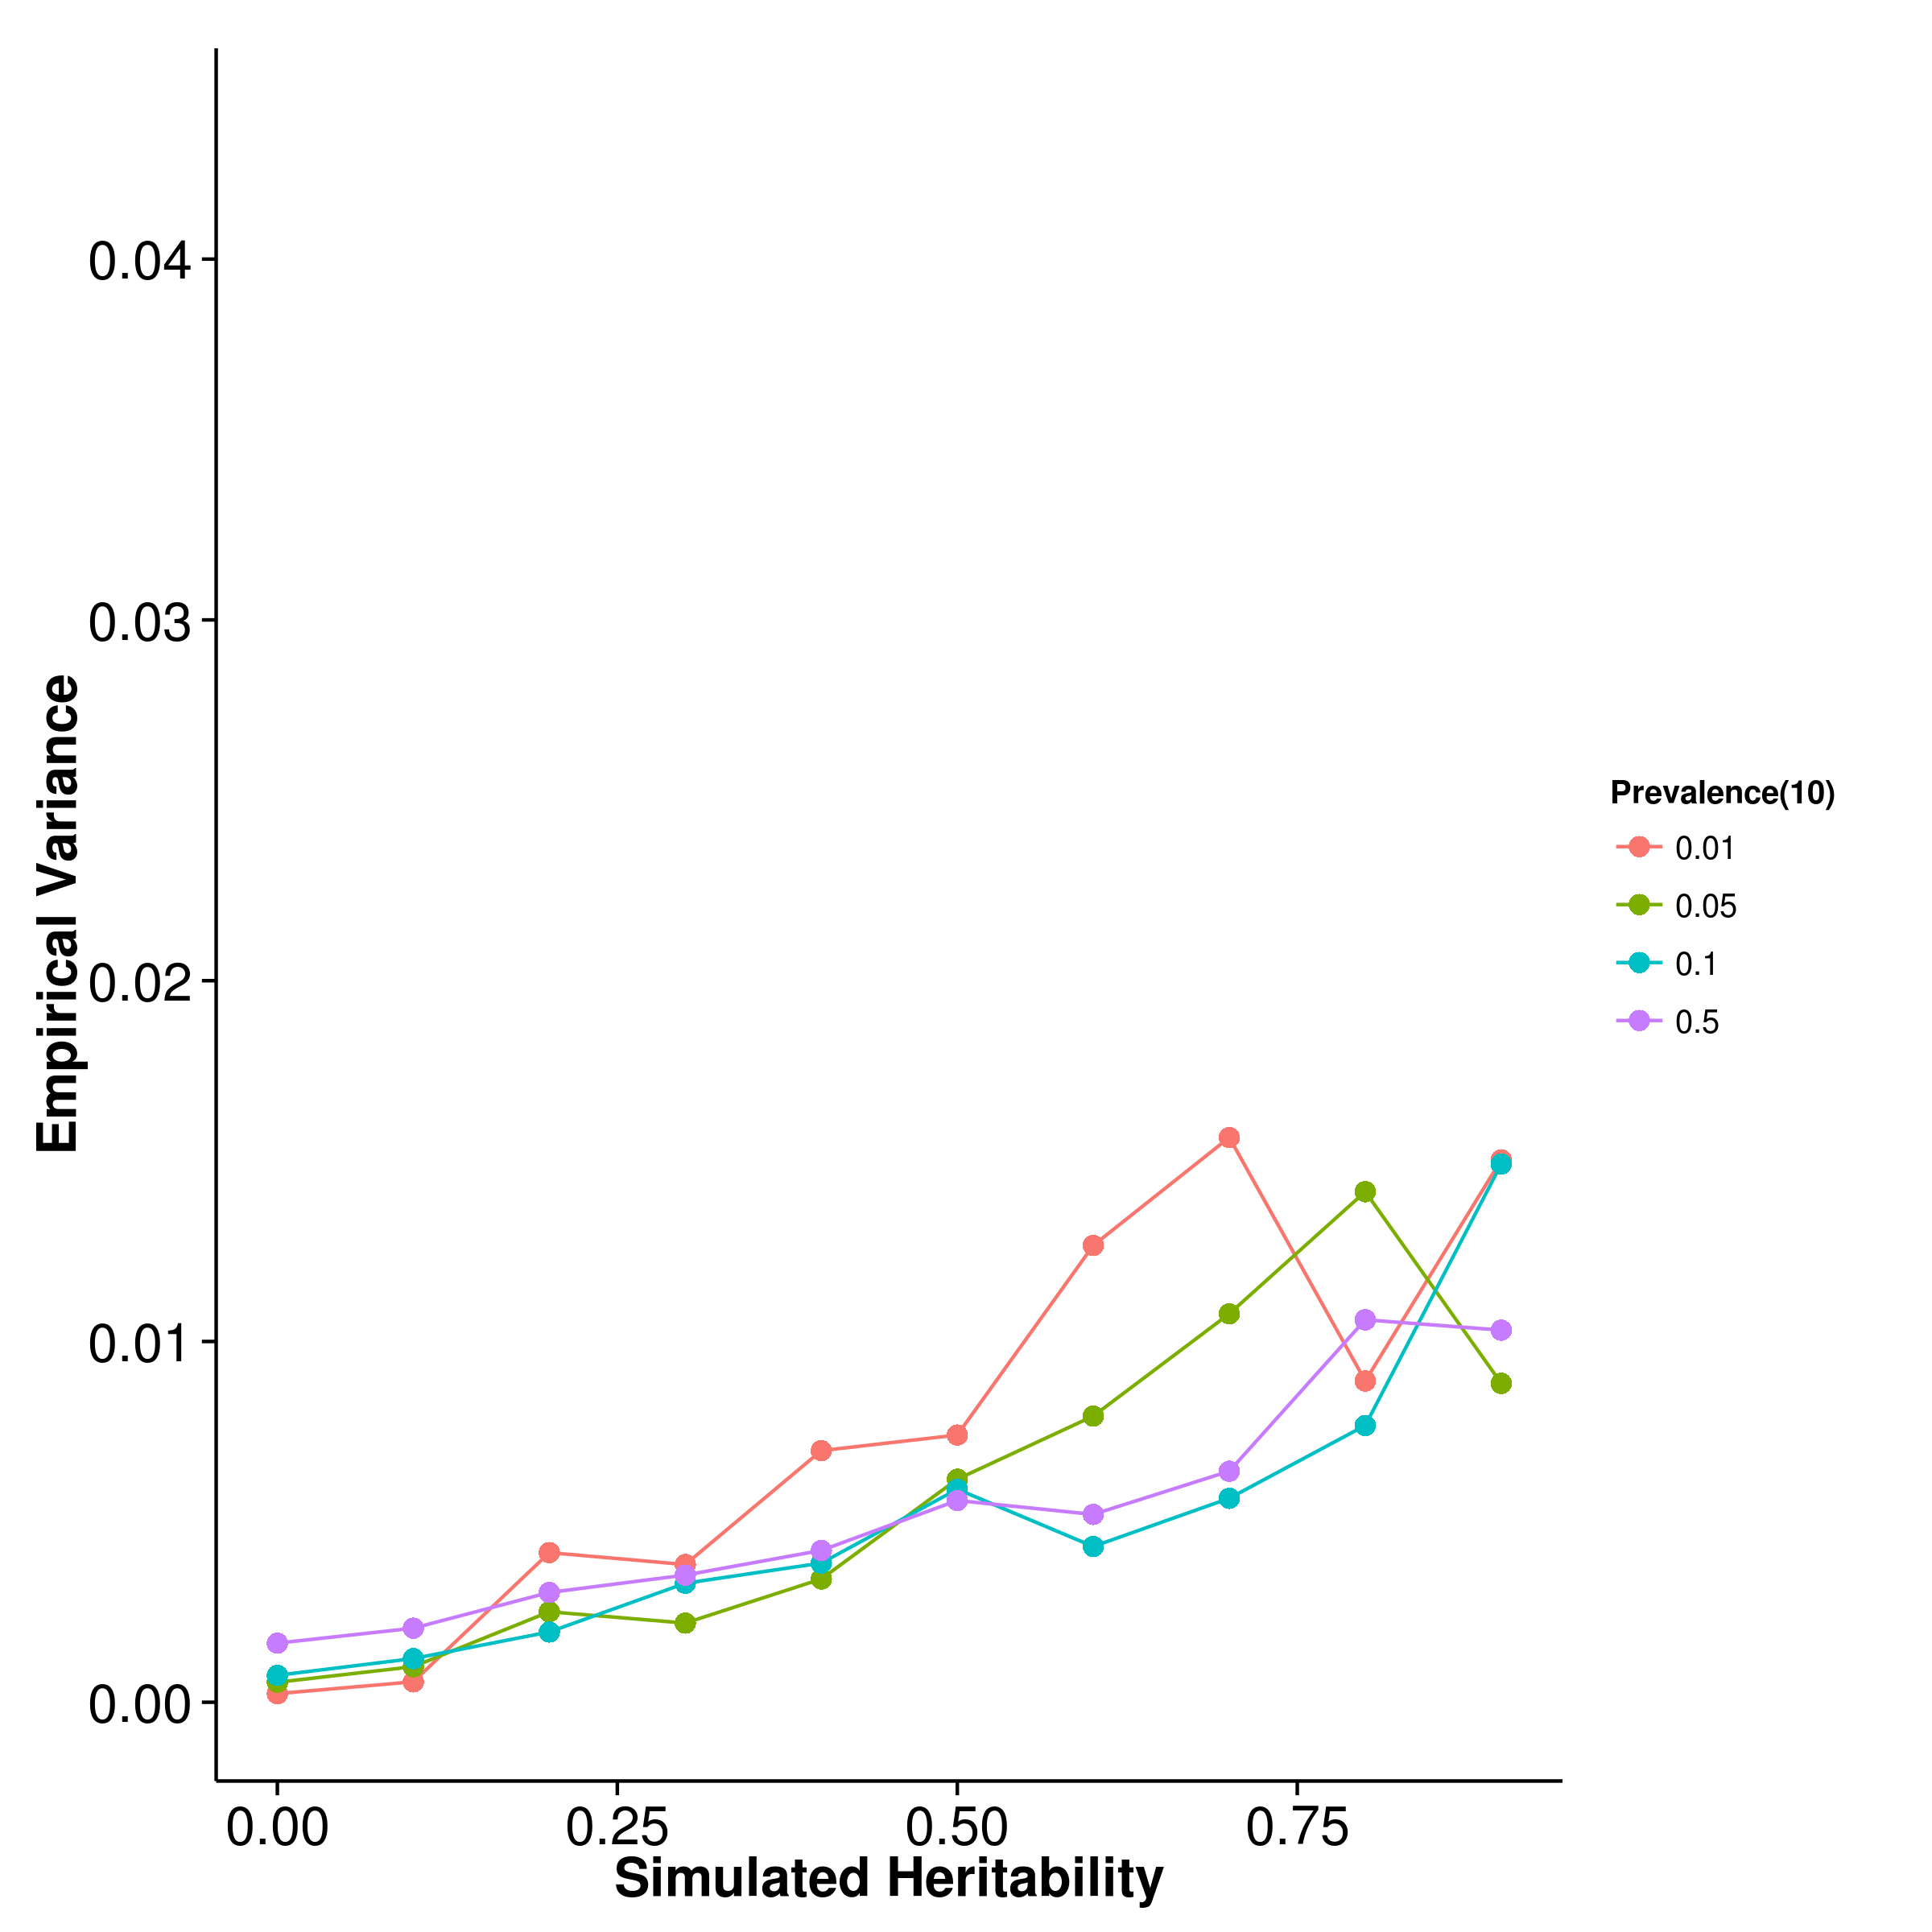
\includegraphics{figure/he_summary/cc_10c/shrek_CC_Rand_sd.png}}
				\label{fig:shrekCC10RandVar}
			}
			\subfloat[GCTA]{
				\scalebox{.4}{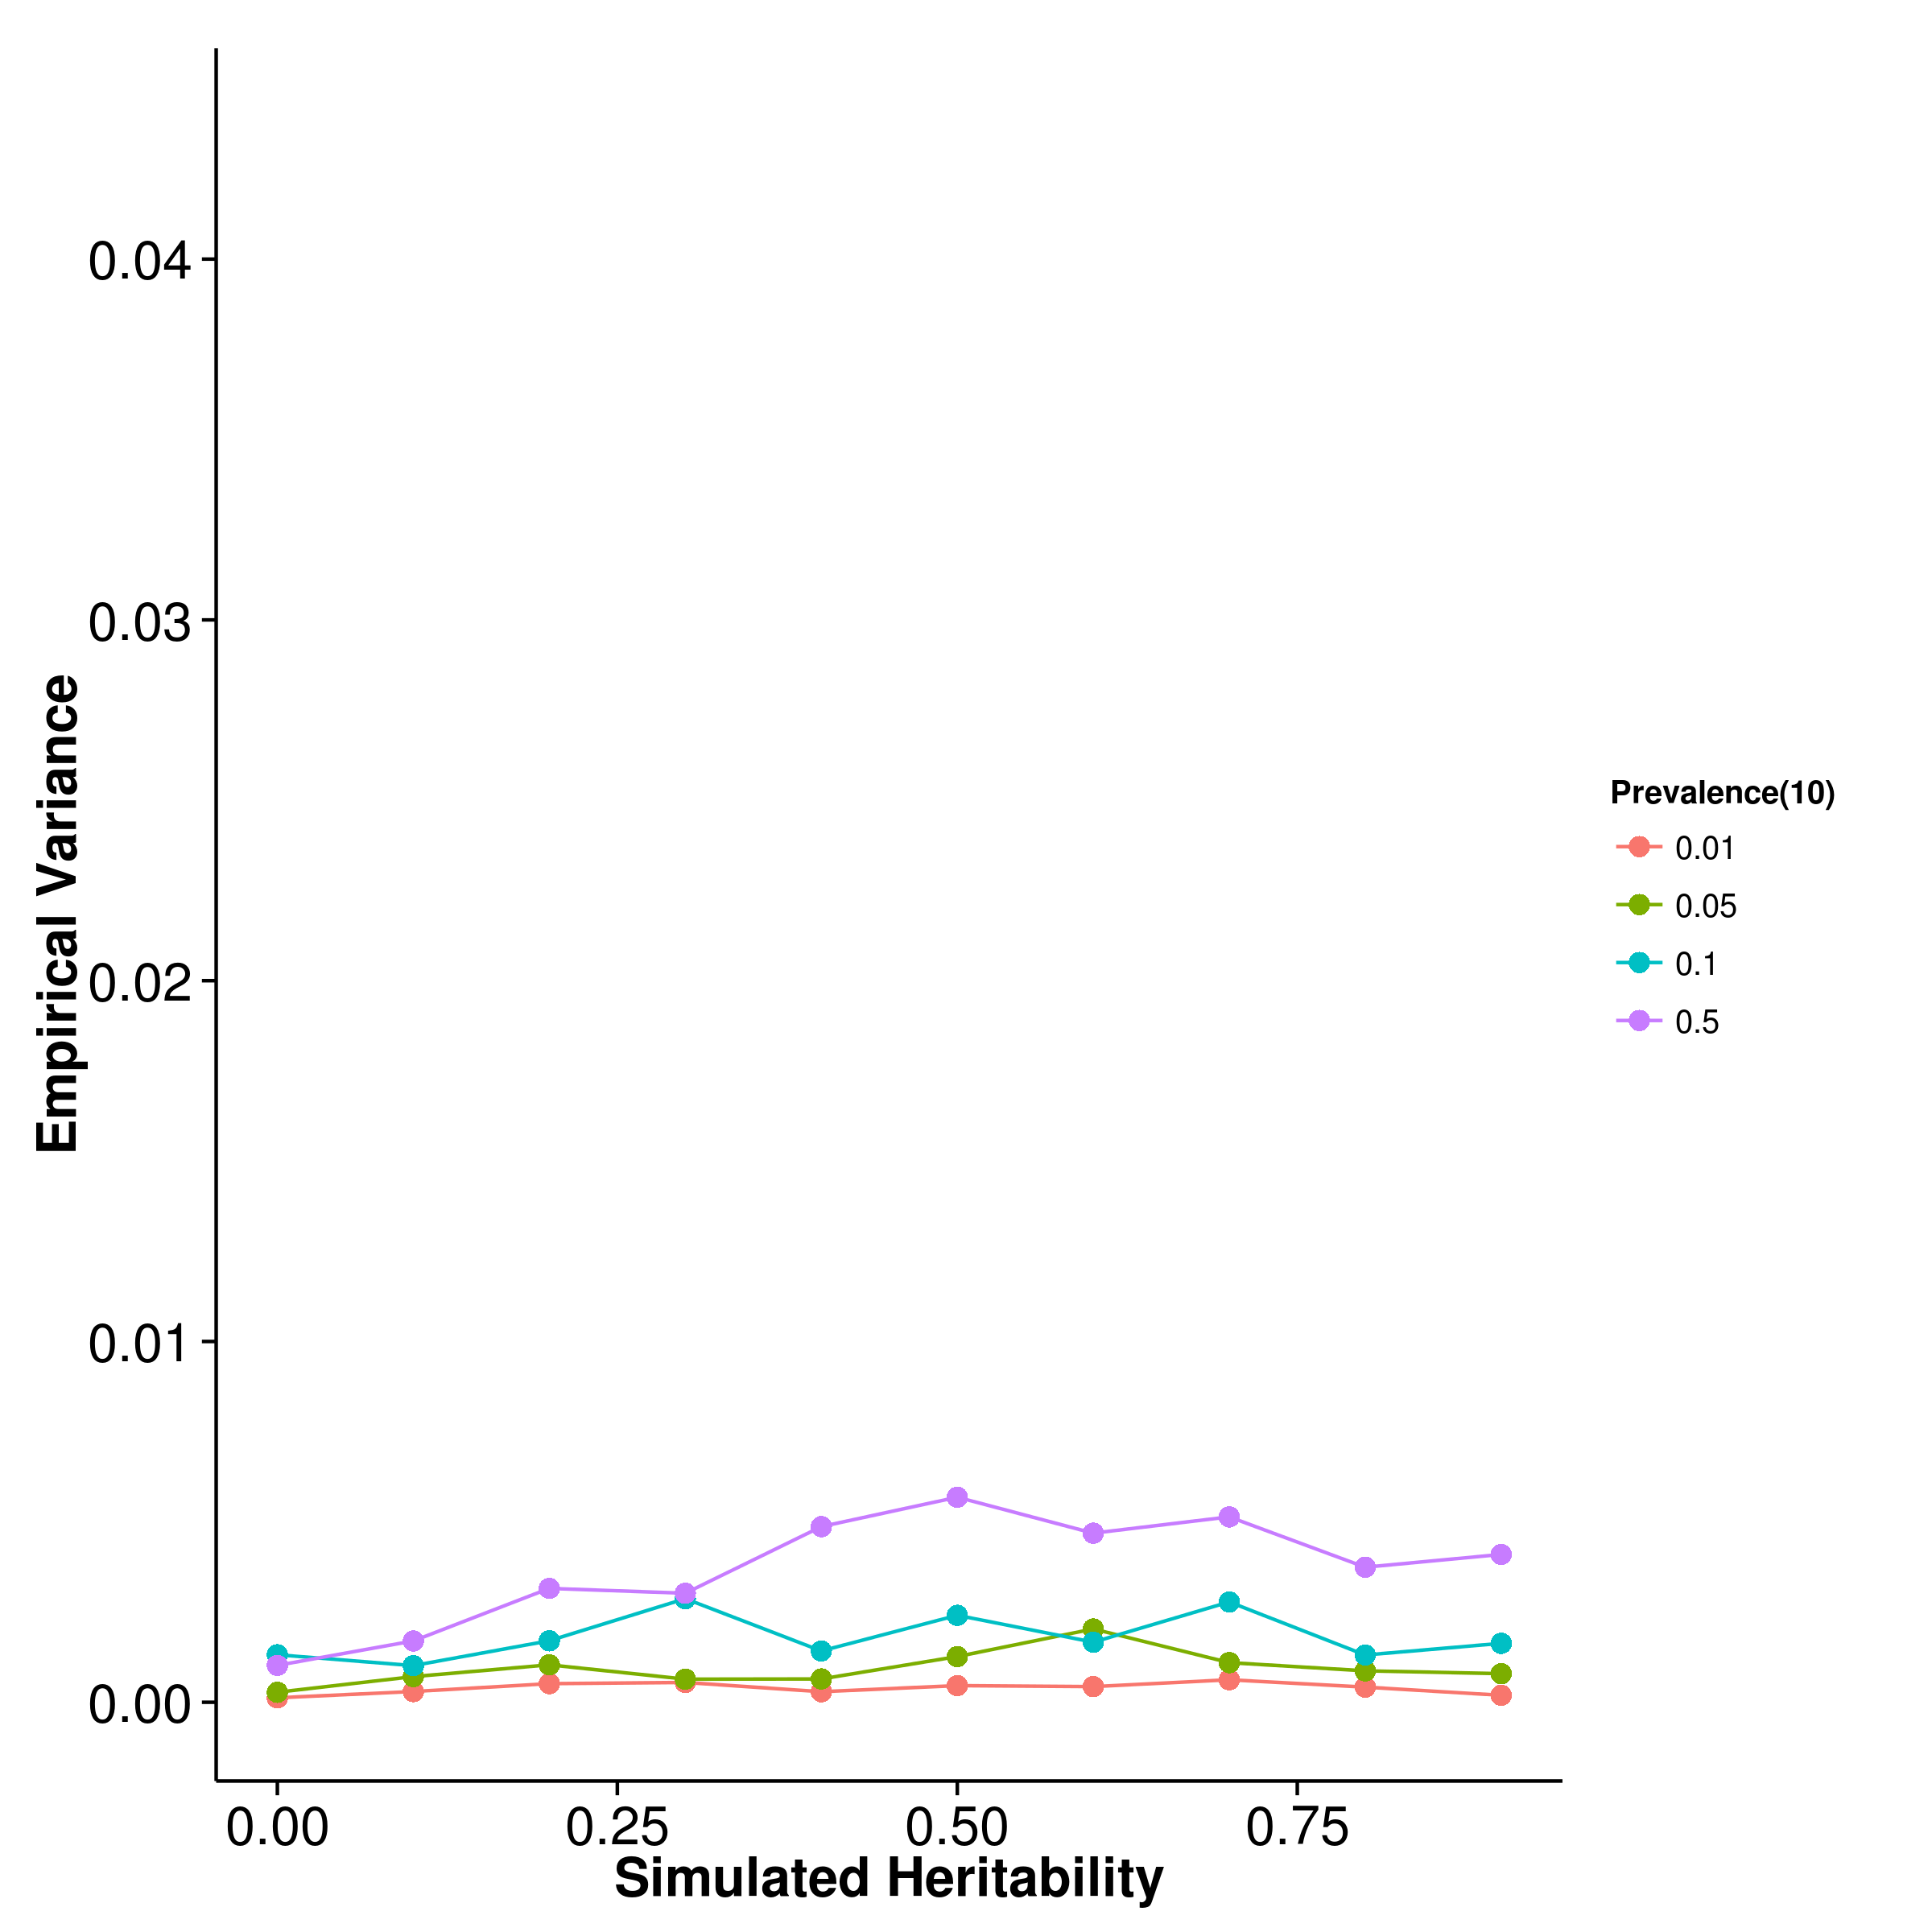
\includegraphics{figure/he_summary/cc_10c/gcta_CC_Rand_sd.png}}
				\label{fig:gctaCC10RandVar}
			}\\
			\subfloat[LDSC with fix intercept]{
				\scalebox{.4}{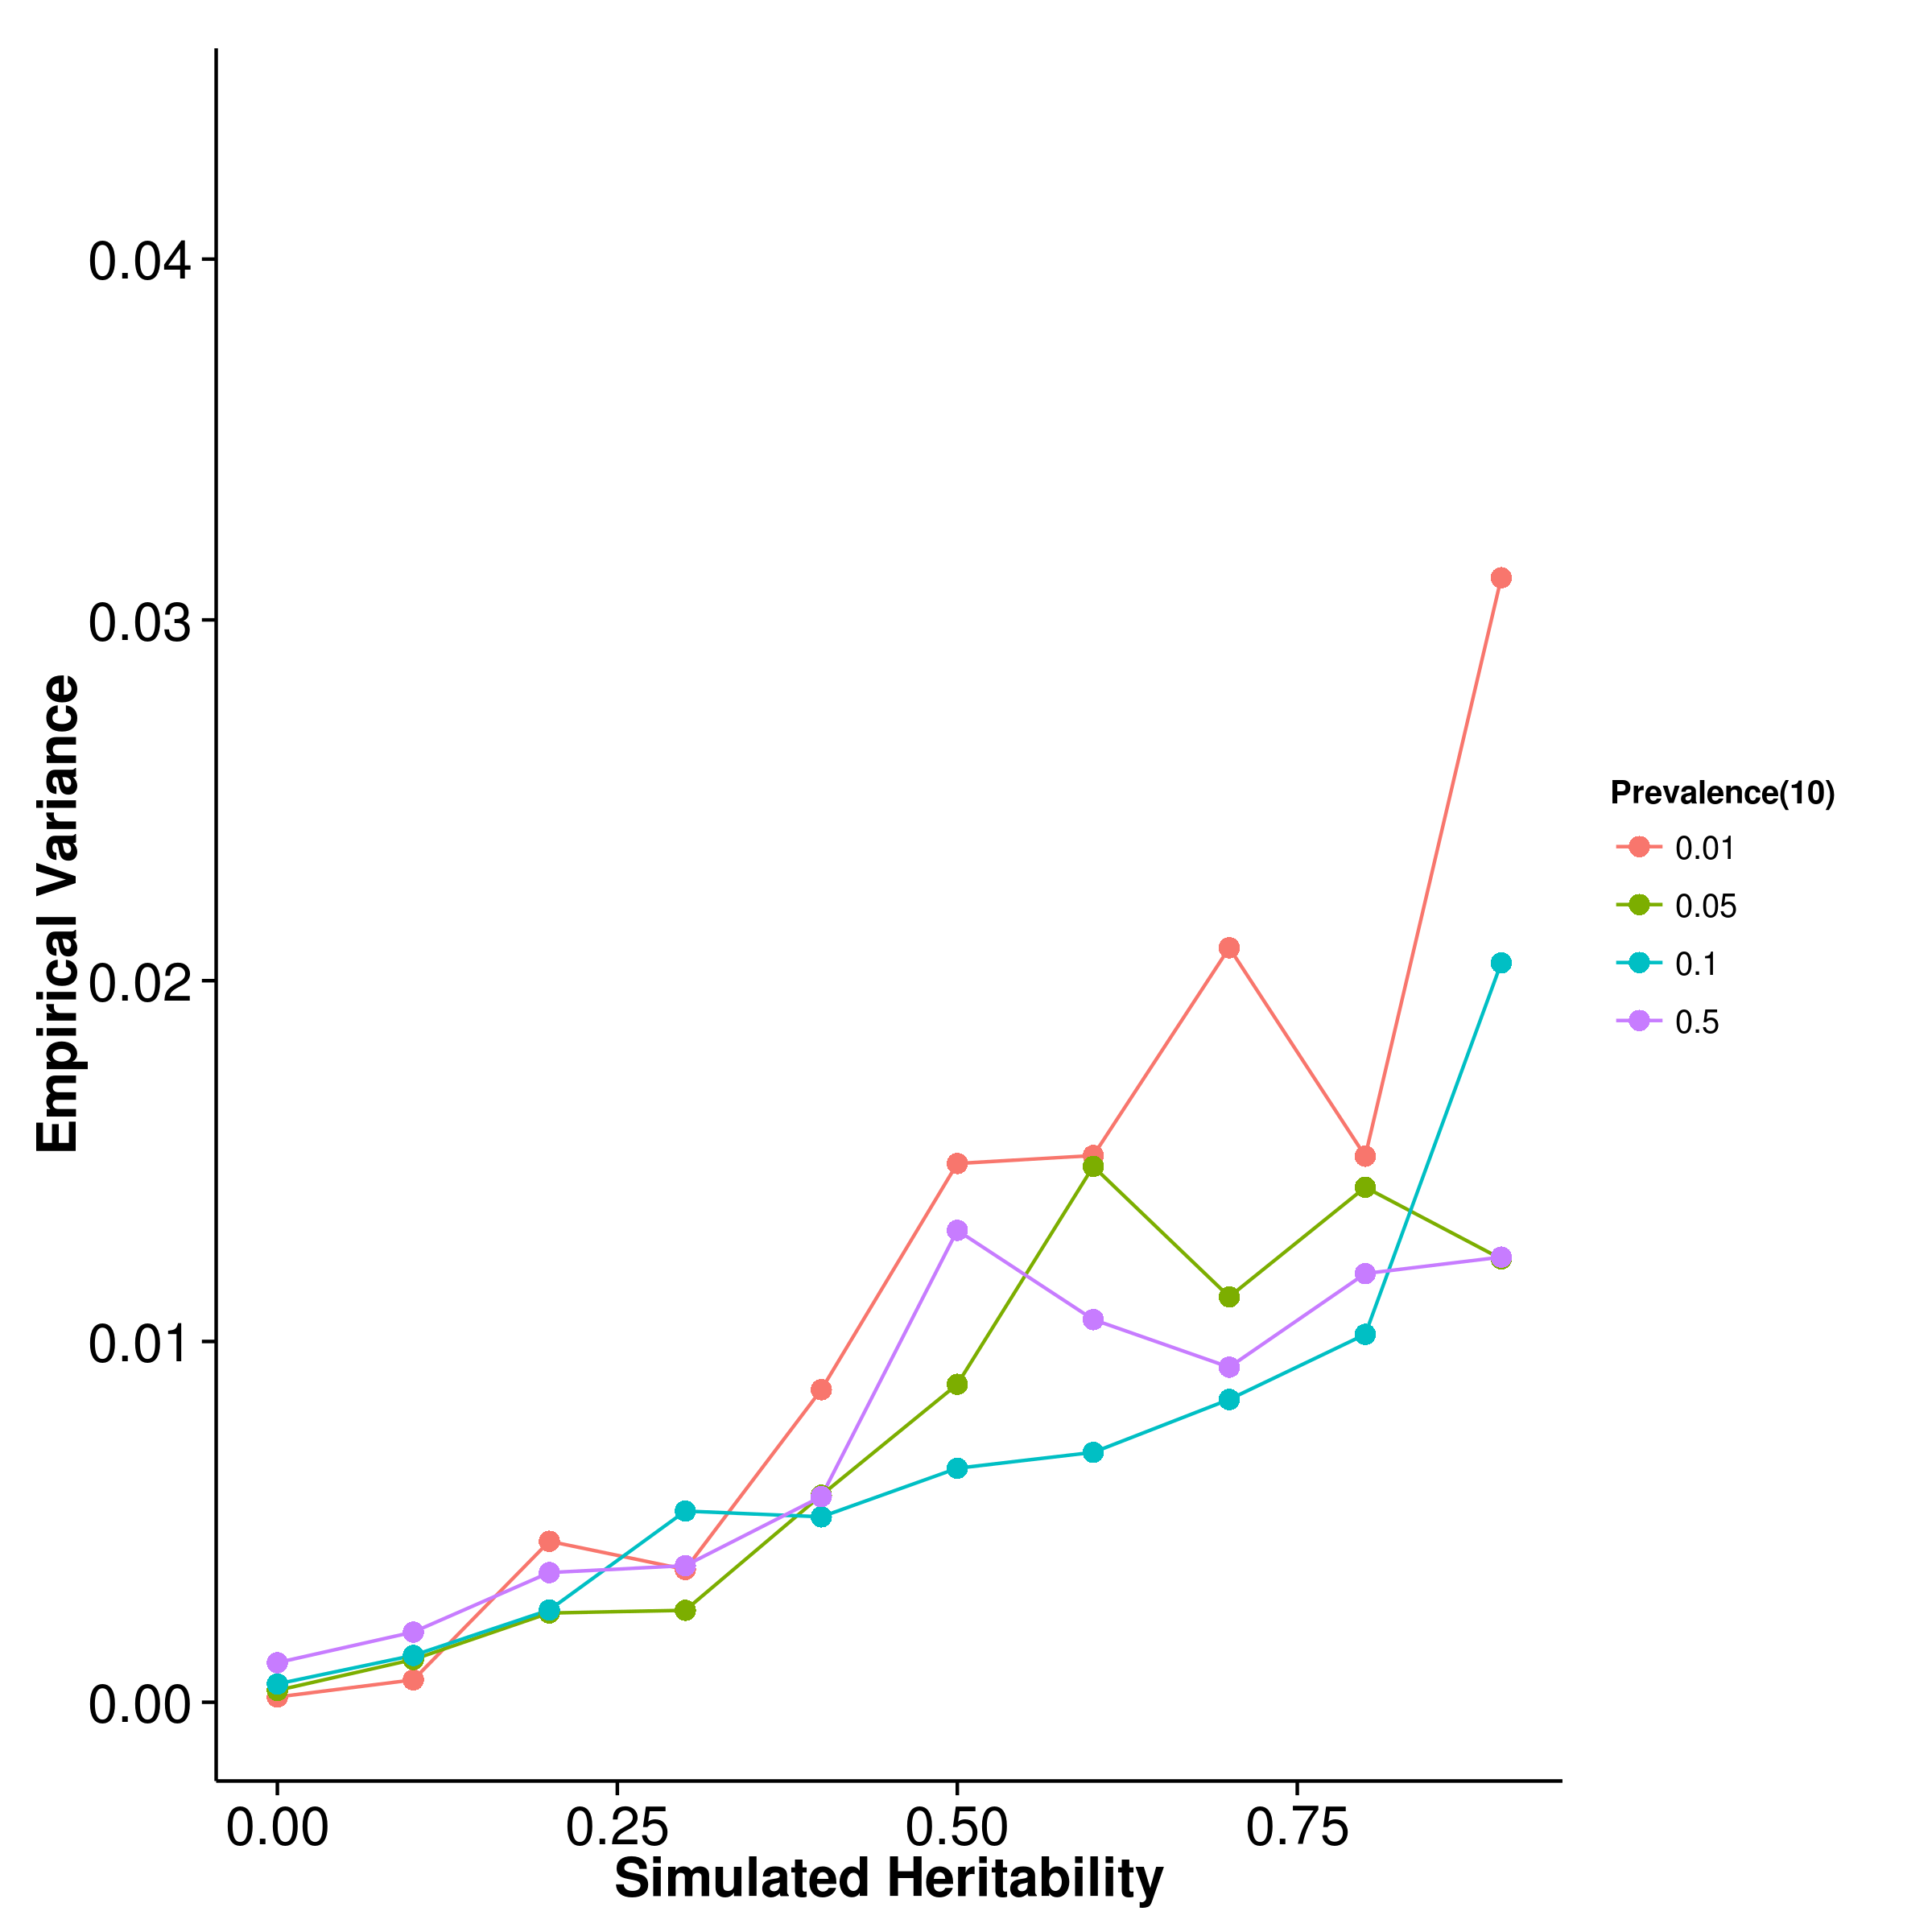
\includegraphics{figure/he_summary/cc_10c/ldsc_CC_Rand_sd.png}}
				\label{fig:ldscCC10RandVar}
			}
			\subfloat[LDSC with intercept estimation]{
				
				\scalebox{.4}{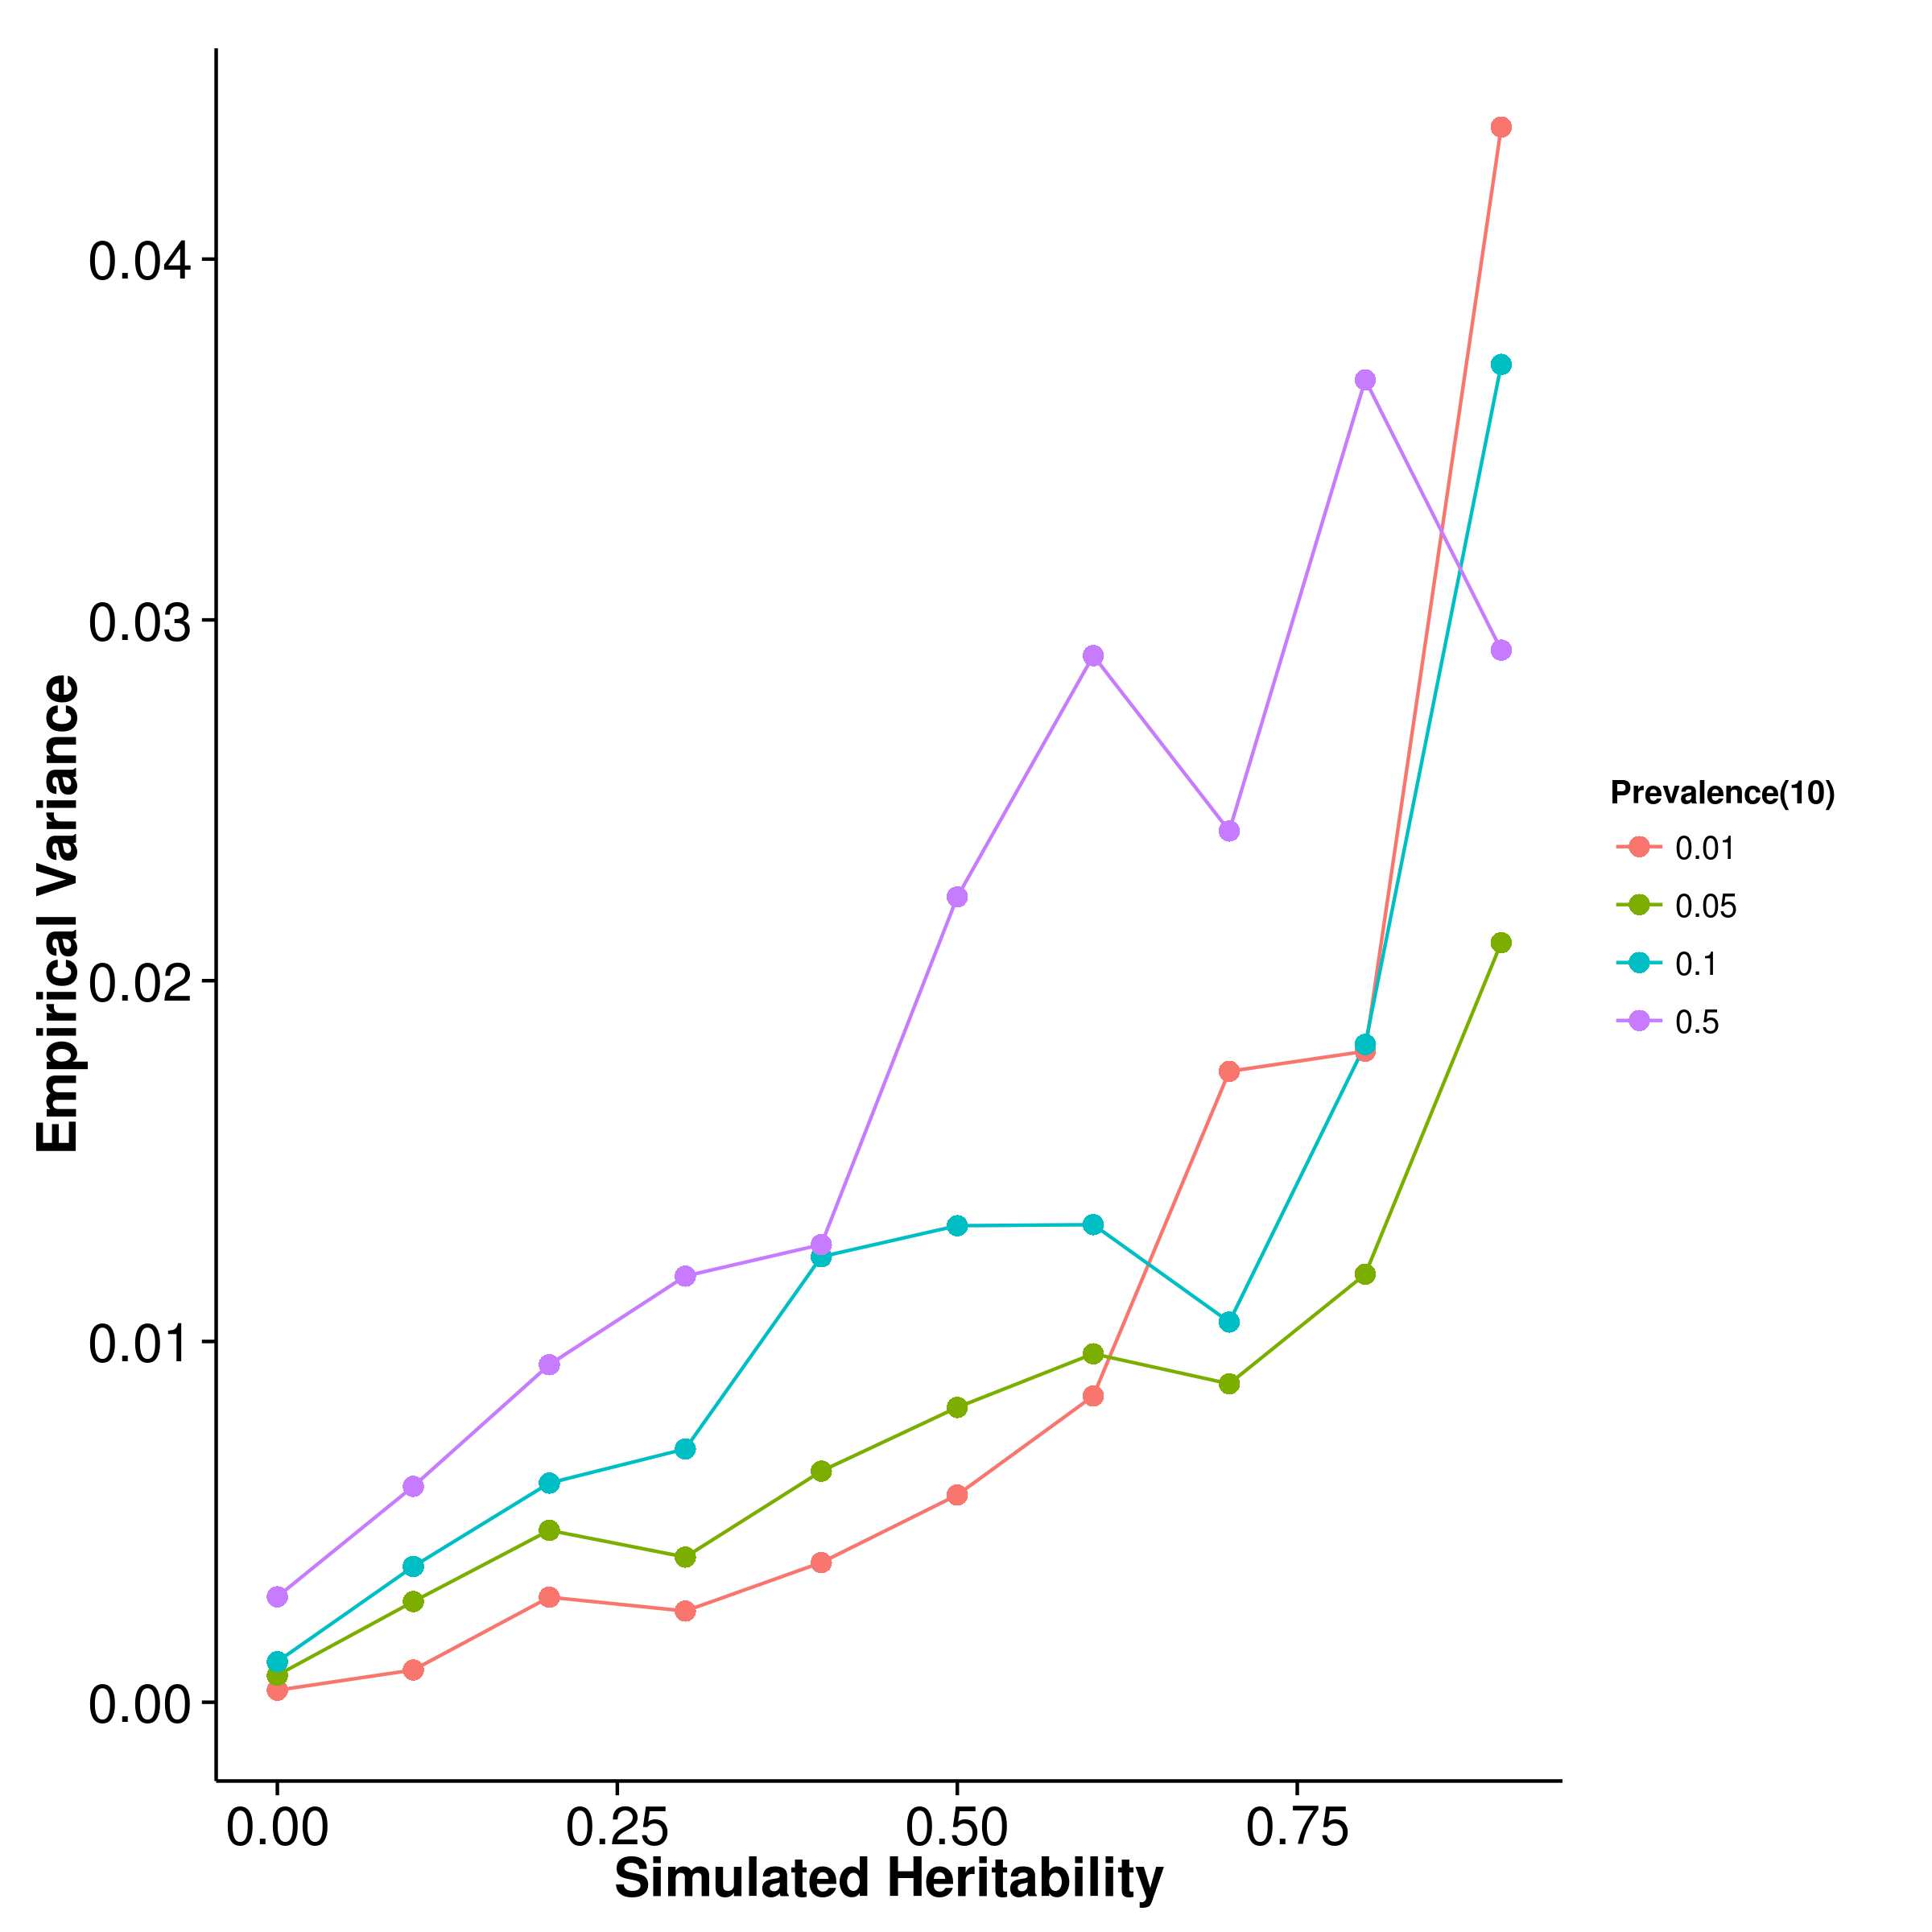
\includegraphics{figure/he_summary/cc_10c/ldscIn_CC_Rand_sd.png}}
				\label{fig:ldscInCC10RandVar}
			}
			\caption[Variance of Case Control Simulation Results (10 Causal)]
			{Variance of results from case control simulation with random effect size simulation with 10 causal \glspl{SNP}.
				There were no clear pattern as to how the prevalence affect the empirical variance of estimates from \gls{shrek} and \gls{ldsc}. 
				For \gls{gcta}, it seems like a larger prevalence tends to result in a larger empirical variance. 
				Again, \gls{gcta} has the lowest variance, follow by \gls{shrek} and \gls{ldsc} with fixed intercept.
				Nonetheless, it was important to remember that in case control simulation, a much smaller amount of \glspl{SNP} was used, thus the results was not directly comparable to results from the quantitative simulation.
			} 
			\label{fig:CC10RandVar}
		\end{figure}
		
		
		\begin{figure}
			\centering
			\subfloat[SHREK]{
				\scalebox{.4}{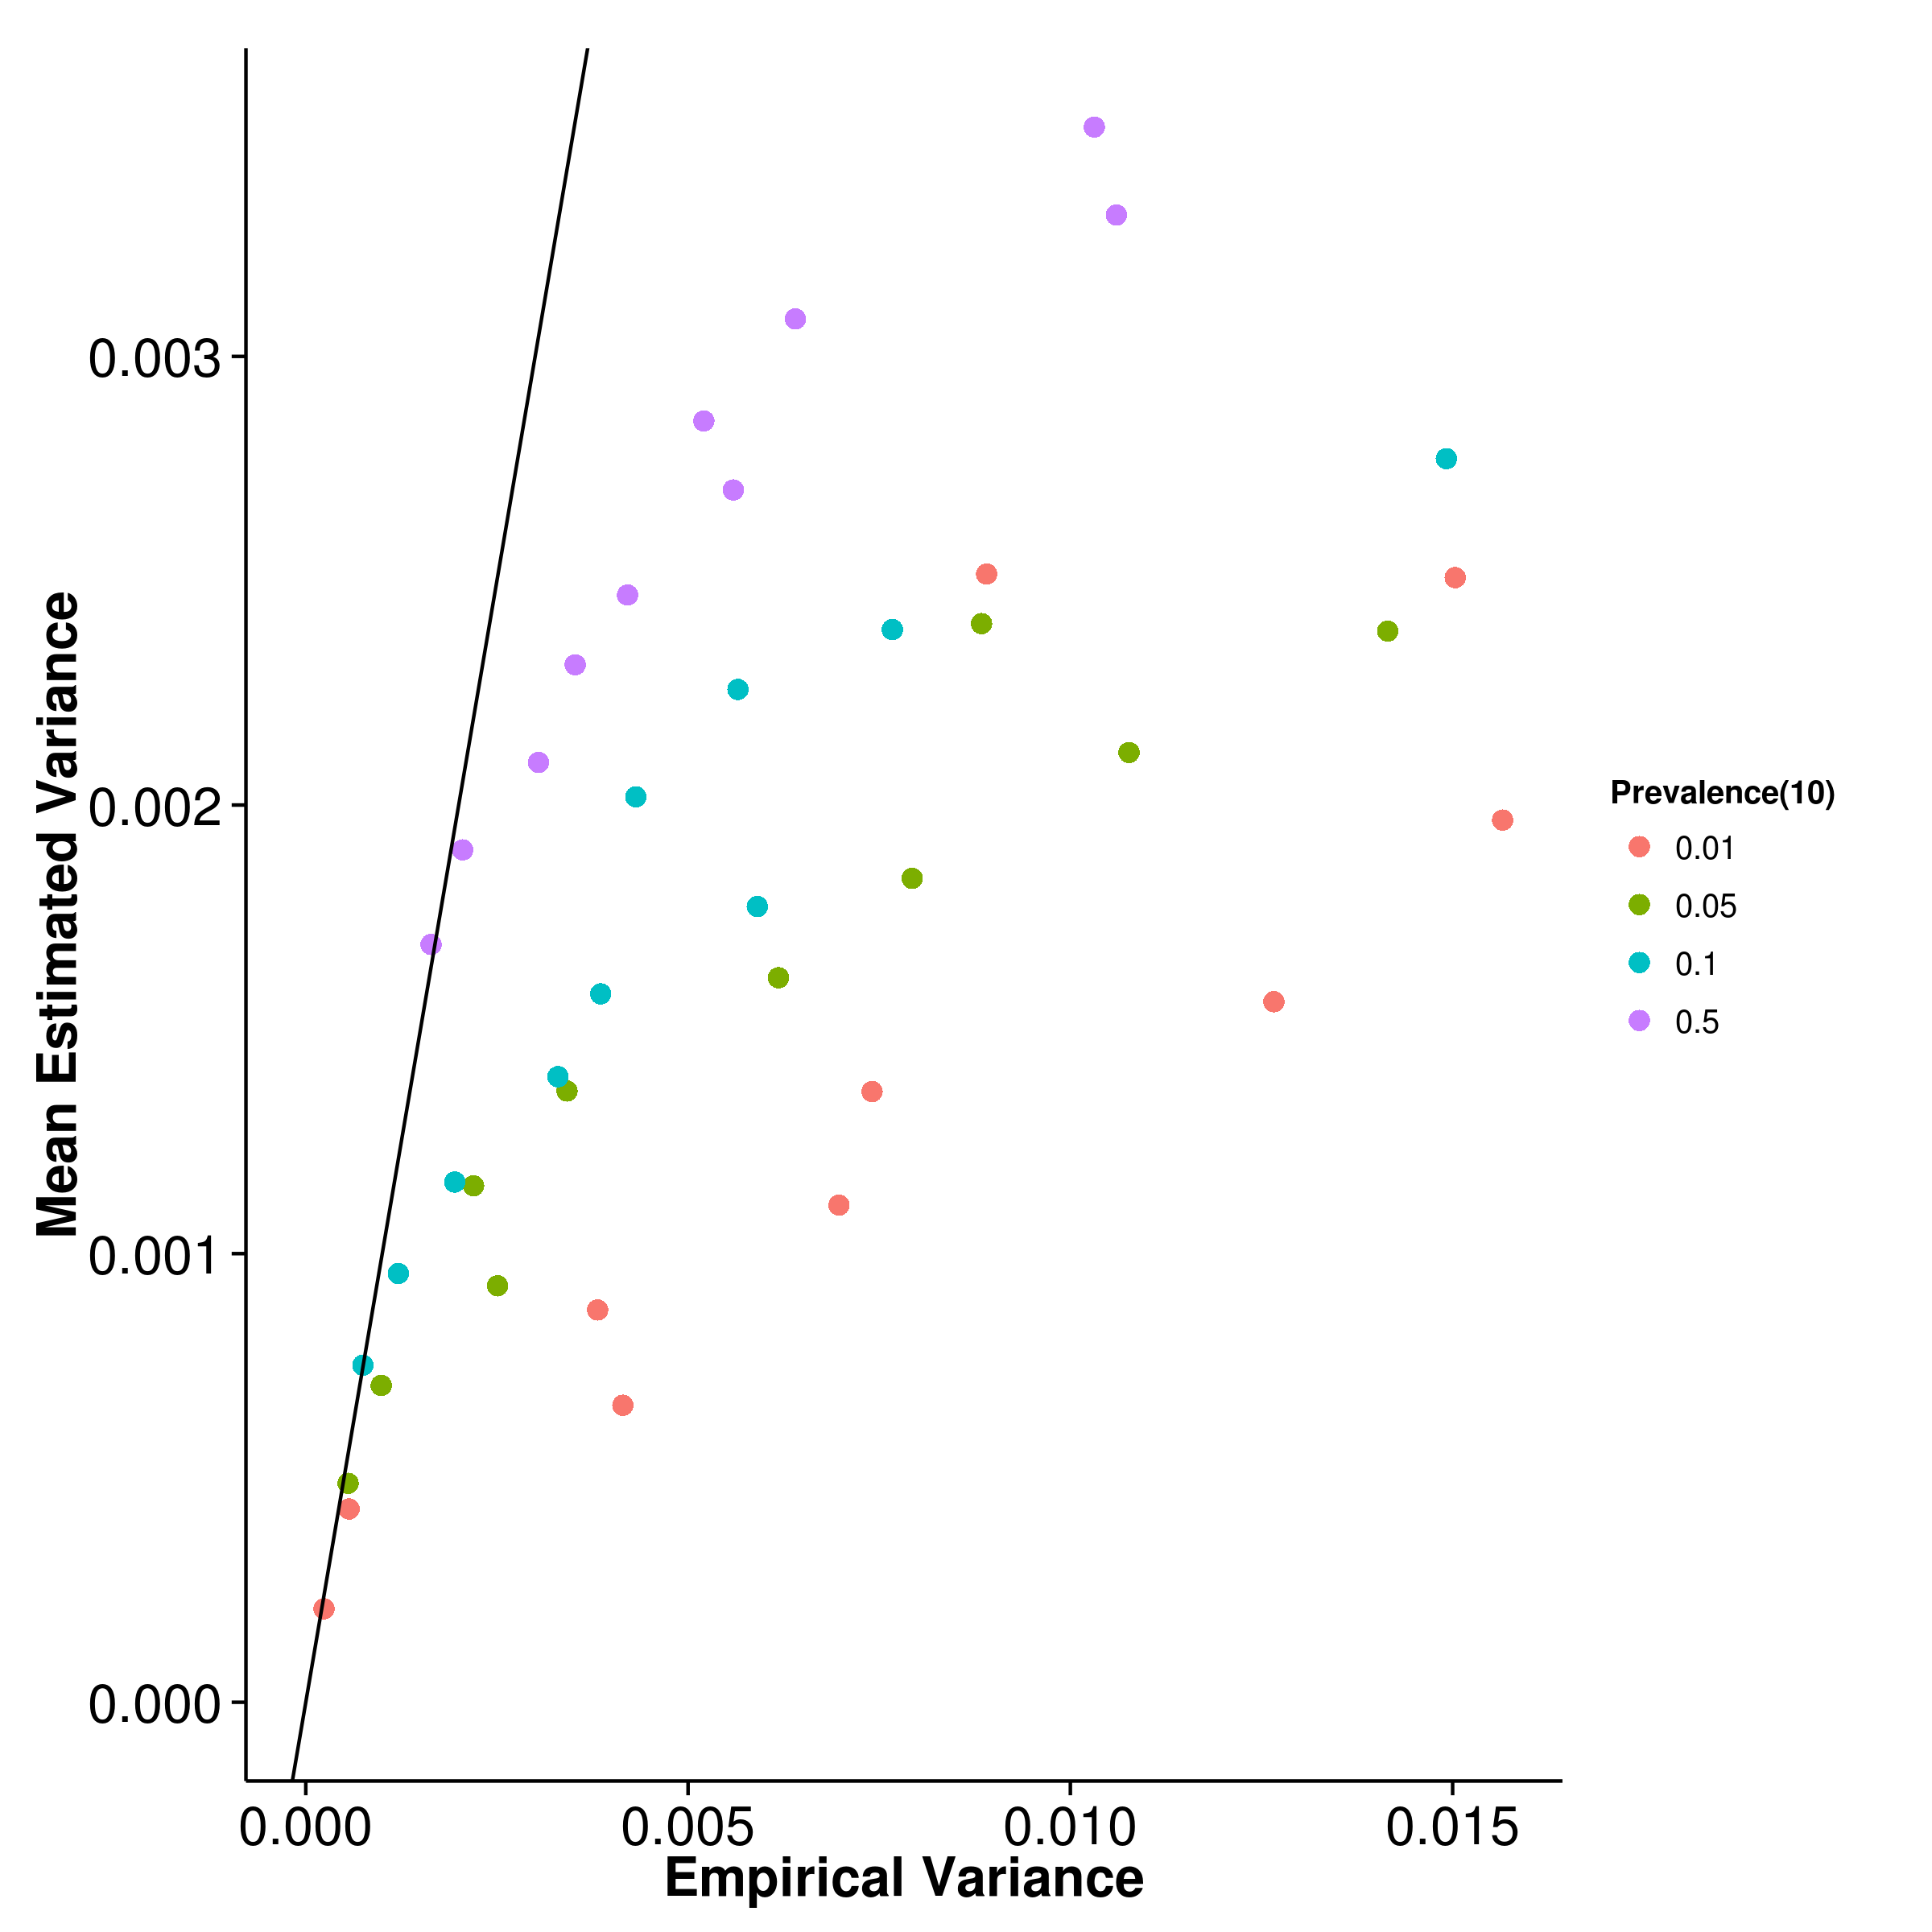
\includegraphics{figure/he_summary/cc_10c/shrek_CC_Rand_sdCom.png}}
				\label{fig:shrekCC10RandVarCom}
			}
			\subfloat[GCTA]{
				\scalebox{.4}{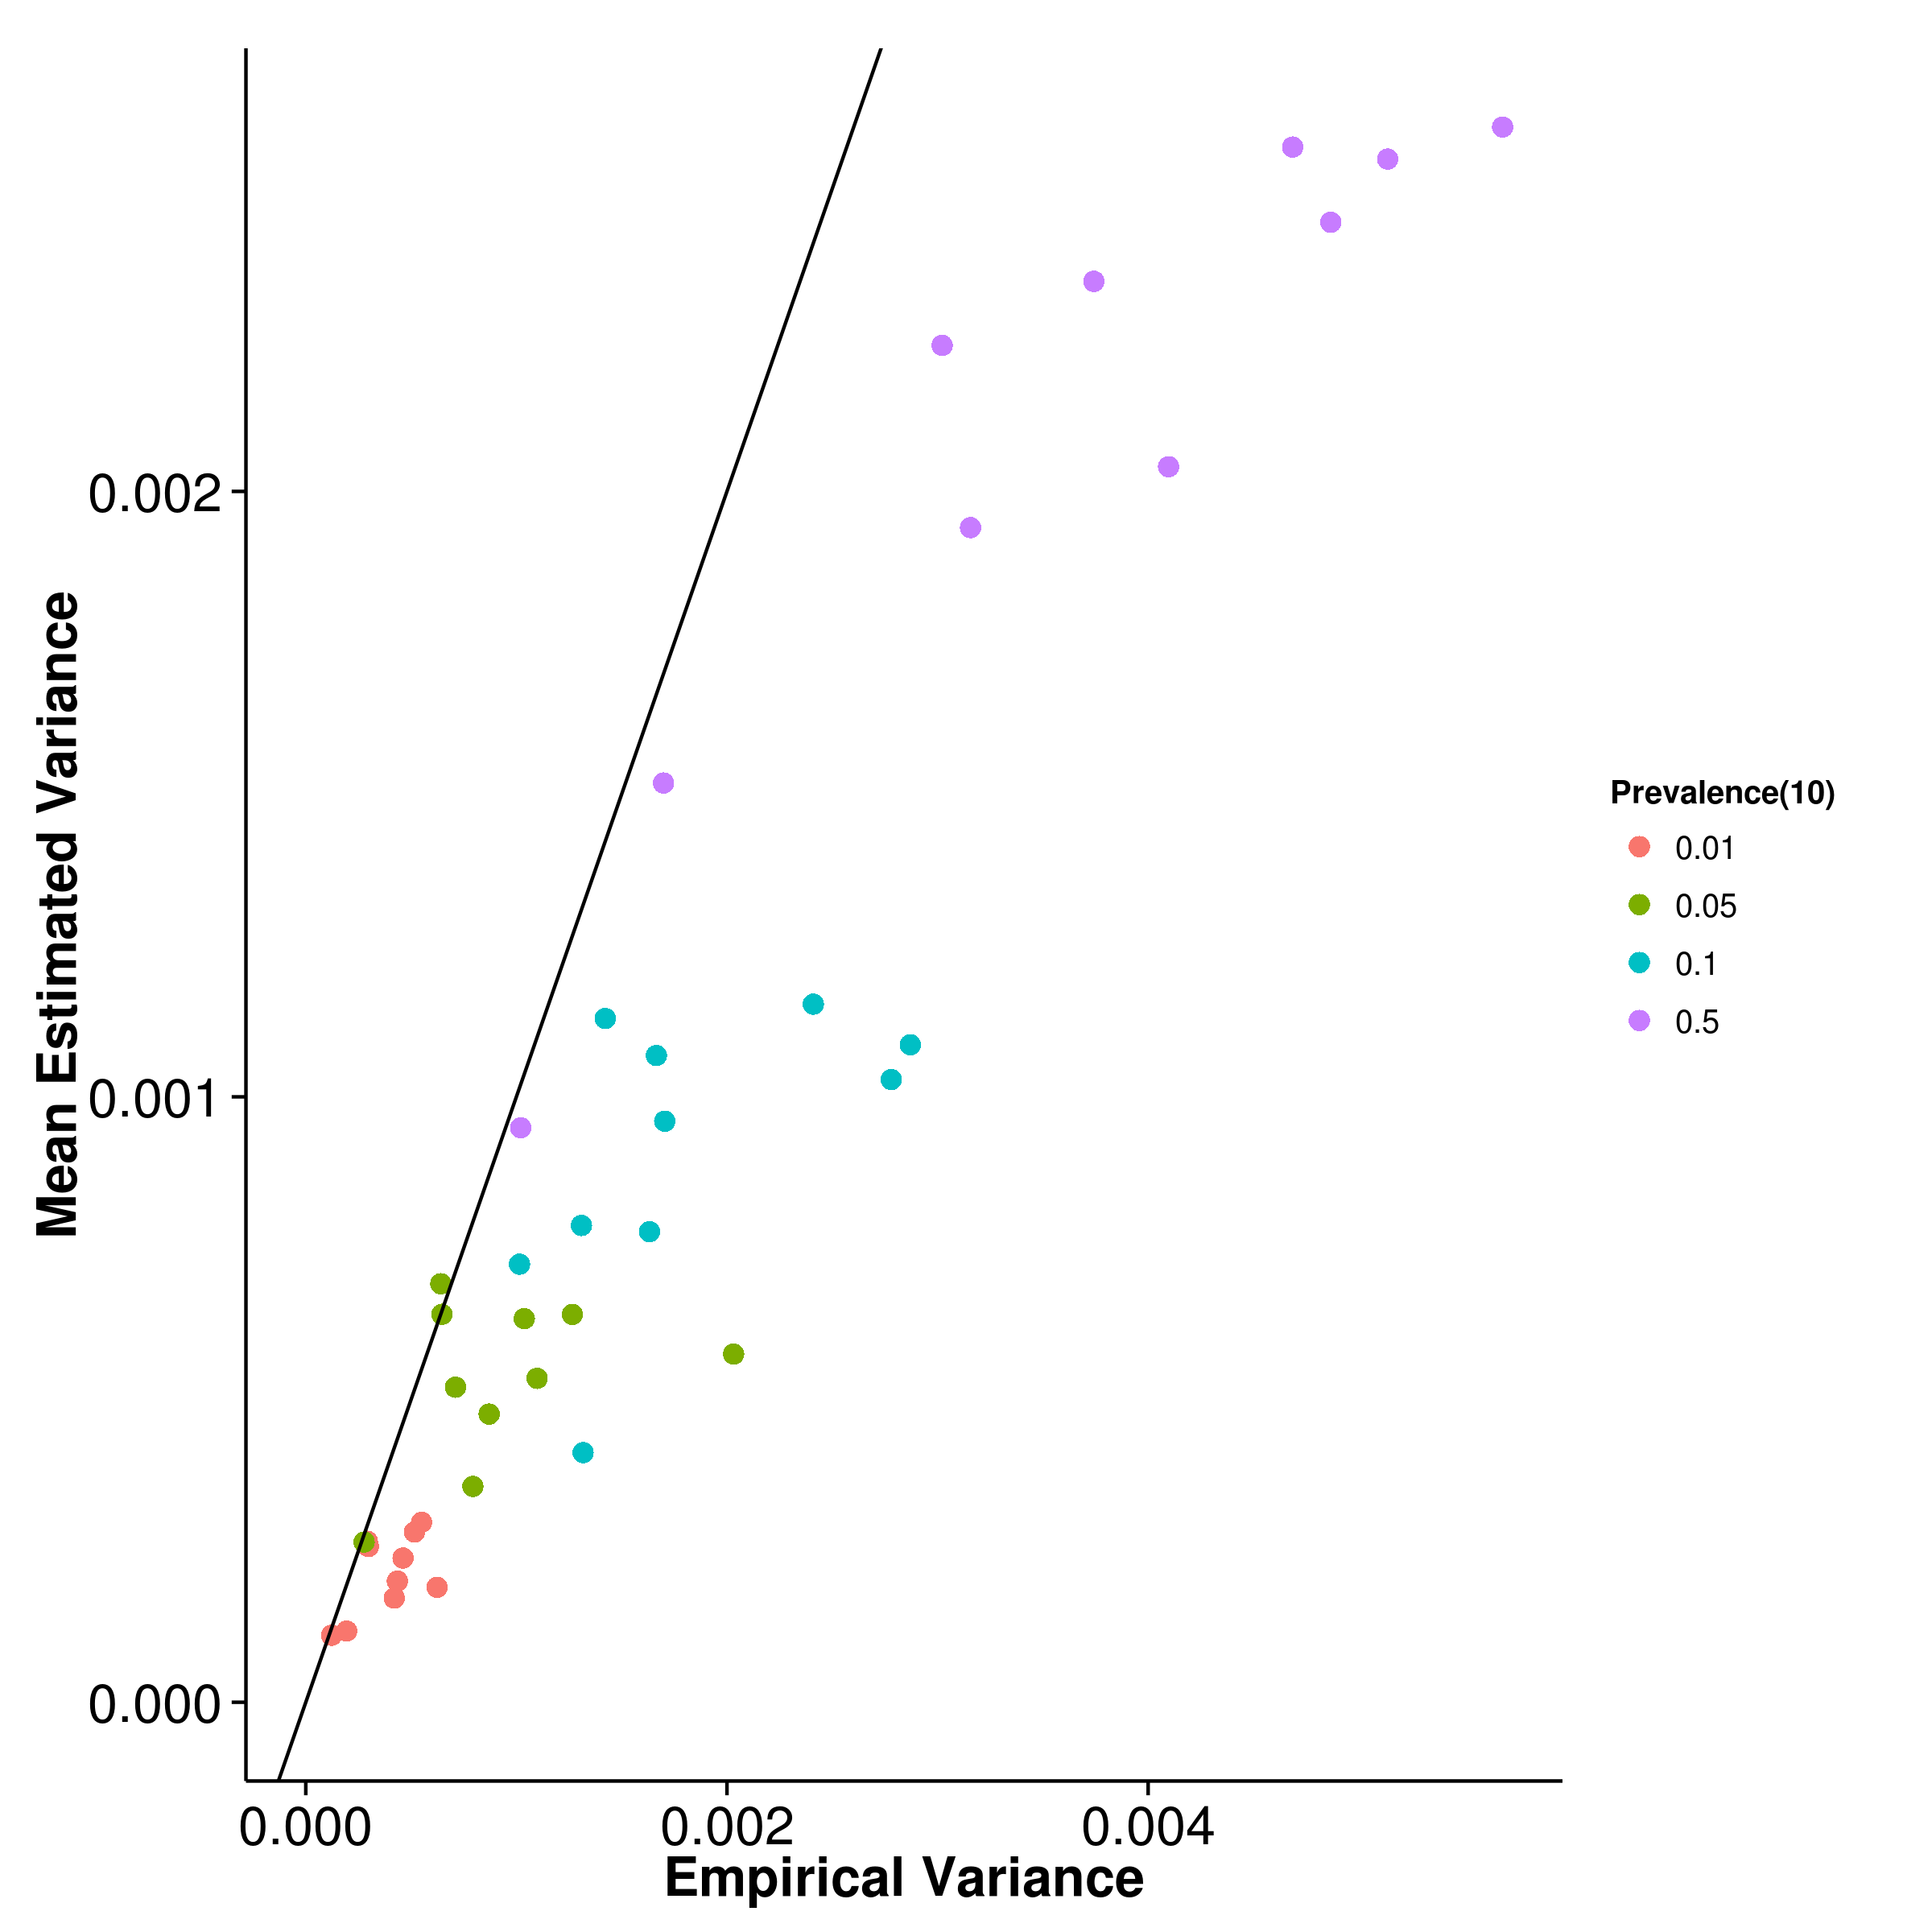
\includegraphics{figure/he_summary/cc_10c/gcta_CC_Rand_sdCom.png}}
				\label{fig:gctaCC10RandVarCom}
			}\\
			\subfloat[LDSC with fix intercept]{
				\scalebox{.4}{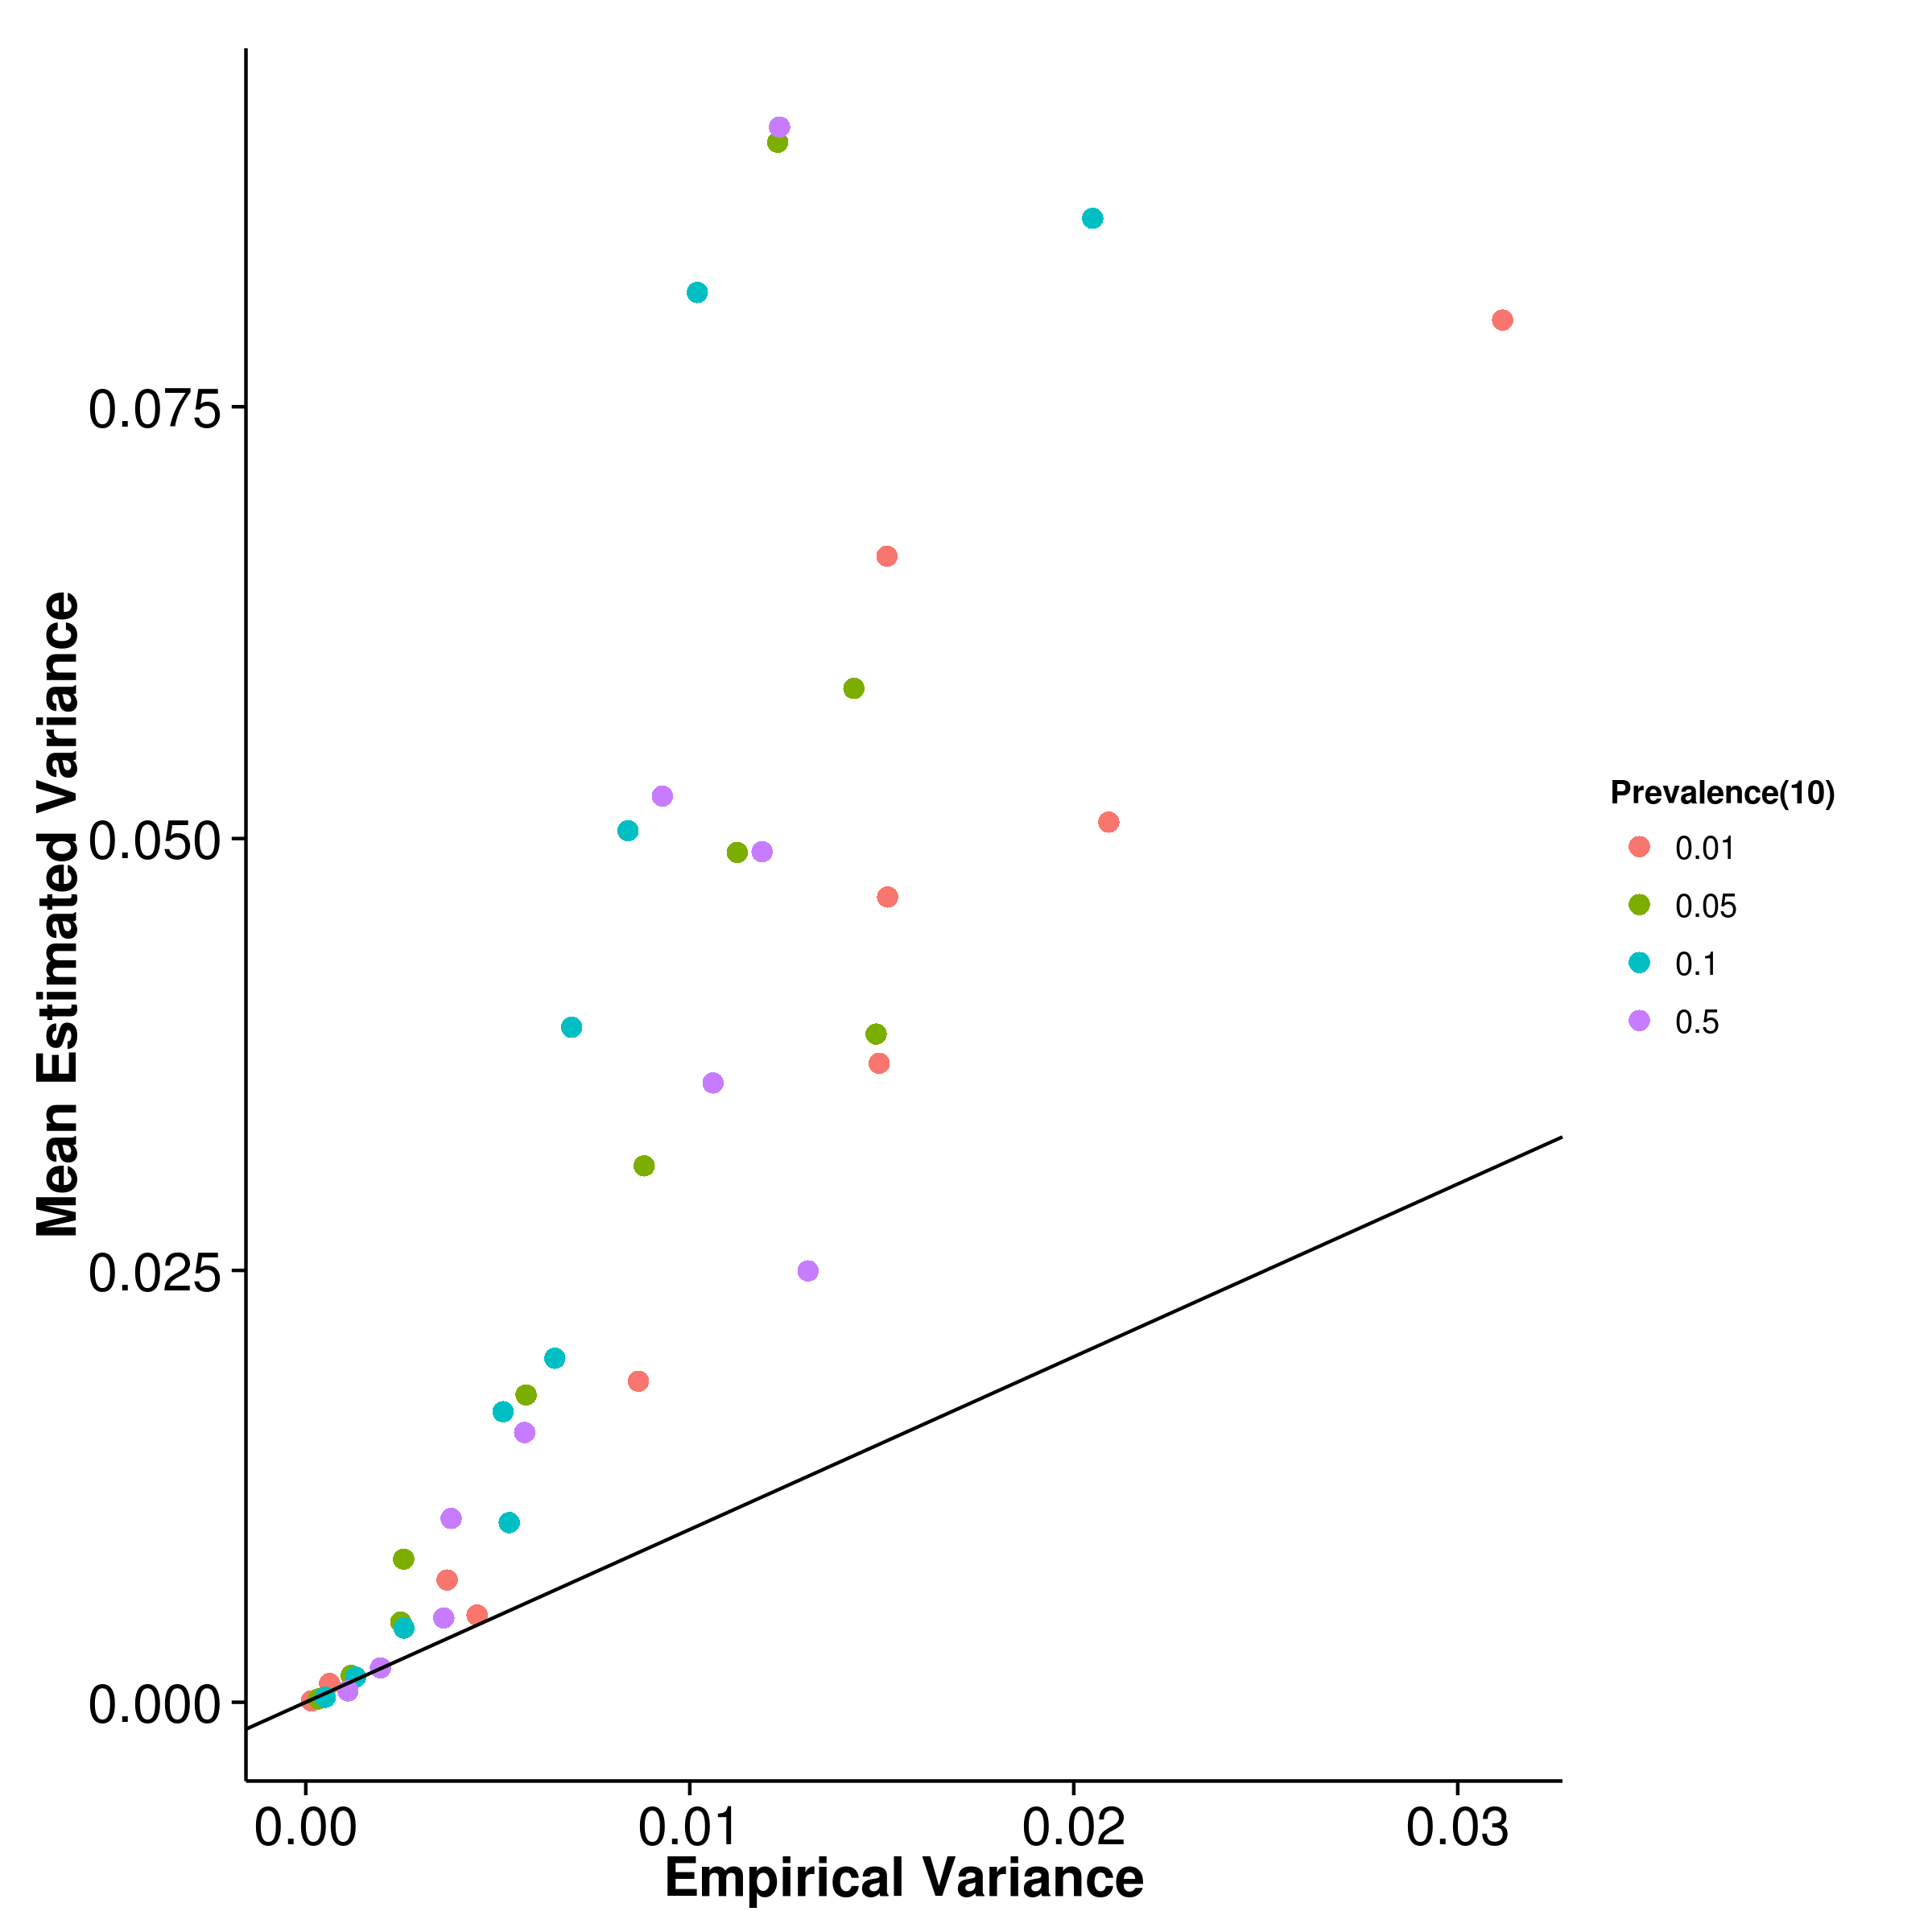
\includegraphics{figure/he_summary/cc_10c/ldsc_CC_Rand_sdCom.png}}
				\label{fig:ldscCC10RandVarCom}
			}
			\subfloat[LDSC with intercept estimation]{
				
				\scalebox{.4}{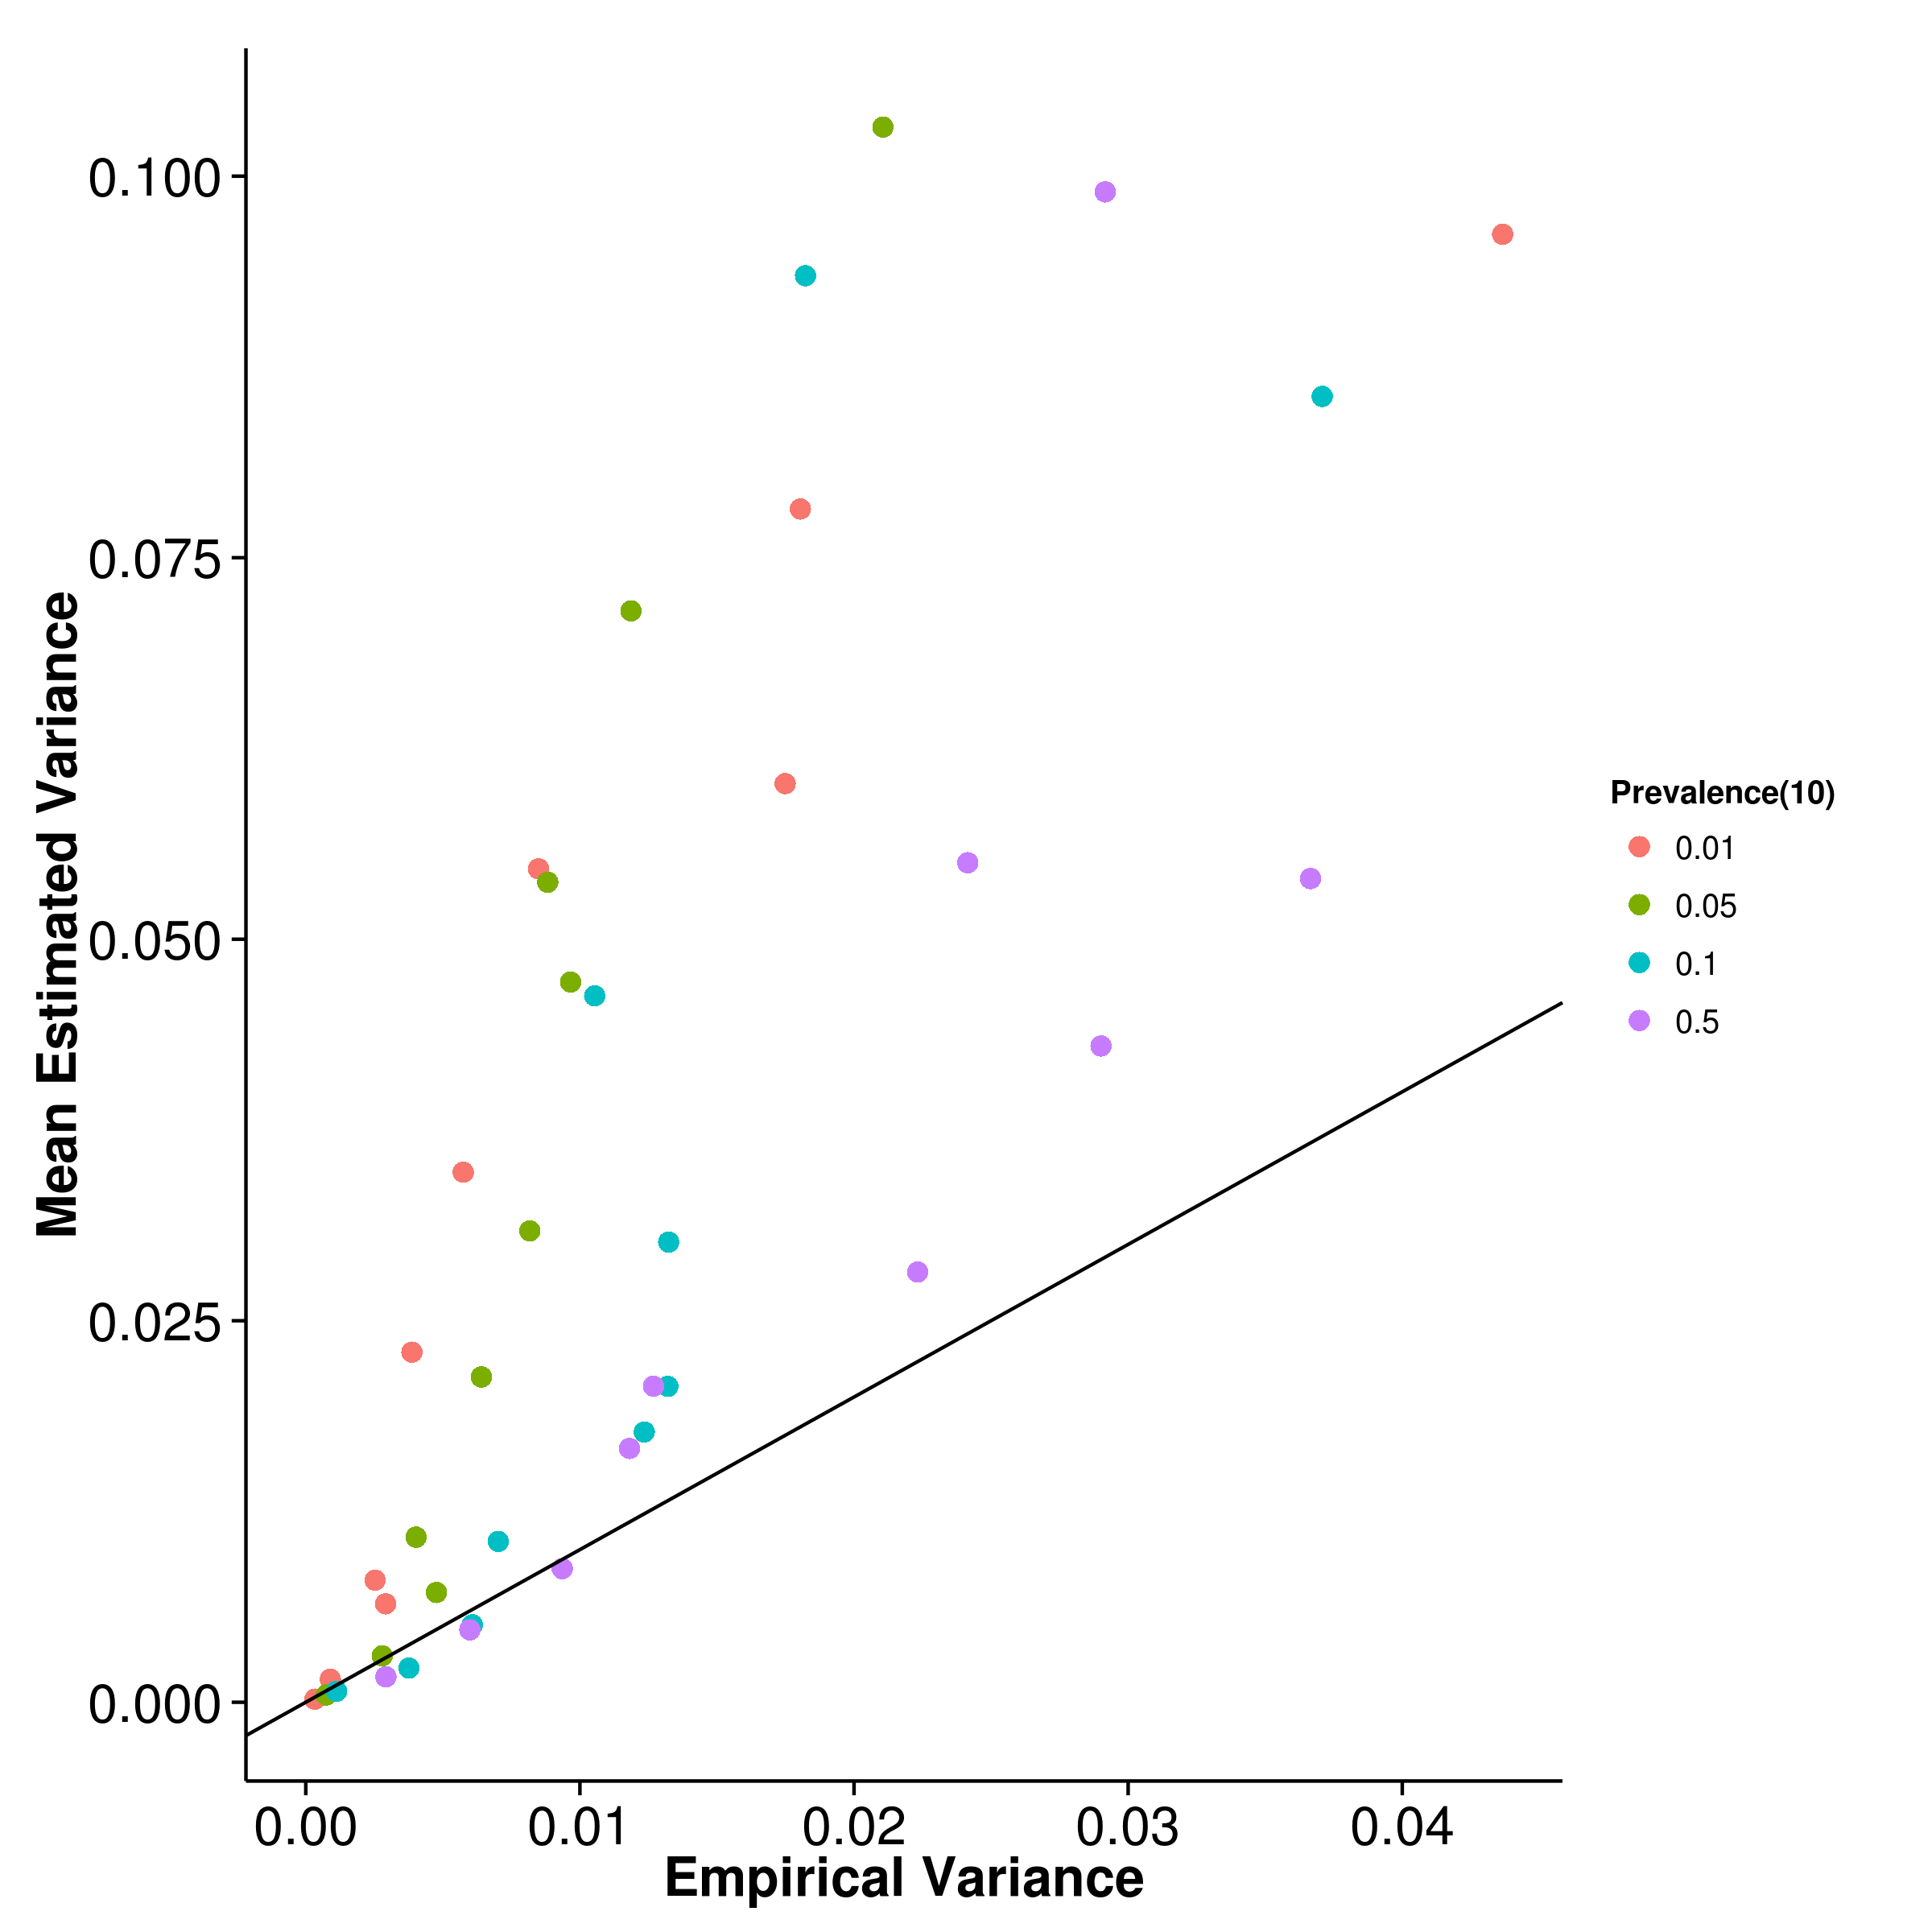
\includegraphics{figure/he_summary/cc_10c/ldscIn_CC_Rand_sdCom.png}}
				\label{fig:ldscInCC10RandVarCom}
			}
			\caption[Estimation of Variance in Case Control Simulation (10 Causal)]
			{Estimated variance of results from case control simulation with random effect size simulation when compared to empirical variance when 10 causal \glspl{SNP} was simulated.
				A general underestimation was observed for \gls{shrek} and \gls{gcta} whereas a larger upward bias was observed for \gls{ldsc}.} 
			\label{fig:CC10RandVarCom}
		\end{figure}
		Nowadays, most of the \gls{GWAS} are Case Control studies, thus it is important to test the performance of the algorithms when dealing with case control samples. 
		In the case control simulation, we varies the population prevalence and the trait heritability. 
		We also varies the number of causal \glspl{SNP} to assess the combine effect of these parameters to the performance of the algorithms.
		
		First, we simulated traits with 10 causal \glspl{SNP}.
		From the graph, it is clear that the population prevalence has a significant impact to the performance of the algorithms (\cref{fig:CC10RandMean}). 
		The performance of \gls{gcta} was as suggested by \citet{Golan2014} where the degree of underestimation increases as the prevalence decreases.
		On the other hand, the opposite effect was observed for \gls{shrek} and \gls{ldsc} with fixed intercept.
		Interestingly, when allow the estimate the intercept, the heritability estimated from \gls{ldsc} becomes underestimated. 
		The magnitude of the bias also decreases, suggesting that the intercept estimation might have corrected for part of the bias of \gls{ldsc}.
		The same pattern were also observed when the number of causal \glspl{SNP} increases (\cref{fig:CC50RandMean,fig:CCRandMean,fig:CC500RandMean}), suggesting that the effect of number of causal \glspl{SNP} were not the main contributor to the difference in bias. 
		
		As one inspect the empirical variance of the algorithms, \gls{gcta} clearly has the smallest average empirical variance among the algorithms (\cref{fig:gctaCC10RandVar}) where \gls{ldsc} with intercept estimation has the largest empirical variance (\cref{fig:ldscInCC10RandVar}). 
		Unlike the quantitative trait simulation, the empirical variance of the estimates from \gls{shrek} (\cref{fig:shrekCC10RandVar}) seems to be very close to that of \gls{ldsc} with fixed intercept (\cref{fig:ldscCC10RandVar}).
		When the heritability of the trait is high, the empirical variance of \gls{shrek} is even lower than that of \gls{ldsc} with fixed intercept. 
		As one increases the number of causal \glspl{SNP}, the empirical variance of all algorithms decreases (\cref{fig:CC50RandVar,fig:CCRandVar,fig:CC500RandVar}) agreeing with the results from the quantitative trait simulation.
		
		On the other hand, both \gls{shrek} (\cref{fig:shrekCC10RandVarCom}) and \gls{gcta} (\cref{fig:gctaCC10RandVarCom}) underestimates their empirical variance whereas \gls{ldsc} overestimates its empirical variance no matter if the intercept estimation was performed  (\cref{fig:CC10RandVarCom}).
		As the number of causal \glspl{SNP} increases (\cref{fig:CC50RandVarCom,fig:CCRandVarCom,fig:CC500RandVarCom}), the bias of variance estimation remain unchanged for \gls{shrek}. 
		However, for \gls{ldsc}, the magnitude of bias of variance estimation reduces as the number of causal \glspl{SNP} increases and were able to provide a relatively accurate estimation of its empirical variance when there were 500 causal \glspl{SNP} (\cref{fig:ldscCC500RandVarCom}).
		
		
		Taking into account of the bias and variance of the estimations (\cref{tab:mseCC}), \gls{shrek} has the best average performance of all the algorithm tested.
		Interestingly, the performance of \gls{ldsc} with intercept estimation were better than \gls{ldsc} with fixed intercept when the prevalence is small.
		However, considering that we did not simulate any confounding variables, we would expect the intercept estimation to be unnecessary and will only increase the \gls{se} of the heritability estimation without improving the estimates.
		Yet from the simulation results, it suggests that the intercept estimation might helps to obtain a results robust to the change in population prevalence.

		In general, the effect of the number of causal \glspl{SNP} in the case control simulation agrees with what was observed in the quantitative trait simulations where as the number of causal \glspl{SNP} increases the \gls{mse} tends to decrease for all algorithms, with \gls{shrek} least sensitive.
		Finally, it is important to note that for the case control simulation, a smaller amount of \glspl{SNP} was simulated when compared to that in the quantitative trait simulation. 
		The total sample number involved was also larger (2,000 samples with 1,000 cases and 1,000 controls).
		Thus, the result from this case control simulation was not directly comparable to the results from the quantitative trait simulation.
		\begin{table}
			\centering
			\begin{tabular}{p{2cm}p{2.4cm}rrrr}
				\toprule
				Population Prevalence&	Number of Causal SNPs&	SHREK&	LDSC&	LDSC-In&	GCTA \\
				\midrule
				0.01&	10&	\textbf{0.0145}&	0.0361&	0.0164&	0.0675\\
				0.01&	50&	0.0135&	0.0254&	\textbf{0.00791}&	0.0702\\
				0.01&	100&	0.0128&	0.0227&	\textbf{0.0102}&	0.0698\\
				0.01&	500&	\textbf{0.0126}&	0.0214&	0.0150&	0.0710\\
				0.05&	10&	0.0110&	0.0201&	\textbf{0.00983}&	0.0302\\
				0.05&	50&	\textbf{0.00453}&	0.00974&	0.0115&	0.0299\\
				0.05&	100&	\textbf{0.00569}&	0.0113&	0.00981&	0.0304\\
				0.05&	500&	\textbf{0.00540}&	0.00999&	0.0171&	0.0305\\
				0.1&	10&	\textbf{0.00512}&	0.0109&	0.0301&	0.0165\\
				0.1&	50&	\textbf{0.00381}&	0.00824&	0.0105&	0.0152\\
				0.1&	100&	\textbf{0.00418}&	0.00802&	0.0163&	0.0148\\
				0.1&	500&	\textbf{0.00400}&	0.00740&	0.0141&	0.0155\\
				0.5&	10&	0.00560&	0.00749&	0.0219&	\textbf{0.00410}\\
				0.5&	50&	0.00362&	0.00528&	0.0232&	\textbf{0.00244}\\
				0.5&	100&	0.00356&	0.00460&	0.0208&	\textbf{0.00225}\\
				0.5&	500&	0.00338&	0.00365&	0.0159&	\textbf{0.00200}\\
				\bottomrule
			\end{tabular}
			\caption[MSE of Case Control Simulation]{
				\Gls{mse} of Case Control simulation.
				Algorithm with the best performance under each condition were bold-ed.
				When the population prevalence is 0.5, \gls{gcta} has the best performance, followed by \gls{shrek}.
				For most other conditions, \gls{shrek} has the best performance. 
				Of all the algorithms, \gls{shrek} has the lowest average \gls{mse}.
				Also, as the number of causal \glspl{SNP} increases, the \gls{mse} tends to decrease for all algorithms, similar to what was observed in the quantitative simulation. 
			}
			\label{tab:mseCC}
		\end{table}
		\subsection{Extreme Phenotype Simulation}
			\begin{figure}
			\centering
			\subfloat[SHREK]{
				\scalebox{.4}{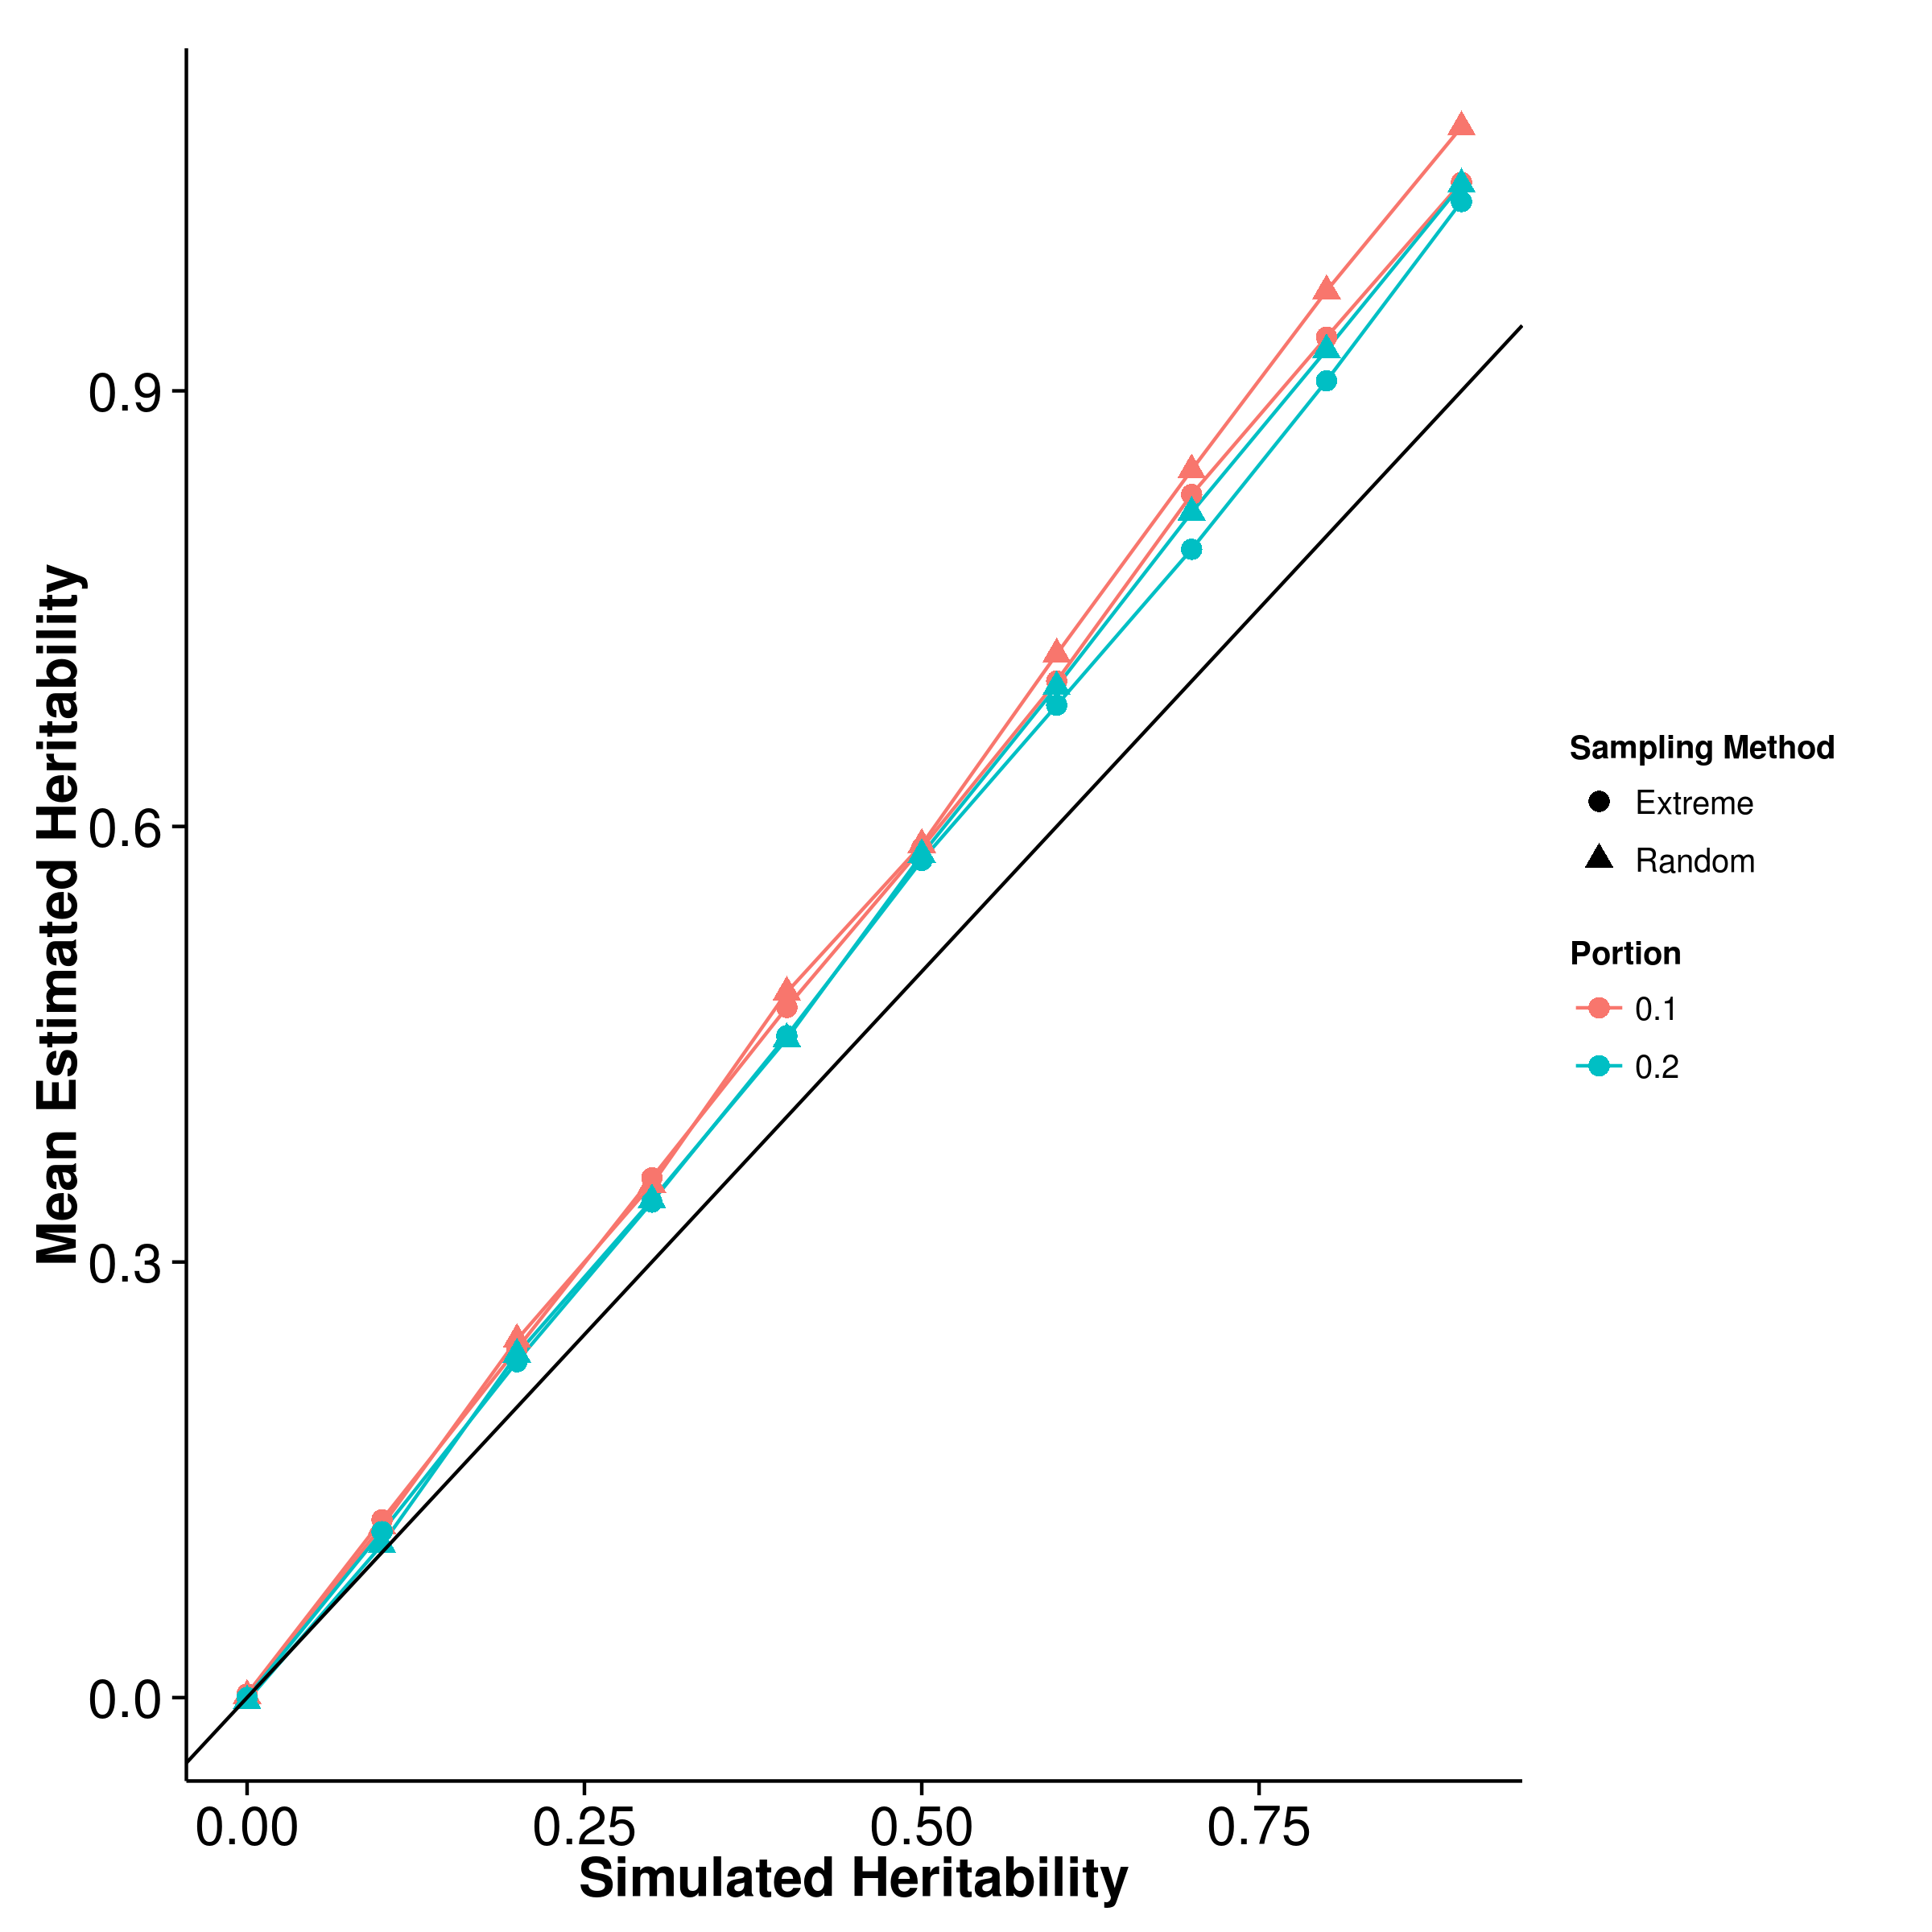
\includegraphics{figure/he_summary/pheno_extreme/shrek_extremeSelect_mean.png}}
				\label{fig:shrekExMean}
			}
			\subfloat[GCTA]{
				\scalebox{.4}{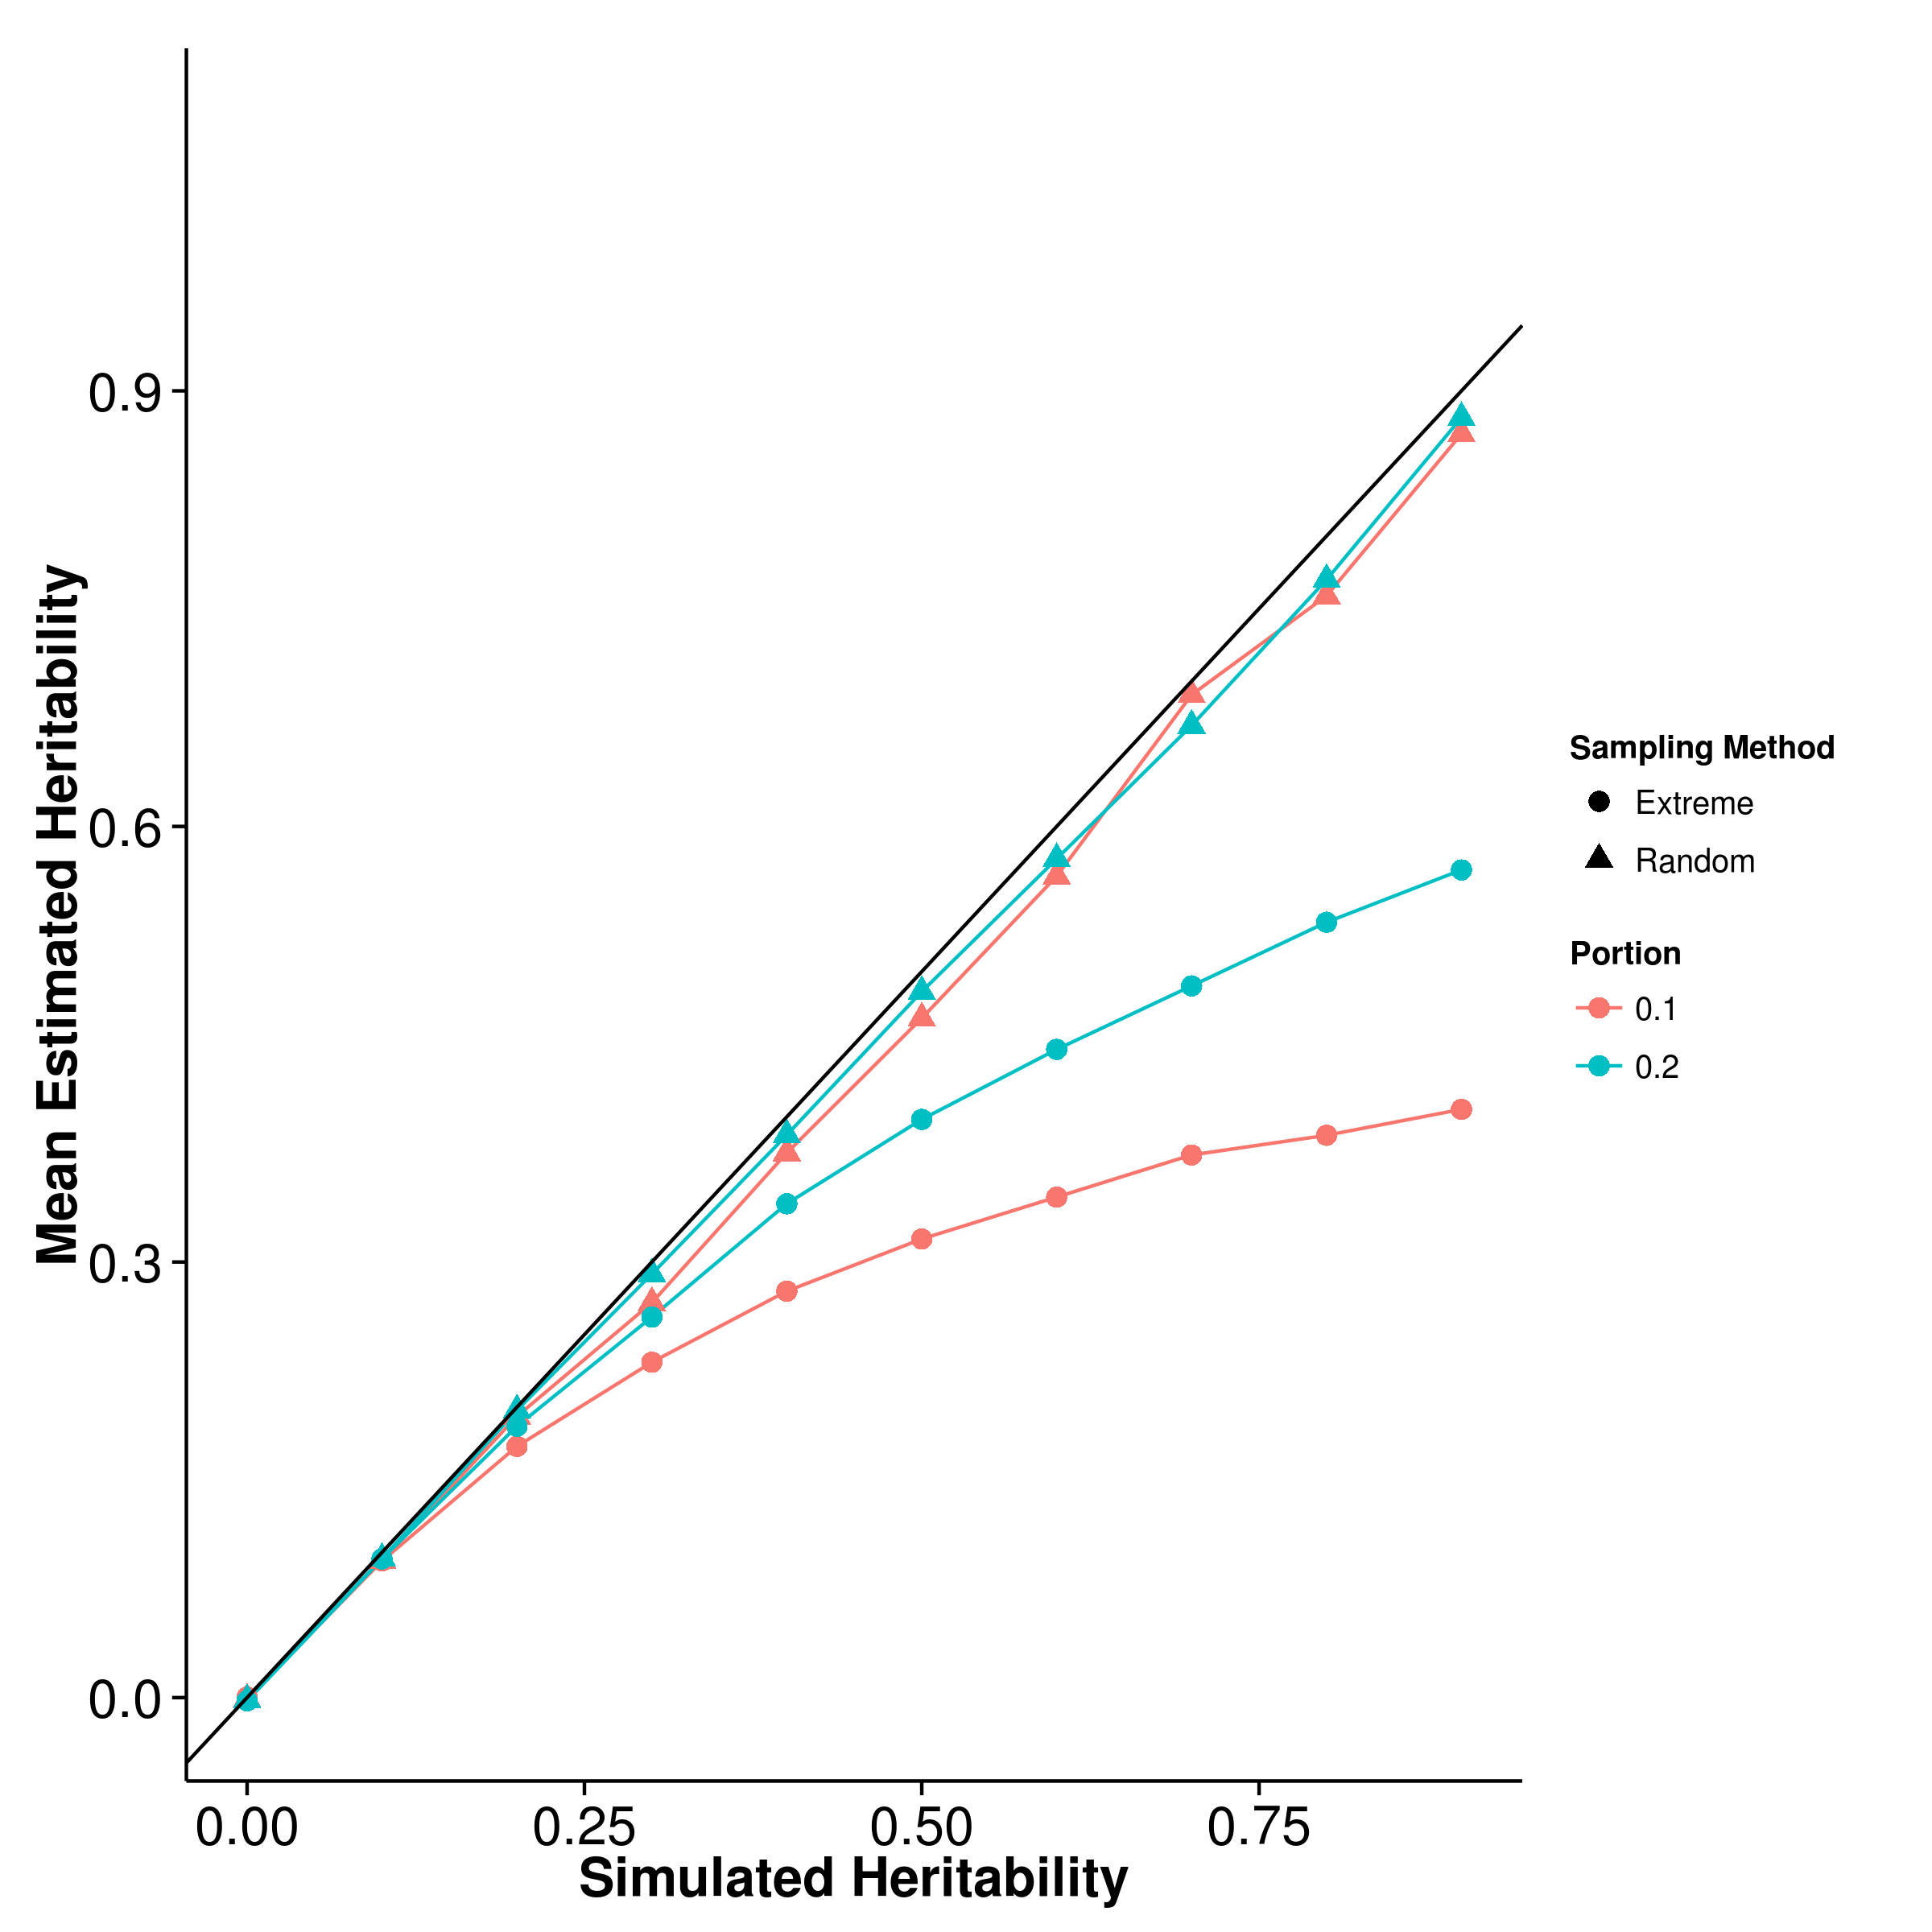
\includegraphics{figure/he_summary/pheno_extreme/gcta_extremeSelect_mean.png}}
				\label{fig:gctaExMean}
			}\\
			\subfloat[LDSC with fix intercept]{
				\scalebox{.4}{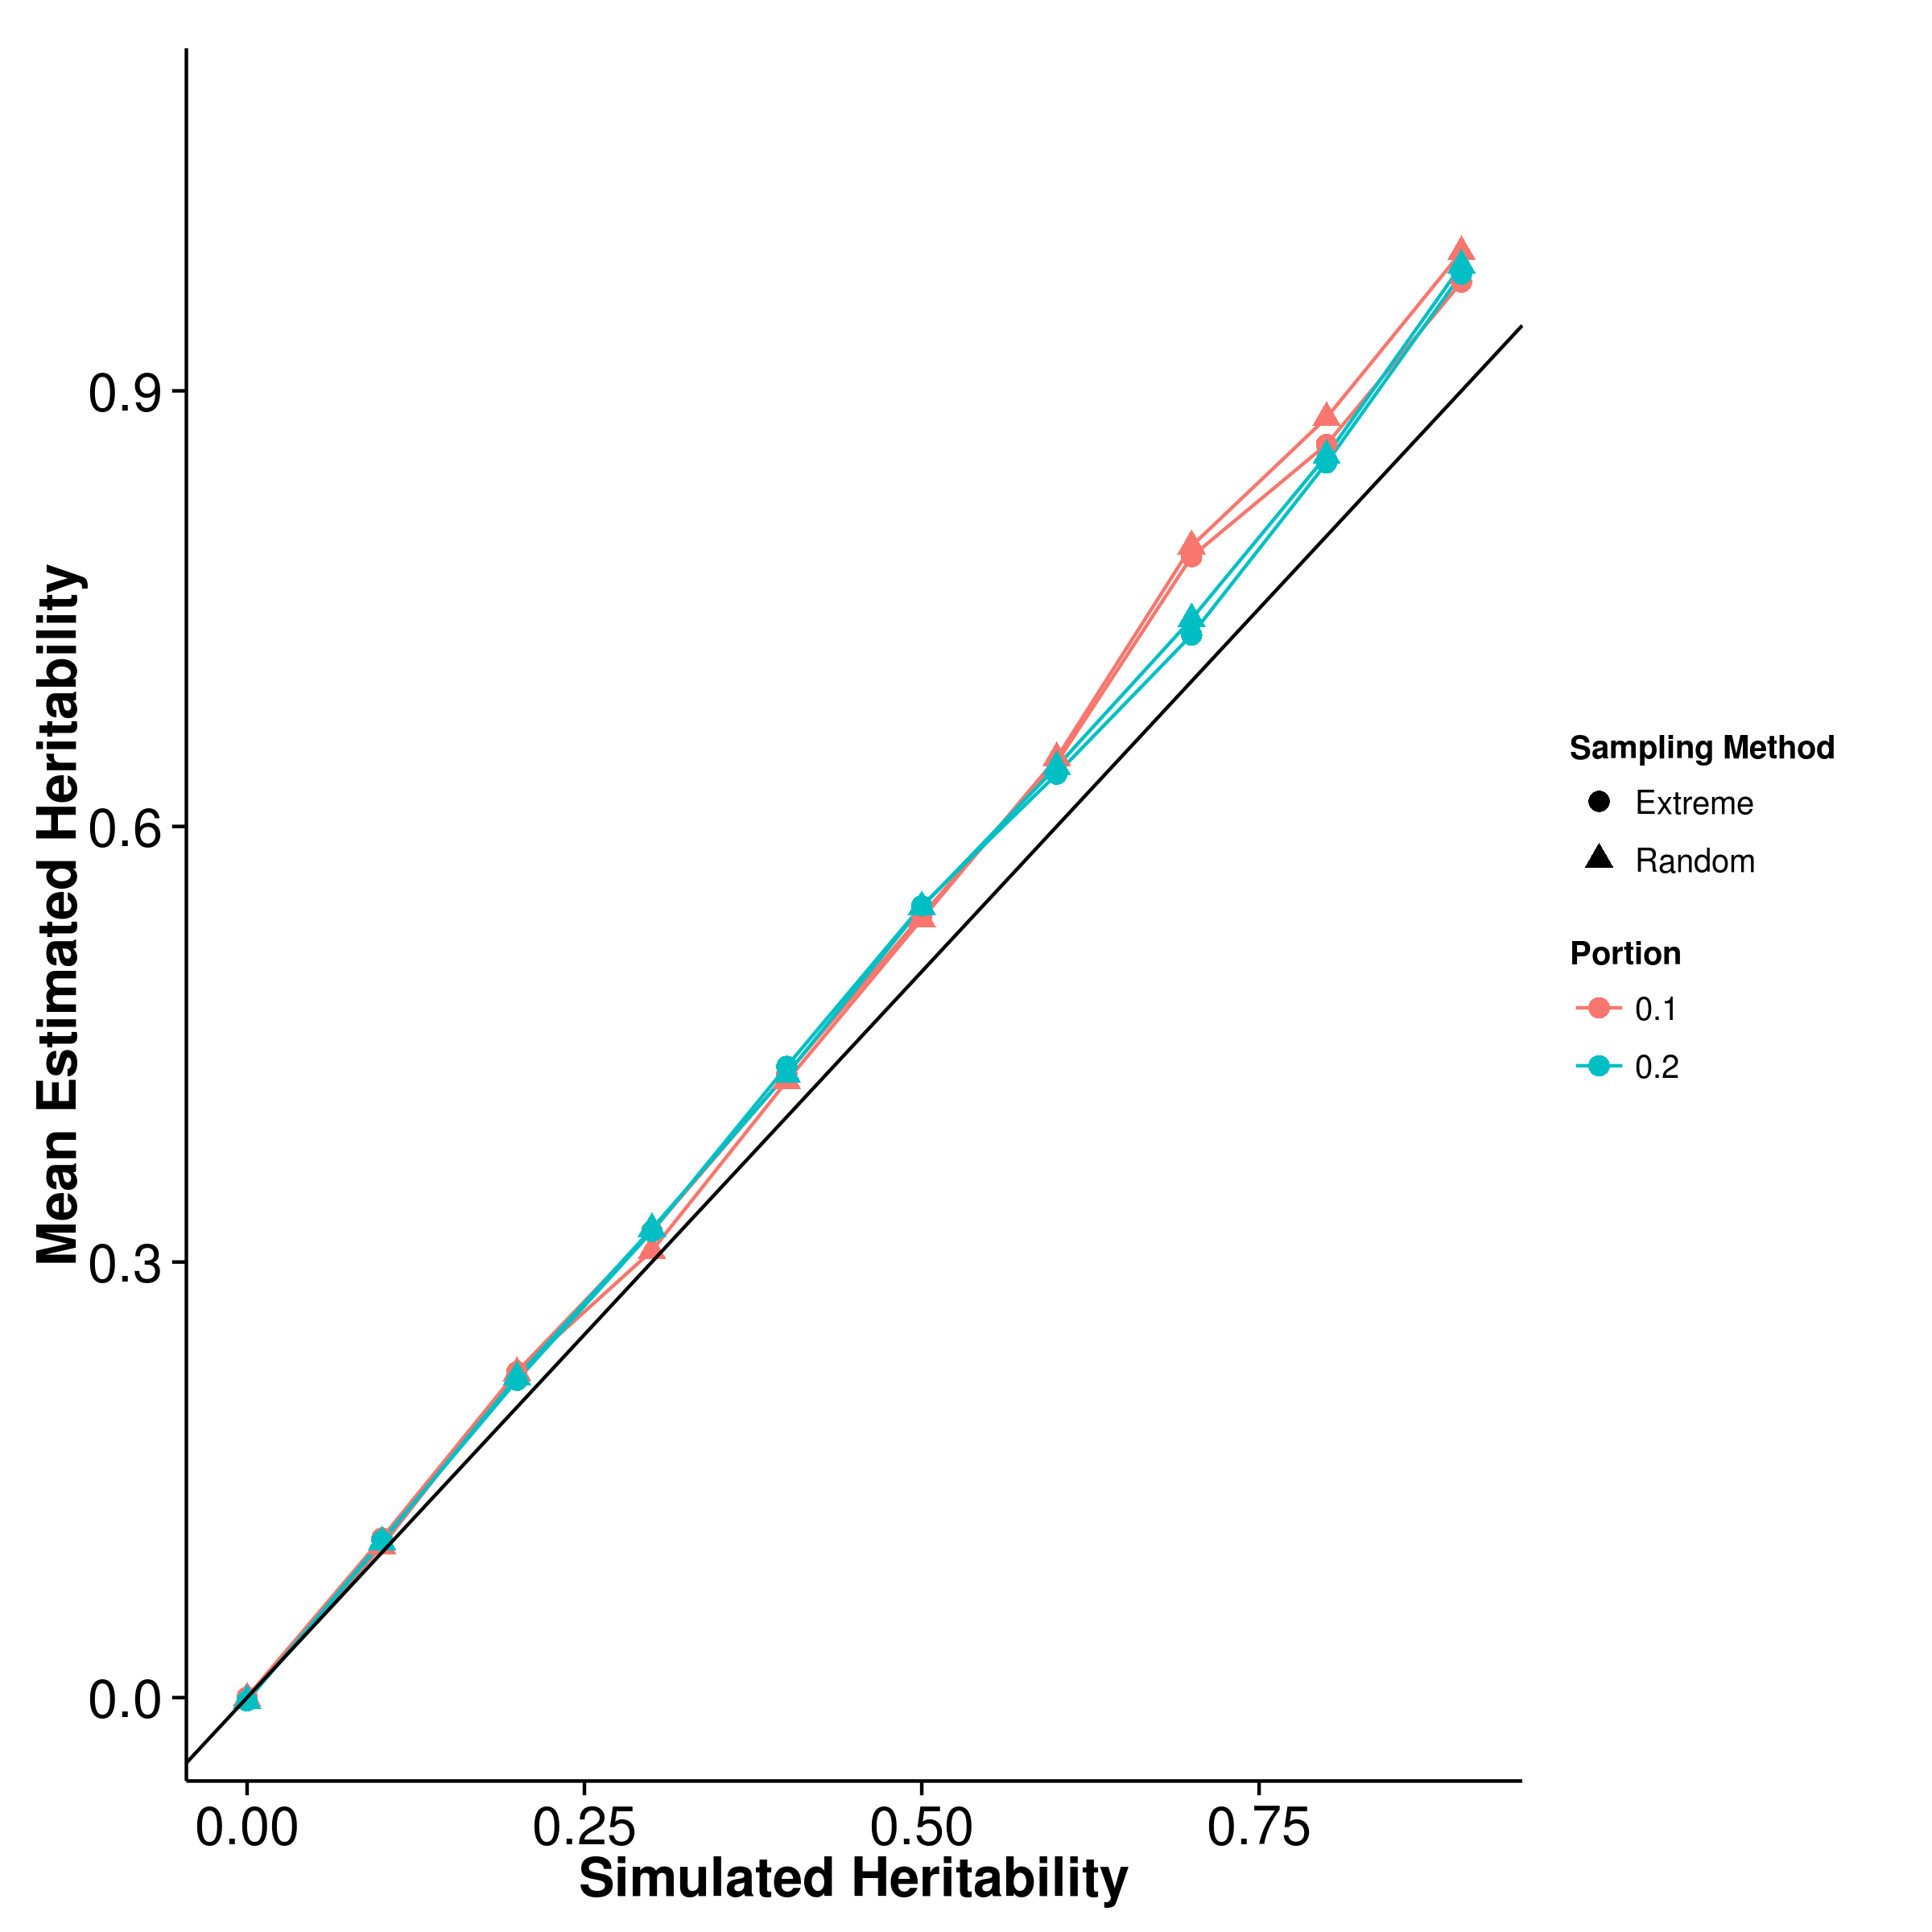
\includegraphics{figure/he_summary/pheno_extreme/ldsc_extremeSelect_mean.png}}
				\label{fig:ldscExMean}
			}
			\subfloat[LDSC with intercept estimation]{
				
				\scalebox{.4}{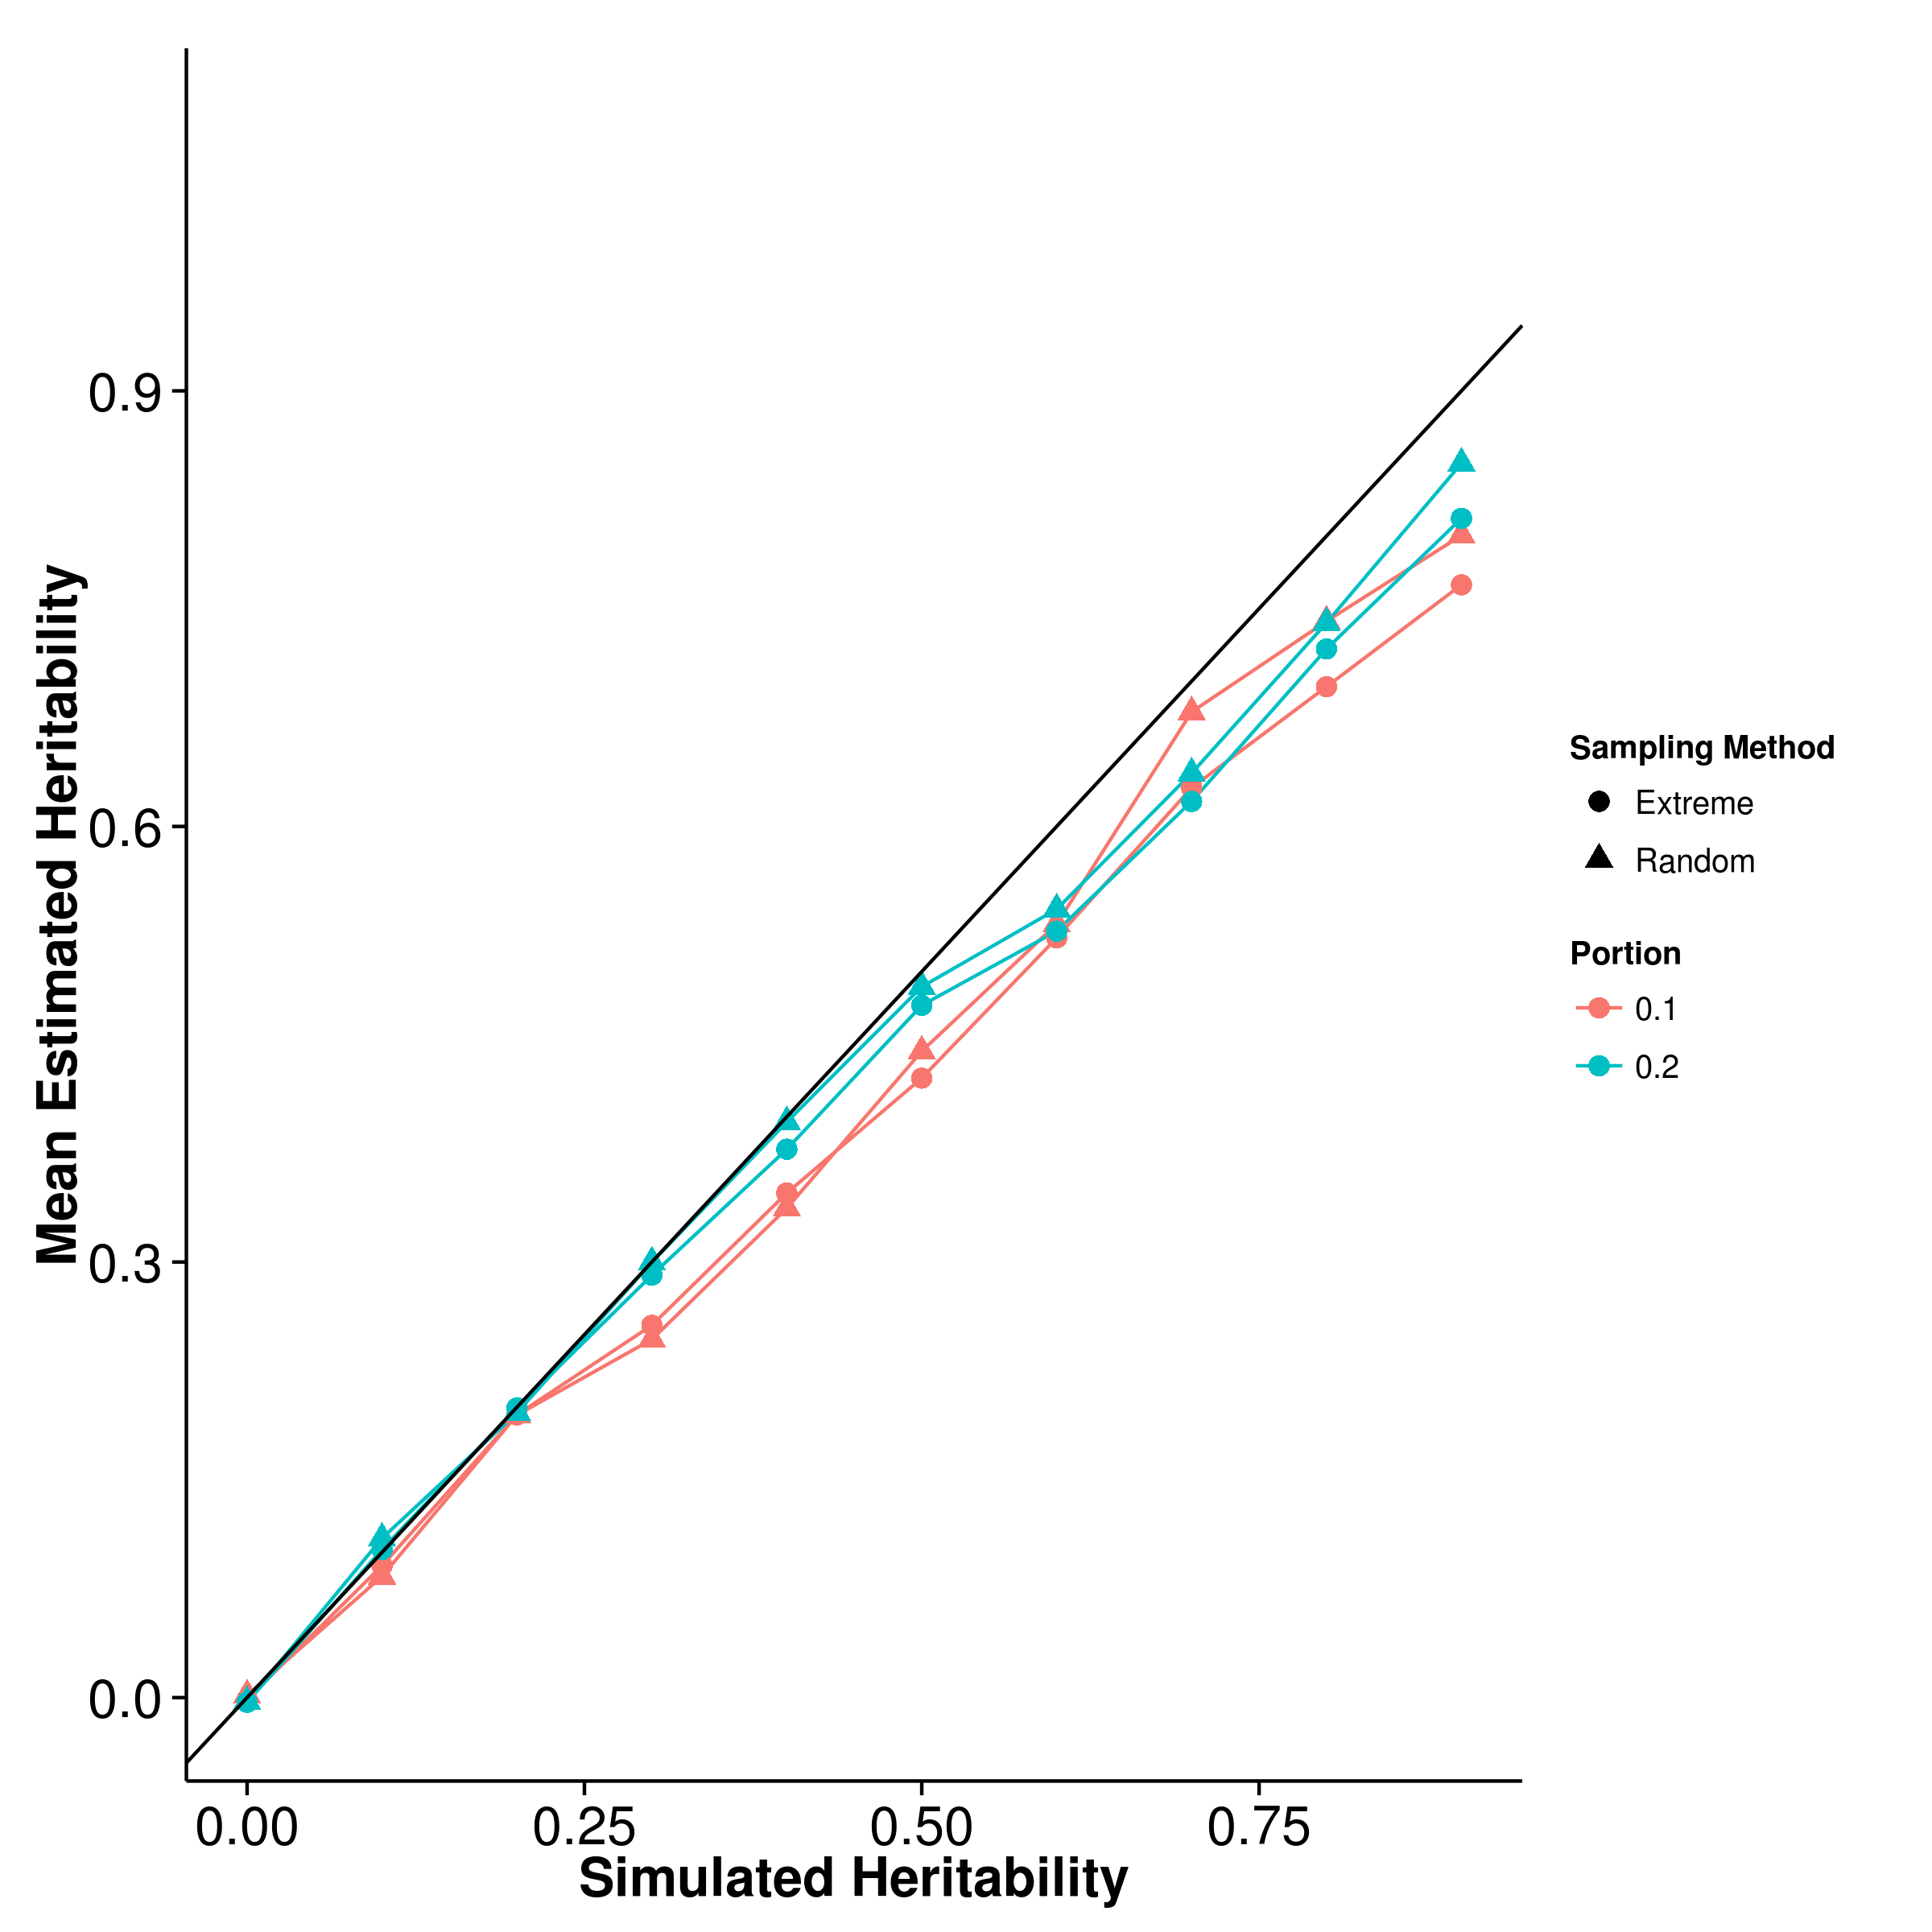
\includegraphics{figure/he_summary/pheno_extreme/ldscIn_extremeSelect_mean.png}}
				\label{fig:ldscInExMean}
			}
			\caption[Mean of Extreme Phenotype Selection Simulation Results]
			{Mean of results from extreme phenotype simulation.
				The performance of the algorithms when random sampling was performed were similar to what was observed in the quantitative trait simulation.
				However, when extreme phenotype was performed, a larger under estimation was observed for \gls{gcta} and it gets worst when the portion of sample selected decreases.
				On the other hand, the performance of \gls{shrek} and \gls{ldsc} under the extreme phenotype selection was similar to that from the random samplings.
				} 
			\label{fig:ExMean}
		\end{figure}
		
		\begin{figure}
			\centering
			\subfloat[SHREK]{
				\scalebox{.4}{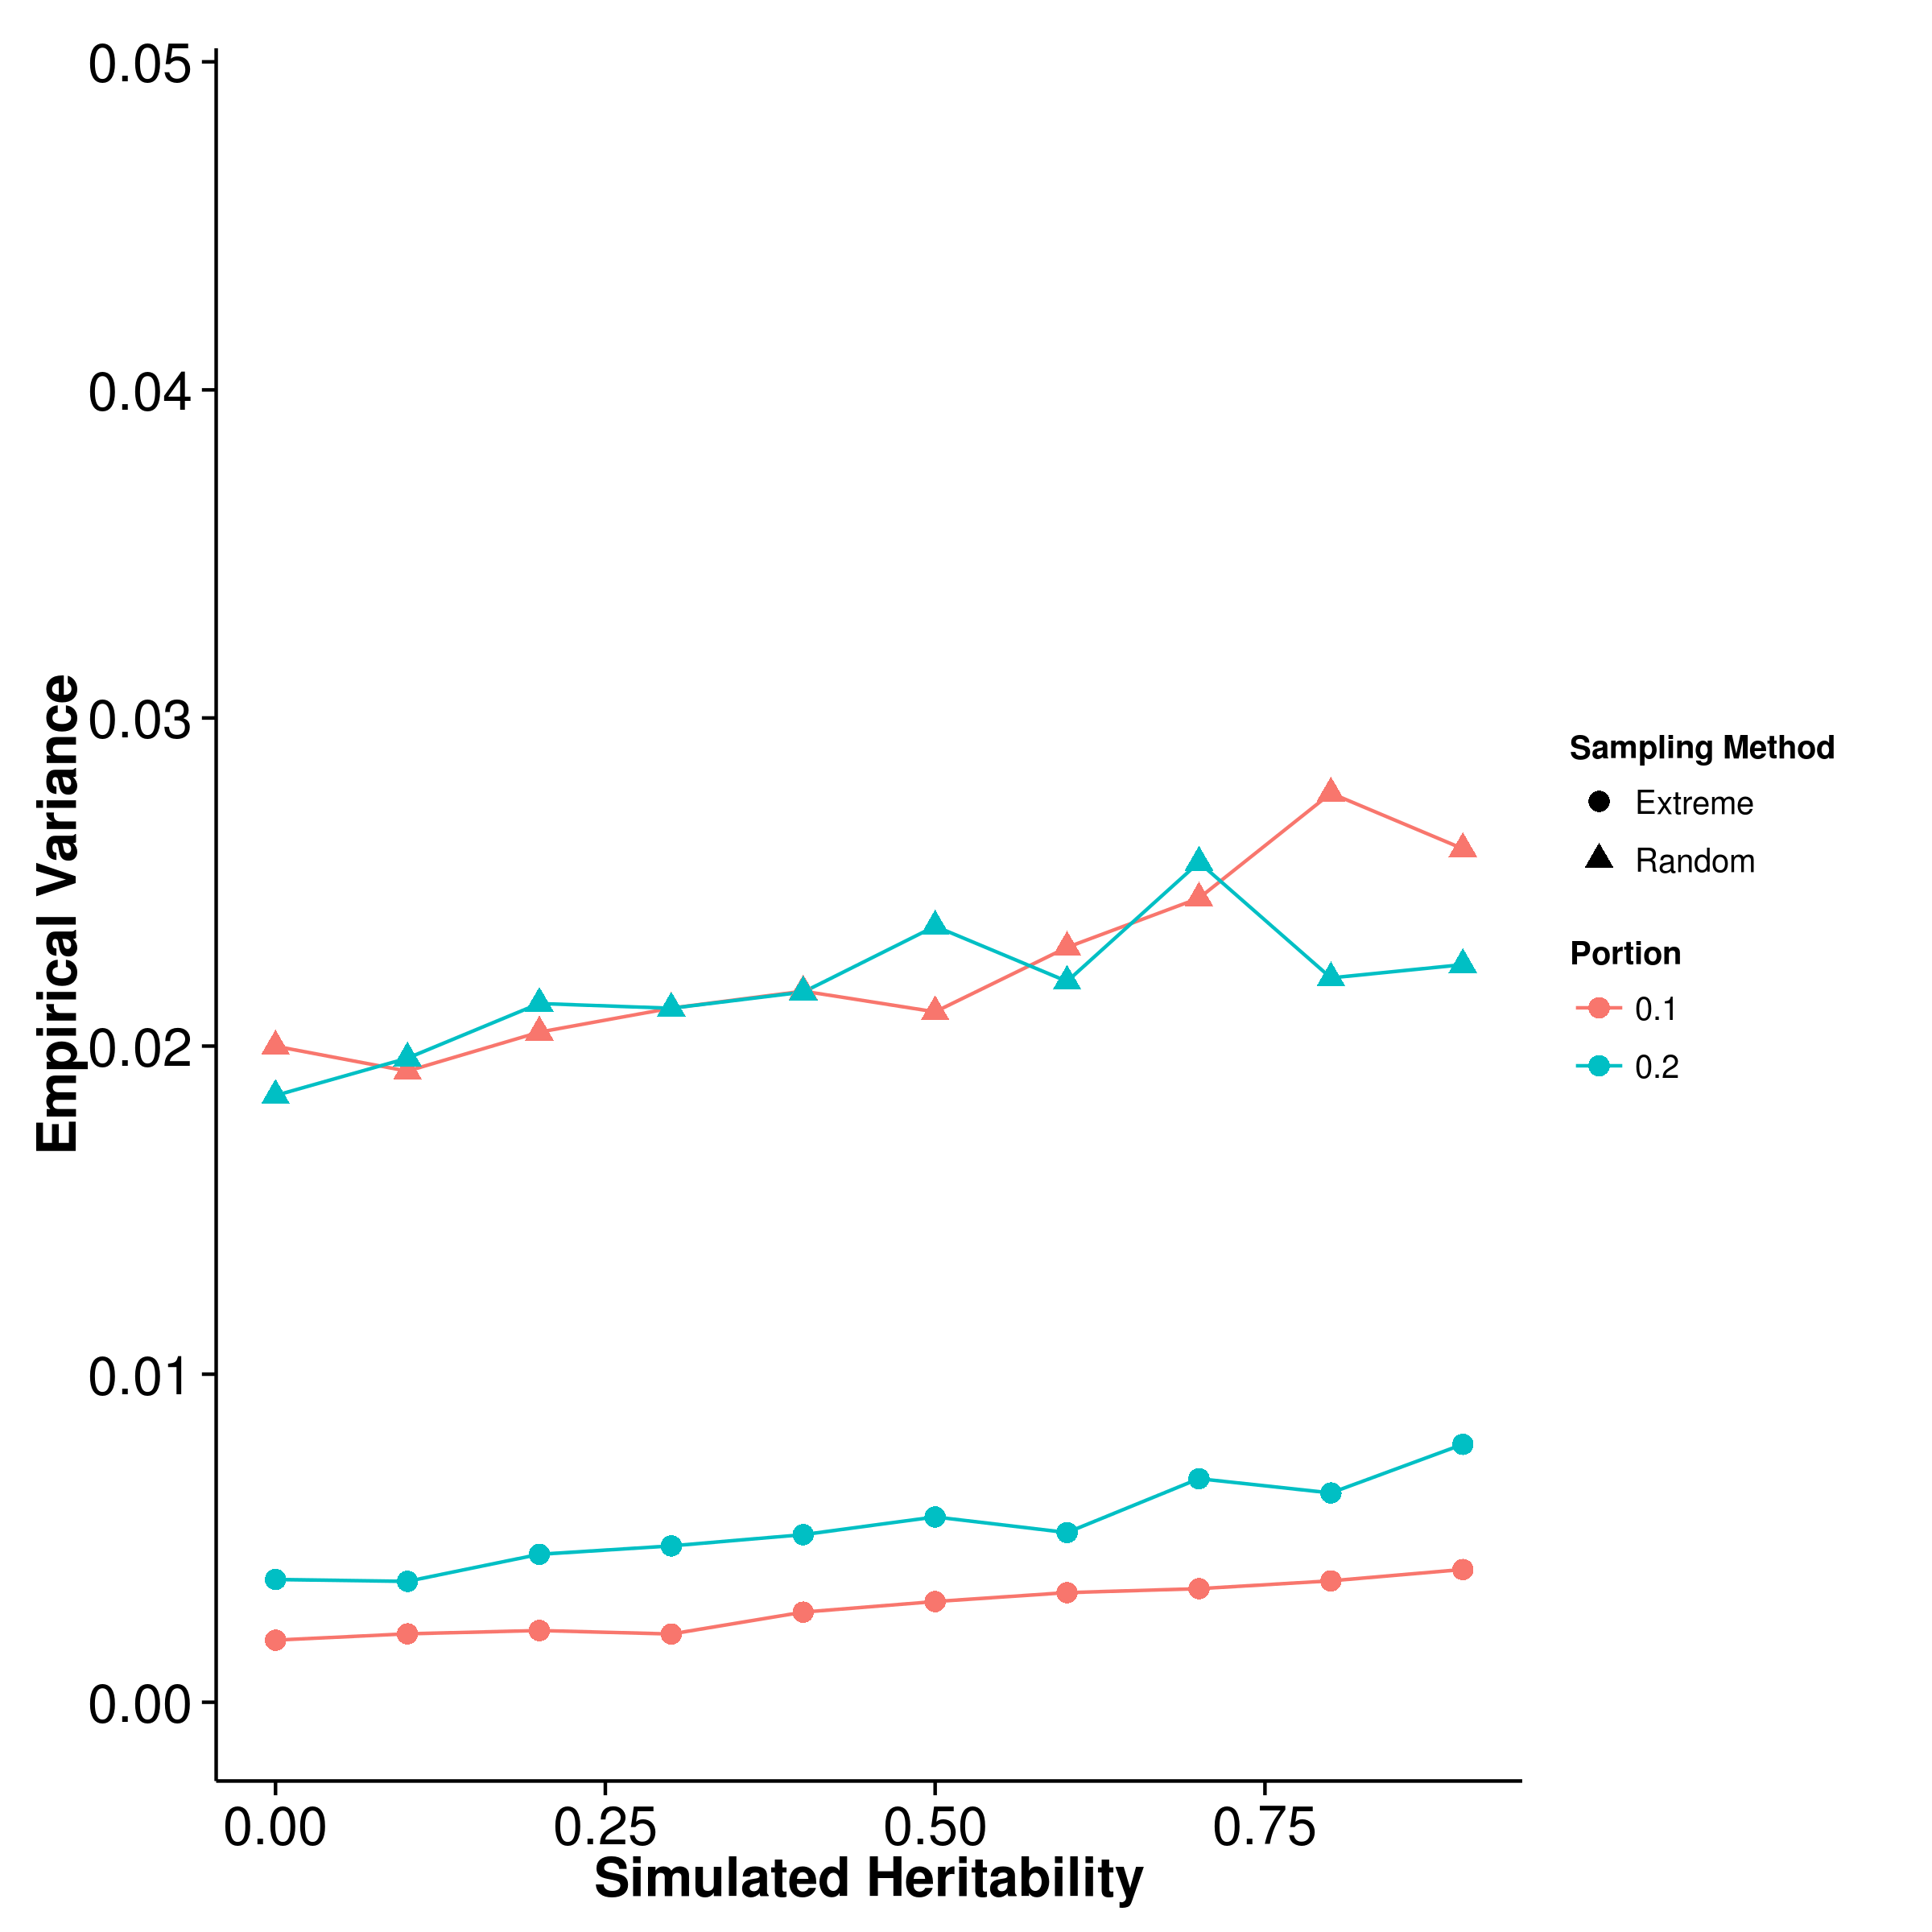
\includegraphics{figure/he_summary/pheno_extreme/shrek_extremeSelect_var.png}}
				\label{fig:shrekExVar}
			}
			\subfloat[GCTA]{
				\scalebox{.4}{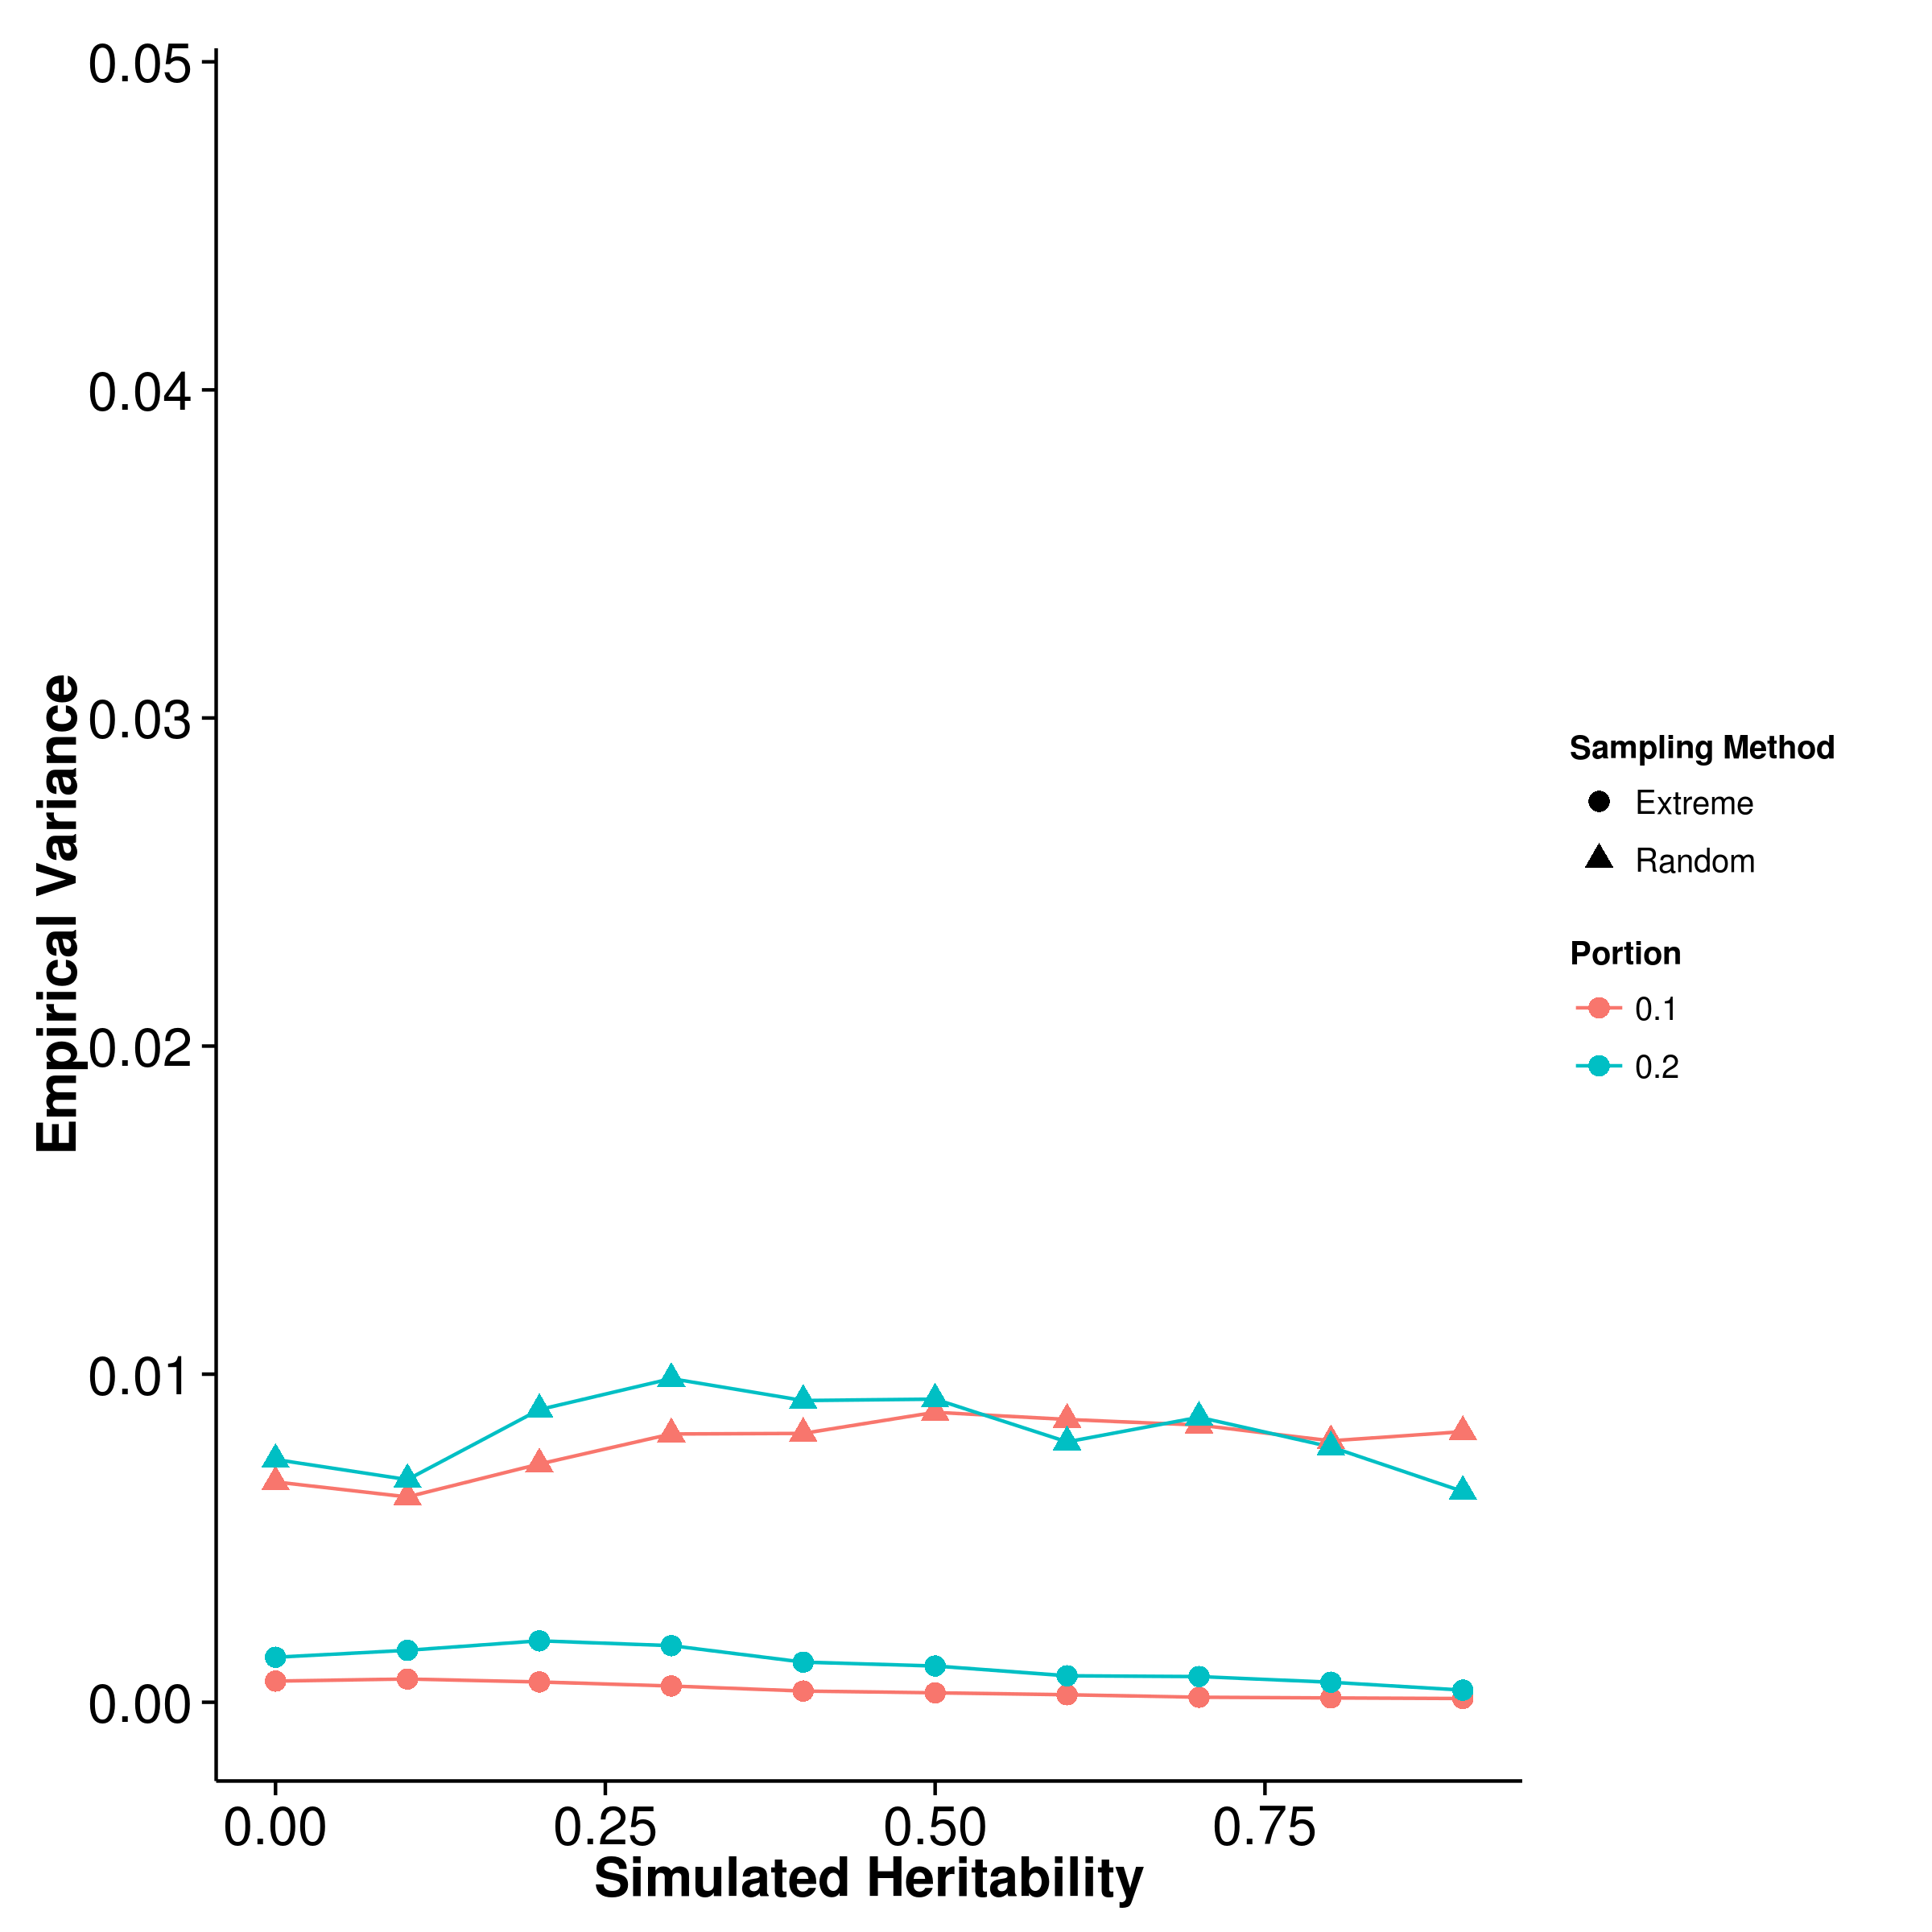
\includegraphics{figure/he_summary/pheno_extreme/gcta_extremeSelect_var.png}}
				\label{fig:gctaExVar}
			}\\
			\subfloat[LDSC with fix intercept]{
				\scalebox{.4}{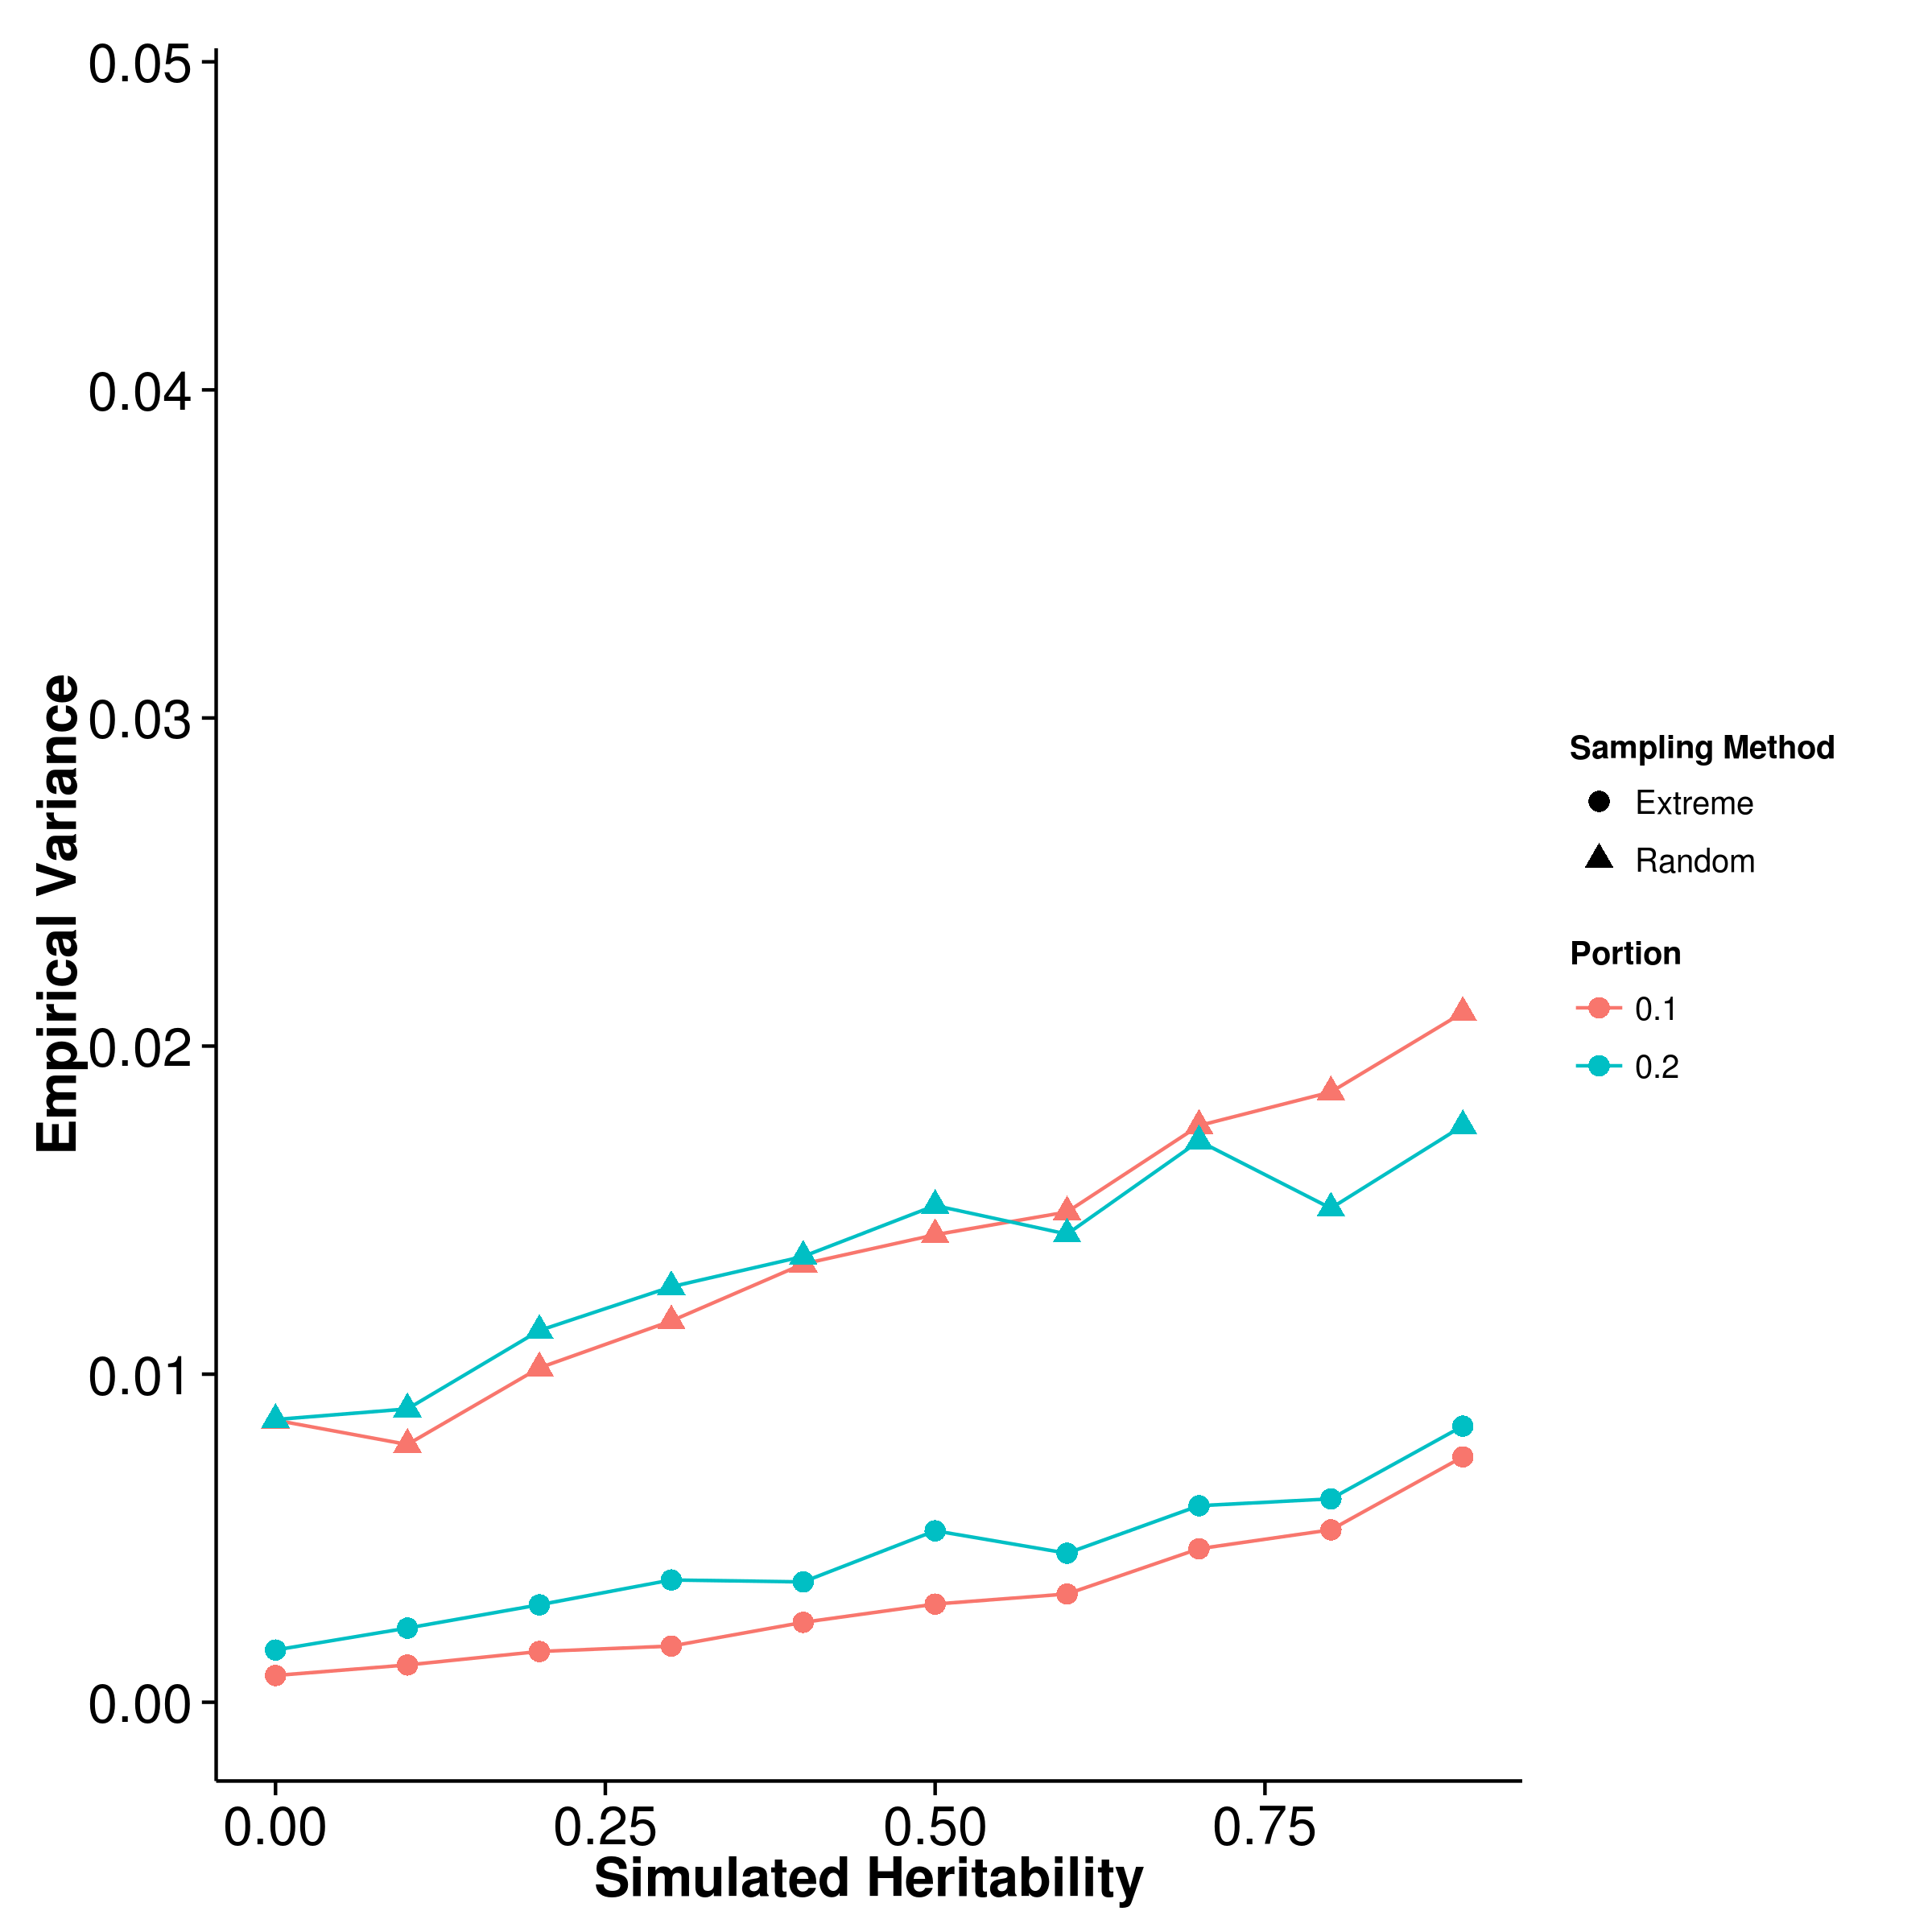
\includegraphics{figure/he_summary/pheno_extreme/ldsc_extremeSelect_var.png}}
				\label{fig:ldscEx}
			}
			\subfloat[LDSC with intercept estimation]{
				
				\scalebox{.4}{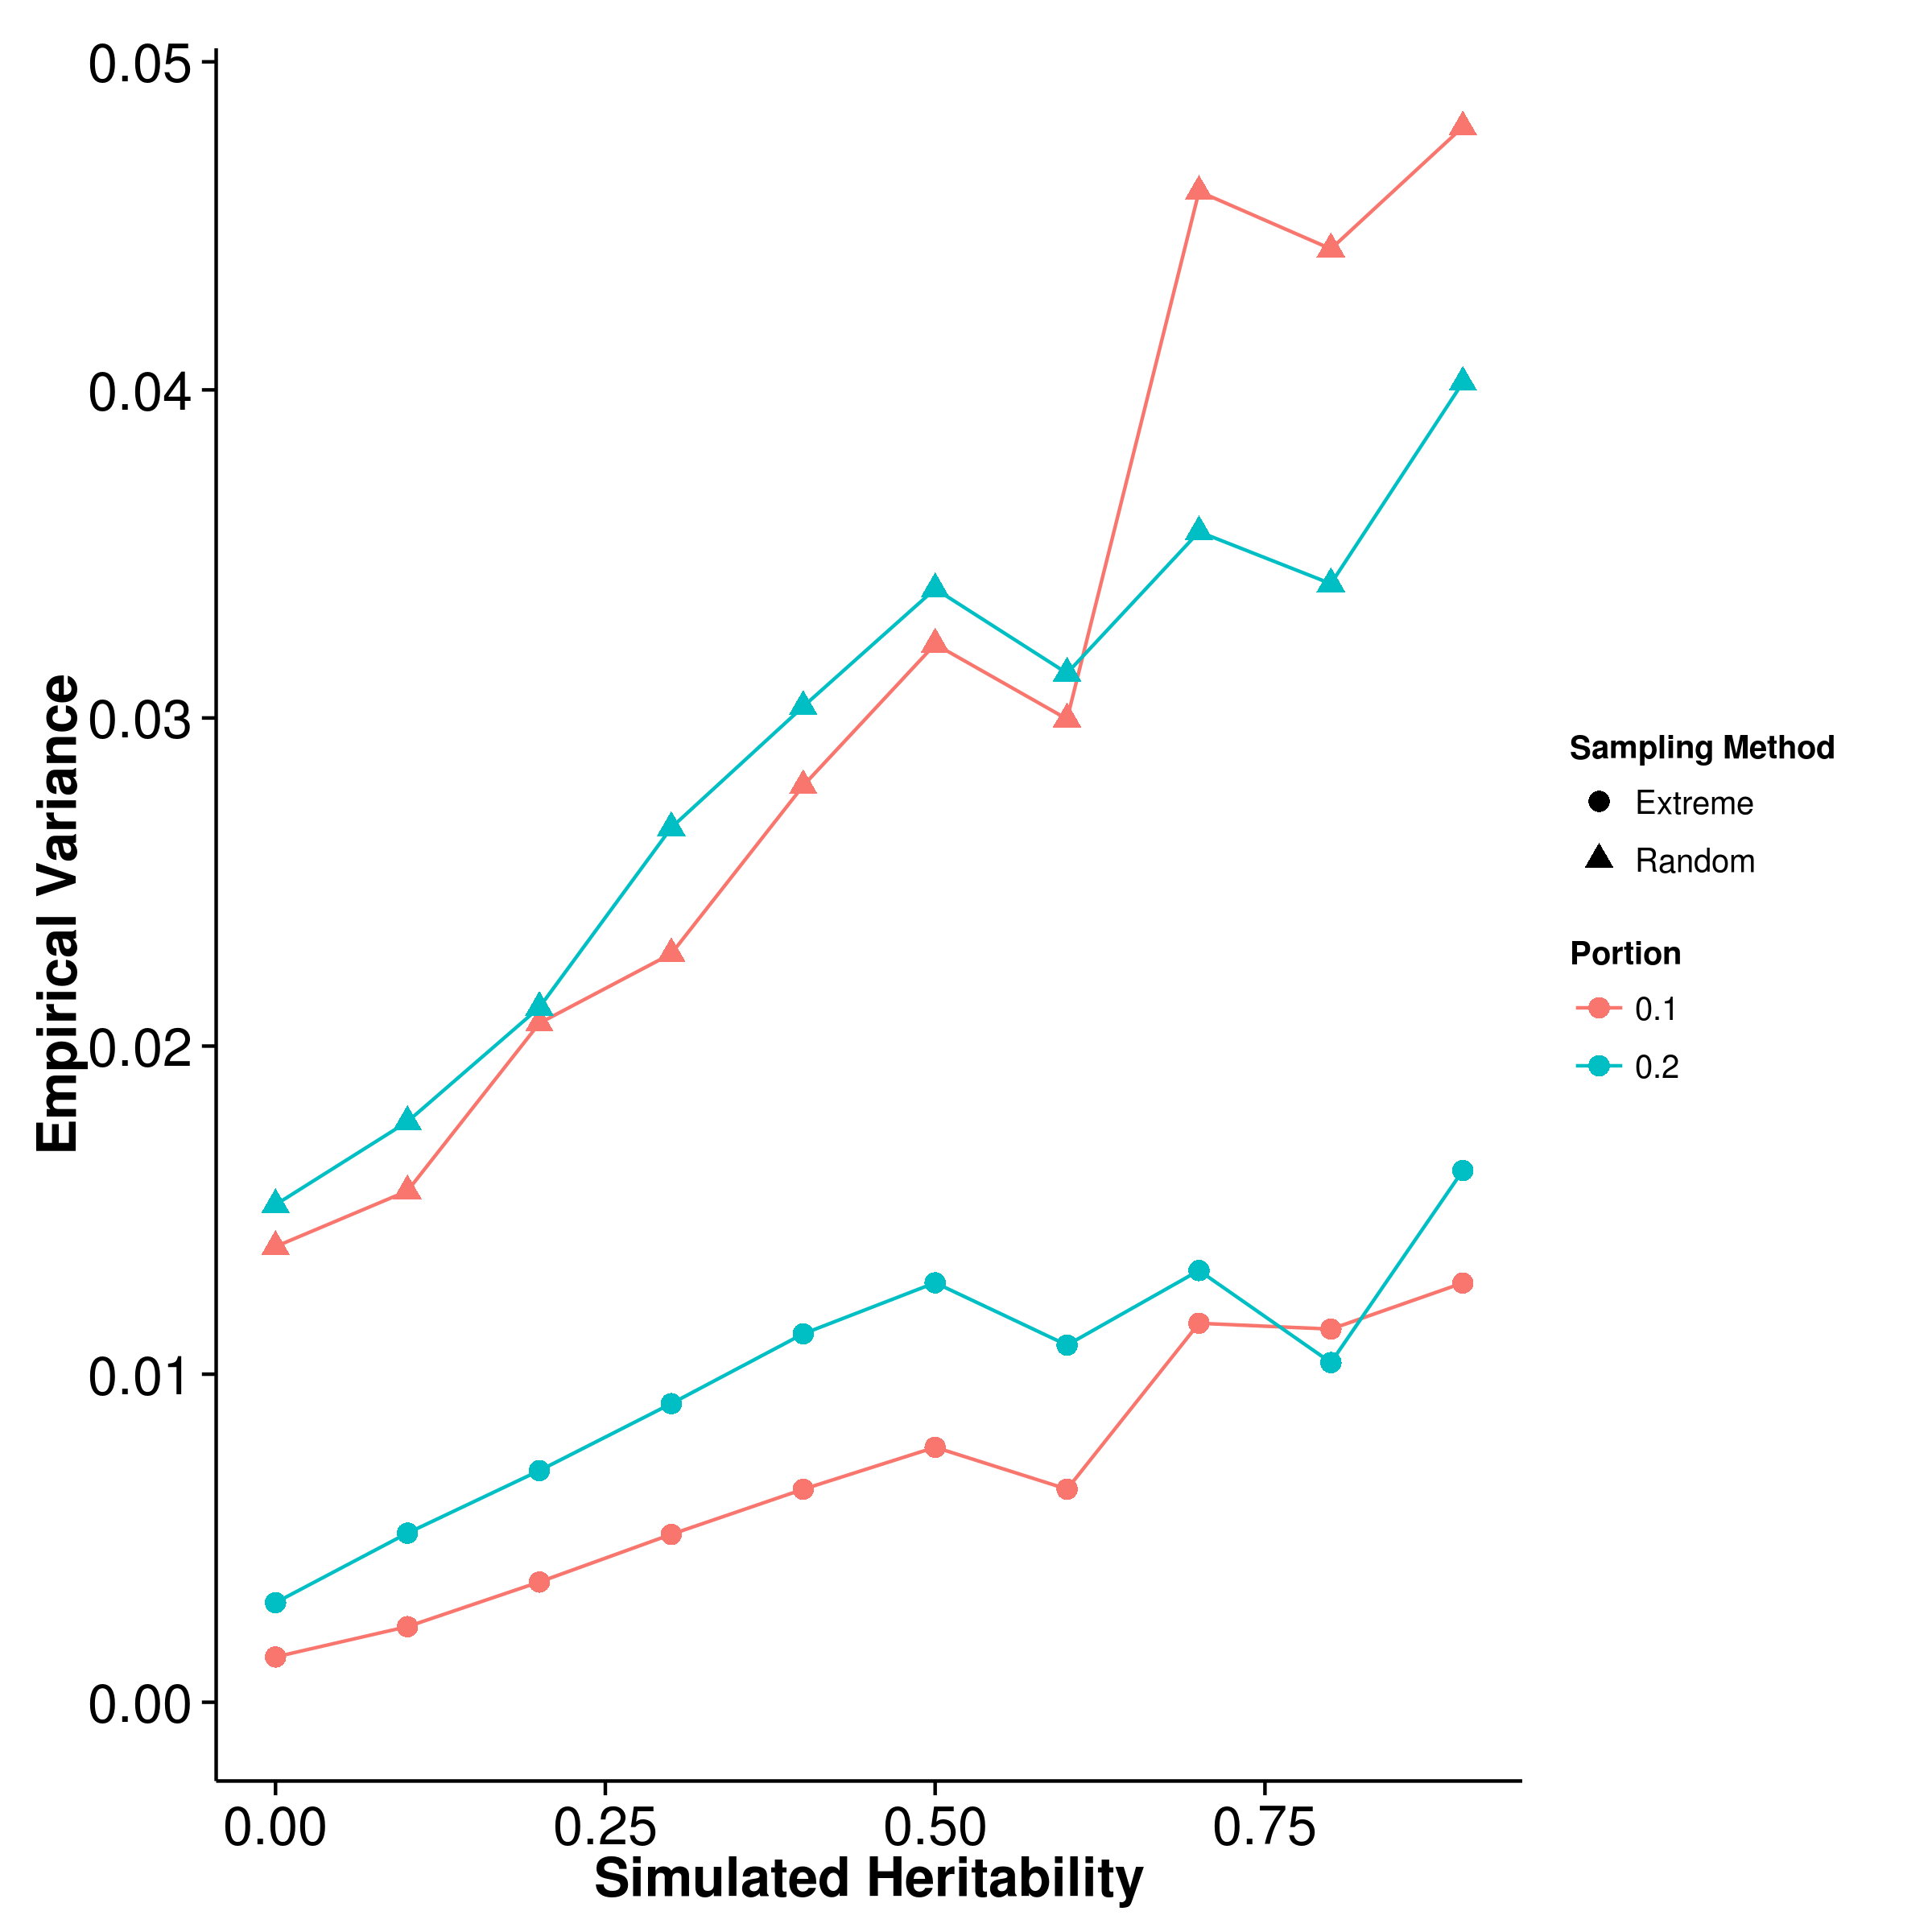
\includegraphics{figure/he_summary/pheno_extreme/ldscIn_extremeSelect_var.png}}
				\label{fig:ldscInExVar}
			}
			\caption[Variance of Extreme Phenotype Selection Simulation Results]
			{Variance of results from extreme phenotype simulation.
				It is obvious that when the extreme phenotype selection was performed, the empirical variance of all the algorithm decreases and is much smaller than the empirical variance of the estimation when random sampling was performed.
				We also compared the empirical variance of random sampling with those from quantitative trait simulation with 100 causal \glspl{SNP} and they are highly similar. 
			} 
			\label{fig:ExVar}
		\end{figure}
		
		
		\begin{figure}
			\centering
			\subfloat[SHREK]{
				\scalebox{.4}{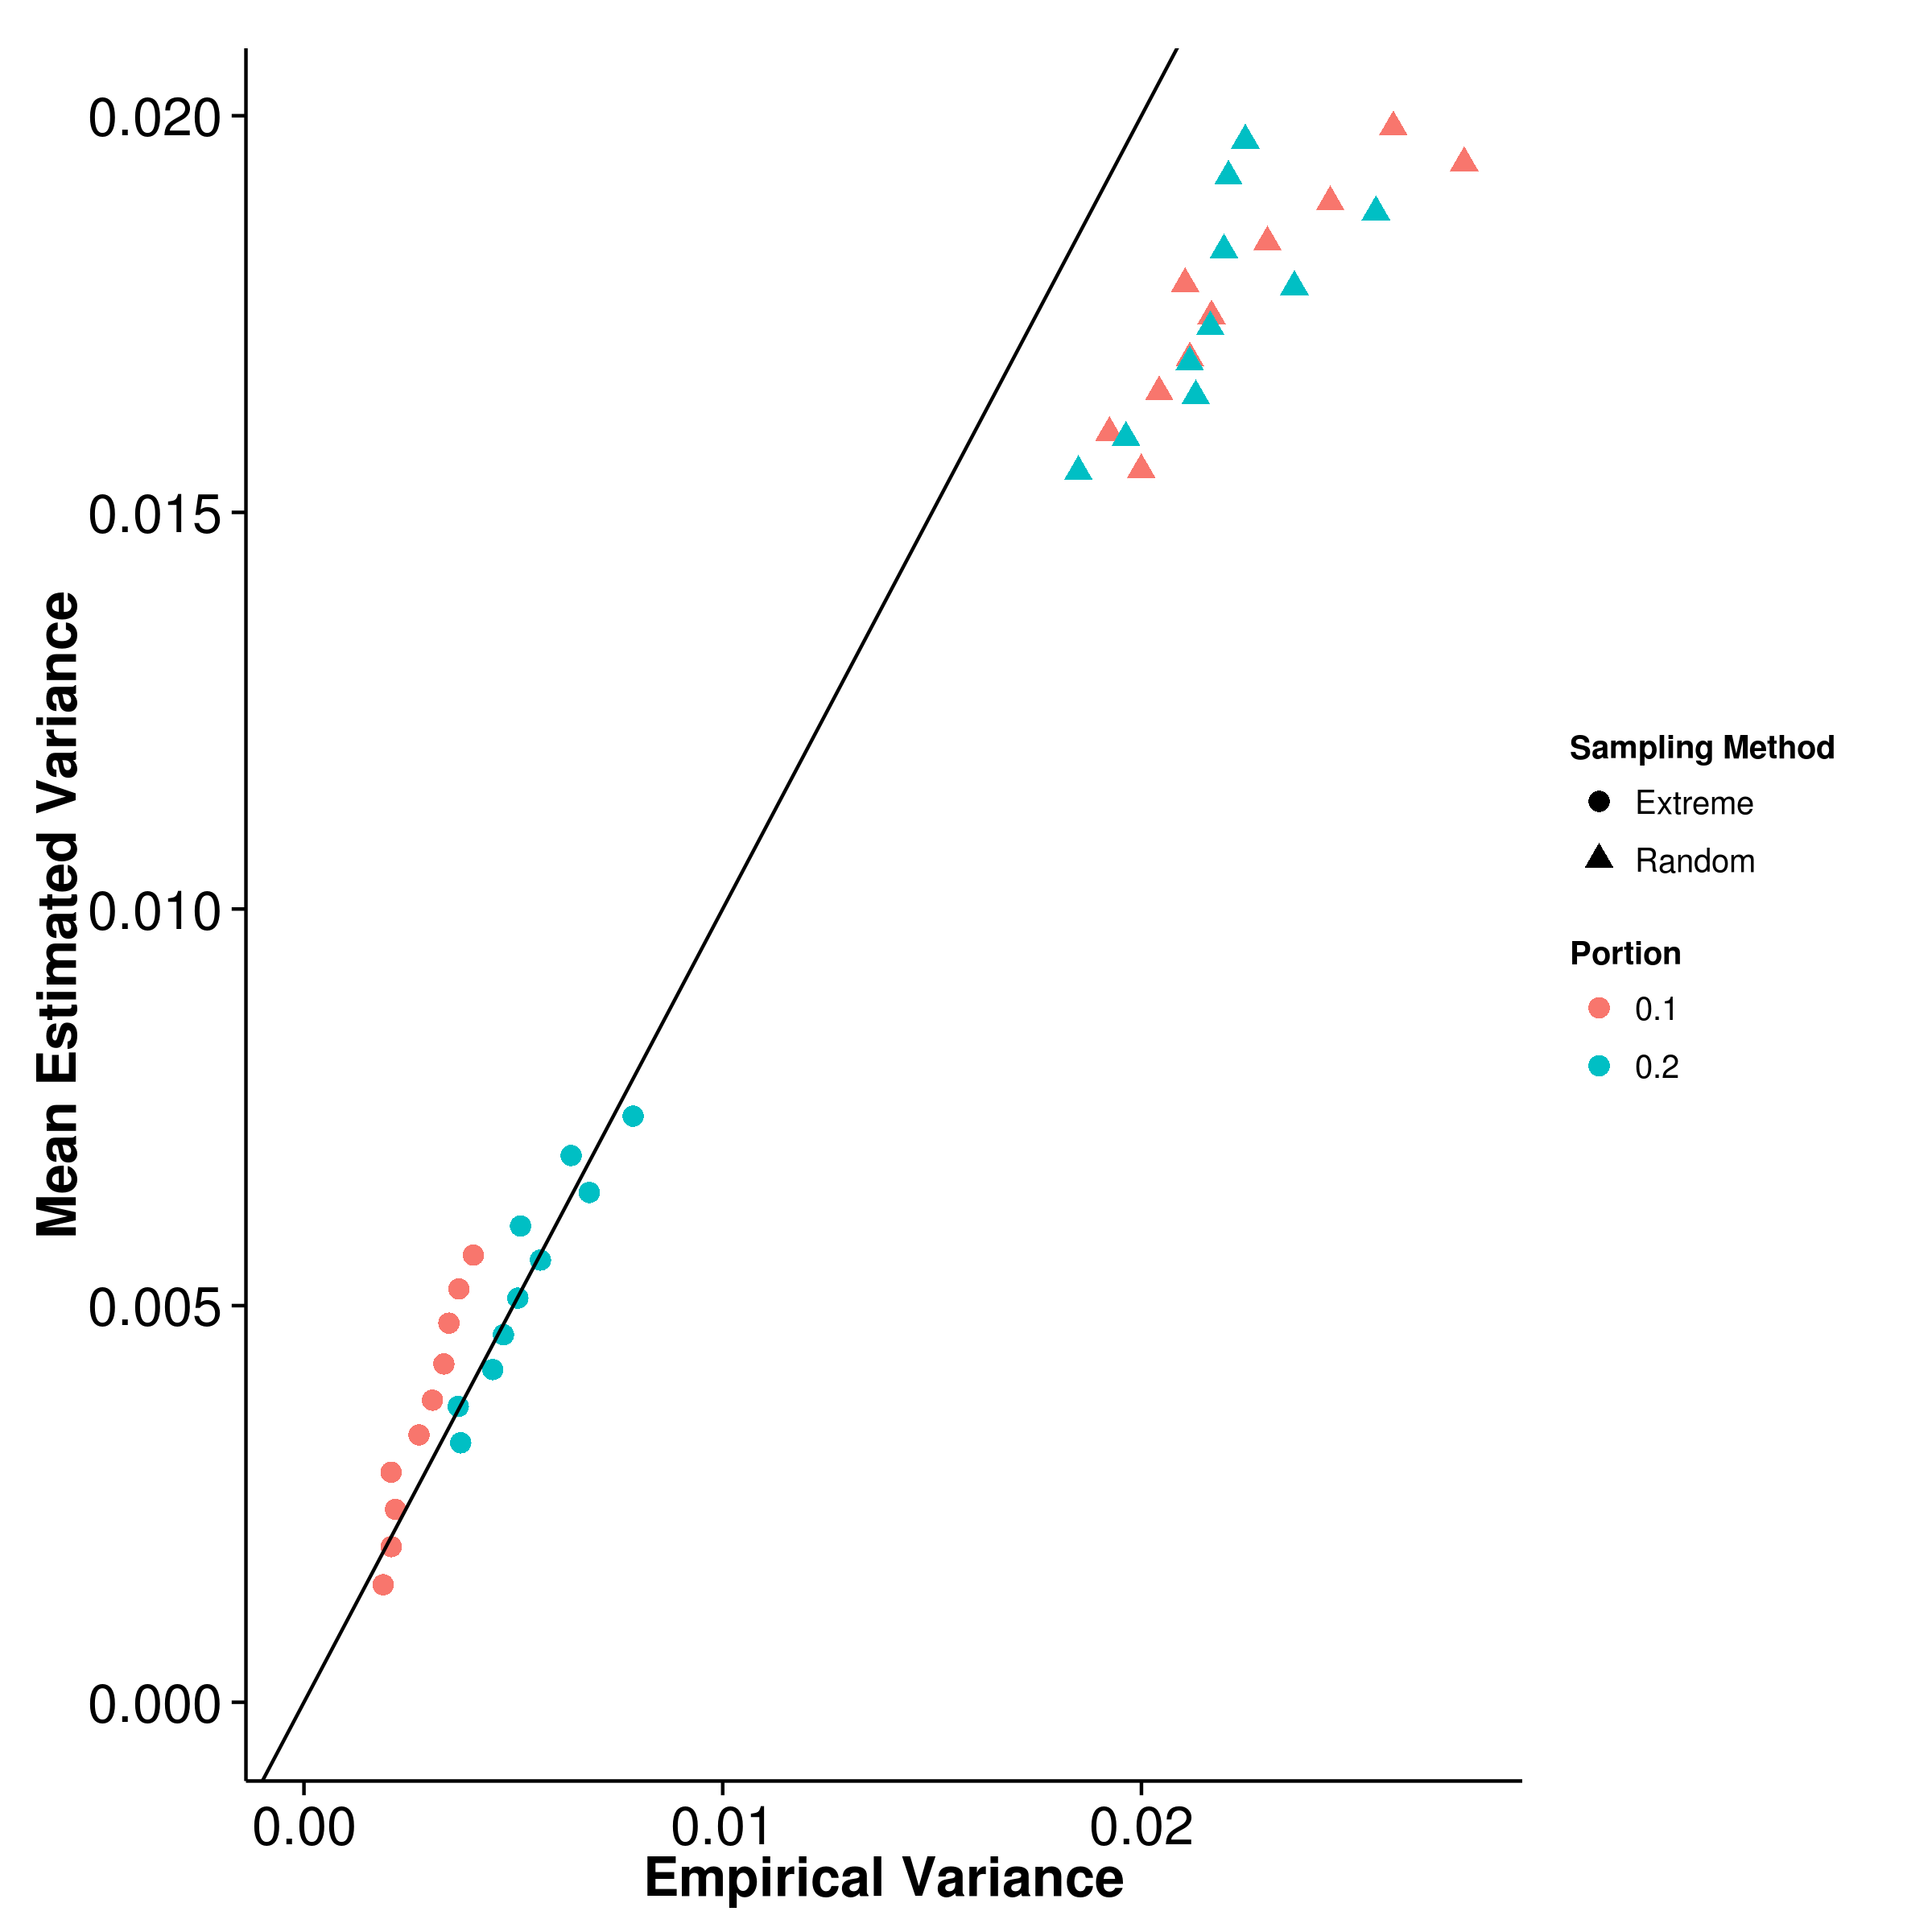
\includegraphics{figure/he_summary/pheno_extreme/shrek_extremeSelect_varCom.png}}
				\label{fig:shrekExVarCom}
			}
			\subfloat[GCTA]{
				\scalebox{.4}{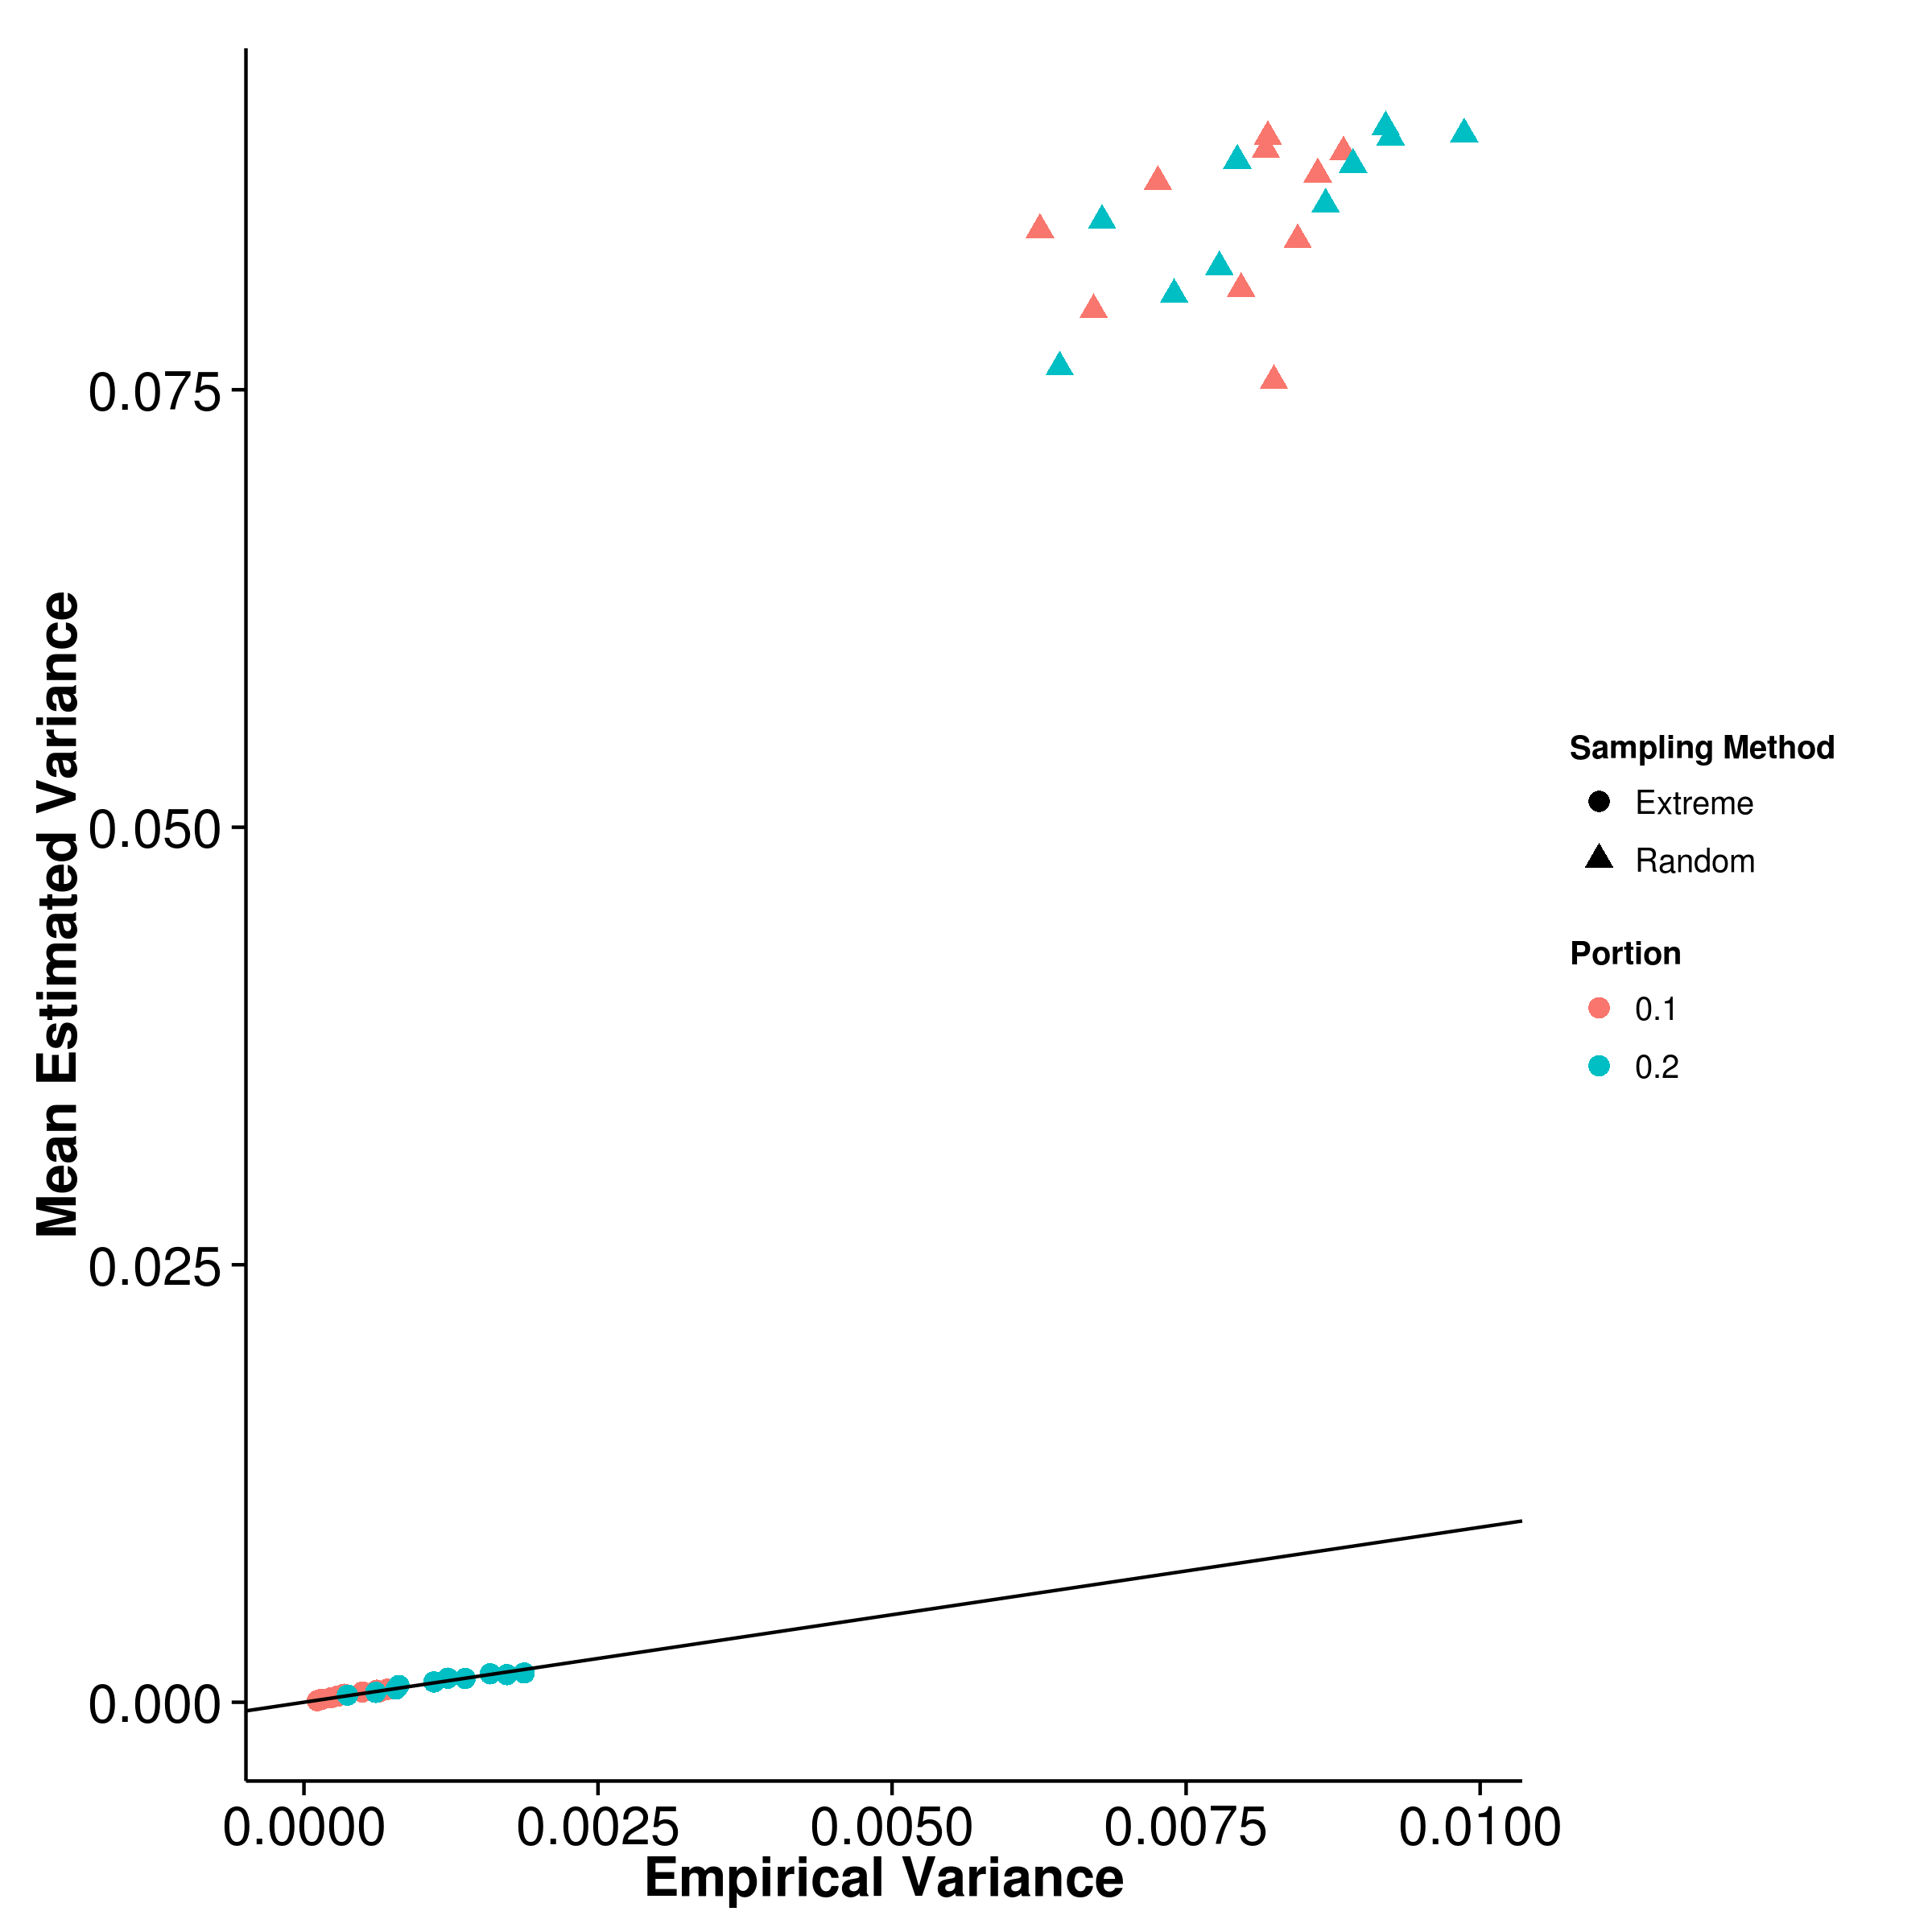
\includegraphics{figure/he_summary/pheno_extreme/gcta_extremeSelect_varCom.png}}
				\label{fig:gctaExVarCom}
			}\\
			\subfloat[LDSC with fix intercept]{
				\scalebox{.4}{\includegraphics{figure/he_summary/pheno_extreme/ldsc_extremeSelect_varCom.png}}
				\label{fig:ldscExVarCom}
			}
			\subfloat[LDSC with intercept estimation]{
				
				\scalebox{.4}{\includegraphics{figure/he_summary/pheno_extreme/ldscIn_extremeSelect_varCom.png}}
				\label{fig:ldscInExVarCom}
			}
			\caption[Estimation of Variance in Extreme Phenotype Selection]
			{Estimated variance of results from extreme phenotype selection when compared to empirical variance.
				Surprisingly, except for \gls{shrek}, the estimated variance from \gls{ldsc} and \gls{gcta} under the random sampling condition was much higher than the empirical variance. 
				It is much different from the estimated variance from the quantitative trait simulation and further investigations are required to understand this discrepancy.
				} 
			\label{fig:ExVarCom}
		\end{figure}
		Sometimes, when budget is limited, it is not possible to include all samples in the final \gls{GWAS}. 
		By using appropriate sampling strategy, such as that of extreme phenotype sampling \citep{Peloso2015}, one can increase the power of the association study.
		Here we perform simulations using extreme phenotype sampling and study the effect of this selection on the performance of heritability estimations.
		The random sampling procedure were also performed in our simulation such that a clear comparison can be made between the power of extreme phenotype sampling and the traditional random sampling.
		
		From the graph (\cref{fig:ExMean}), it was observed that performance of \gls{shrek} and \gls{ldsc} were similar to what was observed in the quantitative trait simulation, where when the random sampling strategy were used, higher estimation were usually obtained. 
		Interestingly, \gls{gcta} performs poorly when extreme phenotype sampling was performed where as the portion of sample decreases, the bias of the estimates increases (\cref{fig:gctaExMean}).
		
		When comparing the empirical variance, the random sampling strategy consistently result in  larger variance when compared to extreme phenotype sampling strategy (\cref{tab:ratioEx}).
		The \gls{mse} from extreme phenotype sampling can be as much as 4 fold smaller for \gls{shrek} and \gls{ldsc} when compared to random sampling.
		
		Strangely, although the empirical variance under the random sampling strategy is the same as what was observed in the quantitative trait simulation, there is a large discrepancy in the estimated variance where a ten fold overestimation was observed for \gls{ldsc} and \gls{gcta} (\cref{fig:ExVarCom}). 
		More surprisingly, \gls{shrek} was unaffected. 
		We are uncertain of the origin of such problem and further investigation is required.
		
		
		\begin{table}
			\centering
			\begin{tabular}{rrrrrrrrr}
				\toprule
				\multirow{2}[4]{*}{Portion} & \multicolumn{2}{c}{Shrek} & \multicolumn{2}{c}{LDSC} & \multicolumn{2}{c}{LDSC-In} & \multicolumn{2}{c}{GCTA} \\
				& Extreme & Rand & Extreme & Rand & Extreme & Rand & Extreme & Rand\\
				\midrule
				0.1   & 0.0113 & 0.0341 & 0.00537 & 0.0167 & 0.0119 & 0.0329 & 0.0644 & 0.00849 \\
				0.2   & 0.0109 & 0.0290 & 0.00599 & 0.0152 & 0.0126 & 0.0299 & 0.0274 & 0.00852 \\
				\bottomrule
			\end{tabular}
			\caption[Comparing the MSE of Extreme Phenotype Sampling and Random Sampling]{
				Here, we compared the \gls{mse} of random sampling (Rand) against the \gls{mse} of Extreme phenotype sampling (Extreme). 
				With the exception of \gls{gcta}, the extreme phenotype selection generally produce a smaller \gls{mse} when compared to random sampling. 
				However, for \gls{gcta}, because of the large bias introduced by extreme phenotype sampling (\cref{fig:gctaExMean}), the \gls{mse} is much higher when extreme phenotype sampling was performed.
			}
			\label{tab:ratioEx}
		\end{table}
		
		%\subsection{Real Data Simulation}
		% Can't explain the results very well
		% Main problem is the reference panel
		
		\subsection{Application to Real Data}
		We applied our method and \gls{ldsc} to the \gls{pgc} \gls{scz}, major depression disorder, autism and bipolar data sets.
		To adjust for the confounding factors, intercept estimation were performed for \gls{ldsc}. 
		
		It was estimated that the heritability for major depression disorder is around 0.256 by \gls{shrek} and 0.161 by \gls{ldsc} whereas the heritability of bipolar was estimated to be around 0.312 by \gls{shrek} and 0.185 by \gls{ldsc} (\cref{tab:realData}).
		As for \glng{scz}, the heritability was estimated to be around 0.133 by \gls{ldsc} and 0.174 by \gls{shrek}.
		The estimated intercept from \gls{ldsc} for bipolar and major depression was 1.06 and 1.026 respectively suggesting there is little confounding factors. 
		On the other hand, the estimated intercept was around 1.21 for \glng{scz}, suggesting there might be small amount of confounding effect in the estimation.
		Indeed, the \gls{pgc} \glng{scz} study \citep{Ripke2014} does contain a small amount of Asian samples.
		As \gls{shrek} doesn't adjust for the population stratification, caution must be paid when interpreting the results.
		
		
		% MDD LDSC    0.1605 (0.0317)
		% MDD         0.2348 (0.0241)
		% MDD Shrek   0.256187 (0.02733993)
		% BIP LDSC    0.1847 (0.0211)
		% BIP         0.2671 (0.0147)
		% BIP Shrek   0.312 (0.0168)
		% SCZ LDSC    0.1333 (0.0071)
		% SCZ         0.197 (0.0058)
		% ASD LDSC 0.1561 (0.0247)
		\begin{table}
			\centering
			\begin{tabular}{rrrr}
				\toprule
				 \\
				& Major Depression Disorder & Bipolar & \Glng{scz}\\
				\midrule
				\gls{shrek}   & 0.256 (0.0273)  & 0.312 (0.0168)  & 0.174 (0.00453) \\
				\gls{ldsc}   & 0.161 (0.0317) & 0.185 (0.0211) & 0.133 (0.0071)\\
				\bottomrule
			\end{tabular}
			\caption[Heritability Estimated for PGC Data Sets]{
				Heritability estimated for \gls{PGS} data sets.
				The heritability estimation form \gls{shrek} tends to be higher than that from \gls{ldsc}.
				One major difference between \gls{ldsc} and \gls{shrek} is that \gls{ldsc} can remove confounding factors such as population stratifications from their estimation using the intercept estimation function. 
				If there is any confounding factors, they can possibly inflate the estimates from \gls{shrek}
			}
			\label{tab:realData}
		\end{table}
	\section{Discussion}
	In order to study complex disorders such as that of \glng{scz}, large amount of samples are required and often it is not possible for one single group of researchers to collect sufficient samples.
	Therefore, collaboration and large scale consortium becomes vital and it make possible for sufficient sample size to be collected.
	When large amount of samples were collected, the privacy of the participants becomes a concern. 
	Thus, it is common practice for studies to only publish their test statistics without provided the raw genotypes of the participants or that the genotype is only provided through a tedious and lengthly application process (e.g. dbGaP)
	
	Traditional heritability estimation algorithms for \gls{GWAS} such as \gls{gcta} and \gls{pcgc} relies on the genetic relationship matrix which can only be calculated based on the genotypes of the subjects.
	Not until the development of \gls{ldsc} and \gls{shrek} was there a way to estimates the heritability without the raw genotypes.
	By being able to estimate the heritability from only the test statistic of a study, one can now actively compare the difference between the heritability estimated from twin studies and \gls{GWAS} without requiring the raw data.
	
	Despite the promise of \gls{ldsc} and \gls{shrek}, their developments were far from completion.
	For example, a big issue observed in our simulation was the influence of the sampling bias of the \gls{LD} which is one of the key element required for \gls{ldsc} and \gls{shrek}.
	
	\subsection{LD Correction}
	It was known that the \gls{LD} contains sampling bias and the sample $R^2$ is usually bigger than the true $R^2$.
	Therefore it is important for one to adjust for the sampling bias before applying them in the estimation of heritability.
	
	When comparing impact of different bias correction algorithm on the performance of \gls{shrek}, it was observed that majority of the algorithms, except that of \cref{eq:weir}, inflates the heritability estimated, suggesting that there was an overestimation, whereas when the sampling bias left uncorrected, the estimates were biased downward, as one would expect.
	The superior performance of \cref{eq:weir} leads us to use it as our default \gls{LD} sampling bias correction algorithm.
	
	What was surprising was that in the quantitative trait simulation, an overestimation of heritability was observed despite using \cref{eq:weir} for \gls{LD} correction.
	This overestimation was similar to what was observed in the previous \gls{LD} correction simulation which simulates 5,000 \glspl{SNP} on chromosome 22.
	It is possible that despite the superior performance of \cref{eq:weir}, small imprecisions were still introduced to the \gls{LD} matrix during the bias correction.
	When the number of \glspl{SNP} increases, these imprecisions cumulates, thus leads to bias in the final heritability estimates.
	
	Interestingly the same overestimation was not observed in \gls{ldsc}.
	When inspecting the algorithm of \gls{ldsc}, it was observed that \gls{ldsc} also correct for the sampling bias in $R^2$ using:
	\begin{equation}
	\text{LDSC}: \tilde{R^2}= \hat{R^2}-\frac{1-\hat{R^2}}{n-2}\label{eq:ldscR2} 
	\end{equation}
	which was not tested in our previous \gls{LD} correction simulation.
	
	An interesting analysis will be to test the performance of the \gls{LD} correction algorithm when the number of \glspl{SNP} is higher (e.g 50,000 \glspl{SNP} on chromosome 1) and whether if \cref{eq:ldscR2} produce a better results.
	We therefore repeated the \gls{LD} correction simulation by increasing the number of simulated \glspl{SNP} to 50,000 on chromosome 1.
	To reduce the run time of the simulation, we only compared the performance of \gls{shrek} when \cref{eq:ldscR2}, \cref{eq:weir} and \cref{eq:pratt} were used for the \gls{LD} correction.
	\begin{figure}[t]
		\centering
		\subfloat[Mean Estimation]{
			\scalebox{.4}{\includegraphics{figure/quantitative/ld_correct/ldCom_mean_b.png}}
			\label{fig:bigmeanLDCor}
		}
		\subfloat[Empirical Variance]{
			\scalebox{.4}{\includegraphics{figure/quantitative/ld_correct/ldCom_var_b.png}}
			\label{fig:bigvarLDCor}
		}
		\caption[Effect of LD correction to Heritability Estimation with 50,000 SNPs]
		{Effect of LD correction to Heritability Estimation when 50,000 \glspl{SNP} were simulated.
			As an overestimation was observed in the quantitative trait simulation, we performed a short simulation to assess the impact of \gls{LD} correction to the heritability of \gls{shrek} when the there is a larger number of \glspl{SNP}.
			From the graph, it was observed that all \gls{LD} correction algorithms inflate the heritability estimation when large number of \glspl{SNP} were simulated.
			In fact, the bias was the smallest when no \gls{LD} correction was performed. 
		} 
		\label{fig:ldCorBigCom}
	\end{figure}
	
	From the results (\cref{fig:ldCorBigCom}), it was clear that all \gls{LD} correction algorithms inflates the heritability estimation from \gls{shrek} in oppose to the underestimation observed when no \gls{LD} correction was performed.
	The underestimation was as expected because the positive sampling bias in $R^2$ will lead to an ``over correction'' of the collinearity, thus result in lower estimates.
	As mentioned, it is possible that \cref{eq:weir} does introduce small imprecision (e.g. overcorrection) to the \gls{LD} matrix which accumulates as the number of \glspl{SNP} increases, leading to overestimation of the heritability.
	Our simulation results do support it as one of the possible explanation. 
	What was interesting though is that the \gls{mse} is the lowest when no \gls{LD} correction was performed, suggesting that when the number of \glspl{SNP} increases, these \gls{LD} correction algorithms actually has an negative impact to the performance of \gls{shrek}.
	
	It was noted that most \gls{LD} correction algorithm assumes the correlation was calculated on normally distributed data. 
	However, genomic data follows a binomial distribution, which might violates the assumption, therefore leads to bias when correction was performed.
	This will be an important area for further research.
	Without a good bias correction algorithm, the estimates from \gls{shrek} will most likely be biased downward, especially when the reference panel is small.
	Meanwhile, we allow users the freedom to disable the \gls{LD} correction in \gls{shrek}.
	
	Another important observation was the overestimation observed when we use the \gls{LD} correction algorithm from \gls{ldsc} on \gls{shrek}. 
	Using the same algorithm, the estimates from \gls{shrek} were biased upward whereas the same bias was not observed in \gls{ldsc}.
	This observation suggests that \gls{shrek} might be more sensitive to the errors in the \gls{LD} matrix when compared to \gls{ldsc}.
	Indeed, \gls{shrek} requires the inverse of the \gls{LD} matrix and considering the large condition number of the \gls{LD} matrix, any errors can be multiplied during the inversion.
	On the other hand, \gls{ldsc} does not compute the inverse of \gls{LD} matrix, instead, they only require the \emph{sum} of $R^2$ for the regression model.
	By avoiding the inverse of the matrix, the algorithm will then be less sensitive to the imprecision in the \gls{LD}, thus result in a better estimates.
	However, it will still be interesting to see whether if the application of a better \gls{LD} correction algorithm can help to improve the estimates from \gls{ldsc}.
	

	\subsection{Simulation Results}
	To understand how the performance of the heritability estimation algorithm was influenced by different genetic architectures, we performed a series of simulations.
	
	\subsubsection{Quantitative Trait Simulation}
	In the quantitative trait simulation, it was clear that for most situation, \gls{gcta} has the best performance.
	By using the genetic relationship matrix, the estimation from \gls{gcta} were more accurate when compared to \gls{ldsc} and \gls{shrek}.
	However, when the sample genotypes were unavailable, it is not possible to calculate the genetic relationship matrix required by \gls{gcta}. 
	Thus one can only rely on \gls{ldsc} and \gls{shrek}.
	
	When the trait is polygenic, it is observed that the estimates of \gls{ldsc} with fixed intercept were more accurate than the estimates from \gls{shrek}. 
	However, under the oligogenic condition (e.g with only 5 or 10 causal \glspl{SNP}), the variance of \gls{ldsc} increases, thus increasing the \gls{mse}.
	On the other hand, the estimates of \gls{shrek} were relatively insensitive to the number of causal \glspl{SNP}.
	As a result of that, under the oligogenic condition, \gls{shrek} has a better performance when compared to \gls{ldsc}.
	
	An important factor to remember is that in our simulation, we did not simulate any confounding factors, therefore the intercept estimation in \gls{ldsc} was expected to only increase the variance without providing any gain in estimation power. 
	The results from the simulation agrees with the hypothesis and demonstrated that the intercept estimation does increase the variance of the estimates, leading to a higher \gls{mse}. 
	
	It will be interesting to assess the performance of these algorithms when there is confounding effects such that one can test the importance of the intercept estimation function in the correction of confounding effects.
	However, the simulation of population and, especially cryptic relationship, is nontrivial.
	For example, although one can provide haplotype from difference population to HAPGEN2 to simulate samples from different populations, there is a lot of uncertainties in the simulation of the individual phenotypes: 
	Should one standardize the genotype of the two population independently in the calculation of phenotype? 
	Should the two population have the same causal \glspl{SNP}?
	If not, should we limit the causal \glspl{SNP} within the same biological pathway / function?
	
	Moreover, heritability is dependent on the environment and genotype frequency. 
	Theoretically, it is therefore possible for different population to have a different heritability for a particular trait.
	The possible combinations and the complexity of the problem is beyond the scope of this thesis but we do acknowledge that it is an important subject and further research is required.
	
	Overall, when compared to \gls{ldsc}, the only advantage of \gls{shrek} is its relative robustness to change in genetic architecture of the trait.
	Under extreme scenarios such the oligogenic condition, or when there is one \gls{SNP} with extreme effect size, the performance of \gls{shrek} remain relatively unaffected when compared to \gls{ldsc} which usually result in a larger variance under the extremes. 
	Whereas under polygenic condition \gls{ldsc} outperforms \gls{shrek}.
	It is important to note that the bias of \gls{shrek} is mainly due to the \gls{LD} correction algorithm, if \gls{LD} correction was not performed, the \gls{mse} of the estimates form \gls{shrek} will be reduced (e.g. from 0.0217 to 0.0166 in the \gls{LD} correction simulation), reducing the difference in performance between \gls{ldsc}.
	Nonetheless, the sensitive to errors in the \gls{LD} matrix remains to be one of the biggest weakness of \gls{shrek}.
	
	\subsubsection{Case Control Simulation}
	More often than not, researchers are interested in case control studies where ``affected'' and ``normal'' samples were compared. 
	This is particular useful for the studies of disease traits such as \glng{scz}.
	However, the heritability estimation is not as straight forward and requires the adaptation of the liability threshold model.
	It was known that \gls{gcta}, the most widely adopted algorithm for heritability estimation in \gls{GWAS} was unable to provide accurate estimates in case control scenarios and its estimates are affected by the population prevalence and sample size of the studies \citep{Golan2014}.
	Our simulation results agree with the observation of \citet{Golan2014}, suggesting that as the population prevalence decreases, the magnitude of bias in the estimates of \gls{gcta} increases.
	
	According to \citet{Golan2014}, in case control studies there is an oversampling of the cases relative to their prevalence in the population.
	The case control sampling induced a positive correlation between the genetic and environmental effects for the samples in the study even when there is no true genetic and environmental interaction in the population \citep{Golan2014}.
	This leads to heritability estimates from \gls{gcta} to be strongly downward biased where the magnitude of bias increases as the population prevalence decreases, heritability increases and when the proportion of cases is closer to half.
	
	The question then is whether if this artificial correlation will affect the performance of \gls{shrek} and \gls{ldsc}.
	First, it was observed that as the population prevalence decreases, the magnitude of bias for both \gls{ldsc} with fixed intercept and \gls{shrek} increases suggesting that the population prevalence and the sampling bias might indeed be influential to the estimates of \gls{ldsc} and \gls{gcta} yet the direction of bias was opposed to what was observed in \gls{gcta} where a smaller population prevalence leads to a larger \emph{overestimation} in the heritability.
	Considering that for \gls{shrek}, we adjust the estimates by multiplying \cref{eq:transform} to the estimates. 
	An overestimation might suggest that we have an under correction of the bias. 
	Of course the bias introduced by the \gls{LD} correction is another factor to be considered, but considering that only 5,000 \glspl{SNP} were simulated, the bias introduced by  should be relatively small.
	To understand the effect of \gls{LD} correction in case control scenario, we will need to increase the number of \glspl{SNP} simulated yet that is only possible when additional computation resources are made available.
	
	What was most surprising in the case control simulation is the performance of \gls{ldsc} with intercept estimation.
	While we did not simulate any confounding factors, we would expect the performance of \gls{ldsc} with intercept estimation would be worst compared to \gls{ldsc} with fixed intercept because of the unnecessary additional degree of freedom in the estimation. 
	However, it was observed that unlike \gls{shrek} and \gls{ldsc} with fixed intercept, the bias of \gls{ldsc} with intercept estimation was robust to the change in population prevalence (\cref{fig:CC10RandMean,fig:CC50RandMean,fig:CCRandMean,fig:CC500RandMean}), thus when the population prevalence is small, the bias of \gls{ldsc} with intercept estimation is relatively smaller when compared to \gls{ldsc} with fixed intercept.

	Taking into consideration of the empirical variance and the bias of the estimates, \gls{shrek} has better average performance when compared to \gls{ldsc}. 
	It is important to remember that the case control simulation is not comparable to the results from the quantitative trait simulation, not only because the addition of the liability model, but also that in the case control simulation, we only simulated 5,000 \glspl{SNP} on chromosome 22.
	Based on previous experience, the \gls{LD} correction introduces less bias into the estimates when compared to scenarios where more \glspl{SNP} were simulated. 
	On top of that, the total amount of samples included in the simulation was doubled that from the quantitative trait simulation, with 1,000 cases and 1,000 controls whereas we only simulated 1,000 total samples in the quantitative trait scenario. 
	Nonetheless, our case control simulation does highlights the effect of population prevalence on the performance of the heritability estimation algorithms.
	It will be an important topic to develop better algorithm for adjusting the attenuation bias introduced by case control sampling when the population prevalence of the disease is small.
	
	
	Finally, it was noted that in order to provide an accurate estimation of the heritability, one needs to know the population prevalence of the disease beforehand. 
	Without the information of the population prevalence, it will be difficult for one to estimates the heritability from \gls{GWAS} with case control design. 
	Therefore once should always be cautious with the heritability estimations from a case control designs.
	
	\subsubsection{Extreme Phenotype Sampling}
	Other than the case control study design, extreme phenotype sampling is another common experimental design for it can helps to increase the power of an association studies given the same amount samples.
	Compared with the same number of randomly selected individuals, the extreme selection design can increase the power by a factor of $\frac{V'}{V}$ where $V'$ is the trait of the selected sample and $V$ is the trait variance of the general population.
	So for example, if one only include the samples from the top 5\% and bottom 5\% of the phenotype distribution, one can achieve the same power as a study with random sampling design that has 4 times the sample size \citep{Sham2014}. 
	
	\begin{figure}[t]
		\centering
		\subfloat[No Extreme sampling]{
			\scalebox{.4}{\includegraphics{figure/noSelection.png}}
			\label{fig:noselect}
		}
		\subfloat[Extreme Sampling]{
			\scalebox{.4}{\includegraphics{figure/select.png}}
			\label{fig:selected}
		}
		\caption[Effect of Extreme Sampling Design]
		{Effect of extreme sampling design.
			Here we simulated the genetic and environmental effect independently.
			When no extreme sampling was performed, there is no correlation between the environmental effect and genetic effect as expected.
			However, when extreme sampling was performed, an artificial correlation was observed.
			This might be the main reason why the estimates from \gls{gcta} are downward biased.
		} 
		\label{fig:extremeSampling}
	\end{figure}
	
	Herein, we simulated the situation where an extreme selection design was performed to assess the performance of the heritability estimation algorithms.
	We are also interested in comparing the performance between extreme phenotype sampling and random sampling strategy.
	First, it was observed that when extreme phenotype sampling was performed, the estimates from \gls{gcta} were biased downward. 
	This observation was similar to what was observed in the case control simulation.
	It was noted that although we were simulating independent environmental and genetic effects, the extreme phenotype sampling strategy does introduced an artificial correlation between the two effects, similar to what was observed in case control scenario.
	This might therefore affect the performance of \gls{gcta} where as the portion of sample selected decreases, the magnitude of bias increases, similar to the change of population prevalence in case control studies. 
	
	On the other hand, an upward bias was observed in the estimates from \gls{shrek} and \gls{ldsc} yet this bias seemingly does not affected by the portion of samples selected and the bias was also observed for the random sampling scenario.
	Overall, the performance of \gls{shrek} and \gls{ldsc} were more than 3 fold better when extreme selection was performed, suggesting that the extreme selection does help to improve the power in estimation even though the same amount of samples were used.
	
	However, although the empirical variance observed in the random sampling for all the algorithm was the same as what was observed in the quantitative trait simulation with 100 causal \glspl{SNP}, the estimated variance for \gls{gcta} and \gls{ldsc} was much worst.
	A larger upward bias was observed in the estimates from \gls{ldsc} with fixed intercept, suggesting there might be some difference between the simulation of random sampling and the simulation of quantitative trait, despite most of the parameter for simulation are the same.
	The only difference in the two simulation was the standardization of genotype when calculating the phenotype.
	For the quantitative trait simulation, the genotype was standardized based on the genotype of 1,000 samples of which all were included in the analysis. 
	However, in the simulation of the random sampling design, 5,000 samples were used to standardize the genotype, of which only 1,000 out of 5,000 were included in the final analysis.
	It was uncertain how this affects the performance of the algorithm and further analysis might be required.
	
	Nonetheless, in this simulation, we first simulated the individuals and their phenotype \emph{then} we perform the sampling.
	The only difference between the two sets of data is the sampling performed.
	Thus it is safe to conclude that the extreme phenotype sample does provide more power than the random sampling in heritability estimation.
		
	Finally, we only tested the performance of the algorithms when the trait is polygenic (e.g. 100 causal \glspl{SNP}).
	Further simulation should be performed to test the effect of extreme phenotype selection on traits with different genetic architecture. 
	
	\subsection{Application to Real Data}
	Our main question of interest is to understand the heritability of \glng{scz}.
	Although \citet{Bulik-Sullivan2015c} estimated that the heritability of \glng{scz} is around 0.555, it is still interesting to see if the same results can be calculated when different method was used. 
	In order to make sure our analysis is correct and that the concordance between estimates from different tools were not merely by chance, we also estimated the heritability for bipolar disorder and major depression disorder as an reference point.
	
	What was most surprisingly was that the \gls{ldsc} estimated heritability was much smaller than the estimates from the supplementary materials of \citet{Bulik-Sullivan2015} (e.g. for \glng{scz}, 0.555 compared to 0.133).
	From \citet{Bulik-Sullivan2015}, the formula of \gls{ldsc} is
	\begin{equation}
		\mathrm{E}[\chi^2|l_j] = Nl_j\frac{h^2}{M}+Na+1
	\end{equation}
	where $l_j$ is the \gls{LD} score of variant $j$, $N$ is the sample size, $a$ is the contribution of confounding biases, $h^2$ is the heritability and $M$ is the number of \glspl{SNP}.
	When contact the author about the discrepancy of the estimation between our run of \gls{ldsc} and the estimates shown in the supplementary table, \citet{Bulik-Sullivan2015c} replied that the estimated from the supplementary table define $M$ as the total number of \glspl{SNP} in the reference panel used to estimated \gls{LD} score whereas the current version of \gls{ldsc} defines $M$ as the number of \glspl{SNP} with \gls{maf}$>5\%$ in the reference panel used to estimate \gls{LD} score which they deem more appropriate based on new data they observed after their original paper was published.
	Based on the caption of their supplementary, they stated that ``if the average rare \gls{SNP} explains less phenotypic variance than the average common \gls{SNP}, then a smllaer value of $M$ would be more appropriate, and the estimates in the supplementary table will be biased upwards.''
	This explain the smaller estimates from our run. 
	
	Another interesting observation from the estimates in real data was that \gls{shrek} consistently return a higher estimates when compared to \gls{ldsc}
	Considering the fact that \gls{shrek} cannot account for confounding effects such as cryptic relationship and population stratification, it is likely that the estimates was inflated by these confounding factors.
	A straight forward test was to perform \gls{ldsc} without the intercept estimation and compare the estimates with that from \gls{shrek} such that it is clear whether if the difference of the estimates was due to the ability of estimating the intercept by \gls{ldsc}.
	Indeed, when the intercept estimation was not performed, the estimates from \gls{ldsc} was more similar to the estimates form \gls{shrek} (\cref{tab:realDataNoIn}).
	Therefore, it is likely that the difference in \cref{tab:realData} is a direct result of the estimation of heritability.
	 \begin{table}
	 	\centering
	 	\begin{tabular}{rrrr}
	 		\toprule
	 		\\
	 		& Major Depression Disorder & Bipolar & \Glng{scz}\\
	 		\midrule
	 		\gls{shrek}   & 0.256 (0.0273)  & 0.312 (0.0168)  & 0.174 (0.00453) \\
	 		\gls{ldsc}   & 0.235 (0.0241) & 0.267 (0.0147) & 0.197 (0.0058)\\
	 		\bottomrule
	 	\end{tabular}
	 	\caption[Heritability Estimated for PGC Data Sets without Intercept Estimation]{			
	 		Heritability estimated for \gls{PGS} data sets without Intercept Estimation.
	 		Indeed, when the intercept estimation was not performed, the estimates from \gls{ldsc} was very close to that of \gls{shrek}. 
	 	}
	 	\label{tab:realDataNoIn}
	 \end{table}
	 
	However, it is very important for one to remember that it is difficult to tell whether if the estimates were correct.
	For example, in the case control simulation, it was observed that \gls{shrek} and \gls{ldsc} with fixed intercept will \emph{overestimates} the heritability when the prevalence is less than 0.5 whereas in this range of population prevalence, \gls{ldsc} with intercept estimation will \emph{underestimate} the heritability.
	The problem of our simulation was that no confounding factors were simulated, thus it is uncertain whether if the same pattern can be observed when there is confounding factors.
	Nonetheless, as the confounding effects most likely will inflate the test statistic of the association, the estimates of the heritability will likely to be biased upward.
	When applying \gls{shrek} to the real data, we performed the \gls{LD} correction.
	Although the \gls{LD} correction will inflate the estimates when the number of \glspl{SNP} is large, which leads to overestimation in the heritability, we ensured that all biases were in the same direction (e.g. inflates our estimates).
	Because of the unidirectional bias, we can safely hypothesize that the estimates from \gls{shrek} in \cref{tab:realData,tab:realDataNoIn} is an upper-bound for the true ``detectable'' heritability in the current \gls{GWAS} studies.
	
	Based on our estimation, the \gls{pgc} \glng{scz} \gls{GWAS} can at most account for $\sim20\%$ of the heritability of \gls{scz} despite the amount of samples included.
	When compared to the heritability estimated from twin studies, there are around $40\%\sim60\%$ of missing heritability unaccounted for. 
	A possible source of the missing heritability might be from the rare variants. 
	However, the \gls{LD} estimates form the rare variants usually have a large variability and might not be reliable. 
	Thus special care are required if one would like to include the rare variants for heritability estimation.
	Also, it was noted that we only performed the estimation on the autosomal chromosomes. 
	Due to difference between male and female on the sex chromosomes (e.g. Only male has )
	
	It is important to remember that although the \gls{pgc} \glng{scz} \gls{GWAS} has a large sample size it was unable to capture any epigenetic changes.
	Considering that the risk of having \glng{scz} of individual with a schizophrenic mother or schizophrenic father differs, it is possible that epigenetic or the mitochondrion which were mainly contributed by the mother also have their role in the heritability of \glng{scz}. 
	One might therefore want to consider also the epigenetic when estimating the heritability.

	Overall, the development of \gls{shrek} and \gls{ldsc} marks a new era in heritability estimation and hopefully, with the continuous advancement of the methodology, one can transits from the estimation of heritability into accurate risk prediction.
	Meanwhile, the problem in \gls{LD} correction, the liability adjustment are all important research topics to improve \gls{shrek} and \gls{ldsc}.
	
	
	\subsection{Limitations and Improvements}
	One of the biggest disadvantage of \gls{shrek} is its speed when compared to \gls{ldsc}. 
	To estimate the heritability, \gls{shrek} requires the calculation of the inverse of the \gls{LD} matrix, which is an $\mathrm{O}(n^3)$ operation. 
	Although the use of sliding window has significantly reduce the time requirement, the run time will still increase substantially as the density of the \glspl{SNP} increases. 
	For example, it can take more than 2 days to process one chromosome of the \gls{pgc} \glng{scz} data set, where there can be more than 5,000 \glspl{SNP} per window.
	When applying \gls{shrek} to the real data, the computation resources required to estimates heritability of the \gls{pgc} \gls{scz} \gls{GWAS} was too high, forcing us to reduce the window size for the analysis. 
	To make the use of \gls{shrek} feasible, further development might be required to improve the speed of \gls{shrek}.
	An obvious choice might be to use the Armadillo library \citep{Sanderson2010} together with the OpenBLAS library which can be more than 3 times faster when compared to the EIGEN C++ libary \citep{Ho2011}.
	
	On the other hand, the inverse of the \gls{LD} matrix proves to be one of the biggest challenge for \gls{shrek} not only because of the time required to invert the matrix, but also the accuracy of the inverse.
	Due to the inherently high collinearity of the \gls{LD} matrix, the condition number of the matrix is very high, meaning that small imprecisions in the matrix can be amplified during the analysis. 
	This makes \gls{shrek} very sensitive to errors in the \gls{LD} matrix. 
	The use of \gls{tSVD} does help to alleviate some of this problem yet it is still possible for it to break.
	A possible method to reduce the problem of the \gls{LD} matrix is to remove any \glspl{SNP} in perfect \gls{LD} with each other and we are going to implement this feature in \gls{shrek} in future release and hopefully an improve in performance can be obtained.  
	
	Finally, we do acknowledge that we have not exhaust all possible combinations of genetic architectures in our simulation.
	For example, one can also test the performance of the algorithms when the observed prevalence was different (e.g. not 50\%).
	It is also possible for one to investigate the effect of number of causal \glspl{SNP} on the performance of the algorithms when extreme phenotype sampling was performed.
	However, we do argue that we have performed a substantial amount of simulations and should be able to provide a general concept as to how the performance of \gls{shrek}, \gls{ldsc} and \gls{gcta} are affected in the general scenarios.
	
	\newpage
	
\begin{singlespace}
\section{Supplementary}


	\begin{figure}[H]
			\centering
			\subfloat[SHREK]{
				\scalebox{.4}{\includegraphics{figure/he_summary/cc_50c/shrek_CC_Rand_mean.png}}
				\label{fig:shrekCC50RandMean}
			}
			\subfloat[GCTA]{
				\scalebox{.4}{\includegraphics{figure/he_summary/cc_50c/gcta_CC_Rand_mean.png}}
				\label{fig:gctaCC50RandMean}
			}\\
			\subfloat[LDSC with fix intercept]{
				\scalebox{.4}{\includegraphics{figure/he_summary/cc_50c/ldsc_CC_Rand_mean.png}}
				\label{fig:ldscCC50RandMean}
			}
			\subfloat[LDSC with intercept estimation]{
				
				\scalebox{.4}{\includegraphics{figure/he_summary/cc_50c/ldscIn_CC_Rand_mean.png}}
				\label{fig:ldscInCC50RandMean}
			}
			\caption[Mean of Case Control Simulation Results (50 Causal)]
			{Mean of results from case control simulation with random effect size simulation with 50 causal \glspl{SNP}.
				In general, the results were similar to the scenario with 10 causal \glspl{SNP} with the only exception that the estimates from \gls{ldsc} with intercept estimates seems to be less affected by the change in prevalence of the trait.
				} 
			\label{fig:CC50RandMean}
		\end{figure}
		
		\begin{figure}
			\centering
			\subfloat[SHREK]{
				\scalebox{.4}{\includegraphics{figure/he_summary/cc_50c/shrek_CC_Rand_sd.png}}
				\label{fig:shrekCC50RandVar}
			}
			\subfloat[GCTA]{
				\scalebox{.4}{\includegraphics{figure/he_summary/cc_50c/gcta_CC_Rand_sd.png}}
				\label{fig:gctaCC50RandVar}
			}\\
			\subfloat[LDSC with fix intercept]{
				\scalebox{.4}{\includegraphics{figure/he_summary/cc_50c/ldsc_CC_Rand_sd.png}}
				\label{fig:ldscCC50RandVar}
			}
			\subfloat[LDSC with intercept estimation]{
				
				\scalebox{.4}{\includegraphics{figure/he_summary/cc_50c/ldscIn_CC_Rand_sd.png}}
				\label{fig:ldscInCC50RandVar}
			}
			\caption[Variance of Case Control Simulation Results (50 Causal)]
			{Variance of results from case control simulation with random effect size simulation with 50 causal \glspl{SNP}.
				For most algorithm except that of \gls{ldsc} with fixed intercept, the empirical variance of the estimates increases as the population prevalence of the trait increases, with the estimations from \gls{ldsc} with intercept estimation display the largest variance.
			} 
			\label{fig:CC50RandVar}
		\end{figure}
		
		
		\begin{figure}
			\centering
			\subfloat[SHREK]{
				\scalebox{.4}{\includegraphics{figure/he_summary/cc_50c/shrek_CC_Rand_sdCom.png}}
				\label{fig:shrekCC50RandVarCom}
			}
			\subfloat[GCTA]{
				\scalebox{.4}{\includegraphics{figure/he_summary/cc_50c/gcta_CC_Rand_sdCom.png}}
				\label{fig:gctaCC50RandVarCom}
			}\\
			\subfloat[LDSC with fix intercept]{
				\scalebox{.4}{\includegraphics{figure/he_summary/cc_50c/ldsc_CC_Rand_sdCom.png}}
				\label{fig:ldscCC50RandVarCom}
			}
			\subfloat[LDSC with intercept estimation]{
				
				\scalebox{.4}{\includegraphics{figure/he_summary/cc_50c/ldscIn_CC_Rand_sdCom.png}}
				\label{fig:ldscInCC50RandVarCom}
			}
			\caption[Estimation of Variance in Case Control Simulation (50 Causal)]
			{Estimated variance of results from case control simulation with random effect size simulation when compared to empirical variance when 50 causal \glspl{SNP} was simulated.
				Again, the estimation of variance from \gls{shrek} tends to be downwardly biased and \gls{ldsc} with fixed intercept tends to be upwardly biased. 
				However, when intercept estimation was performed, the estimation of variance of \gls{ldsc} improved.
			} 
			\label{fig:CC50RandVarCom}
		\end{figure}
\begin{figure}
			\centering
			\subfloat[SHREK]{
				\scalebox{.4}{\includegraphics{figure/he_summary/cc_100c/shrek_CC_Random_mean.png}}
				\label{fig:shrekCCRandMean}
			}
			\subfloat[GCTA]{
				\scalebox{.4}{\includegraphics{figure/he_summary/cc_100c/gcta_CC_Random_mean.png}}
				\label{fig:gctaCCRandMean}
			}\\
			\subfloat[LDSC with fix intercept]{
				\scalebox{.4}{\includegraphics{figure/he_summary/cc_100c/ldsc_CC_Random_mean.png}}
				\label{fig:ldscCCRandMean}
			}
			\subfloat[LDSC with intercept estimation]{
				
				\scalebox{.4}{\includegraphics{figure/he_summary/cc_100c/ldscIn_CC_Random_mean.png}}
				\label{fig:ldscInCCRandMean}
			}
			\caption[Case Control with Random Effect Size Simulation Result(Mean)]
			{Mean of results from case control simulation with random effect size simulation.
				The performance of \gls{gcta} was as suggested by \citet{Golan2014} where there was an underestimation as prevalence decreases.
				On the other hand, \gls{ldsc} were upwardly biased when a fixed intercept was used and this bias was corrected when an estimation of intercept was allowed.
				\gls{shrek} does not seems to as sensitive to change in prevalence and the estimation were relatively robust.
				} 
			\label{fig:CCRandMean}
		\end{figure}
		
		\begin{figure}
			\centering
			\subfloat[SHREK]{
				\scalebox{.4}{\includegraphics{figure/he_summary/cc_100c/shrek_CC_Random_sd.png}}
				\label{fig:shrekCCRandVar}
			}
			\subfloat[GCTA]{
				\scalebox{.4}{\includegraphics{figure/he_summary/cc_100c/gcta_CC_Random_sd.png}}
				\label{fig:gctaCCRandVar}
			}\\
			\subfloat[LDSC with fix intercept]{
				\scalebox{.4}{\includegraphics{figure/he_summary/cc_100c/ldsc_CC_Random_sd.png}}
				\label{fig:ldscCCRandVar}
			}
			\subfloat[LDSC with intercept estimation]{
				
				\scalebox{.4}{\includegraphics{figure/he_summary/cc_100c/ldscIn_CC_Random_sd.png}}
				\label{fig:ldscInCCRandVar}
			}
			\caption[Case Control with Random Effect Size Simulation Result(Variance)]
			{Variance of results from case control simulation with random effect size simulation.
				It was clear that the prevalence affects the variance of estimation where a larger variance tends to increase the variance of estimation.
				Again, \gls{gcta} has the lowest variance, however, unlike in the quantitative trait simulation, \gls{shrek} has a lower average variance when compared to \gls{ldsc} with fixed intercept.
				Nonetheless, it was important to remember that in case control simulation, a much smaller amount of \glspl{SNP} was used, thus the results was not directly comparable to results from the quantitative simulation.
			} 
			\label{fig:CCRandVar}
		\end{figure}
		
		
		\begin{figure}
			\centering
			\subfloat[SHREK]{
				\scalebox{.4}{\includegraphics{figure/he_summary/cc_100c/shrek_CC_Random_sdCom.png}}
				\label{fig:shrekCCRandVarCom}
			}
			\subfloat[GCTA]{
				\scalebox{.4}{\includegraphics{figure/he_summary/cc_100c/gcta_CC_Random_sdCom.png}}
				\label{fig:gctaCCRandVarCom}
			}\\
			\subfloat[LDSC with fix intercept]{
				\scalebox{.4}{\includegraphics{figure/he_summary/cc_100c/ldsc_CC_Random_sdCom.png}}
				\label{fig:ldscCCRandVarCom}
			}
			\subfloat[LDSC with intercept estimation]{
				
				\scalebox{.4}{\includegraphics{figure/he_summary/cc_100c/ldscIn_CC_Random_sdCom.png}}
				\label{fig:ldscInCCRandVarCom}
			}
			\caption[Case Control with Random Effect Size Simulation Result(Estimated Variance)]
			{Estimated variance of results from case control simulation with random effect size simulation when compared to empirical variance.
				From the quantitative trait simulation with random effect size(\cref{fig:QtRandVarCom}), it was observed that the variance estimation of \gls{shrek} and \gls{gcta} were rater accurate.
				Similarly, in the case control simulation with 100 causal \glspl{SNP}, it was observed that the variance estimation of \gls{shrek} and \gls{gcta} were close to the empirical variance with slight bias.
				A large up-ward bias was observed for \gls{ldsc} with fixed intercept estimation but the bias was less when \gls{ldsc} was allowed to estimate the intercept.s
			} 
			\label{fig:CCRandVarCom}
		\end{figure}
	\begin{figure}
			\centering
			\subfloat[SHREK]{
				\scalebox{.4}{\includegraphics{figure/he_summary/cc_500c/shrek_CC_Rand_mean.png}}
				\label{fig:shrekCC500RandMean}
			}
			\subfloat[GCTA]{
				\scalebox{.4}{\includegraphics{figure/he_summary/cc_500c/gcta_CC_Rand_mean.png}}
				\label{fig:gctaCC500RandMean}
			}\\
			\subfloat[LDSC with fix intercept]{
				\scalebox{.4}{\includegraphics{figure/he_summary/cc_500c/ldsc_CC_Rand_mean.png}}
				\label{fig:ldscCC500RandMean}
			}
			\subfloat[LDSC with intercept estimation]{
				
				\scalebox{.4}{\includegraphics{figure/he_summary/cc_500c/ldscIn_CC_Rand_mean.png}}
				\label{fig:ldscInCC500RandMean}
			}
			\caption[Mean of Case Control Simulation Results (500 Causal)]
			{Mean of results from case control simulation with random effect size simulation with 500 causal \glspl{SNP}.
				Again, a clear pattern of underestimation was observed for \gls{gcta} and \gls{ldsc} with intercept estimation whereas estimations from \gls{shrek} and \gls{ldsc} with fixed intercepts tends to be upwardly biased, with the magnitude of bias increases as the population prevalence decreases.
				} 
			\label{fig:CC500RandMean}
		\end{figure}
		
		\begin{figure}
			\centering
			\subfloat[SHREK]{
				\scalebox{.4}{\includegraphics{figure/he_summary/cc_500c/shrek_CC_Rand_sd.png}}
				\label{fig:shrekCC500RandVar}
			}
			\subfloat[GCTA]{
				\scalebox{.4}{\includegraphics{figure/he_summary/cc_500c/gcta_CC_Rand_sd.png}}
				\label{fig:gctaCC500RandVar}
			}\\
			\subfloat[LDSC with fix intercept]{
				\scalebox{.4}{\includegraphics{figure/he_summary/cc_500c/ldsc_CC_Rand_sd.png}}
				\label{fig:ldscCC500RandVar}
			}
			\subfloat[LDSC with intercept estimation]{
				
				\scalebox{.4}{\includegraphics{figure/he_summary/cc_500c/ldscIn_CC_Rand_sd.png}}
				\label{fig:ldscInCC500RandVar}
			}
			\caption[Variance of Case Control Simulation Results (500 Causal)]
			{Variance of results from case control simulation with random effect size simulation with 500 causal \glspl{SNP}.
				As the number of causal \glspl{SNP} increased to 500, the empirical variance of \gls{shrek} and \gls{ldsc} with fixed intercept converges. 
				However, the empirical variance of \gls{ldsc} with intercept estimations remains high. 
			} 
			\label{fig:CC500RandVar}
		\end{figure}
		
		
		\begin{figure}
			\centering
			\subfloat[SHREK]{
				\scalebox{.4}{\includegraphics{figure/he_summary/cc_500c/shrek_CC_Rand_sdCom.png}}
				\label{fig:shrekCC500RandVarCom}
			}
			\subfloat[GCTA]{
				\scalebox{.4}{\includegraphics{figure/he_summary/cc_500c/gcta_CC_Rand_sdCom.png}}
				\label{fig:gctaCC500RandVarCom}
			}\\
			\subfloat[LDSC with fix intercept]{
				\scalebox{.4}{\includegraphics{figure/he_summary/cc_500c/ldsc_CC_Rand_sdCom.png}}
				\label{fig:ldscCC500RandVarCom}
			}
			\subfloat[LDSC with intercept estimation]{
				
				\scalebox{.4}{\includegraphics{figure/he_summary/cc_500c/ldscIn_CC_Rand_sdCom.png}}
				\label{fig:ldscInCC500RandVarCom}
			}
			\caption[Estimation of Variance in Case Control Simulation (500 Causal)]
			{Estimated variance of results from case control simulation with random effect size simulation when compared to empirical variance when 500 causal \glspl{SNP} was simulated.
				When the trait contains 500 causal \glspl{SNP}, \gls{ldsc} begins to provide a good estimation of its own empirical variance both with and without intercept estimation. 
				On the other hand, \gls{shrek}'s estimation of its own empirical variance remains consistently lower than the true empirical variance.
			} 
			\label{fig:CC500RandVarCom}
		\end{figure}
\end{singlespace}
	